\documentclass[a4paper,11pt,oneside]{article}

\usepackage[greek,english]{babel}
\usepackage{textgreek}
\usepackage[textwidth=3cm,margin=1.2cm,columnsep=1cm,bottom=2cm, top=1.8cm]{geometry}
\usepackage{graphicx}
\usepackage{xcolor}
\usepackage{booktabs}
\usepackage{tcolorbox}
\usepackage{color}
\usepackage[linktocpage,colorlinks=true,linkcolor= {red!50!black}, urlcolor=black, citecolor=blue!90, pdfborder={2 1 0}]{hyperref}
\usepackage{hyperref}
\usepackage{amsmath}
\usepackage{float}
\usepackage{fancyhdr}
\usepackage{refcount}
\usepackage{longtable}
\usepackage{array}
\usepackage{tabularx}
\usepackage{colortbl} 
\usepackage{subcaption}
\usepackage{caption}
\usepackage[numbib,nottoc]{tocbibind}
\usepackage{fancyhdr}
\usepackage{placeins}
\usepackage{algorithm2e}

\usepackage{natbib}
%\bibliographystyle{apalike}
\bibpunct{[}{]}{,}{n}{}{;}
\bibliographystyle{plainnat}



%TIMS ----------------------------------------------
\usepackage[bottom]{footmisc}
\usepackage{rotating}
\usepackage{amsmath}
\usepackage{amsthm}
\usepackage{amsfonts}
\usepackage{amssymb}
\usepackage{mathrsfs}
\usepackage{fancyhdr}
\usepackage{longtable}
\usepackage{pdfpages}
\usepackage{pdflscape}
\usepackage{array}
\usepackage{tabularx}
\usepackage{colortbl} 
\usepackage{tcolorbox}
\usepackage{etoolbox}
\patchcmd{\thebibliography}{*}{}{}{}
\usepackage{multicol}
%\usepackage{algorithm}
\usepackage{makecell}
\usepackage{algpseudocode}
%\usepackage{program} 
\usepackage[titletoc,title]{appendix}
\usepackage{color}
\usepackage{tabu}
\usepackage{booktabs}
\usepackage{tcolorbox}
\tcbuselibrary{breakable}
\usepackage{float}
\usepackage{graphicx}
\usepackage{titlesec}
%\usepackage[linktocpage,colorlinks=true,linkcolor= {red!50!black}, urlcolor=grey, citecolor=blue!90, pdfborder={2 1 0}]{hyperref}
\usepackage[capitalize]{cleveref} 

\usepackage{svg}


%MINE ----------------------------------------------

\usepackage{xargs}                      % Use more than one optional parameter in a new commands
\usepackage[colorinlistoftodos,prependcaption,textsize=tiny]{todonotes}
\newcommandx{\unsure}[2][1=]{\todo[linecolor=red,backgroundcolor=red!25,bordercolor=red,#1]{#2}}
\newcommandx{\change}[2][1=]{\todo[linecolor=blue,backgroundcolor=blue!25,bordercolor=blue,#1]{#2}}
\newcommandx{\info}[2][1=]{\todo[linecolor=OliveGreen,backgroundcolor=OliveGreen!25,bordercolor=OliveGreen,#1]{#2}}
\newcommandx{\improvement}[2][1=]{\todo[linecolor=Plum,backgroundcolor=Plum!25,bordercolor=Plum,#1]{#2}}
\newcommandx{\thiswillnotshow}[2][1=]{\todo[disable,#1]{#2}}

\newcommand{\myol}[2][3]{{}\mkern#1mu\overline{\mkern-#1mu#2}}
\newenvironment{technicaldoc}

%TIMS ----------------------------------------------



\tcbset{tab2/.style={fonttitle=\bfseries,fontupper=\normalsize\sffamily}}
\newcolumntype{Y}{>{\raggedleft\arraybackslash}X}



% GRAPHICS HANDLING ----------------------------------------------
\setcounter{secnumdepth}{4}

\titleformat{\paragraph}
{\normalfont\normalsize\bfseries}{\theparagraph}{1em}{}
\titlespacing*{\paragraph}
{0pt}{3.25ex plus 1ex minus .2ex}{1.5ex plus .2ex}


\titleformat*{\section}{\LARGE\bfseries}
\titleformat*{\subsection}{\Large\bfseries}
\titleformat*{\subsubsection}{\large\bfseries}
\titleformat*{\paragraph}{\large\bfseries}
\titleformat*{\subparagraph}{\large\bfseries}


\colorlet{linkequation}{blue!90!}%
\makeatletter
\creflabelformat{equation}{%
	\textup{%
		\hypersetup{
			linkcolor=linkequation,
			linkbordercolor=linkequation,
		}%
		(#2#1#3)%
	}%
}


% OTHER SET-UP ---------------------------------------------------

\pagestyle{fancy}
\lhead{\rightmark}
\chead{}
\rhead{\thepage}
\cfoot{}

\setlength{\topmargin}{0.1cm}
\setlength{\headsep}{1cm}
\setlength{\textwidth}{15.0cm}
\setlength{\headwidth}{15.0cm}
\setlength{\headheight}{14pt}
\setlength{\textheight}{22cm}
\setlength{\oddsidemargin}{0.55cm}
\setlength{\evensidemargin}{0cm}
\setlength{\parindent}{0pt}
\setlength{\extrarowheight}{10pt}

\newcommand{\setlinespacing}[1]
{\renewcommand{\baselinestretch}{#1}\small\normalsize}

\allowdisplaybreaks[1]


\newcommand{\Var}{\mathbf{Var}}
\DeclareMathOperator*{\E}{\mathbb{E}}




% THEOREM STYLES -------------------------------------------------

\theoremstyle{plain}
\newtheorem{thm}{Theorem}%[chapter]
\newtheorem{prop}[thm]{Proposition}
\newtheorem{cor}[thm]{Corollary}
\newtheorem{con}[thm]{Conjecture}
\newtheorem{lem}[thm]{Lemma}
\theoremstyle{definition}
\newtheorem{defn}[thm]{Definition}
\newtheorem{ass}[thm]{Assumption}
\newtheorem{exam}[thm]{Example}
\usepackage[font=small,labelfont=bf]{caption}
\DeclareCaptionFont{tiny}{\tiny}
\usepackage{caption}
\captionsetup{font=footnotesize}
%\renewcommand{\thesection}{\Roman{section}} 
%\renewcommand{\thesubsection}{\Roman{section}. \Roman{subsection}}
\usepackage{listings}
\usepackage{blindtext}
\lstset{basicstyle=\small\ttfamily,
	columns=flexible,
	breaklines=true}
\usepackage{acronym}


% MACRO DEFINITIONS ----------------------------------------------
\setcounter{tocdepth}{4}
% Place your personal macro definitions here.

%\usepackage{hyperref}

%\usepackage[landscape]{geometry}


% PREAMBLE -------------------------------------------------------
\title{ \textbf{Online Non-linear Prediction of Financial Time Series Patterns \\[0.6cm]}
	
\includegraphics[scale=1]{UCT-logo.pdf}}
\author{\textbf{Joel da Costa}\\[0.18cm] Supervisor: A/Prof. T. Gebbie \\[0.3cm]
	A dissertation submitted in partial fulfilment of the requirement\\
	for the Master of Science degree in Advanced Analytics,\\
	School of Statistical Sciences,\\
	University of Cape Town}%\\[0.25cm]
%\\} %width=2.7cm
\date{2019}

\begin{document} 
	\vspace{-7cm}
	\maketitle \setlinespacing{1}
	\abstract{
		
		We consider a mechanistic non-linear machine learning approach to learning signals in financial time series data. A modularised and decoupled algorithm framework is established and is proven on daily sampled closing time-series data for JSE equity markets. The input patterns are based on input data vectors of data windows pre-processed into a sequence of daily, weekly and monthly or quarterly sampled feature measurement changes (log feature fluctuations). The data processing is split into a batch processed step where features are learnt using a Stacked AutoEncoder (SAE) via unsupervised learning, and then both batch and online supervised learning are carried out on Feedforward Neural Networks (FNN) using these features. The FNN output is a point prediction of measured time-series feature fluctuations (log differenced data) in the future (ex-post). Weight initializations for these networks are implemented with restricted Boltzmann machine (RBM) pre-training, and variance based initializations. The validity of the FNN backtest results are shown under a rigorous assessment of backtest overfitting using both Combinatorially Symmetrical Cross Validation and Probabilistic and Deflated Sharpe Ratios. Results are further used to develop a view on the phenomenology of financial markets and the value of complex historical data under unstable dynamics.}\\
	
	\noindent\textbf{Keywords:} online learning, feedforward neural network, restricted Boltzmann machine, variance weight initialization, stacked autoencoder, pattern prediction, JSE, non-linear, financial time series, combinatorially symmetrical cross validation, backtest overfitting, deflated Sharpe ratio, probabilistic Sharpe ratio
	
	%--------------------------------------------------------------------------------------------------------------------------------------
	% Dedicated --------------------------------------------------------
	
	\newpage
	
	\vspace*{\fill}
	\begin{center}  
	\large \emph{Dedicated to Emilee, for whom time passes anyway.}
	\end{center}
	\vspace*{\fill}
	
	%--------------------------------------------------------------------------------------------------------------------------------------
	% Acknowledgements --------------------------------------------------------
	
	\newpage
	\LARGE Acknowledgements
	\newline
	\hfill \break 
	\normalsize
	First and foremost, I would like to thank Professor Gebbie for facilitating this project, and whose advice and guidance was invaluable in seeing this through. I would also like to thank Riaz Arbi and Nic Murphy for their efforts in data capturing and collection. Lastly, I would like to thank Arno, for his tireless patience.
	
	\newpage
	
	%--------------------------------------------------------------------------------------------------------------------------------------
	% CONTENT --------------------------------------------------------
	\tableofcontents
	
	\listoffigures
	
	\listoftables
	
	\newpage
	
	\LARGE{\textbf{List of Acronyms}}

	\normalsize
	\begin{acronym}[OCSVM]  % [] in square bracket specify abbreviation which has more words than others
	
	\section*{I}
		
	\acro{BP}		Backpropagation
	\acro{CD1}		Contrastive Divergence 1
	\acro{CLR}		Cyclical Learning Rate
	\acro{CSCV}		Combinatorially Symmetric Cross-Validation
	\acro{DBN}		Deep Belief Network
	\acro{DSR}		Deflated Sharpe Ratio
	\acro{FDR}		False Discovery Rate
	\acro{FNN}		Feedforward Neural Network
	\acro{FST}		False Strategy Theorem
	\acro{FWER}		Family Wise Error Rate
	\acro{GBM}		Geometric Brownian Motion
	\acro{IID}			Independently and Identically Distributed
	\acro{IS}			In Sample
	\acro{LSTM}		Long Short Term Memory
	\acro{MCS}		Model Confidence Set
	\acro{MMS}		Money Management Strategy
	\acro{MSE}		Mean Squared Error
	\acro{NN}		Neural Network
	\acro {OHLC} Open High Low Close
	\acro{OGD}		Online Gradient Descent
	\acro{ONC}		Optimal Number Clusters
	\acro{OOS}		Out of Sample
	\acro{PL} 			Profit and Loss
	\acro{PBO}		Probability of Backtest Overfitting
	\acro{PCA}		Principal Components Analysis
	\acro{PSR}		Probabilistic Sharpe Ratio
	\acro{RBM}		Restricted Boltzmann Machine
	\acro{RNN}		Recurrent Neural Network
	\acro{SAE}		Stacked AutoEncoder
	\acro{(S)DAE} (Stacked) Denoising AutoEncoder
	\acro{SGD}		Stochastic Gradient Descent
	\acro{SL}			Supervised Learning
	\acro{SR}			Sharpe Ratio
	\acro{SVM}			Support Vector Machine
	\acro{SVR}			Support Vector Regression
	\acro{UL}			Unsupervised Learning
		
		
		
	\end{acronym}
	
	\newpage
	
	%____________________________________________________________________
	
	\section{Introduction}\label{Introduction}
	
	
	This paper presents a novel framework with a non-linear and mechanistic approach to asset price fluctuation prediction in financial markets. The complexity and unstable dynamics of financial time series are explored through the use of predictive deep neural networks. The results from numerous experiments emphasise that while historical financial data has value, the real benefit to predictive modelling lies in recent cross sectional data. The ability to perform feature reduction using neural networks is shown (despite the dynamic nature of financial data), and the success of the deep learning framework developed is confirmed through the use of sophisticated financial strategy assessments. 
	~\\\newline
	The framework developed combines several concepts to this end: the training of deep neural networks, feature selection through the use of Stacked AutoEncoders and unsupervised learning, supervised learning through both batch and online methods for asset price fluctuation prediction and current assessment techniques such as Combinatorially Symmetric Cross-Validation (CSCV) and the Deflated Sharpe Ratio (DSR). In doing so, a modular process is presented, where individual components are decoupled and can be configured as necessary. This delivers a simplest high complexity framework which allows further adaptation for the exploration of a high dimensional solution space. The framework is developed under a scientific process and data implementation, such that all results presented are fully reproducible using the configurations noted in Appendix \ref{appendix_configs}.
	~\\\newline
	As Bailey et al. have noted, and which is discussed more fully in Section \ref{lr_backtesting}, backtest overfitting for trading strategies has become problematically widespread in financial literature \citep{BailyPBO}. Neural networks, in their capacity as universal function approximators with few model limitations, offer an effective and appropriate methodology to generate predictions in an environment as complex as financial markets. However, the increased complexity and nature of backtest overfitting leaves traditional validation methods such as hold-out or cross validation falling short. The framework presented investigates how more rigorous validation techniques can be applied to deep learning models in order to avoid such overfitting. Further validation takes place in assessing the potential profitability of the model in a live market.
	~\\\newline
	The literature review in Section \ref{lr_LiteratureReview} has a fuller discussion of work that precedes the various techniques which have been implemented. A brief introduction to technical analysis in the financial sector, with its perspective and history, is discussed and forms the basis for proposing and using the technical analysis methods throughout this paper (Section \ref{lr_TechnicalAnalysis}). The literature review then moves onto covering the usage and history of Neural Networks, which has progressed enormously in recent years. This section covers both the basic foundations, and also discusses the recent work which has resulted in the widespread use of deep learning models (Section \ref{lr_nn}). This is extended to the coverage of Stacked AutoEncoders, and their efficacy in data reduction for complex systems, which has lead them to be pivotal tools in deep learning models (Section \ref{lr_SAE}). Online learning methods are discussed in Section \ref{lr_OGD} with a coverage of both the historical basis as well as the more recent developments which have allowed for further improvement in the algorithms. The section finishes off with discussing the impact of backtest overfitting and results validation. 
	The Probability of Backtest Overfitting (PBO) and Deflated Sharpe Ratio (DSR), as developed by \citet{BailyPBO} and \citet{PradoDSR} respectively, are presented as validation techniques for the framework as a whole (Section \ref{lr_backtesting}).	
	~\\\newline
	Section \ref{Data} provides the details regarding data processing that takes place prior to training, discussing both the scaling and fluctuation aggregation techniques used. A discussion of Geometric Brownian motion, which is used for the generation of synthetic data, is included with notes around its characteristics and usage in financial prediction models.
	~\\\newline
		Section \ref{Implementation} provides more in-depth details on the algorithms and structures used to implement the framework. The structure of feedforward neural networks is discussed, as well as how they are trained using the backpropagation algorithm, and how that can be applied in a stochastic descent framework (Section \ref{imp_ffn}). This section also provides details for how network weight initializations can impact performance, and how this can be affected through RBM pre-training (as per Section \ref{imp_rbm}) or through variance based techniques (Section \ref{imp_weights}) - this includes the structures and training techniques used for the Stacked AutoEncoders (Section \ref{imp_SAE}). The Money Management Strategy (MMS) constitutes the implementation of trading decisions and actions based on the network model predictions and is detailed in Section \ref{imp_mms}. The CSCV techniques suggested by \citet{BailyPBO} are implemented and used to derive a Probability of Backtest Overfitting (PBO) figure for the full training and testing processes is detailed in Section \ref{imp_cscv}. Finally, the implementation of the Optimal Number of Clusters (ONC) and DSR calculations are covered in Section \ref{imp_dsr}.
	~\\\newline
		Where Section \ref{Implementation} discusses the functional implementations of each module of the framework, Section \ref{imp_proc} is concerned with how these modules fit together to form an end to end system, from the data preparation to the output of a Probability of Backtest Overfitting (PBO) or DSR figure. This includes discussions of various considerations for individual aspects of the framework, as well as decisions around the combinations of these parts with their justifications and relevant advantages or disadvantages. In light of the configurable and modular system developed, potential alternatives and how they might be used are also discussed here.
	~\\\newline
		Section \ref{Software} discusses the implementation tools chosen as well as the libraries created in the process of developing the software for the framework. The libraries offer a generic set of tools with highly configurable parameters in order to train and assess neural networks, including an extensive collection of diagnostic visualizations.
	~\\\newline
		Section \ref{Datasets} provides a brief overview of the datasets used for the trials run, including both the synthetic and actual datasets. Visualisations for the individual asset prices are also included here.
	~\\\newline
		Finally, Section \ref{Results} discusses the full set of results from the experiments, and offers several key takeaways. It's shown that historical financial data is of limited use in financial model training, and predictions are served best by a recent cross sectional view on information. Section \ref{results_oos_pl} discusses the nature of prediction strategies learnt, showing that they're influenced heavily by the data horizon choices. Further, SAE based feature reduction is show to be both possible and effective, though with results also being subject to data horizons and recency. Online learning, and consequently network initializations, are shown to be of high importance, the results for which are covered in Section \ref{results_init}. The complexity of financial time series, and how it impacts both supervised and unsupervised learning, are discussed in Section \ref{results_data_hist}, with comparisons to synthetic data being made in Sections \ref{results_synth} and \ref{results_synth_summary}. The MMS returns are presented in Section \ref{results_mms}, and validated through the noted methods in Sections \ref{results_pbo} and \ref{results_dsr}, showing that the framework was able to deliver a profitable and verifiable set of strategies.
	

	
	
	\newpage
	\section{Literature Review}\label{lr_LiteratureReview}
	\subsection{Technical Analysis}\label{lr_TechnicalAnalysis}
	
	Technical analysis is a financial analytical practice that makes use of past price data in order to identify market 
	structures, as well as forecast future price movements. The techniques are typically objective methodologies 
	which rely solely on past market data (price and volume). They stand in contrast to fundamental analysis, where 
	experts will consider a companies operations, management and future prospects in order to arrive at an evaluation. 
	The basis of much technical analysis, originally developed through Dow Theory, is the belief that stock market 
	prices will move directionally (upwards, downwards or sideways), and that past movements can be used to 
	determine these trends \citep{Murphy}.
	\hfill \break 
	
	One of the primary methods in technical analysis is the use of charts in order to identify price patterns. 
	These charts will be produced using the available market data and a known design, such as the popular candle-bar 
	plot, which can then be compared to historical data to match it to a particular pattern. These patterns are thus 
	indicative that the stock is likely to take on a particular price trend, or is in a particular state \citep{Murphy, LoHeretics}.  
	There is a certain amount of controversy around technical analysis, where many argue that it is contradictory 
	to the random walk and weak form efficient market hypotheses, and as such is not valuable or useful \citep{Griffioen}. 
	The argument against this, is that technical analysis does not rely on past action to predict the the future, but is 
	rather a measure of current trading, and how the market has reacted after similar patterns have occurred in the 
	past \citep{Kahn}. Further, even if the analysis is unable to effectively forecast future price trends, it can still be useful 
	to exploit trading opportunities in the market \citep{Schwager}.
	\hfill \break 
	
	With the advent of processing power becoming cheaply available, there has been an increase in research to 
	adapt computing techniques to technical analysis. The breadth and superhuman speed in which systems are 
	able to perform technical analysis far outstrips what was possible before, and as such they have become the 
	focus of competitive performance for many market participants \citep{Johnson}. To this end, there has been much 
	research to apply machine learning algorithms to perform pattern recognition on stock price movements.
	\hfill \break
	
	Financial markets have been shown to be complex and adaptive systems, where the effects of interaction 
	between participants can be highly non-linear \citep{Arthur}. Complex and dynamic systems such as these may 
	often exist at the `order-disorder border' - they will generate certain non-random patterns and internal organisation, 
	which can be assessed and identified, however they will also exhibit a certain amount of randomness in their behaviours, 
	or `chaos' \citep{Crutchfield}. Further, it has been shown that there is enough signal to reconstruct 
	the phase space of chaotic systems from singular observations, encouraging that we might be able to perform 
	effective technical analysis in the context of financial markets \citep{Packard, Takens}. As a result, trying to identify these patterns and structures is a simultaneously 
	reasonable and notoriously difficult goal. While it is often clear in hindsight that the patterns exist, the amount of 
	noise and non-linearity in the system can make prediction challenging.
	Fittingly then, neural networks have become a popular choice for modelling within financial markets. Due to 
	their structure, they are able to learn non-linear interactions between their inputs and outputs, with even early research 
	showing their ability to achieve statistically significant results, which lends weight to the 
	argument against the efficient market hypothesis \citep{Skabar}. 
	\hfill \break
	
	The work presented here fits into the growing body of work which considers mechanistic and brute-force approaches of applying 
	machine learning models to financial market data. In doing so, the financial market complexity in terms of non-linearity, noise and stability are highlighted through 
	both the successes and challenges found in training these machine learning models. These difficult dynamics, and their notable difference when 
	compared to other popular areas of ML research - which are often around Independently and Identically Distributed (IID) datasets - present fundamental problems to be explored, both 
	in terms of prediction efficacy as well as validation. \citet{Loonat} have explored the application of online learning models in this space
	 in the South African market, showing that direct online learning approaches would be able to identify and exploit trading opportunities on the JSE through assessment 
	 of Open High Low Close (OHLC) data. \citet{MurphyGebbie} later explore the use of online learning as applied to optimizing parameters which apply to maximising wealth trading zero-cost portfolio strategies, also in the JSE. They consider validation in terms of statistical arbitrage, as well the non-parametric Probability of Backtest Overfitting (PBO). Similar ideas are explored here, in the use of mechanistic batch and online learning in order to identify patterns in JSE closing data, as well as the use of non-parametric validation techniques for return assessment.
	
	\subsection{Neural Networks}\label{lr_nn}
	
	A Neural Network (NN) is a learning model which was originally inspired by the biological mechanisms of neurons 
	in brains. The structure is essentially that of a network system, with connected nodes and edges, or `neurons’ and 
	‘weights‘ in context. The neurons are based on the same idea as synapses as seen in the brain - where a build-up 
	of input results in a ‘firing’ of output. The input here is determined by the model's input (real numbers typically), 
	and processed through the weights and activation functions of the neuron, which then results in an output value 
	either at an intermediate level, or as the model's final output. The system ‘learns’ by considering input samples 
	sequentially, and adjusting the weights between edges to result in more accurate outputs, which may either be 
	classification or regression values. 
	\hfill \break 
	
	Structured neural networks that learn have, to some extent, been around since the second half of the 21st 
	century \citep{Schmidhuber}, though have been through several cycles of popularity. The first versions tended to be very simple 
	with one layer of hidden neurons \citep{Ivakhnenko}. It was only later, through the application of 
	the backpropagation algorithm, that they started to become more practical and popular \citep{Werbos}.
	\hfill \break 
	
	With the rise in popularity, many different network formations were developed and suggested. One of the initial 
	suggestions was the conceptually simple Feedforward Neural Network (FNN) as described above - an acyclic
	graph where inputs are processed in a single direction until the output is reached. The other notable earlier model 
	was the Recurrent Neural Network (RNN), which has a cyclic graph instead - this results in a more powerful 
	computational system than the standard FNN, which was shown to be effective quite early on 
	\citep{Siegelmann}. The Long Short-Term Memory (LSTM) network was 
	another that used recurrent dynamics, though at a neuron level, in that the neuron is responsible for remembering 
	values for an arbitrary time period \citep{Hochreiter}. Convolutional Neural Networks (CNN) have a non-recurrent structure, 
	but implement separate pooling layers of neurons which consider the adjacent input values for each feature 
	(e.g. pixels next to each other). These have been shown to be incredibly effective at tasks such as image 
	recognition.
	\hfill \break 
	
	There are three primary learning paradigms used in neural network training - Supervised Learning (SL), 
	where the network is trained on inputs with known outputs; Unsupervised Learning (UL), where the network is 
	trained to identify unknown structures as an output; and Reinforcement Learning (RL), where environmental
	reactions are used as inputs to train a network for certain outputs \citep{Schmidhuber}. While all of these configurations and paradigms 
	have their benefits and uses, this paper will largely focus on FNNs and RNNs, trained through SL and UL.
	\hfill \break 
	
	\subsubsection{Training and Backpropagation}\label{lr_trainingbackprop}
	
	Historically, the crux of neural networks' popularity has often been based on the development of novel training 
	methodologies, and how they have increased performance. In line with this, the Backpropagation (BP) algorithm (as defined in Section \ref{imp_backprop})
	has played a pivotal part: while neural network (or perceptron) models were around long before the current popularity, 
	they were largely deemed ineffective, at least in comparison to other available models of the time 
	\citep{Minksy}. It was only during the 1980’s that the backpropagation algorithm was applied to neural networks, and 
	the field started to gain in popularity again \citep{LeCun2, Werbos2}. 
	\hfill \break 
	
	\citet{Rumelhart} showed that the backpropagation algorithm, as applied in neural networks, resulted in useful feature representations 
	occurring in hidden layers and the empirical success that resulted thereof.  
	Shortly after, \citet{LeCun3} applied the BP algorithm to CNNs with adaptive connections. They were able to show 
	impressive performance for the time in classifying handwritten images, with the images as a direct input (rather than a feature vector).
	\hfill \break 
	
	While many improvements were made during this time via gradient descent modifications, the 
	models were typically of a shallow nature due to problems encountered trying to train deeper networks. 
	Early experiments with deep networks resulted in poor performance due to what is now widely known as the problem 
	of either vanishing or exploding gradients \citep{Pascanu}. Essentially, as more layers are added to the network, the backpropagation 
	algorithm (with typical activation function neurons) results in error signals that either shrink or grow out of bounds at an 
	exponential rate. One of the first suggested and primary solutions to the problem is to perform pre-training on the 
	network through unsupervised learning  \citep{Schmidhuber}, which is discussed more fully in Section \ref{DBN}. Variance based 
	weight initialization techniques have grown in popularity in recent years, as discussed in Section \ref{lr_weight_init}.
	\hfill \break 
	
	There were also initial concerns that the backpropagation algorithm as applied to high dimensional neural networks would result 
	in the network weights being trapped in local minima if a simple gradient descent was used (e.g. where no small 
	changes to the configuration would reduce the average error rate) \citep{LeCun4}. 
	However, empirically, this tends not to so problematic, and large networks usually reach solutions of equitable 
	performance. More recent research has shown that the solution spaces largely consist of many saddle points, each 
	with varying gradients of the features, but which also tend to have similar values of the objective function \citep{Dauphin}. 
	\citet{Ge} have also shown that it is possible to escape saddle points and offer a guaranteed global convergence 
	in certain non-convex problems.
	\hfill \break 
	
	\subsubsection{Activation Functions}\label{lr_activationfunctions}
	
	One of the upfront configuration choices necessary is the activation function, which allows the mapping of input 
	to output at the neuron level. There have been many suggestions and experiments with different functions, though 
	there are some common features amongst functions which might make them appropriate: Non-linearity allows for 
	neural networks to operate as universal approximators, as shown in \citep{Hornik}, continuous differentiability allows for the 
	use of gradient descent and whether the function is monotonic has been shown to indicate whether the solution 
	can be guaranteed to have a unique periodic solution \citep{Wu}. Lastly, the range of the function (infinite or finite) can impact both the 
	stability and efficiency of the training.
	\hfill \break 
	
	Some of the most popular functions that have been used are the Sigmoid, Tanh, ReLU and Softsign (the equations for which are detailed in Section \ref{imp_activation_functions}). There have 
	been various studies showing the efficacy of the different activations under varying initialization (or pre-training) 
	for weights. \citet{Glorot} noted that the typical Sigmoid and Tanh functions performed poorly with standard 
	minimization, and result in slower convergence and worse minima, and showed that Softsign with a non-standard 
	initialization resulted in quicker convergence . Further research by \citet{Glorot2} found that the 
	rectifier (ReLU) functions were more effective in deep sparse networks compared to the Tanh function.
	
	\subsubsection{Deep Learning}
	
	As noted above, most of the earlier work using neural networks relied on shallow models with few layers. 
	However, a resurgence in interest occurred in 2006 after several papers demonstrated the efficacy of 
	unsupervised pre-training of networks prior to supervised training. The effect was substantial enough to allow 
	much deeper layered networks to be trained than before \citep{Bengio1, Hinton1}.
	\hfill \break 
	
	The essential point behind the unsupervised learning was to initialize the weights in the network to sensible 
	values in light of the problem context. The methods used trained each layer to be able to reconstruct the model 
	of the features in the layer below (to a varying degree of accuracy). Sequentially pre-training and combining 
	layers like this, the process generated a deep neural network with appropriate weights. Once done, a final output 
	layer was added and the entire network could then be fine-tuned through backpropagation, without suffering 
	such performance degradation through vanishing or exploding gradients \citep{Hinton1, Ranzato1, Hinton2}. This is 
	expanded on further in Section \ref{DBN}. \citet{LeRoux} were able to show that within the DBNs produced by 
	\citet{Hinton1}, adding hidden nodes resulted in strictly improved modelling capabilities, and they suggested 
	that increasing the number of layers is likely to result in increased representational ability (subject to efficacy of 
	previous layers), thus establishing the argument for deep networks in theory as well as practice.
	\hfill \break 
	
	FNNs had been shown to be effective in modelling high dimensional data even prior to the breakthroughs in 
	deep networks \citep{Bengio2}, so it fits that the deep networks were shown to be extremely effective in high dimensional 
	data classification. Early implementations resulted in increased efficacy in handwriting recognition, as well as pedestrian 
	recognition \citep{Sermanet}. When it came to data types such as sound and images, CNNs were implemented on several 
	occasions with record breaking model performances in recognition, notably in ImageNet and WaveNet \citep{ImageNet, WaveNet}.
	\hfill \break 
	
	As more research into deep networks was conducted, it became apparent that with large enough datasets, the
	layerwise pre-training of networks was not actually necessary to achieve high performance standards 
	\citep{ImageNet, Glorot2, Ciresan}. When training for long enough, it was reported that the pre-training offered little to no 
	benefit, though these models were typically using datasets far larger than were attempted before (as a result of
	hardware improvements enabling as much). While these results did require that certain attention was paid to the 
	initialization, as well as the use of non-linear activation units, it did suggest that pre-training largely acted as a prior 
	which may not be necessary if large enough labelled datasets are available \citep{Bengio3}. Naturally, pre-training was still 
	implemented to prevent overfitting in smaller datasets.
	\hfill \break 
	
	\subsubsection{Weight Initialization Improvements}\label{lr_weight_init}
	
	One of the more critical innovations to allow effective training of deep networks without using pre-training was the development of more sophisticated techniques for weight initialization. One of the first and most popular of these was presented by \citet{Glorot} for use in Sigmoid based networks, 
	and is commonly referred to as Xavier/Glorot initialization. The technique is layer specific and based on a linear activation
	hypothesis, such that the initial weights would maintain the same variance for input for information that is passed backwards as in 
	accordance with the nature of the activation function. While the assumption of linearity is not entirely applicable, they point out that at the 
	start of the learning process, it is typically the area of the activations where the gradient is close to 1 which is being explored, thus initially approximating 
	a linear effect. The effect is a technique that increases learning efficacy and optima found \citep{Glorot}. \newline
	
	This same methodology was extended for the ReLU activation by \citet{He}, once again based on the linearity hypothesis around the 
	relevant activation function (Parametric Rectified Linear Units in this case). The combination of ReLU activations, which are computationally inexpensive and which do not suffer from learning slowdown, as well as an effective weight initialization technique, removed the need for pre-training and produced a seminal FNN training framework. \citet{He} were able to 
	achieve state of the art performance and produced the best known error rate at the time on the ImageNet dataset. The efficacy of these techniques has established 
	them as norms in the training of deep neural networks.
	
	
	\subsection{Stacked AutoEncoders}\label{lr_SAE}
	
	\subsubsection{High Dimensional Data Reduction}\label{HDDR}
	
	Machine learning techniques have been shown to be extremely effective at modelling non-linear inputs 
	to outputs - neural networks have even been shown to be universal function approximators in this regard \citep{Hornik}. 
	More traditional statistical models will typically process the available feature data to select the most significant 
	features to be used in the model once it is defined - evident in a process such as subset selection \citep{Schaefer}. 
	Machine learning techniques are no different in this regard, and feature data will typically be transformed to smaller 
	observations of more significance prior to being used as input to a model, such as the neural networks described above.
	\hfill \break 
	
	Financial data, in line with the complex and dynamic system that it represents, is often of a very high dimensional 
	nature, which offers opportunities through more sophisticated analysis, but also introduces the curses of
	dimensionality \citep{Donoho}. The increased dimensionality can result in higher processing complexities when needing to 
	do basic tasks such as estimating a covariance matrix (a commonplace necessity in finance), as well as increase 
	the risk of incorrect assumptions based on spurious variable collinearity \citep{Fan1}. Noise accumulation in high 
	dimensional data can create further problems, resulting in problems performing variable selection and ultimately 
	having a large impact on classification and regression models \citep{Fan2}.
	\hfill \break 
	
	Time series data can introduce its own set of challenges - there is often not enough data available to understand 
	and predict the process \citep{Fama}, the time variable dependence creates complexity in how much past 
	data to consider at any point, and the data is typically non-stationary \citep{Langkvist}. Thus, high dimensional time 
	series data (which many financial problems focus on), require careful consideration on how to handle their inputs 
	and analysis.
	\hfill \break 
	
	Deep learning techniques are a natural choice in this context, and much research has been done to show their 
	(varying) efficacy on time series data. The most successful of these models have been ones which modify deep 
	learning techniques to incorporate the temporal aspect of the data (e.g. Conditional restricted Boltzmann 
	machines or Recurrent Neural Networks), rather than static, and those which have performed feature selection
	processes rather than operating on the raw data (e.g. AutoEncoders) \citep{Langkvist}. 
	\hfill \break 
	
	
	Two of the seminal pieces of research that have lead to the resurgence in machine learning and deep learning 
	were the algorithms for training deep belief networks \citep{Hinton1}, as well as the usage of Stacked AutoEncoders \citep{Ranzato1, Bengio1}. 
	
	
	\subsubsection{Deep Belief Networks}\label{DBN}
	
	AutoEncoders were suggested by \citet{Hinton2} as a method of transforming high dimensional 
	data to lower dimensional input vectors, in order to alleviate some of the training problems noted, and increase 
	performance of deep belief networks.
	\hfill \break 
	
	One of the more popular classical techniques for dimension reduction is Principal Components Analysis (PCA), 
	which uses linear algebra to find the directions of greatest variance, and represent the observation samples 
	features along each of these directions, thus maximising the variational representation. Hinton et al. show that 
	AutoEncoders are a non-linear generalization of PCA. The structure and training algorithms of the AutoEncoder 
	show it to be a specialised neural network - there is a multilayer encoder network which is able to transform to a 
	lower dimension, and a symmetrical decoder network to recover the data from the code as represented in Figure \ref{figure-DBN-RBM}. As with 
	neural networks, the gradient weights can be trained through the feedforward and backpropagation algorithms.  
	\hfill \break 
	
	The primary challenge presented here was the initial weighting of the networks - with large initial weights the 
	AutoEncoder will often find a poor local minima, and with small initial weights the gradients are too small to 
	effectively train deep layered networks. The critical suggestion by \citet{Hinton3} was to used layered restricted 
	Boltzmann machines (RBM) in order to initialise the weights. For each layer of the desired AutoEncoder, a RBM is 
	formed and trained with the previous layer (or RBM). Once all the layers have been 
	trained in this way, they are mirrored to form the decoder network. This then forms the initial weights to be fine 
	tuned further, as per the `Fine-tuning' step in Figure \ref{figure-DBN-RBM}. They showed the deep AutoEncoder networks were significantly more 
	effective than PCA or shallow AutoEncoders on multiple dataset types.
	
	\begin{figure}
		\centering 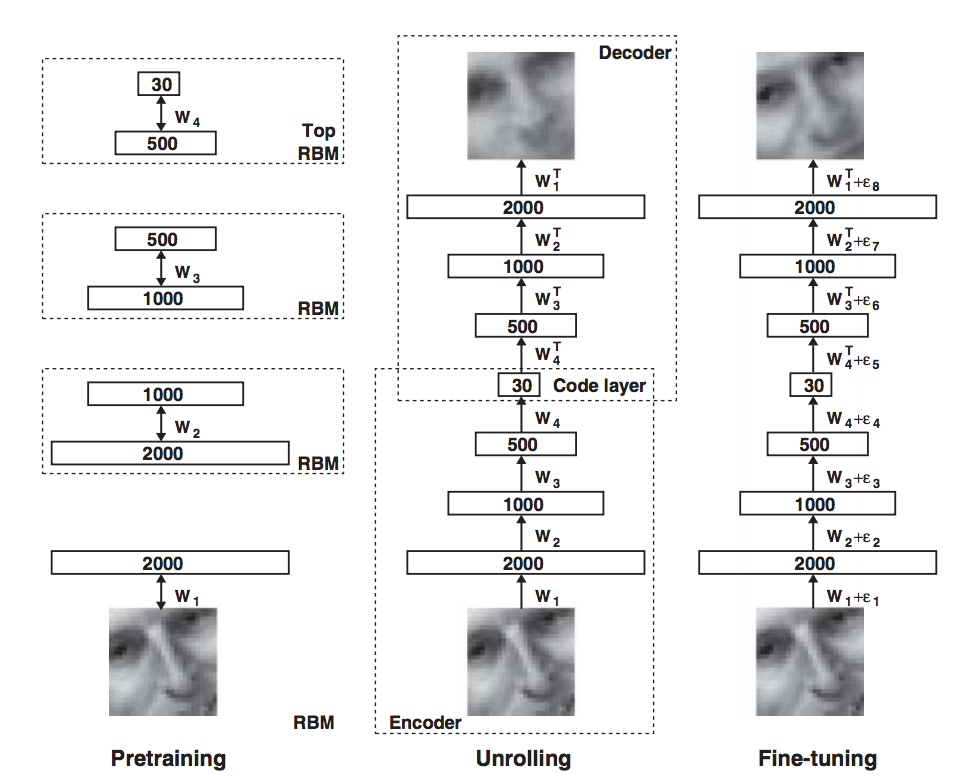
\includegraphics[scale=0.5]{images/DBN-RBM-process.png}
		\caption[The AutoEncoder Training Steps]{The AutoEncoder training steps \citep{Hinton2}}
		\label{figure-DBN-RBM}
	\end{figure}
	
	\subsubsection{Stacked Denoising AutoEncoders}\label{lr_SDAE}
	
	The second important piece of work was the development of a Denoising AutoEncoder (DAE), by \citet{Vincent}. 
	One of the problems identified in the DBN model described in Section \ref{DBN} (and those similar), is that if the encoder dimensions were too high, 
	it is likely that the encoder would learn a trivial encoding - essentially creating a ``copy the input'' model. The one way
	of tackling this issue is to constrain the representation with bottlenecks and sparse AutoEncoder layers, which can be seen in Figure \ref{figure-DBN-RBM}.
	\hfill \break 
	
	\citet{Vincent} explore a very different approach to the problem, which was to develop an implementation of 
	AutoEncoder which focused on partially corrupting the input, and so force the network to ‘denoise’ it. The theory 
	here is based on two ideas - the first, is that a higher dimensional representation should be robust to partial 
	corruption of the input data; and the second is that the denoising process will force model focus to shift to 
	extracting useful features from the input.
	\hfill \break 
	
	The algorithms and structures are largely the same as described for DBNs above, with the key difference 
	being that the model is trained to reconstruct the original input, but only using a corrupted version of the input 
	(where noise has been added to it), and so is forced to learn smarter feature mappings and extractions. 
	The DAE suggested then is a stochastic variant of the AutoEncoder, which has the benefit of being able to 
	implement higher dimensional representations without risking training of a trivial identity mapping. Notably, 
	in the Stacked Denoising AutoEncoder (SDAE) formation, only the initial input is corrupted (as opposed to the 
	input from layer to layer). It was shown that the SDAE model outperformed previous AE and DBN networks on 
	numerous benchmark datasets \citep{Vincent} . 
	
	\subsubsection{Pre-training}
	
	The methods described above follow a similar approach: greedy layer-wise unsupervised pre-training in order to 
	determine initial weights, followed by supervised fine tuning to arrive at the final model. It is shown numerous times, 
	that the pretraining process can result in significant performance gains \citep{Vincent}. However it is not immediately apparent, 
	given the nature of backpropagation algorithms and the like, why this is the case. \citet{Erhan} performed 
	extensive empirical simulations in order to suggest an explanation to the mechanism of pre-training.
	\hfill \break 
	
	While their results were not entirely conclusive, they did lend themselves to a reasonable hypothesis: 
	the unsupervised pre-training results in a form of regularization on the model - variance is minimized, and the 
	bias introduced acts as a prior to direct the model configuration towards a sample space that is effective for the unsupervised 
	learning generalization optimisations.
	
	\subsubsection{Time Series Applications}
	
	The AutoEncoder papers reviewed so far in this section derive their results primarily from classification problems, 
	and so do not necessarily account for the problems involved with time series as described in Section \ref{HDDR}. Due to 
	the inherent difficulties with predictions in the financial system, it can sometimes be unclear if the shortcoming in 
	results is due to this system complexity or if the methodologies used are unsuited for the purpose. In light of this 
	it is worth pointing out that Stacked AutoEncoder (SAE) implementations have been shown to be effective in many
	time series systems.  
	\hfill \break 
	
	\citet{Lv} implemented a deep learning SAE model using the methods described in Section \ref{lr_SDAE} in order to 
	predict traffic flow at various time intervals (15, 30, 45 and 60 minutes) - a problem not so structurally dissimilar 
	from what will be considered in this paper. They were able to show that the deep SAE was able to offer prediction 
	results which were both objectively good and also persistently outperformed the comparison models used 
	(backpropagation neural network, random walk forecast, support vector machine and a radial basis function 
	neural network).
	\hfill \break 
	
	In a review of unsupervised feature learning and deep learning methods on time series, \citet{Langkvist} noted that 
	the use of AutoEncoders, either as a technique in themselves, or as an auxiliary technique to models 
	such as convolutional neural networks, were able to offer performance increases in areas such as video analysis, 
	motion capture data and bacteria identification.
	
	\subsubsection{Financial Applications}
	
	There have of course also been successful applications of stacked AutoEncoders and deep learning models in 
	finance. \citet{Takeuchi} performed some earlier work showing the use of AutoEncoders when applied to a 
	momentum trading strategy. They implemented an RBM pre-trained DBN, as per Section \ref{DBN}, and assessed the 
	networks classification performance for ordinary shares on NYSE, AMEX and Nasdaq. This showed that using a 
	DBN network resulted in significant performance increases compared to the standard momentum strategy.
	\hfill \break 
	
	\citet{Zhao} used SDAEs and combined them with the bootstrap aggregation ensemble method (‘bagging’) in a 
	study of predicting the crude oil price. They compared the proposed model to a variety of benchmarks, including 
	standard SAE, bagged and standard feedforward networks and Support Vector Regression (SVR) models. The results indicated that the SAE models 
	were more accurate, with the bagged SAE model performing the best, though at a significant increase in 
	computational costs in comparison to standard SAE.
	\hfill \break 
	
	While much of the financial literature has focused on the use of RBM based models, AutoEncoders and SAEs have 
	recently been gaining popularity in performing feature reduction. \citet{Troiano} specifically investigate the use of 
	different feature reduction models for trend prediction in finance. In line with being primarily 
	interested in the effect of feature reduction techniques, rather than the classification performance itself, only a Support 
	Vector Machine (SVM) model was used to test results. Using various periods from historical S\&P500 data, they were able to show 
	that AE outperformed the RBM model significantly in numerous accuracy measures, and was able to do so at a 
	fraction of the training time.
	\hfill \break 
	
	\citet{Bao} note that the research has been lacking with regards to whether SAEs should be used for 
	financial prediction models or not. They suggest a novel model which combines Wavelet Transformation, SAEs 
	and a LSTM network. Using data from several financial exchanges (considering a 
	range of ‘developed’ and ‘undeveloped’ markets), they assess the model’s applicability to OHLC prediction. 
	Comparing the model to configurations without the SAE layers, and a RNN model as benchmark, they showed 
	that the inclusion of SAEs resulted in less volatility and greater accuracy, which in turn offered higher profitabilities 
	in a buy-and-hold trading strategy.
	\hfill \break 
	
	More novel AutoEncoder applications have also been attempted, with \citet{Hsu} suggesting the use of a 
	Recurrent AutoEncoder for multidimensional time series prediction. There is a clear pattern through the literature 
	that the use of AEs and SAEs both by themselves and when used as an assisting technique result in more accurate 
	prediction results and less computationally expensive training.
	
	\subsection{Online Learning Algorithms and Gradient Descent} \label{lr_OGD}
	\hfill
	
	Most classic machine learning algorithms operate under the assumption that, for all intents and purposes, the 
	full dataset has been collected and that the amount of training data for the model is both finite and immediately 
	available. However, as the growth of information grows in an exponential fashion, there are numerous areas where
	the expected training data for the model will continue to grow. In these cases it would be disadvantageous to go 
	through the full training and validation process again in order to incorporate the newly available data.
	\hfill\break
	
	Online algorithms are designed to offset these issues by adjusting the batch training technique to rather 
	repetitively draw on single samples from the data on which the model’s parameters can be adjusted. The benefit 
	is that they are able to quickly process a large number of observations and readjust the model, though the 
	downfall is that they are not always able to optimize the cost function to the same extent as offline batch 
	algorithms \citep{Albers}.
	\hfill\break
	
	\citet{Bottou} argue that as the size of the dataset grows significantly, online algorithm's advantages result in 
	them outperforming offline models, despite any initial drawbacks. Previous research had shown that online 
	algorithms typically perform as fast as batch algorithms during the `search' phase of parameter optimization, but 
	that `final' phase convergence tended to fluctuate around the optima due to the noise present in single sample 
	gradients \citep{LeCun, Bottou2}. \citet{Bottou} showed that it is actually more practical to consider the convergence towards
	the parameters of the optima, rather than the optima itself (as defined by the cost function) - the difference 
	between the learning speed and optimization speed, respectively. Online learning methods are thus well suited to financial market modelling using neural networks. They allow effective and efficient incremental updates as more recent (and relevant) data 
	becomes available. Further, the increased learning speed over optima convergence makes them a fitting choice when data is non-IID and 
	constantly changing.
%	Theoretical and empirical findings were 
%	presented to show that a stochastic online gradient descent algorithm was able to 
%	outperform the batch model for parameter estimation, and was able to asymptotically outperform in the number of 
%	samples processed in a time period. The stochastic aspect of the algorithm is related to random observations 
%	from batch sample groups being used as the gradient basis. Theoretically, this slows down the convergence, but 
%	speeds up the processing speed of each batch - a technique which has later been shown to be generally 
%	successful \citep{Shalev, Zhang}. 

	
	
	
	\subsection{Gradient Learning Improvements}\label{lr_grad_improv}
	
	\subsubsection{Gradient Adjustments and Regularization}
	
	One of the earlier improvements to convergence rates was the Momentum algorithm, as developed by \citet{Tseng}. 
	As noted, stochastic descent often introduces significant oscillation around an optima, which slows down 
	convergence. Momentum reduces this by decreasing movement in directions of high curvature, and  
	increasing movement towards directions consistent with previous gradients (this is achieved through combining 
	gradient movements in opposite directions).
	\hfill\break
	
	There have been several attempts to introduce effective regularization into the SGD process. \citet{Bartlett} 
	presented Adaptive Online Gradient Descent, which implements an adaptive step size through a $\lambda$ 
	penalty on the learning rate, which was shown to be nearly optimal in a strong sense. Langford et al. 
	demonstrated a variation named Truncated Gradient, which introduced an enforced weight sparsity parameter. 
	The weight sparsity is able to achieve equitable effects to $L_1$ regularization (similar to Lasso Regression). 
	They were able to show that implementation performed effective feature reduction, while having little effect on 
	performance \citep{Langford}. Other approaches, such as AdaGrad, aim to improve the robustness of gradient training by 
	adjusting the updates to parameters according to frequency - e.g. larger updates to infrequent parameters, and 
	smaller updates to frequent parameters \citep{Duchi, Zeiler}. 
	\hfill\break
	
	\subsubsection{Dropout}
	
	One of the instrumental improvements in further achievements, was to modify the backpropagation 
	algorithm using the ``dropout'' technique, as suggested by \citet{Hinton4}. When training of large networks is 
	attempted on small datasets, it often results in overfitting and poor results on out of sample data. Dropout helps 
	resolve this by randomly excluding a certain percentage (usually 0.5) of feature detectors on each training iteration. 
	The effect is to stop co-adaptations of feature detectors, and by rather training each neuron in a wide variety of 
	internal configurations, it forces them to take on more usefully generalizable characteristics (it was noted that this
	is not a dissimilar technique to ensemble methods, or bagging). The authors were able to show that the method
	results in significant improvements on benchmark data sets (e.g. MNIST, CIFAR-10), and that a simpler model 
	using dropout was able to achieve near comparable performance for the ImageNet dataset.
	\hfill \break 
	
	\citet{Goodfellow} used the dropout technique as the basis for their ``maxout'' activation function technique, which 
	leverages and improves on dropout\textsc{\char13}s fast optimisation and accuracy through averaging characteristics. The 
	maxout model was shown to achieve state of the art performance on benchmark datasets, as well as have a 
	strong theoretical grounding. Further work was done by \citet{Wang2}, which improved on the dropout 
	(and potentially maxout) techniques through fast sampling, resulting in an order of magnitude speed-up in
	training.
	\hfill \break 
	
	
	
	\subsubsection{Learning Rate Schedules}
	
	Several more recent approaches look towards learning rate adjustment schedules rather than strategies to alter the 
	weight update, as with momentum and the like. A constant learning rate often suffers from one of two problems - 
	if set too high, it can cause divergent behaviour in the loss function, though if set too low, it can result in slow 
	learning or an inability to escape saddle points effectively. Finding an optimal learning rate requires some degree
	of testing, though even then a singular value may fail to achieve the same degree of efficacy as a range of values 
	explored throughout the solution space. \newline
	
	Learning rate scheduling has been proposed as a solution to this problem. These methods implement a repetitive cycle 
	for the learning rate, such that it is set through a range of values between a minima and maxima, being adjusted slightly 
	with each new epoch. \citet{Smith} suggests using the Cyclical Learning Rate (CLR) to achieve this, and points out that part of the benefit 
	in learning rate schedules is the ability to jump out of sharp optima points which may not generalise well to unseen data. 
	It's shown that this implementation can have significant performance effects in reaching either the same optima in fewer epochs or a better 
	overall optima, including when used in conjunction with other learning optimizations noted in Section \ref{lr_grad_improv}. These results were 
	shown against standard datasets such as CIFAR-10, CIFAR-100 and ImageNet \citep{Smith}. \newline
	
	Similarly, \citet{Loshchilov}, expand on this and present Stochastic Gradient Descent with Warm Restarts. The approach is 
	implemented similarly, but rather follows an asymmetric cycle from a maximum to a minimum, and then starting once again at the maximum once the set number 
	of epochs has passed. They too note the increased performance on CIFAR-10 and CIFAR-100 datasets in reaching optima far quicker, as well as noting the efficacy of the 
	learning rate schedule even without implementing the restarts.
	
	
	
	\subsection{Backtesting and Model Validation} \label{lr_backtesting}
	\hfill
	
	Financial academic literature is currently facing a problem in terms of validation and verification of results. 
	Trading strategy profitability has typically been proven using historical simulations, or 
	``backtests''. However, 
	the recent advances in technology and algorithms available 
	to construct these strategies have resulted in researchers being able to test a number of variations that is factors 
	above what used to be possible. This has made it increasingly difficult to control for spurious results. 
	The problem is so extensive that some meta-research papers suggest that ‘most published research findings are false’ \citep{Ioannidis}.
	\hfill \break 
	
	The standard way of implementing backtests is to split the data into two portions: an In Sample (IS) portion which
	is used to train the model, and an Out of Sample (OOS) portion which is used to test the model and validate results. 
	If millions of different model configurations are tested, then it is only a matter of time before a false positive result occurs which shows high performance both IS and OOS (i.e. overfitting) \citep{BailyPBO, McLean}. 
	\hfill \break 
	
	The nature of financial data makes it difficult to resolve these issues effectively. There is a low signal-to-noise ratio in a dynamic and adaptive system, and 
	only one true data sequence. Traditional hypothesis testing frameworks (e.g. Neyman-Pearson) are not sufficient in this context, and more sophisticated techniques are necessary.
	\hfill \break 
	
	Overfitting is not a novel issue. This has been tackled in various literature areas, including machine learning. 
	However, in that context, the frameworks are often not suited to the buy/sell with random frequency structure of 
	investment strategies. They also do not account for overfitting outside of the output parameters, or take into 
	consideration the number of trials attempted.
	
	\hfill \break 	
	One of the common approaches to avoid backtest overfitting is the ‘hold-out’ strategy, where a certain portion of 
	the dataset is reserved for testing true OOS performance. Numerous problems have been pointed out with this 
	approach, including that the data is often used regardless, or that awareness of the movements in the data may, 
	consciously or otherwise, influence strategy and test design by the researchers \citep{Schorfheide}. For small samples, 
	a hold-out strategy may be too short to be conclusive \citep{Weiss}, and even for large samples it results in the 
	most recent data (which is arguably the most pertinent) not being used for model selection \citep{Hawkins, BailyPBO}.
	\hfill \break 
	
	There have been some suggestions to resolve the problem that is occurring in the literature as a result of this - some 
	work suggesting new frameworks, which this section will cover, and others which focus on the review process or 
	how data and replication procedures are made available \citep{Prado}. The points made with regard to the review and data processes are important, 
	but do not aid with more effective model training for the researcher up front and so are not covered here.
	
	\subsubsection{Sharpe Ratio Assessment Methodologies}\label{lr_backtest_sr}
	
	
	The Sharpe Ratio (SR), as introduced by \citet{Sharpe} in earlier literature, has become the favoured choice as a widely usable
	investment portfolio performance measure \citep{BaileyFrontier}. The measure, indicating the amount of return relative to risk that a portfolio offers, makes for 
	a sensible choice in that any portfolio which maximizes this can be shown to lie on Markowitz's efficient frontier. In line with its popularity, there has been 
	extensive research around its distributional properties. \citet{Lo} shows that the estimated SR of a portfolio's returns has been shown to follow a normal distribution, regardless
	of whether the underlying returns are themselves normally distributed or not. Further work by \citet{Christie} and \citet{Opdyke} derived a limiting distribution, assuming only stationary and ergodic returns.
		\hfill \break 
		
	The Sharpe Ratio, and indeed most standard performance measures, are based on the assumption that the returns used are the result of a single trial. In consideration of the issues laid out above, it then becomes a misrepresentative performance measure. \citet{BaileyFrontier} expanded on the work by \citet{Christie} and \citet{Opdyke} and developed the Probabilistic Sharpe Ratio (PSR) in order to estimate the likelihood that an observed best estimated $\widehat{SR}$ exceeds a provided benchmark $SR^{*}$, which might be expected from variance in the trials. 
	\hfill \break 
	
	It is worth emphasising the distinction in investment strategies between a Family Wise Error Rate (FWER), which is the  probability that one or more false positives occur, and a False Discovery Rate (FDR), which is the ratio of false positives to predicted positives. Where an FDR based approach may be applicable to a manufacturing process where there is an acceptable defect rate, investment strategy generations will tend to rely on the single best approach produced. Necessarily then, the FWER must be controlled for. Further work by \citet{BaileySharpe} developed the False Strategy Theorem (FST) with this in mind, allowing the assessment of whether a presented strategy is a false positive or not.
		\hfill \break 
	
	 This allowed the development of the Deflated Sharpe Ratio (DSR) which calculates the likelihood that the true SR is positive under consideration of numerous trials being tested \citep{BaileySharpe}. The DSR can be estimated using the PSR methodology as $\widehat{PSR}[SR^*]$ where the benchmark $SR^{*}$ (SR) is no longer user defined, but rather calculated based on the False Strategy Theorem. That said, the calculation of $SR^{*}$ requires both the variance of trial SR values the number of independent trials, which are usually unknown on accounts of being meta-research variables which cannot be estimated from the selected strategy. It is not typical for researchers to track and report on these variables, and even if they were to, the trials would not typically be independent, thus further complicating the practical realities around calculating $SR^{*}$. \citet{PradoDSR} provide critical work to this end with the Optimal Number Clusters (ONC) algorithm. They present a modified K-means methodology of clustering strategies and trial results, such that the dependent returns are categorised into subgroups with high intra-cluster correlations and low inter-cluster correlations. This clustering allows an estimation then of both the variance and number of trials, which in turn allows the DSR to be calculated. With this as a confidence level, one can accept or reject the notion that the observed $\widehat{SR}$ is positive.
		\hfill \break 
		
	The approach developed by \citet{PradoDSR} (of combining PSR, FST, DSR and ONC) relies on several principles which may differ from prior methods suggested (such as those by \citet{Harvey}). The first is that returns do not always follow a normal distribution, which is supported by empirical evidence, and so their method rather takes into account the skewness and kurtosis of observed returns. The second is that Extreme Value Theory is a more appropriate technique than something such as Sidak's correction, due to the incorporation of return variance when a non-normal distribution is present. The third is that they do not assume a  constant average correlation across trials, noting that there is often a hierarchical structure amongst returns where there may be highly correlated clusters of strategies. Failing to take this into account would then bias the expected number of independent trials and so the false positive probability. 

	\subsubsection{Generalised Assessment Methodologies}\label{lr_backtest_cscv}
	
	There has been work by several authors to try and lay out alternative techniques to try and avert backtest overfitting. 
	The Model Confidence Set (MCS), as developed by \citet{Hansen}, starts with a 
	collection of models or configurations, and removes models iteratively according to a defined loss function. 
	The confidence set is defined by the remaining models once a non-rejection takes place within the process, and 
	these models are considered to be statistically similar within a certain confidence range. MCS is thus able to facilitate 
	equitable model selection. However, \citet{Aparicio}, showed that while MCS is a potential strategy, in 
	practice is is ineffective due to the inordinate requirement of signal-to-noise necessary to identify true superior 
	models, as well as a lack of penalization over the number of trials attempted.
	\hfill \break
	
	\citet{BailyPBO} have developed a more robust approach to backtesting and how overfitting during strategy 
	selection might be avoided, called Combinatorially Symmetric Cross-Validation (CSCV). Their research defines backtest overfitting as having occurred when the strategy selection which maximizes IS performance systematically underperforms the median OOS performance in comparison to the remaining configurations. They use this definition to develop a framework which measures the probability of such an event occurring, where the sample space is the combined pairs of IS and OOS performance of the available configurations. The Probability of Backtest Overfitting (PBO) is then established as the likelihood of a configuration underperforming the median IS while outperforming IS. 
	\hfill \break 
	
	The CSCV methodology provides several important benefits over traditional testing 
	frameworks, including the usual K-fold cross validation used in machine learning. By recombining the slices of 
	available data, both the training and testing sets are of equal size, which is particularly advantageous when comparing 
	financial statistics such as the Sharpe Ratio, which are susceptible to sample size. Additionally, the symmetry 
	of the set combinations in CSCV ensure that performance degradation is only as a result of overfitting, and not 
	arbitrary differences in data sets. It is pointed out that while CSCV and PBO should be used to evaluate the quality 
	of a strategy, they should not be the function on which strategy selection relies, which in itself would result in overfitting. In this sense, the methodology helps assess overfitting, but not necessarily avoid it. Another of the noted limitations of the framework is 
	that a high PBO indicates overfitting within the group of N strategies, which is not necessarily indicative that none 
	of the strategies are skilful - it could be that all of them are. 
	\hfill \break 
	
	\subsubsection{Test Data Length}

	When using SR estimations, where it is possible that the true SR mean is 
	zero, we may still (with enough configurations attempted) find an SR measurement which optimises IS performance. 
	This is shown by \citet{BaileyBTL}, who propose the non-null probability of selecting an IS strategy with null expected 
	performance OOS. Notably, typical methods such as hold-out once again fail, as the number of configurations 
	attempted are not recorded. They add a further derivation, which is the Minimum Backtest Length (MinBTL), a statistic which highlights the relationships between: selecting a strategy with a higher IS SR than the expected OOS SR, 
	the number of strategies tested, and the number of years tested. The equation shows that  as the number 
	of strategies tested increases, the minimum back test length must also increase in order to contain the likelihood 
	of overfitting to IS SR. 
	\hfill \break 
	
	As shown extensively throughout ML literature, increased model complexity and number of parameters is one of 
	the primary causes of overfitting. In context of the MinBTL formula, model complexity affects the number of 
	configurations that are available and which may be tested, which in turn will increase likelihood of overfitting. 
	A lack of consideration, or reporting, of the number of trials makes the potential for overfitting difficult to assess. 
	\hfill \break 
	
	\citet{BaileyBTL} expanded on this view with assessing the impact of presenting overfit models as correct. 
	They were able to show that in lieu of any compensation effects (i.e. a series following a Gaussian random walk), 
	there is no reason for overfitting to result in negative performance. However, where compensation effects apply 
	(e.g. economic/investment cycles, bubble bursts, major corrections etc.), then the inclusion of memory in a strategy
	is likely to be detrimental to OOS performance if overfitting isn’t controlled for.
	\hfill \break 
	
	\newpage
	
	\section{Data Processing and Generation }\label{Data}
	\subsection{Data Processing}\label{data_processing}
	
	The datasets used go through several transformations throughout the training and prediction process:
	
	\begin{enumerate}
		\item The raw data is log differenced and aggregated to rolling windows,
		\item The transformed data is split into Training and Prediction subsets,
		\item The predicted outputs have the scaling and log differencing reversed in order to reconstruct the actual price points.
	\end{enumerate}
		
	\subsubsection{Log Difference Transformation and Aggregation}\label{ldata_og_difference}
	All datasets are transformed into log feature fluctuation values, and are then aggregated to include fluctuations over rolling window periods. The log feature fluctuation for measured prices $\tilde{p}$ at timepoint $t$ is calculated using \eqref{eq_logdiff}:
	\begin{equation}\label{eq_logdiff}
	\Delta\mathbf{p}_i = \mathrm{ln(\tilde{p}_i) - \mathrm{ln}(\tilde{p}_{i-1})} .
	\end{equation}
	This log feature fluctuation is processed for each asset's closing price and for each time point $i$ (from the previous time point). The log fluctuations have the benefit of taking compound effects into account in a systematic way and are symmetric in terms of gains and losses. Further, the log transformation provides an ergodic time series which is indicative what will happen to $\mathbf{\tilde{p}}$ over time, and has been shown to be the correct optimization choice \citep{Peters}.
	\newline\newline
	The datasets are then expanded with the rolling window summations both in the past, for input, and in the future, for predicted output. A typical example would be past data aggregation windows of 1, 5 and 20, and a future prediction point of 5. These are calculated as summations of the log differences, such that for $d$ days:
	
	\begin{equation}\label{eq_price_agg_past}
	 \mathbf{p^{-}_{(d,t)}} = \sum_{i = t-d}^{t} \Delta\mathbf{p}_i , 
	\end{equation}
	
	\begin{equation}\label{eq_price_agg_future}
	 \mathbf{p^{+}_{(t,d)}} = \sum_{i = t+1}^{t+d} \Delta\mathbf{p}_i .
	\end{equation}
	
	Only data points with a full set of features are used for training and prediction.
	
	\subsubsection{Data Scaling}\label{data_scaling}
	Once the log differenced data has been aggregated using equations \ref{eq_price_agg_past} and \ref{eq_price_agg_future}, the datasets are either standardized or normalized to allow for better learning. Typical implementations of these methods are detailed below:
	
	\paragraph{Standardization}
	\begin{equation}
	\mathbf{z_i}= \mathrm{\frac{(\mathbf{p}_i - \mathbf{\bar{p}}) }{\sigma_p}}
	\end{equation}
	
	\paragraph{Normalization}
	
	\begin{equation}\label{eq_ltd_normalization}
	\mathbf{n_i}= 
	\frac{\mathrm{\mathbf{p}_i - \min\limits_{\mathbf{p}}}}
	{\mathrm{\max\limits_{\mathbf{p}} -\min\limits_{\mathbf{p}}}}
	\end{equation}
	
	~\\
	The framework presented here only uses the suggested variations, dubbed ``Limited Standardization'' and ``Limited Normalization'', which are used when the data is split up into the Training and Prediction sets. In this case all the data needs to be scaled, but the variance or range should not be travelling from the Prediction set to the Training set through the use of aggregated measures such as $\bar{\mathbf{p}}$. Thus, if the data is split at point $t$ out of $n$ data points, the scaling would be implemented as follows:
	
	\paragraph{Limited Standardization}
	
	\begin{equation}
	\mathbf{q_{(i, t)}} =\mathrm{ \frac{(\mathbf{p}_i - \bar{\mathbf{p}}_{1:t}) }{\sigma_{p_{1:t}}} , \forall  i \in (1, n)}
	\end{equation}
	
	\paragraph{Limited Normalization}
	
	\begin{equation}\label{eq_ltd_normalize}
	\mathbf{v_{(i, t)}}  = 
	\mathrm{ \frac{\mathbf{p}_i - \min\limits_{\mathbf{p_1},\dots\mathbf{p_t}}} 
		{\max\limits_{\mathbf{p_1},\dots\mathbf{p_t}} - \min\limits_{\mathbf{p_1},\dots\mathbf{p_t}}} 
		, \forall  i \in (1, n)}
	\end{equation}
	
	
	This log-differenced, aggregated and scaled data is then used as the input for the neural network models.
	
	\subsubsection{Reverse Data Scaling}\label{data_reverse_scaling}
	
	The predicted data points are transformed back into actual prices for returns analysis. The first step is to reverse the scaling that is done in Section \ref{data_scaling} in order to retrieve the log difference fluctuations. The reverse scaling equations are for a dataset of $n$ observations, which has been split at point $t$.
	
	\paragraph{Reverse Standardization}
	
	\begin{equation}
	\mathbf{z^{*}_i} = \mathrm{{\mathbf{z}_i} \cdot \sigma_p + \mathbf{\bar{p}}}
	\end{equation}
	
	\paragraph{Reverse Normalization}
	
	\begin{equation}
	\mathbf{n^{*}_i} = \mathrm{\mathbf{n}_i \cdot \left(\max_{\mathbf{p}} - \min_{\mathbf{p}}\right) + \min_{\mathbf{p}}}
	\end{equation}
	
	\paragraph{Reverse Limited Standardization}
	
	\begin{equation}
	\mathbf{q^{*}_i} = \mathrm{{\mathbf{q}_i} \cdot \sigma_{p_{1:t}} + \bar{\mathbf{p}}_{1:t}},  \forall  i \in (1, \mathrm{n})
	\end{equation}
	
	\paragraph{Reverse Limited Normalization}
	
	\begin{equation}
	\mathbf{v^{*}_i} = \mathrm{\mathbf{v}_i \cdot \left(\max\limits_{\mathbf{p_1},\dots\mathbf{p_t}} - \min\limits_{\mathbf{p_1},\dots\mathbf{p_t}}\right) + \min\limits_{\mathbf{p_1},\dots\mathbf{p_t}}},  \forall  i \in (1, \mathrm{n})
	\end{equation}
	
	
	\subsubsection{Price Reconstruction}\label{data_price_recon}
	
	The predicted log fluctuations produced in Section \ref{data_reverse_scaling} are used to reconstruct the predicted prices. 
	
	\begin{equation}\label{eq_price_recon}
	\mathbf{p^*_i} = \mathrm{\tilde{\mathbf{p}}_{i-d} \cdot e^{\hat{p}_{i}}}
	\end{equation}
	where:
	\begin{itemize}
		\item [] $\mathrm{\tilde{p}}$ = original asset prices,
		\item [] $\mathrm{\hat{p}}$ = predicted log fluctuation,
		\item [] $\mathrm{i}$ = price timepoint, and 
		\item [] $\mathrm{d}$ = price fluctuation prediction horizon.
		
	\end{itemize}
	\texttt{}\newline
	These reconstructed prices are then used to assess model returns later in the Money Management Strategy (Section \ref{imp_mms}).
	
	\subsubsection{Decorrelation}
	
	The data processing does not incorporate any sort of decorrelation processes or data ``whitening'' transformations, thus keeping all correlation relationships between asset price fluctuations intact.
	
	\subsection{Synthetic Data Generation}\label{data_synthetic}
	
	Synthetic data generation is implemented using Geometric Brownian Motion (GBM) as described in Algorithm \ref{algo_brownianmotion}, which allows the stocks simulations to be implemented with a drift ($\mu$) and variance ($\sigma$) for each stock. The GBM simulation has the benefit of generating prices in a random walk, such that future movements are independent of past prices and so suitable for emulating an efficient financial market. The implications of using such data are discussed more fully in Section \ref{results_synth}. Each dataset was generated with a random seed and using a Mersenne Twister pseudorandom number generator. \newline
	
	\RestyleAlgo{algoruled}
	\begin{algorithm}[H]
		\KwIn{$\sigma$, $\mu$, $\tilde{p}_0$, $n$}
		
		$t = \frac{1}{n}$\;
		$\mathbf{\tilde{p^s}}$ = [$\tilde{p}_0$]\;
		
		\ForEach{i in 1:n}
		{
			z = random()  $\sim \mathcal{N}(0,1)$\;
			$\tilde{p}^s_i = \tilde{p}^s_{i-1} \cdot e^{(\mu - \frac {\sigma^2}{2})t + \sigma  \sqrt{t}  z)}$\;
			$\mathbf{\tilde{p^s}}$ = [$\mathbf{\tilde{p^s}}$, $\tilde{p}^s_i$]\;
		}
		\KwResult{$\mathbf{\tilde{p^s}}$}
		\label{algo_brownianmotion}
		\caption{Geometric Brownian Motion Simulation}
	\end{algorithm}
	
	\subsubsection{GBM Data Distributions}
	
	An important aspect of GBM generated data is that the price changes follow a Log-Normal distribution. If this data is then processed as per the steps above in Section \ref{data_processing}, then after taking the log differenced values using equation \eqref{eq_logdiff}, the values will follow a Normal distribution. Once scaled using standardization or normalization, these values will become centred and possibly be following a standard normal distribution. However, due to the effect of the limited scaling techniques used, only the Training dataset will be consistent in following this distribution, with the Prediction dataset having an increasing number of outliers as the timepoint moves further away from the Training set demarcations. These issues have notable impacts throughout the results, and are discussed more in Section \ref{Results}.
	
	\subsection{Price Considerations}\label{data_prices}
	
	The ``Actual10'' dataset, as described in Section \ref{dataset_actual10}, is a price relative dataset. It should be noted that this does not account for inflation, which arguably makes the effective training of SAE and predictive networks more difficult. However, not being able to fully account for inflation would be an issue in any forward looking predictive model, and so it is sensible to keep it this way in our current dataset. It is also not expected to have a material impact on short term predictions, though it does make comparisons across time periods (i.e. IS and OOS) more difficult. Additionally, the dataset is price relative starting at 1.0, and so only price changes from the start onwards are accounted for and impact P\&L, rather than the initial starting prices which might have then caused some imbalances. This does not have a large impact on the process, but does mean the P\&L figures in the results section are of unit measures, rather than any particular currency.
	
	\newpage
	\section{Models and Algorithms}\label{Implementation}
	\subsection{Process Overview}\label{ProcessOverview}\label{imp_overview}
	
	
	The implementation focuses on bringing together several ideas: data reduction, deep learning with pre-training/weight initialization, online learning and backtest overfitting validation for the purposes of stock price prediction. The process implementation is discussed fully in Section \ref{imp_fullproc}, but can be summarised as per the steps below.
	
	\begin{enumerate}
		\item The dataset is split into 2 subsets: the Training portion, and the Prediction portion.
		\item The Training set is used to train the SAE and predictive FFN using the SGD algorithm. These networks are constructed with pre-training or weight initialization techniques.
		\item Once the SGD training is complete for the predictive network, the same Training dataset is used to generate the IS predictions to be used for the CSCV process.
		\item The Prediction set of data is used to continue training the network in an online manner using OGD.
		\item The predictions made during steps 3 and 4 go through reverse scaling, and prices are reconstructed.
		\item These reconstructed price predictions are used by the MMS to calculate returns and P\&L.
		\item The returns and P\&L calculated by the MMS are used by the CSCV process, to estimate the PBO or DSR figures.
	\end{enumerate}
	~\\
	The rest of this section will detail the algorithms used to train the relevant FFN, RBM and SAE networks, as well as the trading strategy and CSCV \& PBO testing procedures.
	
	\subsection{Feedforward Neural Networks}\label{imp_ffn}
	~\\
	Constructing Feedforward Neural Networks (FFN) in the form of multilayer perceptrons is a well established network technique, providing effective non-linear representations for both shallow and deep structures \citep{Schmidhuber}. Specifically, a FFN is made up of several non-cyclical layers: the first and last are the input and output layers, respectively, and any inbetween are referred to as `hidden' layers. Each layer is made up of nodes which are fully connected to the nodes in the previous and following layers, but do not have connections to nodes within the layer - information only travels forward. Each 
	node has an activation function, which acts on the weighted input from the previous layers' nodes.
	
	\begin{figure}[H]
		\centering 
		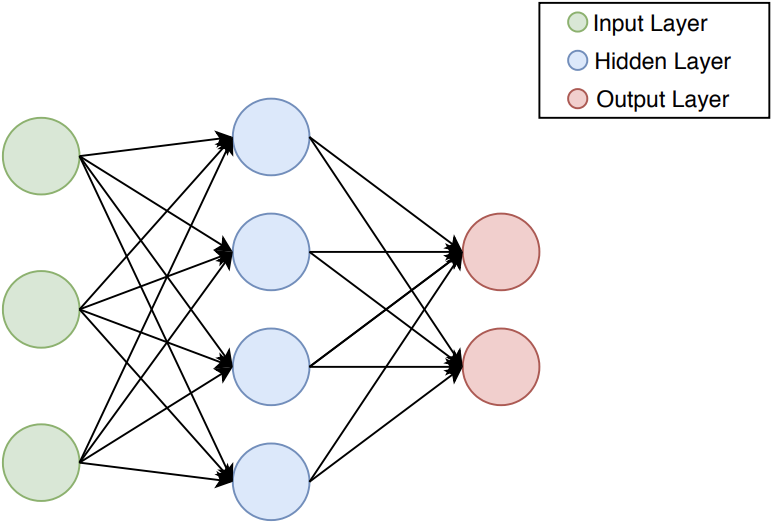
\includegraphics[scale=0.5]{images/implementation/neural_network_diagram.png}
		\caption[Feedforward Neural Network Diagram]{An example diagram of a Feedforward Neural Network with 1 hidden layer.}
		\label{figure-neural_network_diagram}
	\end{figure}		
	
	\subsubsection{Notation and Network Representation}\label{imp_ffn_functions}
	
	For the purposes of this section, the following notation will be used:
	
	\begin{itemize}
		\item[1] A network $N$ will be constructed with $L$ layers, each with $e$ nodes,
		\item[2] The weights from the $j^{th}$ node in the $\ell^{th}$ layer to the $k^{th}$ node in the $(\ell-1)^{th}$ layer are represented by $\mathbf{w}^\ell_{jk}$,
		\item[3] The bias for the $j^{th}$ node in layer $\ell$ is represented by $\mathbf{w}^\ell_{0j}$,
		\item[4] The output for the $j^{th}$ node in layer $\ell$ is 
		\begin{equation}\label{eq_activation_output}
		\mathbf{a}^\ell_j = \theta(\mathbf{z}_j) ,
		\end{equation} 
		for an activation function $\theta$ (with inverse $\mathrm{\theta^{\prime}}$) and weighted input $\mathbf{z}$, and
		\item[5] The weighted input for the $j^{th}$ neuron in layer $\ell$ is 
		\begin{equation}\label{eq_weighted_input}
		\mathbf{z^\ell_j}=\sum_{i=1}^{e^{\ell-1}}{\mathbf{a}^{\ell-1}_i\mathbf{w}_{ij}} + \mathbf{w}_{0j} .
		\end{equation}
	\end{itemize}
	~\\
	These definitions allow an input into the network to be propagated through it, having the original values processed through the weights and activations functions, and have an output in the form of the network's last layer.
	
	\subsubsection{Activation Functions}\label{imp_activation_functions}
	~\\
	As noted in Section \ref{lr_activationfunctions}, there are 3 primary characteristics of concern for activation functions: non-linearity, continuous differentiability and monotonicity. While many different functions have been suggested and used, several of the more popular were implemented here.
	
	\paragraph{Sigmoid}
	
	The sigmoid, or logistic, function is one of the most popular and widely used activation functions historically, and is defined as:
	\begin{equation}\label{func_sigmoid}
	\theta(x) = \frac{1}{1 + e^{-x}}, 
	\end{equation}
	
	\begin{equation}\label{func_sigmoidprime}
	\theta^\prime(x) = \theta(x)(1-\theta(x)).
	\end{equation}
	
	The Sigmoid function is in the range [0,1], making it a suitable choice for problems requiring a probabilistic output. The slope of the function curve is both a boon and a drawback: it allows for fast learning initially, but results in learning slowdown later (often causing what is referred to as node ``saturation''). The exponent calculation is also computationally expensive, relatively speaking.
	
	\paragraph{ReLU}
	
	The Rectified Linear Unit (ReLU) is a newer activation function which has been shown to be effective in deep learning networks. It is defined as:
	
	\begin{equation}\label{func_relu}
	\theta(x) = \max(0, x), 
	\end{equation}
	
	\begin{equation}\end{equation}\label{func_relu_prime}
	\[
	\theta^\prime(x)= 
	\begin{cases}
	1,& \text{if } x\geq 0\\
	0,              & \text{otherwise.}
	\end{cases}
	\]
	
	The function has the benefits of quick learning which doesn't saturate, as well as being computationally cheap. The downside is that the non-gradient for the negative range of the function can result in `dead' nodes, which stop updating with the learning process.
	
	\paragraph{Leaky ReLU}
	
	The Leaky ReLU resolves the dying ReLU problem by adding a small gradient to the negative range of the function. This results in a slow learning being applied to `dead' ReLU's, which may in turn result in them being used again if necessary. The choice of 0.01 as the negative range gradient in equations \eqref{func_leaky_relu} and \eqref{func_leaky_relu_prime} has been shown to be generally effective \citep{Maas}, though further work might investigate different parameter values for this. The Leaky ReLU activation function is defined as:
	

	\[
	\theta(x)= 
	\begin{cases}
	x,& \text{if } x\geq 0\\
	0.01x,              & \text{otherwise, }
	\end{cases}
	\]
	\begin{equation}\label{func_leaky_relu}
	\end{equation}
	
	\[
	\theta^\prime(x)= 
	\begin{cases}
	1,& \text{if } x\geq 0\\
	0.01,              & \text{otherwise.}
	\end{cases}
	\]
		\begin{equation}\label{func_leaky_relu_prime}
	\end{equation}
	
	\paragraph{Linear Activation}
	
	Linear activations don't transform the input, and have a constant gradient, which can be useful for key layers where no loss in error signal is desired, such as the output or encoding layers. The linear activation function is defined as:
	
	\begin{equation}\label{func_linear}
	\theta(x) = x, 
	\end{equation}
	
	\begin{equation}\label{func_linear_prime}
	\theta^\prime(x) = 1.
	\end{equation}
	
	\subsubsection{Backpropagation}\label{imp_backprop}
	
	The backpropagation algorithm, as discussed in Section \ref{lr_trainingbackprop}, has allowed for effective training of FNNs for given data. The algorithm relies on incremental improvements of the model, as defined by decreasing the cost function. A common choice for cost ($C$) is Mean Squared Errors (MSE):
	
	\begin{equation}\label{func_MSE}
	{C} = \frac{1}{2} \rVert \mathbf{y} - \mathbf{a}^L \rVert^2 .
	\end{equation}
	~\\
	
	The conceptual steps for the backpropagation (fully detailed in Algorithm \ref{algo_backprop}) are: \newline
	\begin{enumerate}
		\item \textbf{Forward Pass}: The samples are propagated through the network, in order to generate the output $\mathbf{a}^L$. \newline 
		
		Vectorization is typically used to calculate the results for multiple samples at once, though conceptually each sample is used as input for the first layer, and subsequent layers use the weighted output from the previous layer passed through the activation function as input.\newline 
		
		Equation \ref{eq_weighted_input} is used to calculate the weighted output and the equations defined in Section \ref{imp_activation_functions} are used for the activation functions.
		\newline
		
		\item \textbf{Calculate Cost}: The cost between the training output $\mathbf{y}$ and the model output $\mathbf{a}^L$ is calculated. \newline
		
		Using a cost function such as MSE (equation \eqref{func_MSE}), the rate of change for the error in the output layer by the rate of change in the output layer's activation functions is calculated. This rate of change for the error for the $j^{th}$ node, $\delta_j$, is expressed as:	
		
		\begin{equation}\label{eq_lambda1}
		\mathbf{\delta}_{j}^{L}=\frac{\partial \mathbf{C}}{\partial \mathbf{a}_{j}^{L}} \theta^{\prime}\left(\mathbf{z}_{j}^{L}\right) .
		\end{equation}
		
		The vectorized version of this is often used, and expressed in equation \eqref{eq_lambda2}. $\nabla_a C$ is a vector of components which are the partial derivatives, such that they represent the rate of change of cost $C$ relative to the activation functions' outputs.
		\begin{equation}\label{eq_lambda2}
		\mathbf{\delta}^{L}=\nabla_a \mathbf{C} \otimes \theta^{\prime}(\mathbf{z}^L), 
		\end{equation}
		where $\otimes$ is the Hadamard (or element-wise) matrix product.\newline
		
		If using quadratic cost, as per equation \eqref{func_MSE}, then the term $\frac{\partial C}{\partial a_{j}^{L}}$ can be reduced to $(a^L - y)$. The equation for the output layer error rate of change is then:
		\begin{equation}\label{eq_lambda3}
		\mathbf{\delta}^L = (\mathbf{a}^L - \mathbf{y}) \otimes \theta^{\prime}(\mathbf{z}^L) .
		\end{equation}
		\newline		
		\item \textbf{Backwards Pass}: 
		\begin{enumerate}
			\item \textbf{Calculate Errors For Previous Layers:} The activation values are propagated back through the network to calculate the delta values at each layer. \newline
			
			This uses the same rationale as equation \eqref{eq_lambda1}, but rather uses $(w^{\ell+1})^T$ by the next layers error in order to get an indication of the error rate and how it moves backwards through the network:
			\begin{equation}\label{eq_lambda4}
			\mathbf{\delta}^\ell = ((\mathbf{w}^{\ell+1})^T\mathbf{\delta}^{\ell+1})  \otimes \theta^{\prime}(\mathbf{z}^\ell) .
			\end{equation}
			
			\item \textbf{Adjust Network Weights:} Network weights are adjusted in proportion to the error observed and chosen learning rate.\newline
			
			Each weights output error and input activation are multiplied to find the weight’s gradient, which is then reduced by a factor of the ‘learning rate’ $\eta$. This adjustment value is subtracted from the current network weights:
			\begin{equation}\label{eq_bp_weightupdate}
			\mathbf{w}^\ell \rightarrow \mathbf{w}^\ell - {\eta}\mathbf{\delta}^{\ell} (\mathbf{a}^{\ell - 1})^T ,
			\end{equation}
			where $\eta$, the learning rate, is a configured parameter.
		\end{enumerate}
		
	\end{enumerate}
	
	Choices regarding the learning rates are discussed in Section \ref{imp_learning_rate_schedule} and the full algorithm is presented below in Algorithm \ref{algo_backprop}.\newline
	
	\RestyleAlgo{algoruled}
	\begin{algorithm}[H]
		\KwIn{Neural Network $N$, with randomly initialized weights $\mathbf{w}$, $L$ layers, activation functions $\theta$ and learning rate $\eta$}
		\KwData{Testing set with inputs $\mathbf{x}$, and outputs $\mathbf{y}$}
		
		\texttt{\\}
		
		\Repeat{no new samples can be drawn from $x$}{
			Select a sample $x_s$ from $x$\;
			
			\tcp{Perform the Forward Pass,  to calculate the network output, $y_s$, for input sample $x_s$}
			$a_0$ =  $x_s$;
			\texttt{\\}
			\ForEach{$\ell$ in 1:L}
			{
				\ForEach{j in 1:$e^\ell$}
				{
					$\mathbf{z}^{\ell}_j=\sum_{i=1}^{e^{\ell-1}}{\mathbf{a}^{{\ell-1}}_i\mathbf{w}_{ij}} + \mathbf{w}_{0j}$;
					\newline
					$\mathbf{a}^{\ell}_j$ = $\theta(\mathbf{z}^{\ell}_j)$;
				}
			} 
			\tcp{Calculate the error term (aka cost), as}
			$\mathbf{\delta}^L = (\mathbf{a}^L - \mathbf{y}) \otimes \theta^\prime(\mathbf{z}^L)$;
			
			\texttt{\\}
			\tcp{Perform the Backward Pass, to propagate the errors back and update the network accordingly}
			\ForEach{$\ell$ in (L-1):1}
			{
				\tcp{Calculate the delta values}
				$\mathbf{\delta}^\ell = ((\mathbf{w}^{\ell+1})^T\mathbf{\delta}^{\ell+1})  \otimes \theta^\prime(\mathbf{z}^\ell)$;
				
				\tcp{Update the weights}
				$\mathbf{w}^\ell \rightarrow \mathbf{w}^\ell - {\eta}\mathbf{\delta}^{\ell} (\mathbf{a}^{\ell - 1})^T$;
			}
		}
		
		\KwResult{Updated Network $N$}
		\label{algo_backprop}
		\caption{Backpropagation}
	\end{algorithm}
	
	
	
	
	\subsubsection{Gradient Descent Algorithms}\label{imp_sgd}
	
	The backpropagation algorithm is defined at a single sample level, and the learning from a dataset is usually repeated for a number of ``epochs''. As noted though, implementation is often implemented using a vectorized version of the algorithm which either samples the entire dataset at once (batch), or a subset of samples (mini-batch). The latter is the Stochastic Gradient Descent (SGD), as discussed in Section \ref{lr_OGD}, which has been shown to increase the speed and stability at which the backpropagation algorithm can converge to a minima in terms of cost. The algorithm runs backpropagation over the entire dataset for the number of epochs, and updates the network incrementally through the epoch. The stopping condition for the algorithm is usually defined as either a particular number of epochs being reached, or cost no longer decreasing for some number of epochs (i.e. a minima has been reached).\newline
	
	The changes to the initial backprop algorithm, detailed in Algorithm \ref{algo_backprop}, are relatively minor:
	\begin{itemize}
		\item [1] Selection is now performed such that at each epoch $m$, $s$ new samples are from $x$, forming the subset $x_s$.
		\item [2] The weight update is now performed such that it represents an aggregate update according the $m$ samples that were selected:
		\begin{equation}\label{eq_backprop_weightupdate_sgd}
		\mathbf{w}^\ell \rightarrow \mathbf{w}^\ell - \frac{\eta}{m} \sum_{x} \mathbf{\delta}^{x, \ell} (\mathbf{a}^{x, \ell - 1})^T , 
		\end{equation}
		where
		\begin{enumerate}
			\item $w^\ell$ is the $\ell^{th}$ layer's weights,
			\item $\eta$ is the configured learning rate parameter, 
			\item $m$ is the size of the mini-batch,
			\item $\delta$ is the rate of change in the error (calculated using equation \eqref{eq_lambda4}), and
			\item $a$ is the output of the activation function for the weighted input (calculated using equation \eqref{eq_activation_output}).
		\end{enumerate}
	\end{itemize}
	
	\subparagraph{Online Gradient Descent}
	Where SGD is appropriate and effective for scenarios where the entire dataset is available, Online Gradient Descent (OGD) is applicable for when the model is learning in an online fashion. In this case, the backpropagation is run as defined above in Algorithm \ref{algo_backprop} but with no repetition (i.e. only 1 epoch).
	
	\subsubsection{Regularization}\label{imp_regularization}
	
	Regularization is a commonly used technique in machine learning used to reduce a model's capacity to overfit to the data, and in so doing reduces the variance in the model results. One of the typical methods, ``$L2$'' (or ``weight decay''), is implemented by adding an extra term to the cost function which is itself a function of the weights in the model. This extra term forces the learning process to favour smaller weights, and only allows large weights to occur if they are able to offer an appropriate increase in performance. The modified cost function is calculated as:
	
	\begin{equation}\label{func_l2reg}
	\mathbf{C}=\frac{1}{2 n} \sum_{x}\left\|\mathbf{y}-\mathbf{a}^{L}\right\|^{2}+\frac{\mathrm{\lambda}}{2 n} \sum_{w} \mathbf{w}^{2},
	\end{equation}
	where
	\begin{enumerate}
		\item $n$ is the dataset sample size,
		\item $y$ is the input data,
		\item $a$ is the output of the activation function in the $L^{th}$ layer (calculated using equation \eqref{eq_activation_output}),
		\item $\lambda$ is the configured regularization rate, and
		\item $w$ is a layer's weights.
	\end{enumerate}
	
	The additional term is scaled by the configurable regularization parameter, $\lambda$, which if small approximates the original cost function or if large will increase the degree of regularization used. \newline
	
	In order to implement this in backpropagation, the weight update rule is changed to the following (while biases remain the same):
	
	\begin{equation}\label{func_l2_weight_update}
	\mathbf{w} \rightarrow \mathbf{w}-\eta \frac{\partial \mathbf{C}_{0}}{\partial \mathbf{w}}-\frac{\eta \mathrm{\lambda}}{n} \mathbf{w} .
	\end{equation}
	
	For SGD, this can be simplified to the following: 
	
	\begin{equation}\label{func_sgd_l2}
	\mathbf{w} \rightarrow\left(1-\frac{\eta \mathrm{\lambda}}{n}\right) \mathbf{w}-\frac{\eta}{m} \sum_{x} \frac{\partial \mathbf{C}_{x}}{\partial \mathbf{w}} .
	\end{equation}
	
	
	\subsubsection{Learning Rate Schedule}\label{imp_learning_rate_schedule}
	
	Learning rates schedules are implemented to allow for a more dynamic exploration of the possible solution space, and allow fine tuning around an optima. With a constant learning rate implementation, one has to choose between a larger learning rate which allows faster progress but less optimisation, or a smaller learning rate which learns slower but is more effective at optimising (by avoiding the learning algorithm from bouncing around a minima valley). Learning rate schedules aim to get the best of both scenarios by cycling through a minimum and maximum range across epochs.\newline
	
	The learning rate schedule is specified to cycle through from the minimum value to the maximum value every $T$ epochs, from $\eta_{\min}$ to $\eta_{\max}$. Thus for the current epoch $i$, the learning rate is calculated as:
	
	\begin{equation}\label{func_learning_rate_sched}
	\eta_{i}={\min\limits_{\eta} }+\frac{1}{2}\left({\max\limits_{\eta} }- {\min\limits_{\eta}}\right)\left(1+\cos \left(\frac{i}{T} \pi\right)\right) .
	\end{equation}
	
	This is the Cyclical Learning Rates approach, though using sinusoidal form rather than linear \citep{Smith}. For a minimum learning rate of 0.1, a maximum of 1.0 and an epoch cycle of 100, it will produce learning rates as displayed in Figure \ref{figure-SGDRLearningRates} below.
	
	\begin{figure}[H]
		\centering
		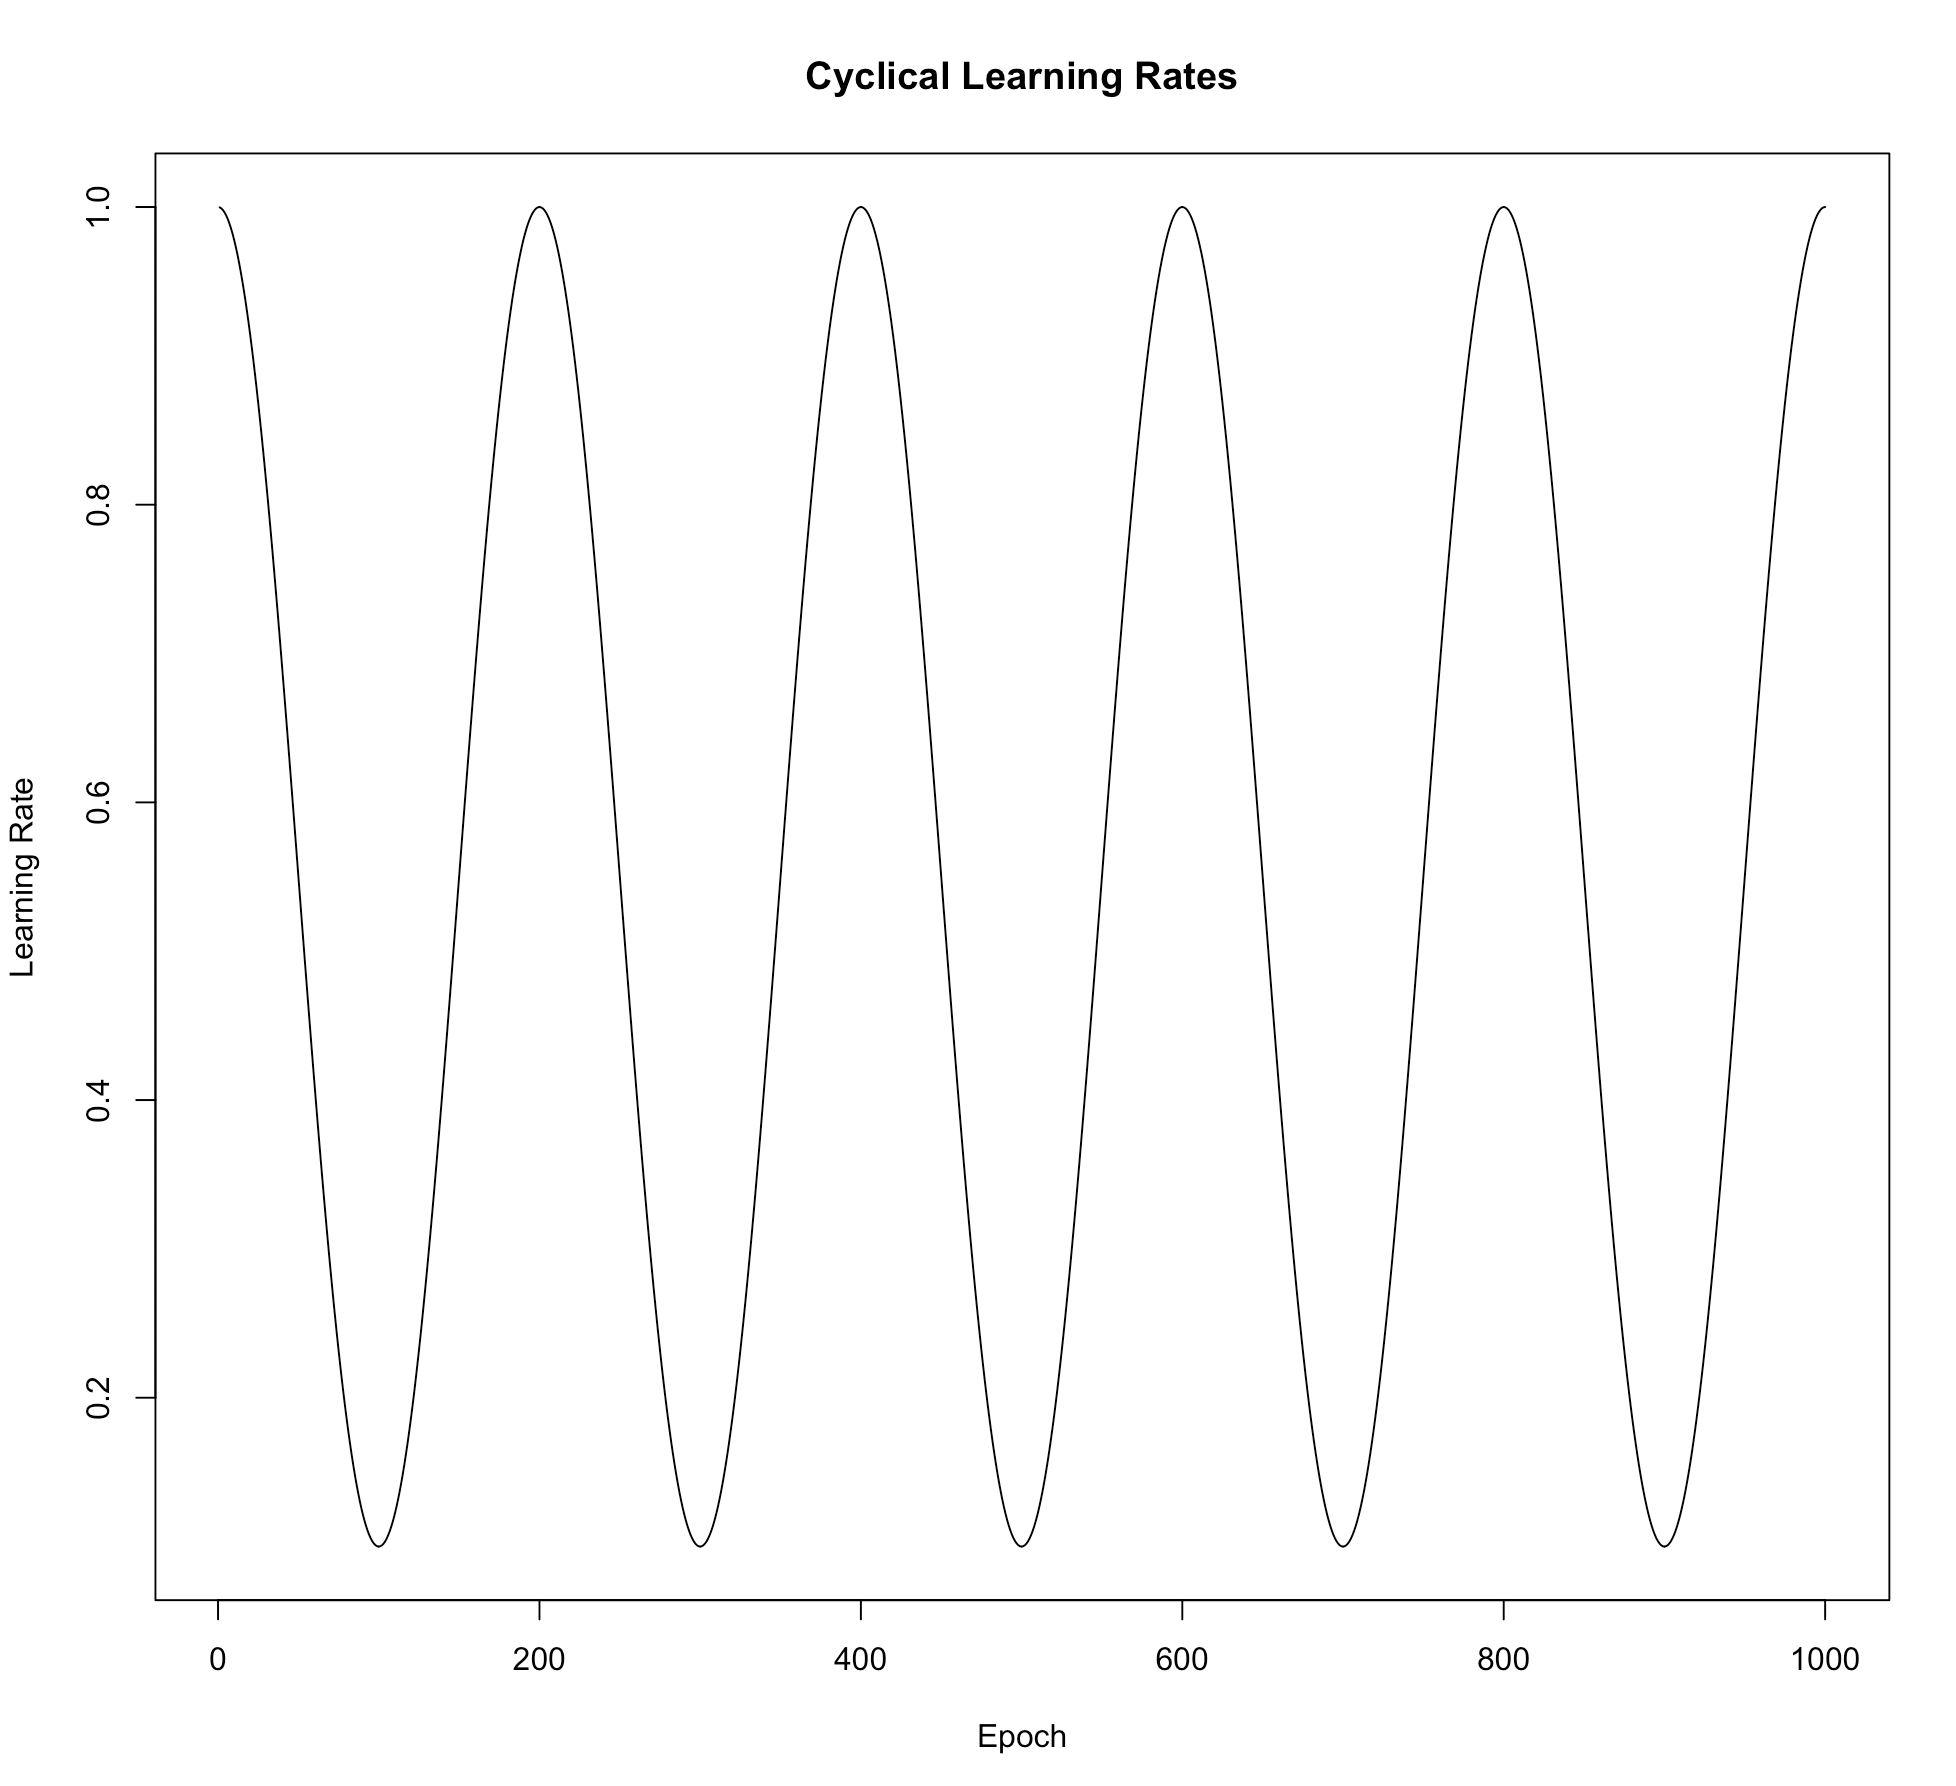
\includegraphics[scale=0.2]{images/implementation/CyclicalLearningRates.png}
		\caption[Cyclical Learning Rate Diagram]{Learning rates calculated over 1000 epochs with ${\min\limits_{\eta}} = 0.1$ to ${\max\limits_{\eta}} = 1.0$ and $i=100$.}
		\label{figure-SGDRLearningRates}
	\end{figure}
	
	\subsubsection{Dropout}\label{imp_dropout}
	
	Input layer dropout has been implemented in order to perform regularization on the data features. The methodology used will set a percentage of the features for each sample to 0 during the SGD training process. While the percentage stays the same throughout the testing process, the features selected for each sample are reselected every time it is used (i.e. for subsequent epochs). Conceptually, the dropout as applied to the input layer may result in the network learning relations between assets and possible patterns that would improve predictive efficacy.
	
	\subsection{Restricted Boltzmann Machines}\label{imp_rbm}
	
	Restricted Boltzmann machines (RBM) are generative networks which can be trained to learn probability distributions over a dataset. They are structurally different from a FFN in that they have a recurrent weight structure and stochastic unit determination. Specifically, a typical RBM has one visible layer (input/output), and one hidden layer, and the values in the hidden layer will take on a binary value with a probabilistic likelihood.  \newline
	
	Thus, the input and output have the same structure, and the processing from the hidden layer creates the generative process learned by the RBM. The hidden units correspond to feature detection of the visible unit data structures, and the learning process of the network results in effective parameter estimation. \newline
	
	\begin{figure}[H]
		\centering 
		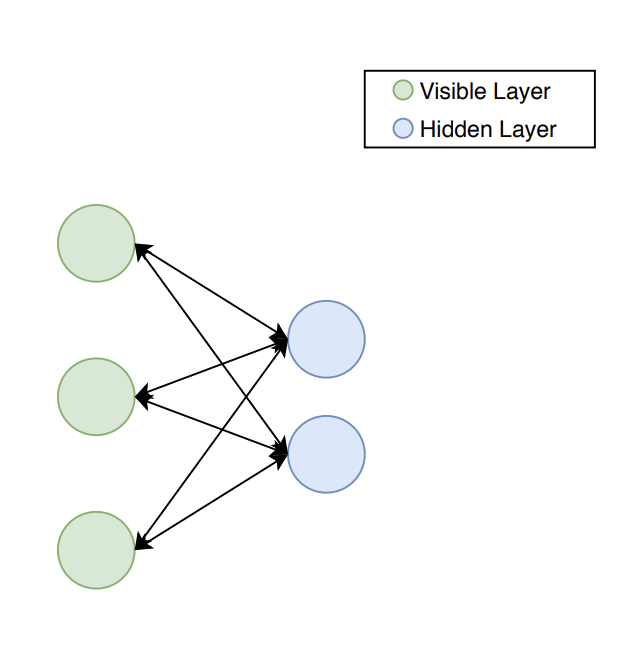
\includegraphics[scale=0.5]{images/implementation/rbm_network_diagram.png}
		\caption[Restricted Boltzmann Machines Diagram]{An example diagram of a restricted Boltzmann machine network.}
		\label{figure-rbm_network_diagram}
	\end{figure}		
	
	RBM input processing goes through the following steps:
	
	\begin{enumerate}
		\item An input sample, $\mathbf{y}$, is processed from the visible layer to the hidden layer using typical feedforward functions.
		\item Each node in the hidden layer takes on a value of 1 with a probability of its activation function output, or else is equal to 0.
		\item The visible layer nodes are reconstructed to provide $\mathbf{\hat{y}}$, using the hidden layer values as the input.
	\end{enumerate}
	
	\subsubsection{RBM Stochastic Descent}
	
	\citet{Hinton5} shows that the joint configuration $(v,h)$ of the visible and hidden units has an energy given by :
	
	\begin{equation}\label{func_rbmenergy}
	E(\mathbf{v},\mathbf{h}) = - \sum_{i \in visible} \mathbf{a}_i\mathbf{v}_i - \sum_{j \in hidden} \mathbf{b}_j\mathbf{h}_j - \sum_{i,j}\mathbf{v}_i\mathbf{h}_j\mathbf{w}_{ij}
	\end{equation}
	
	, where
	\begin{enumerate}
		\item $\mathbf{v}$ and $\mathbf{h}$ are the binary state vectors of the visible and hidden units respectively, 
		\item $\mathbf{a}$ and $\mathbf{b}$ are the bias value vectors for the visible and hidden units respectively, and
		\item $\mathbf{w}$ is the weights vector for the 2 visible and hidden layers.
	\end{enumerate}
	~\\
	It can be shown, that network weights can be adjusted to change the probabilities assigned to a particular training sample . The derivations of equation \eqref{func_rbmenergy} show that performing a stochastic descent for the log probability of the data can be implemented through the following weight adjustment:
	
	\begin{equation}
	\Delta \mathbf{w}_{ij} = \eta (\langle \mathbf{v}_i\mathbf{h}_j\rangle_{data} - \langle \mathbf{v}_i\mathbf{h}_j\rangle_{model}) .
	\end{equation}
	
	The angular brackets here indicate expectations under the distribution specified by the following subscript. Due to the probabilistic nature of RBMs, the [0,1] ranged Sigmoid activation function is typically used. Thus, for hidden nodes and a data sample $v$, it is easy to get unbiased sampling of $\langle v_ih_j \rangle_{data}$
	
	\begin{equation}
	\mathrm{P}(\mathbf{h}_j=1) = \sigma(\mathbf{w}_{0j} +  \sum_{i=1}\mathbf{v}_i\mathbf{w}_{ij})
	\end{equation}
	
	Similarly, the visible states (or reconstruction), can then be calculated as 
	
	\begin{equation}
	\mathrm{P}(\mathbf{v}_i=1) = \sigma(\mathbf{w}_{0i} + \sum_{j=1}\mathbf{h}_j\mathbf{w}_{ij})
	\end{equation}
	
	
	Getting an unbiased sample of $\langle v_i h_j \rangle$ proves more problematic, and so the model reconstructions via Gibbs sampling are used instead (this is expanded on below), resulting in the weight updates of
	
	\begin{equation}
	\Delta \mathbf{w}_{ij} = \eta (\langle \mathbf{v}_i\mathbf{h}_j\rangle_{data} - \langle \mathbf{v}_i\mathbf{h}_j\rangle_{reconstruction})
	\end{equation}
	
	While it is important for the hidden units to take on a binary value (and so avoid communicating real values rather than learning structure), the visible units may be chosen to take on the probability values, rather than the stochastic samples, particularly if real valued output is necessary. 
	
	\subsubsection{Contrastive Divergence}\label{imp_CD}
	
	The process of sampling and resampling may be run for many iterations between the two layers before finishing on an output - this potentially long running and stochastic process results in the generative aspect of the network, and constitutes a Gibbs sampling chain. Multiple sampling steps in this chain is known as Contrastive Divergence, or CD-n, where $n$ represents the number of steps, and which allows for effective parameter estimation. CD-1 is detailed in Algorithm \ref{algo_cd1}.\newline
	
	
	\begin{algorithm}[H]
		\KwIn{RBM Network $N$, with visible nodes $\mathbf{v}$ and hidden nodes $\mathbf{h}$ and weight distribution $\mathbf{w}$ (representing $\langle vh\rangle$)}
		\KwData{Training sample dataset $D$}
		
		\texttt{}\newline
		
		\ForEach{$\mathbf{V^D}$ in $D$}
		{
			~\\
			\tcp{Sample $\mathrm{H^D}$ from $\mathrm{P(H^D|V^D)}$}
			\ForEach{$n$ in (1:j)}
			{
				$\mathrm{P}(\mathbf{H^D}_n=1) = \sigma(\mathbf{w}_{0j} +  \sum_{i=1}\mathbf{V^D}_i\mathbf{w}_{in})$
			}
			~\\
			\tcp{Sample $\mathrm{V}$ from $\mathrm{P(V|H^D)}$}
			\ForEach{$n$ in (1:i)}
			{
				$\mathrm{P}(\mathbf{V}_n=1) = \sigma(\mathbf{w}_{0i} + \sum_{j=1}\mathbf{H^D}_j\mathbf{w}_{ij})$
			}
			~\\

			\tcp{Sample $\mathrm{H}$ from $\mathrm{P(H|V)}$}
			\ForEach{$n$ in (1:j)}
			{
				$\mathrm{P}(\mathbf{H}_n=1) = \sigma(\mathbf{w}_{0j} +  \sum_{i=1}\mathbf{V}_i\mathbf{w}_{in})$
			}
			~\\

			\tcp{Calculate Change in Weights Using Reconstructed Distribution}
			\tcp{$\Delta \mathbf{w}_{ij} = \eta (\langle \mathbf{v}_i\mathbf{h}_j\rangle_{data} - \langle \mathbf{v}_i\mathbf{h}_j\rangle_{reconstruction})$}
			$\Delta \mathbf{w} = \eta ([{\mathbf{V}^D}{\mathbf{H}^{DT}}] - [\mathbf{V}\mathbf{H}^T])$

			\texttt{}\newline
			
			\tcp{Update the weights}
			$\mathbf{w} \rightarrow \mathbf{w} - \Delta \mathbf{w}$
		}

		
		%For a random training sample $V'$, sample $H'$ from $P(V|H)$;
		%Sample $V$ from $P(V|H')$;\newline
		%Sample H from $P(H|V)$;\newline
		%Return $(V,H) \sim R $, where R is the reconstructed distribution for $\langle vh \rangle$;\newline		
		%\tcp{Using the reconstructed distribution $R(V,H)$, the weight update for CD-1 is, as above, then}
		%\Delta CD(W) = \eta( E_{P(H|V)D(V)}[VH^T] - E_{R(V,H)}[VH^T])		
		\KwResult{Network $N$ with weights $\mathbf{w}$ updated for dataset $D$}
		
		\label{algo_cd1}
		\caption{CD-1}
	\end{algorithm}
	~\\
	There's no upper bound on the iterations used for CD, and running for many can prove more effective for certain purposes. In this case however, where RBMs are used for the purposes of weight initialization, CD-1 is usually deemed sufficient.
	
	\subsubsection{CD-1 and SGD}
	
	In the same way that the backpropagation learning algorithm in Section \ref{imp_backprop} can be implemented in a mini-batch SGD process for FFNs, so can the CD learning algorithm for RBMs. The framework is kept the same, with the implementation of epochs and weight updates based on stochastically chosen minibatches, but the calculation used to update the weights is CD-1 instead.
	
	
	\subsection{Stacked AutoEncoders}\label{imp_SAE}
	
	As noted in Section \ref{lr_SAE}, the use of Stacked AutoEncoders (SAE) have resulted in significant improvements in deep learning networks, and allowed effective reduction of high dimensional data. A single layer AutoEncoder is a specialized type of FNN with 3 layers: one input, one hidden, and one output. The network is trained (using backpropagation as per Section \ref{imp_backprop}) to reconstruct the input, so the input and output layers have the same structure, and the hidden layer needs to have fewer nodes than the input. This forces the hidden layer to learn effective features of the data, and reduce the dimensional representation. 
	\newline\newline
	Stacked AutoEncoders follow a similar structure, but with multiple hidden layers. The only strict requirement of the hidden layers is that the middle one, which will be used as the encoder layer, still has fewer nodes than the input. This structure can still be trained using backpropagation, but with more layers, it is likely to begin suffering from the vanishing or exploding gradient problem. As noted, the work by \citet{Hinton2} for initialization of weights helps resolve this.
	
	\subsubsection{Sigmoid Based Greedy Layerwise SAE Training}\label{imp_sigmoidsae}
	
	The steps for implementing the SAE training suggested by \citet{Hinton2} are detailed in Algorithm \ref{algo_sae_rbm}.\newline
	
	\begin{algorithm}[H]
		\KwIn{Network structure $N$, which conforms to the requirements of an SAE with $L$ layers; Input dataset $X$.}
		\texttt{\\}
		
		\begin{enumerate}
		\item \textbf{Train First Layer:} For the first hidden layer, train as you would for an RBM with 2 layers - with the input layer, and the first layer as the hidden layer, using CD-1 and SGD.
		\item \textbf{Train Subsequent Layers:} For each layer $\ell$ in $(2, L/2)$:
		\begin{enumerate}
			\item Process data $X$ through the previously trained layers using the forward propagation as defined in Section \ref{imp_ffn_functions}.
			\item This processed data then forms the input to the $\ell^{th}$ layer, which can be trained once again using CD-1 and SGD as if it were two layers.
		\end{enumerate}
		\item \textbf{Mirror Network:} Once all the layers up until the encoder layer have been trained in this greedy layerwise fashion, mirror the weights and layers structures after the encoder to create a fully $L$ layered FFN with pre-trained weights.
		\item \textbf{Train Full AutoEncoder:} This network can then be trained using the backpropagation and SGD algorithms on dataset $X$, where the cost of reproducing the network input is minimised.
		\item \textbf{Split to Encoder:} Once a minima or acceptable level of reconstruction has been reached, the network can be truncated as the encoder layer, and so the first $L/2$ layers are used as the SAE.
	\end{enumerate}
		
		\KwResult{Trained SAE network.}
		\label{algo_sae_rbm}
		\caption{SAE Training - Sigmoid Greedy Layerwise}
	\end{algorithm}
	~\\
	 Notably, this weight initialization will only be effective if the RBM and SAE networks use the same activation function, which due to the RBM implementation, needs to be a function that can output a probabilistic value in [0,1].
	
	\subsubsection{ReLU based SAE Training}\label{imp_relusae}
	
	ReLU activations differ from Sigmoid in that they are not fitting for probability estimations, which makes the algorithm suggest by Hinton et al. unsuitable. The process used here relies on effective weight initialization, and is a simplification of the greedy layerwise training (Section \ref{imp_sigmoidsae}), as detailed in Algorithm \ref{algo_sae_bp}. \newline 
	
	\begin{algorithm}[H]
		\KwIn{Network structure $N$, which conforms to the requirements of an SAE with $L$ layers; Input dataset $X$.}
		\texttt{\\}
		
	\begin{enumerate}
		\item \textbf{Initialize Network Weights:} Use an effective weight initialization for all $L$ layers, such as the Xavier or He Initializations (discussed fully in Section \ref{imp_weights}).
		\item  \textbf{Train Full AutoEncoder:} This network can then be trained using the backpropagation and SGD algorithms for dataset $X$, where cost of reproducing the network input is minimised.
		\item \textbf{Split to Encoder:} Once a minima or acceptable level of reconstruction has been reached, the network can be truncated as the encoder layer, and so the first $L/2$ layers are used as the SAE.
	\end{enumerate}
		
		\KwResult{Trained SAE network.}
		\label{algo_sae_bp}
		\caption{SAE Training - ReLU Backpropagation}
	\end{algorithm}
	~\\
	
	\subsubsection{Denoising AutoEncoders}\label{imp_denoising}
	
	As noted in Section \ref{lr_SDAE}, denoising can be used as an optimization technique for AutoEncoders in order to improve general performance and reconstruction. The methodology works by corrupting the input data for training, but using the non-corrupted data as the expected output sample. In doing so, this forces the AutoEncoder to learn more fundamental representations of the data rather then fitting to sample noise, hence ``denoising''. Two of the more typical techniques for achieving this have been implemented, as detailed below. In both cases, the noise is reapplied each time training samples are chosen.
	
	\paragraph{Additive Gaussian Noise}
	
	With Gaussian noise, samples are corrupted such that a degree of variance is added to the input according to a parameterized Gaussian distribution. In this case, the distribution variance is a configurable training parameter.
	
	\begin{equation}
	\mathbf{\tilde{{x}}} | \mathbf{x} \sim \mathcal{N}\left(\mathbf{x}, \sigma^{2} I\right) .
	\end{equation}
	
	\paragraph{Masking Noise}
	
	With masking noise, a fraction of the features in the data are set to 0, thus masking them for that sample. The percentage of features chosen is a configurable training parameter.
	
	\subsection{Variance Based Weight Initializations}\label{imp_weights}
	
	Recent research by \citet{He} has shown that weights can be initialized to maintain expected variance between the input and output layers. These methodologies have the immediate advantages of simpler implementation, as well as faster computation (as no pre-training is required). They also allow for effective weight initialization of non-probabilistic activation functions, such as ReLU. Whether they result in better reconstructions or predictions is less clear (especially as the linearity assumption would prove faulty), and so the methods are tested here as well. 
	\newline\newline
	A common initialization heuristic is to use a uniform, but not layer agnostic, initialization such as equation \eqref{func_uniform_init} below. While simple enough, it has been shown that this does not always lead to the best training results, and can be outperformed by variance based initializations \citep{Glorot}.
	
	\begin{equation}\label{func_uniform_init}
	\mathbf{w} \sim U\left[-\frac{1}{\sqrt{n}}, \frac{1}{\sqrt{n}}\right] ,
	\end{equation}
	
	where $n$ is the number of nodes in the layer.
	
	\subsubsection{Initialization Rationale}
	
	The variance balancing methodology is based on balancing the variance of a linear network. For input $X$, with $n$ components and linear neurons with weights $W$, and output $Y$:
	\begin{equation}
	\mathbf{Y} = \mathbf{W}_1\mathbf{X}_1 + \mathbf{W}_2\mathbf{X}_2 + ... + \mathbf{X}_n\mathbf{W}_n .
	\end{equation}
	It can thus be shown, that for $IID$ samples with mean $0$:
	\begin{equation}
	\mathbf{\Var(Y)} = n{\Var}(\mathbf{W}_i){\Var}(\mathbf{X}_i) .
	\end{equation}
	For the variance of both input $X$ and output $Y$ to be balanced on the forward and backward propagation then, it is necessary for
	\begin{equation}
	{\Var}(\mathbf{W}_i) = \frac{1}{n_{\mathrm{in}}}= \frac{1}{n_{\mathrm{out}}} .
	\end{equation}
	
	In the instance where there are not an equal number of nodes in the two layers, the average can be taken, such that
	\begin{equation}\label{eq_init_var}
	{\Var}(\mathbf{W}_i) = \frac{2}{n_{\mathrm{in}} + n_{\mathrm{out}}} .
	\end{equation}
	
	\subsubsection{Initializations}
	
	\paragraph{``Xavier'' Initialization} Considering that  $\Var(U(-a, a)) = a^2/3$, then ensuring balance variance for weights as per equation \eqref{eq_init_var} provides us with the Xavier Glorot initialization \citep{Glorot} which can be used for Sigmoid activations, and is defined as follows:
	\begin{equation}
	\mathbf{w}_{ij} \sim U(-r, r), r = \sqrt{\frac{6}{n_i + n_j}} ,
	\end{equation}
	
	where $n$ is the number of nodes in the $i^{\mathrm{th}}$ or $j^{\mathrm{th}}$ layer.
	\newline\newline
	\paragraph{``He'' Initialization} The initialization for ReLU is different on accounts of the function being equal to zero for half its potential input range - in this case it makes sense to double the weight variance, and so the He \citep{He} initialization is used:
	
	\begin{equation}
	\mathbf{w}_{ij} \sim U(-r, r), r = \sqrt{\frac{6}{n_i}} .
	\end{equation}
	
	
	\paragraph{``He-Adjusted'' Initialization} An adjusted initialization is presented here, dubbed ``He-Adjusted'', where the ReLU initialization uses a mean of the input and output layers in order to scale the weight variance. For networks with constant layer sizes, the initialization is the same as He, though for SAE networks which have layer size changes by definition, the He-Adjusted initialization will result in more appropriately sized weights:
	
	\begin{equation}
	\mathbf{w}_{ij} \sim U(-r, r), r = \sqrt{\frac{6}{(n_i + n_j)/2}} .
	\end{equation}
	
	
	\subsection{Money Management Strategy and Returns}\label{imp_mms}
	
	In line with the general approach here, the Money Management Strategy (MMS) has been designed to be relatively simple, such that the results are more indicative of the underlying modelling rather than intricate trading strategies. \newline
	
	The MMS follows an arithmetic long strategy of buying any asset for which the predicted ${t+D}$ price is above the current price, and selling the stock at ${t+D}$. Trading costs have been included at 10\% capital costs per annum for borrowing to purchase, and 0.45\% for transaction costs as per \citep{Loonat}. This model does not take liquidity affects into account, though these can be accounted for in the costs. Results are compared to a benchmark model which has exact knowledge of the price in $D$ days, which represents an upper bound on performance. This MMS implementation does not make any attempt to account for volume in the trades, and only trades one asset unit at a time.
	\hfill\break
	
	\subsubsection{Input Variables}
	
	The MMS takes the following values as input for each time point $t$  and prediction point $D$:
	\begin{enumerate}
		\item {$\mathbf{\tilde{p}}_t$}, the closing price at time $t$, 
		\item $\mathbf{\tilde{p}}_{t+D}$, the closing price in $D$ days, and
		\item $\hat{\mathbf{p}}_{t+D}$, the predicted closing price in $D$ days.
	\end{enumerate}
	
	The naming conventions for the variables which are then calculated are as follows:
	
		\begin{enumerate}
		\item $s$ represents a trading signal indicating whether a trade should occur on a given day, 
		\item $c$ represents the purchasing cost for an asset, 
		\item $k$ represents the capital cost for purchasing an asset (i.e. the borrowing and trading costs), 
		\item $f$ represents the full cost of purchasing an asset (i.e. $c +k$), 
		\item $o$ represents the nominal P\&L observed from trading an asset, and
		\item $r$ represents the return rate  for trading an asset (with costs accounted for).
	\end{enumerate}
	
	Capitalised variations represent the same variables, but aggregated across all assets.
	
	\subsubsection{Calculated Asset Variables}
	
	Thus, for each asset at each time point, the following values are calculated:
	
	\begin{enumerate}
		\item A trading signal indicating whether a trade will take place on $t$:
		\begin{equation}\end{equation}
			\[\mathbf{s}_t= 
				\begin{cases}
				1,& \text{if } \mathbf{\hat{p}}_{t+5} > \mathbf{p}_t\\
				0,              & \text{otherwise.}
				\end{cases}
				\]

		\item A trading signal indicating whether a trade will take place on $t$ in the benchmark model:
				\begin{equation}\end{equation}
				\[\mathbf{s}^b_t= 
				\begin{cases}
				1,& \text{if } \mathbf{{p}}_{t+5} > \mathbf{p}_t\\
				0,              & \text{otherwise.}
				\end{cases}
				\]
		
		\item The cost incurred in buying the asset at time $t$:
		\begin{equation}
			\mathbf{c}_t = \mathbf{\tilde{p}}_t \cdot \mathbf{s}_t .
		\end{equation}
		\item The cost incurred in the benchmark model at $t$:
		\begin{equation}
				\mathbf{c}^b_{t} = \mathbf{\tilde{p}}_t \cdot \mathbf{s}^b_{t} .
		\end{equation}
		\item The possible capital and transaction costs:
		\begin{equation}\label{eq_capital_costs}
			\mathbf{k}_t= \mathbf{\tilde{p}}_t \cdot (0.1 / 365 \cdot D) + \mathbf{\tilde{p}}_t \cdot (0.45 / 100) .
		\end{equation}
		\item The full cost of trading the asset at $t$ in the predictive model:
		\begin{equation}
			\mathbf{f}_t = (\mathbf{\tilde{p}}_t + \mathbf{k}_t) \cdot \mathbf{s}_t .
		\end{equation}	
		\item The full cost of trading the asset at $t$ in the benchmark model:
		\begin{equation}
			\mathbf{f}^b_{t} = (\mathbf{\tilde{p}}_t + \mathbf{k}_t) \cdot \mathbf{s}^b_{t} .
		\end{equation}
		
		
		\item The nominal observed P\&L at $t+D$:
		\begin{equation}
			\mathbf{\tilde{o}}_{t + D} = \left( \mathbf{\tilde{p}}_{t+D} - \mathbf{\tilde{p}}_t \right) \cdot \mathbf{s}_t .
		\end{equation}	
		\item The nominal expected P\&L at $t+D$:
		\begin{equation}
		\mathbf{\hat{o}}_{t + D} = \left( \mathbf{\hat{p}}_{t+D} - \mathbf{\hat{p}}_t \right ) \cdot \mathbf{s}_t .
		\end{equation}
		\item The nominal benchmark P\&L at $t+D$:
		\begin{equation}
			\mathbf{o}^b_{t + D} = \left( \mathbf{\tilde{p}}_{t+D} - \mathbf{\tilde{p}}_t \right) \cdot \mathbf{s}^b_{t} .
		\end{equation}
		
		
		\item The fullcost observed return rate at $t+D$:
		\begin{equation}
		\mathbf{\tilde{r}}_{t + D} = \frac{\left( \mathbf{\tilde{o}}_{t+D} - \mathbf{f}_t \right) }
		{\mathbf{f}_t} .
		\end{equation}
		\item The fullcost expected return rate at $t+D$:
		\begin{equation}
		\mathbf{\hat{r}}_{t + D} = \frac{\left( \mathbf{\hat{o}}_{t+D} - \mathbf{f}_t \right) }
		{\mathbf{f}_t} .
		\end{equation}
		\item The fullcost benchmark return rate at $t+D$:
		\begin{equation}
		\mathbf{\tilde{r}}^b_{t + D} = \frac{\left( \mathbf{\tilde{o}}^b_{t+D} - \mathbf{f}^b_t \right) }
		{\mathbf{f}^b_t} .
		\end{equation}	
		
		
	\end{enumerate}
	\hfill\break
	
	
	\subsubsection{Calculated Strategy Variables} The MMS  is then implemented using these calculated values which are aggregated at each time point $t$ for all assets, $a$, as follows:
	
		\begin{enumerate}
			\item The nominal expected P\&L for $t+D$ from all assets traded at $t$:
			\begin{equation}
				\mathbf{\hat{O}}_{t+D} = \sum_{\mathrm{a \in assets}} \mathbf{\hat{o}}_{a, {t+D}} .
			\end{equation}
			\item The nominal observed P\&L for $t+D$ from all assets traded at $t$:
			\begin{equation}
				\mathbf{\tilde{O}}_{t+D} = \sum_{\mathrm{a \in assets}} \mathbf{\tilde{o}}_{a, {t+D}}.
			\end{equation}
			\item The nominal benchmark P\&L for $t+D$ from all assets traded at $t$:
			\begin{equation}
				\mathbf{O}^b_{t+D} = \sum_{\mathrm{a \in assets}} \mathbf{o}^b_{a, {t+D}} .
			\end{equation}
			
			\item The cost of all trades at $t$:
				\begin{equation}
				\mathbf{C}_t = \sum_{\mathrm{a \in assets}} \mathbf{c}_{a,t} .
				\end{equation}
			\item The cost of all trades at $t$ in the benchmark model:
				\begin{equation}
				\mathbf{C}^b_{t} = \sum_{\mathrm{a \in assets}} \mathbf{c}^b_{a ,t} .
				\end{equation}
			\item The cost of all trades at $t$ including transaction costs:
				\begin{equation}
				\mathbf{F}_t = \sum_{\mathrm{a \in assets}} \mathbf{f}_{a,t} .
				\end{equation}
			\item The cost of all trades at $t$, including transaction costs, in the benchmark model:
				\begin{equation}
				\mathbf{F}^b_{p,t} = \sum_{\mathrm{a \in assets}} \mathbf{f}^b_{a,t} .
				\end{equation}	
		
		
			\item The fullcost observed return rate at $t+D$:
				\begin{equation}
				\mathbf{\tilde{R}}_{t + D} = \frac{\left( \mathbf{\tilde{O}}_{t+D} - \mathbf{F}_t \right) }
				{\mathbf{F}_t} .
				\end{equation}	
			\item The fullcost expected return rate at $t+D$:
				\begin{equation}
				\mathbf{\hat{R}}_{t + D} = \frac{\left( \mathbf{\hat{O}}_{t+D} - \mathbf{F}_t \right) }
				{\mathbf{F}_t} .
				\end{equation}
			\item The fullcost benchmark return rate at $t+D$:
				\begin{equation}
				\mathbf{\tilde{R}}^b_{t + D} = \frac{\left( \mathbf{\tilde{O}}^b_{t+D} - \mathbf{F}^b_t \right) }
				{\mathbf{F}^b_t} .
				\end{equation}	
		
			\item The Sharpe Ratio \citep{Lo}:
				\begin{equation}\label{eq_sharperatio}
					\mathbf{SR} = \frac{\mathbf{\E}(\mathbf{\tilde{R}})}{\sqrt{\Var(\mathbf{\tilde{R}})}} .
				\end{equation}
		
	\end{enumerate}
	\hfill\break

	\subsection{Combinatorially Symmetric Cross-Validation and Probability of Backtest Overfitting}\label{imp_cscv}
	
	The  combinatorially symmetric cross-validation (CSCV) method developed by \citet{BailyPBO}, as discussed in Section \ref{lr_backtesting}, can be used to assess the likelihood of backtest overfitting through comparison of IS and OOS return metrics. As discussed more extensively in Section \ref{lr_backtesting}, their research defines backtest overfitting as having occurred when the strategy selection which maximizes IS performance systematically underperforms median OOS in comparison to the remaining configurations. The $N$  configurations are assessed according to a fixed performance measure, such that $\mathbf{R} = (R_1, R_2, ..., R_N)$ and $\mathbf{\bar{R}} = (\bar{R_1}, \bar{R_2},... \bar{R_N})$ represent the IS and OOS performance of each configuration, respectively. \newline
	
	The crux of the framework lies in comparing the ranking of a selected strategy, and so $\Omega$ is used to represent ranking space consisting of the $N!$ permutations of $(1,2,...N)$ indicating the ranking of the $N$ strategies. The random vectors $r$ and $\bar{r}$ are used to denote the IS and OOS ranking of the configurations making up $\mathbf{R}$ and $\mathbf{\bar{R}}$. Lastly a subset of $\Omega$ is defined, such that $\Omega_{n}^{*}=\left\{f \in \Omega | f_{n}=N\right\}$ - this encapsulates the highest ranking configurations. \newline
	
	
	The definition of backtest overfitting (where a strategy with optimal IS performance has an expected ranking below the median OOS) is given by:
	\begin{equation}\label{eq:PBO1}
	\sum_{n=1}^{N}\mathbf{\E}[\overline{r_n}|r\in 
	\Omega_{n}^{*}]\mathbf{P}[r\in\Omega_{n}^{*}]\leq{\frac{N}{2}} .
	\end{equation}
	
	Equation \ref{eq:PBO1} allows the Probability of Backtest Overfitting (PBO) to be calculated using the Bayesian formula, such that:
	
	\begin{equation}\label{eq:PBO2}
	\mathrm{PBO} = \sum_{n=1}^{N}\mathbf{P}[\overline{r} < {\frac{N}{2}}|r\in\Omega_{n}^{*}]\mathbf{P}[r\in\Omega_{n}^{*}] .
	\end{equation}
	
	Notably, the above definitions consider IS as the data made available to the strategy selection, rather than the 
	models calibration (e.g. the full IS dataset, rather than, by way of example, the number of days used in a moving average). 
	This allows the model-free and non-parametric nature of the definition. 
	\hfill \break 
	
	They further developed the CSCV framework as a methodology to reliably estimate the probability used in PBO, which allows a concrete application of the concept. The CSCV framework does not require using the typical ‘hold-out’ strategy (and thus avoids credibility issues), and is ultimately able to provide a bootstrapped distribution of OOS performance. The full methodology is shown in Algorithm \ref{algo_cscv}, as originally presented by \citet{BailyPBO}.
	\hfill \break 
	
	\begin{algorithm}[H]
		\KwIn{$N$ configuration trials over $T$ time periods with P\&L}
		\texttt{\\}
		
		\begin{enumerate}
			\item \textbf{Generate P\&L Matrix:} Generate a $T\times N$ performance series matrix, $M$, representing the profits and losses by the $N$ configuration trials over $T$ time periods.
			\item \textbf{Define P\&L Submatrices:}  Partition the $M$ matrix by rows into $S$ submatrices, each of even size ($\frac{T}{S}\times N$).
			\item \textbf{Define P\&L Submatrix Combinations:} Generate the combinations $C_S$ of $M_S$, in groups of size $\frac{S}{2}$, for total $\binom{S}{S/2}$ of combinations.
			\item \textbf{Process Combinations:} For each combination in $c \in C_S$:
			\begin{enumerate}
				\item \textbf{Define IS Set:} Form a training set $J$ by joined $\frac{S}{2}$ $M_S$ submatrices, in their original order. $J$ is a matrix of order $\left(\frac{T}{S}\right)\left(\frac{S}{2}\right) N$.
				\item \textbf{Define OOS Set:}  Form the test set $\bar{J}$ as the complement of $J$ in $M$, once again in the original order.
				\item \textbf{IS Performance Stats:} Form a vector of $R^c$ of performance statistics of order $N$, where the $N$th component $R_n^c$ of $R^c$ reports the performance associated with the $n^{th}$ column of $J$.
				\item \textbf{OOS Performance Stats:}  Repeat [c] for $\bar{J}$ to derive $\bar{R}^c$ and $\bar{r}^c$.
				\item \textbf{Find Best IS Strategy:} Determine the element $n^*$ such that $R^c_n \in \Omega^*_n$ - i.e. $n^*$ is the best performing strategy IS.
				\item \textbf{Calculate Relative Rank of OOS Strategy:} Define the relative rank of $\bar{r}^c_{n^*}$ by $\bar{\omega}_c := \frac{\bar{r}^c_{n^*}}{N +1} \in (0,1)$. This is the relative rank of the OOS performance associated with the strategy chosen IS, which should systematically outperform OOS if no backtest overfitting has taken place.
				\item \textbf{Calculate Logit Value:} Define the logit $\lambda_c = \ln \frac{\bar{\omega}_c}{(1-\bar{\omega}_c)}$. High values here indicate consistency between IS and OOS performances (and so low overfitting).
			\end{enumerate}
			\item \textbf{Measure Overfitting:} The logit values can now be used to compute the distribution ranks of OOS, by collecting all $\lambda_c$ for $c \in C_S$. The relative frequency for $\lambda$ occurring across all $C_S$ is:
			\begin{equation}
			f(\lambda) = \sum_{c \in C_S}\frac{\chi_{\lambda}(\lambda_c)}{\#(C_S)} ,
			\end{equation}
			where $\chi$ is the characterization function and $\#(C_S)$ is the number of elements in $C_S$, and so $\int_{-\infty}^{\infty} f (\lambda) d \lambda = 1$.
		\end{enumerate}
		
		\KwResult{Logit distribution.}
		\label{algo_cscv}
		\caption{CSCV}
	\end{algorithm}
	
	
	
	\texttt{\\}
	\newline The CSCV framework and results thus allows the consideration of several notable statistics. First and foremost, 
	the PBO may now be estimated using the CSCV method and using an integral over the $f(\lambda)$ function 
	as defined above, which offers a rate at which the best IS strategies underperform the median of OOS trials. The PBO is estimated using
	\begin{equation}
	\Phi = \int_{-\infty}^{0} f (\lambda) d \lambda .
	\end{equation}
	
	
	If $\Phi \approx 0$,
	it is evidence of no significant overfitting (inversely, $\Phi \approx 1$ would be a sign of probable overfitting). Critically then, a PBO measure may be used in a standard hypothesis test to determine if a model should be rejected or not. This 
	can be extended, as shown by \citet{BailyPBO}, to show the relationship between overfitting and performance 
	degradation of a strategy. It becomes clear that with models overfitting to backtest data noise, there comes a point 
	where seeking increased IS performance is detrimental to the goal of improving OOS performance.  
	\hfill \break 
	
	
	\subsection{Deflated Sharpe Ratio}\label{imp_dsr}
	
	The crux of the DSR assessment lies on the acknowledgement that a given set of SR estimates will have a greater maximum than zero, even if the true SR is zero, i.e testing the null hypothesis of $H_0:SR=0$. \newline
	
	In order to reject this, the observed SR must exceed the expected SR after controlling for the number of trials. Using the 
	work noted in Section \ref{lr_backtest_sr}, \citet{PradoDSR} combine several ideas allowing the assessment of the Sharpe Ratio under multiple trials. The Optimal Number of Clusters (ONC) algorithm is used to cluster the trials into hierarchical independent trial groups (Section \ref{imp_onc}). Theses clusterings can then be used to estimate the trial set variance and number of trials, which can in turn be used to estimate the maximum likely Sharpe Ratio expected under the False Strategy Theorem (Section  \ref{imp_fst}). The Deflated Sharpe Ratio can be calculated by using this as the benchmark for the Probabilistic Sharpe Ratio, which gives a likelihood of whether the best observed $\widehat{SR}$ is a false positive or not (Sections \ref{sr_normality}, \ref{imp_dsr}). These methods are explained in full detail below.
	
	\subsubsection{Optimal Number of Clusters Algorithm}\label{imp_onc}
	
	The primary contribution by Prado and Lewis is the Optimal Number of Clusters (ONC) approach to estimating the number of independent trials, such that the correct variances between strategies can be calculated. The methodology aims to partition a series of returns into clusters with higher intra-cluster correlations, and low inter-cluster correlations. \newline
	
	The initial data, $N$ strategies each with their own return series $\mathbf{r}$, go through the following steps for pre-processing:
		
	\begin{enumerate}
		\item \textbf{Construct the Correlation Matrix}: $\mathbf{\rho}$ is constructed, an $N\times N$ correlation matrix, such that each element at $\mathbf{\rho_{ij}}$ represents the correlation between $\mathbf{r_i}$ and $\mathbf{r_j}$.
		\newline
		\item \textbf{Construct the Distance Matrix}: A proper distance matrix is calculated with which the clustering can be done. The proper distance satisfies the necessity that higher correlations will have closer distances, as well as the classical axioms of non-negativity, identity, symmetry and sub-additivity:
		\begin{equation}
			\mathbf{D_{ij}} = \sqrt{\frac{1}{2}\left(1 - \rho_{ij}\right)} .
		\end{equation} 
		\item \textbf{Calculate Global Distance Matrix}: The ONC algorithm works on a distance of distances matrix, such that the distances incorporate information about the entire set of returns, which in turn reduces noise and increases the robustness of the clustering \citep{LopezPrado2016a}. The distance matrix $\mathbf{\tilde{D}}$ is then calculated such that:
				\begin{equation}
				\mathbf{\tilde{D}_{ij}} = \sqrt{\sum_{k}\left(\mathbf{D}_{ik} - \mathbf{D}_{jk}\right)^2} .
				\end{equation} 
	\end{enumerate}
	
	Using the distance matrix $\mathbf{\tilde{D}}$, a modified K-means clustering algorithm is run, which address 2 concerns with a typical K-means implementation: the number of clusters needs to be set prior to running, and the random initialization can lead to similarly random efficacy. \newline
	
	The first problem is addressed using an objective function which can then be optimised. The silhouette score, introduced by \citet{Rousseeouw1987} is used as base to measure the quality of an individual strategies' assigned cluster:
	\begin{equation}\label{eq_silhouette}
	\mathbf{S_i} = \frac{b_i - a_i}{\mathrm{\max}\left(a_i, b_i\right)} ,
	\end{equation}
	where $a_i$ is the average distance between $i$ and all other nodes in the same cluster, and $b_i$ is the smallest average distance between $i$ and all the nodes in any other cluster. $\mathbf{S}_i$ then ranges between -1 (poor fit) and 1 (good fit), and incorporates a measure of both inter-cluster and intra-cluster quality. This allows the definition of the objective function to be used, where for a given cluster:
	\begin{equation}\label{eq_cluster_q}
	\mathbf{q} = \frac{\E[{\mathbf{S}_i}]}{\sqrt{\Var[{\mathbf{S}_i}]}} .
	\end{equation} 
	
	The initialization problem is, in part, addressed through the use of nested clustering. Typical K-means clustering is run for k = 2, ..., N-1 clusters, for which each clustering is evaluated according to $\mathbf{q}$ (equation \eqref{eq_cluster_q}). This process is itself repeated a number of times, thus obtaining the results for different random initializations. Naturally, the clustering results with the highest $\mathbf{q}$ are used for the steps that follow. \newline
	
	A final modification is made in order to address lower quality clusters that may have occurred as a result of the initial clustering capturing larger and broader clusters, but missing smaller and more distinct ones. In order to assess this, any cluster $k$ where $\mathbf{q}_k < \mathbf{\bar{q}}$ has its components aggregated into a partition, $K_1$, with the remaining components in $K_0$. The components in $K_1$ are then run through the full ONC algorithm. This recursive approach may produce a better clustering, and so the  $\mathbf{\bar{q}}$  for the cluster before and after the recursive step are compared. If the new clustering is better, then the new clusters for $K_1$ are combined with the original $K_0$ clusters. If not, then the original clustering is used as the final result. These clusterings will be used below, where both the number and variances thereof will be used.
	
	\subsubsection{Sharpe Ratio Normality and Probabilistic Sharpe Ratio}\label{sr_normality}
	
	While it has often been assumed in the past that strategy returns will follow a Normal distribution, it has been shown empirically that they often do not \citep{Brooks}, which may in turn lead to an underestimation of false positive probability. Under the assumption of IID and non-normal returns, \citet{Mertens} was able to show the asymptotic distribution of $\widehat{\mathrm{SR}}$ for a strategy with returns $r_t , t = 1, ..., T$,  as 
	
	\begin{equation}
	(\widehat{\mathrm{SR}}-\mathrm{SR}) \stackrel{a}{\rightarrow} \mathcal{N}\left[0, \frac{1+\frac{1}{2} \mathrm{SR}^{2}-\gamma_{3} \mathrm{SR}+\frac{\gamma_{4}-3}{4}\mathrm{SR}^{2}}{T}\right],
	\end{equation}
	where
	\begin{enumerate}
		\item $\gamma_3$ is the skewness of $r_t$, and 
		\item $\gamma_4$ is the kurtosis of $r_t$.
	\end{enumerate}

	\citet{Christie} and \citet{Opdyke} showed that this holds under the more general assumption of returns being stationary and ergodic, but not necessarily IID. Thus, $\widehat{\mathrm{SR}}$ follows a Normal distribution, with a variance that depends on the skewness and kurtosis of returns, which in turn allows the metric to be expressed in a probabilistic space. Bailey and Lopez did so, producing the Probabilistic Sharp Ratio (PSR) measure, an adjusted $\widehat{\mathrm{SR}}$, removing the inflationary effect of short series with skewed and/or fat-tailed returns. 
	
	\begin{equation}\label{eq_psr}
	\widehat{P S R}\left[\mathrm{SR}^{*}\right]=Z\left[\frac{\left(\widehat{\mathrm{SR}}-\mathrm{SR}^{*}\right) \sqrt{T-1}}{\sqrt{1-\hat{\gamma}_{3} \widehat{\mathrm{SR}}+\frac{\hat{\gamma}_{4}-1}{4} \widehat{\mathrm{SR}}^{2}}}\right], 
	\end{equation}
	where
	\begin{enumerate}
		\item $T$ is the number of observed returns,
		\item $\widehat{\mathrm{SR}}$ is the non-annualized estimate of SR, computed on the same frequency as the T observations,
		\item $\mathrm{SR}^*$ is the user provided benchmark,
		\item $Z[.]$ is the CDF of the standard Normal distribution,
		\item $\hat{\gamma_3}$ is the skewness of $r_t$, and
		\item $\hat{\gamma_4}$ is the kurtosis of $r_t$.
	\end{enumerate}
	~\\
	This PSR calculation then gives the probability that the observed $\widehat{\mathrm{SR}}$ exceeds $\mathrm{SR}^*$. Expectedly then, PSR will increase with $\widehat{\mathrm{SR}}$, $T$ and $\hat{\gamma_3}$, but decrease with $\hat{\gamma_4}$.
		
	\subsubsection{False Strategy Theorem}\label{imp_fst}
	
	\citet{BaileySharpe} provided a proof for the following statement, allowing for PSR to be properly adjusted for multiple trials:
	
	\begin{equation}\label{eq_falsestrat}
		\mathrm{E}\left[{\max_k}\{\widehat{\mathrm{SR}_k}\}\right]\left(\mathrm{V}\left[\left\{\widehat{\mathrm{SR}}_{k}\right\}\right]\right)^{-1 / 2}\approx(1-\gamma) Z^{-1}\left[1-\frac{1}{K}\right]+\gamma Z^{-1}\left[1-\frac{1}{K e}\right], 
	\end{equation}
		where
	\begin{enumerate}
		\item $\widehat{\mathrm{SR}}_{k} \sim \mathcal{N}\left[0, \mathrm{V}\left[\left\{\widehat{\mathrm{SR}}_{k}\right\}\right]\right]$, 
		\item $Z^{-1}[.]$ is the inverse CDF of the standard Normal distribution, 
		\item $e$ is Euler's number, and 
		\item $\gamma$ is the Euler-Mascheroni constant.
	\end{enumerate}
	~\\
	The critical takeaway from this, is that unless $\mathrm{max}_k\{\widehat{\mathrm{SR}_k}\} > \E\left[\mathrm{max}_k\{\widehat{\mathrm{SR}_k}\}\right]$, then it is likely that $\mathrm{max}_k\{\widehat{\mathrm{SR}_k}\}$ represents a false positive trial.\newline
	
	Prado and Lewis use the Probabilistic Sharpe Ratio and the False Strategy Theorem (FST) to define the Deflated Sharpe Ratio (DSR) as $\widehat{PSR}[\mathrm{SR}^*]$: the probability that the true SR exceeds $\mathrm{SR}^*$, which no longer needs to be user defined. Following from the FST statement in equation \eqref{eq_falsestrat}, 
		\subsubsection{Deflated Sharpe Ratio}\label{imp_dsr_detail}
	\begin{equation}\label{eq_dsr}
	\mathrm{SR}^{*}=\sqrt{\mathrm{V}\left[\left\{\widehat{\mathrm{SR}}_{k}\right\}\right]}\left((1-\gamma) Z^{-1}\left[1-\frac{1}{K}\right]+\gamma Z^{-1}\left[1-\frac{1}{K e}\right]\right), 
	\end{equation}
	where
	\begin{enumerate}
		\item $\mathrm{V}\left[\left\{\widehat{\mathrm{SR}}_{k}\right\}\right]$ is the variance across trials' estimated SR, 
		\item $K$ is the number of independent trials, 
		\item $Z[.]$ is the CDF of the standard Normal Distribution, and
		\item $\gamma$ is the Euler-Mascheroni constant.
	\end{enumerate}
	~\\
	For any set of trials with strategy returns, it is expected that there will be some maximum $\widehat{\mathrm{SR}}$ that is more than zero, even if the true $\mathrm{SR}$ is zero. This maximum can be defined using equation \eqref{eq_dsr} for $\mathrm{SR}^*$. The PSR from equation \eqref{eq_psr} can then be used to assess if the observed SR is statistically significantly larger than the expected maximum, and in doing so possibly reject the null hypothesis that $H_0: \mathrm{SR} = 0$. Thus, DSR gives us a confidence level as to whether the observed SR is legitimate and not just a false positive.
	
	\paragraph{Estimating $\mathbf{\E}\left[\mathbf{K}\right]$ and $\mathbf{\Var}\left[\widehat{\mathbf{SR_k}}\right]$}\label{dsr_cluster_estimates}
	
	The results from the ONC algorithm, having already determined $\mathbf{\E}\left[K\right]$ by clustering the trials into $K$ clusters, can then be used to estimate the variance of the cluster Sharpe ratios. In order to do so, a single time series return needs to be constructed for the strategies in each cluster. The minimum variance allocation from \citet{LopezPrado2016a} is used in order to choose the best weights and reduce the effects of strategies with large variances.\newline

	For each cluster $k$, where $k = 1, ..., K$, with components $C_k$, the weights for each component can be calculated using equation \eqref{eq_onc_weights}:
	
	\begin{equation}\label{eq_onc_weights}
	\mathbf{w_{k}}=\frac{\Sigma_{k}^{-1} 1}{1^{\prime} \Sigma_{k}^{-1} 1}, 
	\end{equation}
		where $\Sigma_k$ is the covariance matrix for the components of $C_k$.\newline
	~\\
	Using these weights, the cluster return time series can then be calculated using equation \eqref{eq_onc_returns}:
	
	\begin{equation}\label{eq_onc_returns}
	\mathbf{S}_{k, t}=\sum_{i \in C_{k}} \mathbf{w}_{k, i} \mathbf{r}_{i, t}
	\end{equation}

	, where $r_{i,t}$ is the return series for component $i$.\newline
	~\\
	With a single time series for each cluster $k$, $\widehat{\mathrm{SR}_k}$ can be calculated normally (as per equation \eqref{eq_sharperatio}), and then annualized using equation \eqref{eq_asr}. In this paper, all strategies have the same trading frequency of $\frac{T_k}{Years_k}$ (as per the MMS presented in Section \ref{imp_mms}), though other implementations may need to adjust the frequency for each cluster. The annualized Sharpe Ratio (aSR) is calculated as:
		
	\begin{equation}\label{eq_asr}
	\widehat{\mathrm{aSR}}_{k}=\frac{\mathrm{\E}\left[\left\{S_{k, t}\right\}\right] \text { Frequency }_{k}}{\sqrt{\mathrm{\Var}\left[\left\{S_{k, t}\right\}\right] \text { Frequency }_{k}}}=\widehat{\mathrm{SR}}_{k} \sqrt{\text {Frequency}_{k}} .
	\end{equation}
	~\\
	These annualized Sharpe ratios for each cluster can now be used to calculate the inter-cluster variance using equation \eqref{eq_onc_nc_var}, with their frequency adjusted to match the $\mathrm{SR}^*$ presented for DSR in equation \eqref{eq_dsr}:
		
	\begin{equation}\label{eq_onc_nc_var}
	\mathrm{\E}\left[\mathrm{\Var}\left[\left\{\widehat{\mathrm{SR}}_{k}\right\}\right]\right]=\frac{\mathrm{\Var}\left[\left\{\widehat{\mathrm{aSR}}_{k}\right\}\right]}{\text {Frequency}_{k^{*}}} .
	\end{equation}
	~\\
	The results from equation \eqref{eq_onc_nc_var} and $K$ can then be plugged into equation \eqref{eq_dsr} in order to calculate $\mathrm{SR}^*$, the expected maximum SR from the set of trials. This $\mathrm{SR}^*$ with the observed maximum $\widehat{\mathrm{SR}}$ can then be plugged into equation \eqref{eq_psr} to calculate PSR, and assess the likelihood of the observed $\widehat{\mathrm{SR}}$ being a false positive.
		
		
		
	\newpage	
	\section{Framework Implementation}\label{imp_proc}
	
	\subsection{Full Framework Process}\label{imp_fullproc}
	
	Having covered the technical implementations in Sections \ref{Data} and \ref{Implementation}, a full overview of the end to end experimental process can be detailed and discussed. The process here rests on two key principles: implementing a generalised version of a system which could offer exploration of more complex techniques, and ensuring an effective modularisation of steps such that the process can be reconfigured accordingly while maintaining its integrity. In doing so, a separable system is created which brings together data reduction, deep learning with pre-training/weight initialization, online learning and backtest overfitting validation.\newline 

	The steps below detail the conceptual stages for the full end to end process. These are also shown visually in Figure \ref{figure-proc_diagram}, with the diagram numbers corresponding to stages or items produced by each of the steps below.
	
	\begin{enumerate}
		\item \textbf{Process Data:} The raw market data, $\mathbf{\tilde{P}}$ from the JSE (see Section \ref{dataset_actual10}), goes through data processing, as per the steps below in Section \ref{proc_dataprep}, to form $\mathbf{L}$ (a log differenced and aggregated time series).
		\item \textbf{Split Data:}  $\mathbf{L}$ is split to form the Training and Prediction datasets, $\mathbf{L}^\mathrm{I}$ and $\mathbf{L}^\mathrm{O}$.
		\item \textbf{Train SAE Networks:} 
		\begin{enumerate}
			\item Either RBM pre-training or variance based techniques are used to initialize the network weights (see Sections \ref{imp_rbm} and \ref{imp_weights}, respectively).
			\item $\mathbf{L}^\mathrm{I}$ is split into two datasets: $\mathbf{S}^\mathrm{T}$ and $\mathbf{S}^\mathrm{V}$, used to train and validate the SAE networks, respectively.
			\item The networks are trained using SGD (see Section \ref{imp_backprop}) and $\mathbf{S}^\mathrm{T}$, and validated using the MSE score on $\mathbf{S}^\mathrm{V}$.
		\end{enumerate}
		\item \textbf{Select Best SAE Network(s):} The network MSE scores can be used to select the best SAE networks to be used for the following steps. Only the best need be selected out of each configuration category that is desired to be carried forward (e.g. 1 for each configuration of data horizon aggregations used).
		\item \textbf{Encode Datasets:} The Training and Prediction datasets, $\mathbf{L}^\mathrm{I}$ and $\mathbf{L}^\mathrm{O}$, are encoded using the SAE networks to form $\mathbf{E}^\mathrm{I}$ and $\mathbf{E}^\mathrm{O}$.
		\item \textbf{Train Predictive Network on IS Data:} The predictive network is initialized using variance based techniques, and trained using SGD on $\mathbf{E}^\mathrm{I}$.
		\begin{enumerate}
			\item After training, $\mathbf{E}^\mathrm{I}$ is used to generate and record the IS predictions, $\mathbf{\hat{L}}^\mathrm{I}$.
		\end{enumerate}
		\item \textbf{Train Predictive Network on OOS Data:} The predictive network is trained on $\mathbf{E}^\mathrm{O}$ using OGD (see section \ref{imp_sgd}). The predicted outputs from the training, denoted $\mathbf{\hat{L}}^\mathrm{O}$, are also recorded.
		\item \textbf{Reconstruct Price Predictions:} Price prediction sets $\mathbf{\hat{L}}^\mathrm{I}$ and $\mathbf{\hat{L}}^\mathrm{O}$ are processed to reconstruct actual timepoint prices using the steps in Section \ref{data_price_recon}, denoted $\mathbf{\hat{P}}^\mathrm{I}$ and $\mathbf{\hat{P}}^\mathrm{O}$, respectively.
		\item \textbf{Calculate MMS Variables:} $\mathbf{\hat{P}}^\mathrm{I}$ and $\mathbf{\hat{P}}^\mathrm{O}$ are used by the MMS to calculate variables at each time point, as per Section \ref{imp_mms}. One of the primary calculations is the daily return rates, which can be used to calculate the Sharpe Ratio.
		\item \textbf{Calculate CSCV and PBO:} The CSCV algorithm is run using both the $\mathbf{\hat{P}}^\mathrm{I}$ and $\mathbf{\hat{P}}^\mathrm{O}$ MMS return rates in order to calculate a PBO score, as detailed in Section \ref{imp_cscv}.
		\item \textbf{Calculate DSR:} The CSCV algorithm is run using $\mathbf{\hat{P}}^\mathrm{O}$ MMS return rates to calculate a DSR score, as detailed in Section \ref{imp_dsr}.
	\end{enumerate}
	
	
	\subsection{Process Diagram}\label{proc_diagram}
	
	The flow diagram below provides a graphical representation of this process described above in Section \ref{imp_fullproc} (the MMS calculations and CSCV process are not included). The process may be repeated accordingly in terms of SAE structures that are desired for testing, such that the ``Best SAE Network'' is different for different encoding layer sizes, or data aggregations used (as was the case in many of the experiment configurations which will be discussed in Section \ref{Results}).
	
	\begin{figure}[H]
		\centering 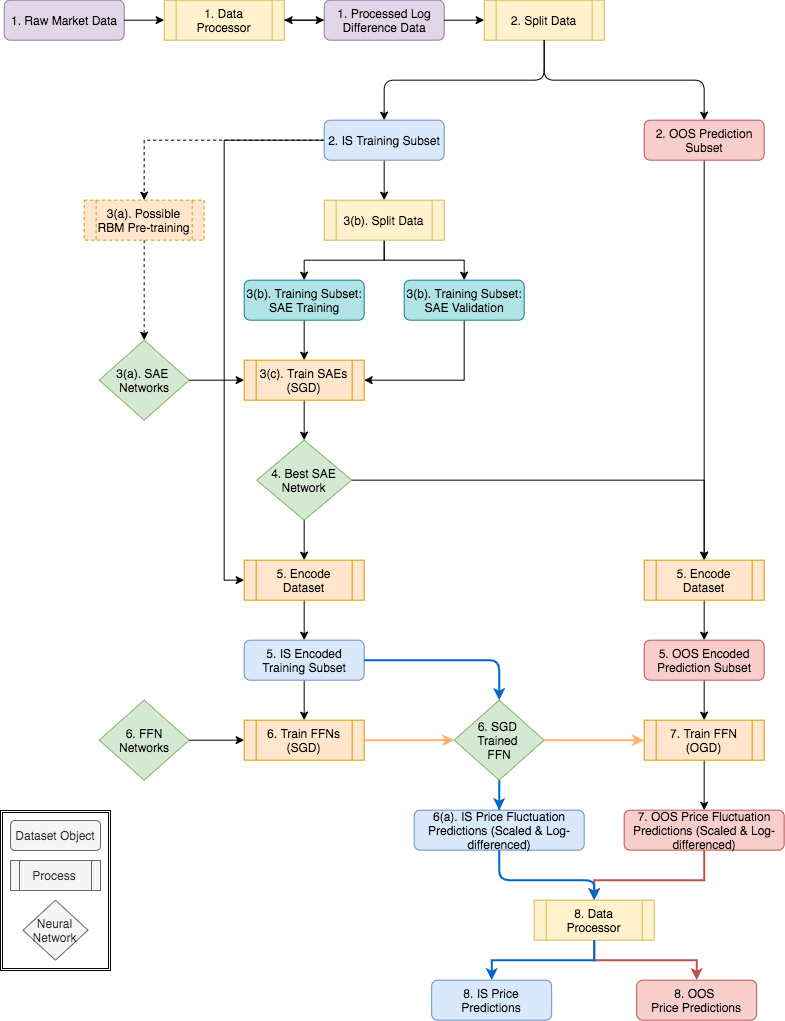
\includegraphics[scale=0.6]{images/process_implementation/process_flow.png}
		\caption[Overall Process Flow Diagram]{Overall Process Flow
		\newline The flow diagram here offers a visual representation of the process set out in Section \ref{imp_fullproc}, with the numbers corresponding to the steps of the process.}
		\label{figure-proc_diagram}
	\end{figure}
	
	\subsection{Parameter Space Exploration}\label{proc_parameters}
	
	The parameter space is explored using a phased grid search approach. For each stage, the relevant parameters are specified as a set of values (or one, if so chosen), and all sets are then used to generate the full combinatorial space, such that each possible combination of the specified parameters is tested.
	
	\begin{enumerate}
		\item \textbf{Stage 1:} The data configuration (i.e. data windows, prediction point, scaling, data split points) as well as the SAE configuration (network size, learning rates, learning optimization parameters, SGD epochs) are set in Stage 1 and used to train the SAE networks.
		\item \textbf{Stage 2:} The preferred SAEs are chosen from Stage 1 manually, and determine the data configuration used for Stage 2. These are then used to encode the datasets, which will be used for FFN training. The FFN SGD and OGD parameters are set in this stage (network size, learning rates, SGD epochs etc.), and will be combined combinatorially with the SAEs that were chosen for testing as well.
	\end{enumerate}
	
	\subsection{Reproducibility}\label{proc_reproducibility}
	
	Reproducible results were ensured with the use of set random data seeds and a Mersenne Twister pseudorandom number generator. Each SAE training process is initialized with a dataseed which is recorded in the \texttt{dataset\_config} schema (see Section \ref{Software} for more details). These are propagated through to the FFN training, such that any of the results presented could be reproduced using the data seeds and configurations noted in Appendix \ref{appendix_configs} (which are all detailed in the relevant figure captions as well).
	
	\subsection{Synthetic Data}\label{proc_synthetic}
	
	The use of synthetic GBM generated data offers a way of exploring the parameter space without running configuration experiments on the actual data, which might then raise the probability of backtest overfitting. The synthetic data has enough similarity that it can allow a broad exploration to get ideas of optimization usage and parameter choices. This is an appealing option in light of the concerns around increasing the number of particularly poor performing networks when it comes to calculating PBO, as discussed in Section \ref{results_pbo}. That said, there are characteristic differences between GBM generated data and actual financial time series. With these in mind, the results section will make comparisons of the two in order to offer a sufficient understanding for when synthetic data can be relied upon to guide future training.\newline
	
	The process for generating synthetic data is detailed in Algorithm \ref{algo_brownianmotion} (Section \ref{Data}).
	
	\subsection{Data Preparation}\label{proc_dataprep}
	
	The full dataset goes through several steps of pre-processing - these are covered in more detail in Section \ref{data_processing}, though the steps are included below.
	
	\begin{enumerate}
		\item The data is processed into day to day log fluctuations (see equation \eqref{eq_logdiff}).
		\item At each time point, rolling historic fluctuation summations are calculated (e.g. the past 1, 7 and 30 days, see equation \eqref{eq_price_agg_past}).
		\item At each time point, rolling future fluctuation summations are calculated (e.g. the next 5 days, see equation \eqref{eq_price_agg_future}).
		\item The dataset is truncated to only include points with all aggregations or predictions available.
		\item The dataset undergoes scaling - the different functions are detailed in Section \ref{data_scaling}, though Limited Normalization (as per equation \eqref{eq_ltd_normalize}) was used for most of the results produced.
	\end{enumerate}
	
	\subsubsection{Data Window Aggregations} The time aggregations were chosen according to domain knowledge - it is expected that prices may move in daily, weekly, fortnightly, monthly and quarterly patterns as trading is actioned by day traders such as speculators to institutional investors such as mutual funds. Indeed, it can be shown that markets can be modelled such that they are hierarchical in space and time, with actors at different hierarchical levels within the market interacting under different causative structures \citep{Wilcox}. The effect is such that price trends and patterns can be expected to exist in time at multiple levels, with price being set as an emergent property of these hierarchies. Taking this into account, variations of 1, 5, 10, 20 and 60 working days were considered throughout the configuration tests, in the following combinations:  
	\begin{enumerate}
		\item Horizon Tuple 1: [1, 5, 20],
		\item Horizon Tuple 2: [5, 20, 60], and
		\item Horizon Tuple 3: [10, 20, 60].
	\end{enumerate}
	~\\
	The calculations for the aggregated values can be seen in equations \eqref{eq_price_agg_past} and \eqref{eq_price_agg_future}.
	
	\subsubsection {Point Predictions} Various configurations were tested in terms of the historic summations used, while the fluctuation predictions were set at 5 days. It's worth noting that the prediction horizon is configurable, and in the case of implementing a more complex trading strategy, one would likely choose to predict multiple points across the horizon in order to to develop a distribution. In this case, the MMS was kept purposefully simple, and so didn't warrant the more intensive implementation. \newline
	
	One point of concern is that point predictions at 5 days in advance could open the process up to aliasing error, as it is unlikely to be predicting at the Nyquist frequency, and may end up fitting to the band ripple rather than the underlying signal. Conversely, 1 day predictions for closing price might offer a high degree of accuracy, but are not practical for trading due to market auction and bidding structures. The system implementation veered on the side of practicality in this case, and was configured for longer term predictions despite the risk of aliasing. While some of the configurations were run with 2 day predictions, it was seen that once costs were considered it was difficult for even the benchmark to produce desired P\&L figures and so a 5 day prediction was implemented in subsequent tests.
	
	
	
	\subsubsection {Scaling} When testing the two limited scaling methodologies, standardization and normalization, it was found that the results for standardizing were significantly worse than normalization (discussed in Section \ref{results_finance_data}). Outliers in price fluctuations and changing variance through time (which is not captured effectively through the limited variation) resulted in a less informative representation and worse performance of the FNN models which can be prone to error maximisation. As a result of this, the limited normalization process was used for most of the tests run. It's worth noting that an implementation which incorporates processing of the data through the Error Function in order to reduce the impact of outliers would likely prove a worthwhile endeavour, and could be easily swapped in due to the systems modularity.\newline
	
	The implementation for ``Limited Normalization'' can be seen in equation \eqref{eq_ltd_normalization}.
	
	\subsection{Data Segregation}\label{proc_dataseg}
	
	Once processed, the dataset is split into 2 portions: 
	\begin{enumerate}
		\item Training: The first set is used for the SAE training, as well as the initial SGD training on the predictive FFN network. This is the IS dataset and is used as what would typically be the historical training set.
		\item Prediction: The second set is used only for the OGD training in order to generate returns from the predictive network. This is the OOS dataset and is used as what would typically be the testing / validation set.
	\end{enumerate}
	
	The predictions from both the Training and the Prediction sets are used by Bailey's CSCV method to assess overfitting (the use of the CSCV technique negates the need for a hold-out portion of the dataset \citep{BailyPBO}), however only the OOS prediction returns are used in order to assess DSR or model P\&L figures and performance. \newline
	
	In this case, a simple split point of 60:40 was chosen for the Training and Prediction sets, respectively. In a more restrictive case, where there is less data to work with, it would be advised to consider a method such as MinBTL as developed by \citet{BaileyBTL} and the estimated number of configurations to be tested in order to decide an appropriate split point.
	
	\subsection{Unsupervised Learning: SAE Training}\label{proc_sae}
	
	The Training dataset is used to train the AutoEncoder network using either RBM pretraining or weight initialization algorithms and SGD training, as defined in Section \ref{imp_SAE}. The Training portion of the dataset, as noted in Section \ref{proc_dataseg}, is itself split up into a training and validation set for the SAE. The efficacy of the SAE on the validation set is required in order to determine which networks to choose for subsequent steps in the process. The full testing process here will rely on a generated set of best SAE networks at each encoding layer size, to be used for FFN training and prediction (chosen by a minimum MSE score). The benefit of the modularised system is emphasised here, as the SAE training will not suffer from limitations due to backtesting considerations: any amount of configurations or processes can be tested for feature extraction without concern. \newline
	
	Once the SAE networks have been defined and chosen, they can be used to reprocess both the Training and Prediction datasets such that the input is encoded, and the output is as before. These encoded datasets can then be used for the following steps in the process. \newline
	
	In a productionized system, where data is updated daily, there would be a set period after which the SAE network would be retrained to reflect more recent data. This step was not deemed necessary at the outset of developing this process, but results detailed in Section \ref{results_oos_pl} suggest that it is an important implementation step.\newline
	
	\subsection{Supervised Learning: Prediction Network Training}\label{proc_predictionnetwork}
	
	Typically, the SAE and predictive network might be presented as one and the same, however in the process presented we are able to separate the two and optimise for feature extraction prior to training for predictions. Having done so, the datasets can have their input encoded, but retain the same output. The predictive network is then trained using the Training set, as detailed in Section \ref{imp_backprop}. There's no requirement to validate this part of the training, so the dataset is not split into subsets as it was for SAE training. \newline
	
	Once the predictive network is trained, the OGD process (as per Section \ref{imp_sgd}) is run through the encoded Prediction dataset in order to generate the predictions for the assets prices that the model produces - thus emulating what would have occurred in a live environment. \newline
	
	\subsection{Price Reconstruction}\label{proc_precerecon}
	
	In the interest of more interpretable results for figures such as P\&L, the prices fluctuations for both IS and OOS predictions are re-scaled back to their original price fluctuation predictions using the reverse scaling detailed in Section \ref{data_reverse_scaling}. These prices are then reconstructed using equation \eqref{eq_price_recon}, such that they represent a predicted future price of the asset which can then be used by the MMS. It's worth nothing that the price reconstruction applies the predicted fluctuation to the known original price, such that it would represent a system that is run daily, rather then a system that is making rolling predictions over a period of time. 
	
	\subsection{Money Management Strategy}\label{proc_mms}
	
	The MMS, as described in Section \ref{imp_mms}, takes a proof of concept approach to the system being investigated. It is a simple long strategy with a set liquidation point, and no notable refinement. The naive approach is taken purposefully here, so as not to bias the perspective of the system as a whole by the effects of an impactful trading strategy. A more effective trading strategy would incorporate a shorting side as well, though ultimately this is not necessary in order to obtain a necessary indication of efficacy for the system (and conceptually, a consistently losing long strategy would be of interest in any case).  \newline
	
	It is important, in the interest of effective optimization and development, that the pattern recognition in the prediction portion of the system is not tightly coupled with making it profitable. With this in mind, the modularity of the system is continued, with a distinct separation between the prediction signal and the MMS implementation which relies only on the predicted prices of each stock for a time point. The comparisons for the MMS are made against a benchmark of the same MMS, but with perfect information. This allows an indication for how effective the prediction system is (and need be) in order to generate comparable returns. \newline
	
	An effective production trading strategy would be likely to include stop losses or pyramiding stop losses for effective P\&L optimization. An ideal implementation, and possible area for further work, would include an MMS strategy where the bands for this are defined using a machine learning technique (rather than being chosen from domain knowledge or heuristics).\newline
	
	The calculated variables used by the MMS are fully detailed in Section \ref{imp_mms}.
	
	\subsection{Probability of Backtest Overfitting}\label{proc_cscv}
	
	The CSCV and PBO parts of the system are essentially just an implementation of Algorithm \ref{algo_cscv} detailed in Section \ref{imp_cscv}, though with a somewhat novel application to the predictive network and MMS combination. The CSCV process uses the IS and OOS returns from the MMS, which in turn used the prices from the predictions network, which then constitutes the $M$ matrix used by the algorithm. Conceptually, the whole system comes into place here, as the results from the CSCV process are now indicative of not only backtest overfitting in the trading strategy, but also in the prediction network and without having to consider the impact of the many configuration tests for feature extraction.
	
	\subsection{Deflated Sharpe Ratio}\label{proc_dsr}
	
	The DSR calculations are a straight forward implementation of the process described in Section \ref{imp_dsr}, with only minor changes from the authors recommendations. Unlike the CSCV process, the DSR calculation only uses returns generated from the predictive model and MMS on OOS data. As with the CSCV \& PBO calculations, the DSR now offers an effective assessment of the experimentations results and their legitimacy. The value of a modularised approach is highlighted again, where the DSR process is not coupled to any aspect of the neural network training.
	
	
	
	
	
	
	
	
	
	
	
	
	
		\newpage
	\section{Software Libraries and Development}\label{Software}
	
	A significant aspect of this dissertation was the implementation of software libraries that fulfilled the criteria of generalised training of neural networks, an implementation of the full process as described later in Section \ref{ProcessOverview}, the creation and management of database records for analysis and an extensive set of diagnostic tools in order to assess performance. This section details the implementation choices as well as the final libraries which were produced.
	
	\subsection{Online Availability}
	
	As per the noted references, all the Julia and Python code developed has been made available via a Github repository and through Zivahub \citep{DCCodeBase}, including the JSE data used to run the trials (see Section \ref{dataset_actual10}). Unfortunately, it was not possible to host the full database that was created, as it had a size of over 60GB.
	
	
	\subsection{Programming Languages}
	
	The libraries developed were primarily written in Julia, a relatively new scientific computing language (initially developed in 2009) \citep{DCRoot, Julia}. The main motivation, both for Julia as a language as well as choosing it for this task, is its efficiency and speed. Julia was created with high performance tasks in mind, and with its use of a Just-In-Time (JIT) compiler, can approach similar benchmarks to C \citep{Perkel}. This stands in stark contrast to some of the more popular analytical languages used, such as R or Python, which often suffer from performance issues. In the context of a project which required extensive processing power, it was natural to prioritize this computational efficiency. \newline
	
	Julia's focus on technical computing is emphasised with its built in support for mathematical and statistical work, composable functional base and dynamic and optional typing schemes. Its ability to fulfil general purpose programming, familiar syntax (which also works effectively for mathematical commands) and its interactive (REPL) command line also make it a practical choice for the task at hand \citep{Perkel}.\newline
	
	SQLite was chosen as the database management language. Relational schemas were a fitting choice for the nature of the data being captured, and SQLite offers a fast, effective and free implementation of SQL.\newline
	
	Python was used only for the DSR algorithm detailed in Section \ref{imp_dsr}, so that the ONC code provided by \citet{PradoDSR} could be used.\newline
	
	\subsection{Data Generation \& Processing}
	
	Data processing libraries were implemented to offer configurable processing for the steps outlined in Section \ref{Data}. The \texttt{DataGenerator} module \citep{DCDataGenerator} implements Geometric Brownian Motion (GBM) generation for a set number of steps and assets with their mean and variances specified. \newline
	
	The \texttt{DataProcessor} module \citep{DCDataProcessor} offers a more extensive set of operations in order to implement the processing laid out in Section \ref{data_processing}. The different scaling techniques (Normalize, Standardize, Limited-Normalize and Limited-Standardize) are implemented, as well as the methods to reverse scaling and reconstruct price predictions to the original format. The log differencing, aggregation of past and future horizons as well as dataset partitioning is also made available here, as per methodologies in Section \ref{Data}. The module also includes dataset encoding through SAE networks, and adding Gaussian noise for the purposes of denoising training, as per Section \ref{imp_denoising}.
	
	
	\subsection{Network Training}
	
	Neural networks were implemented with highly configurable training, such that the parameters are easily specified within Julia types \citep{DCTrainingStructures} and then passed onto the training functions. The parameters are grouped accordingly to the different aspects of the training that they pertain to. \newline
	
	The network structures are easily configurable in terms of layers and layer sizes, as well as having the activation functions specified at each layer (i.e. Linear, Sigmoid, ReLU, LeakyReLU, Softmax, Tanh as described in Section \ref{imp_activation_functions}) \citep{DCActivationFunctions}. The network weight initialization is also specifiable, with the noted initializations in Section \ref{imp_weights} available: Normal Random, Xavier, He and He-Adj \citep{DCInitializationFunctions}.\newline
	
	The Stochastic Gradient Descent (SGD) and Contrastive Divergence-1 (CD-1) learning algorithms, as per Sections \ref{imp_backprop} and \ref{imp_CD}, can be specified according to minimum and maximum learning rates, and learning rate epoch cycles (as per the learning rate scheduling in Section \ref{imp_learning_rate_schedule}). Training length can be specified in terms of maximum training epochs or a custom stopping function, which may rely on the Cost function hitting a particular point (with Mean Squared Error, Cross Entropy Error, Log Likelihood Error being made available \citep{DCCostFunctions}). Learning optimization hyperparameters for L1 Regularization or Denoising are also set here (implemented as per Sections \ref{imp_regularization} and \ref{imp_denoising}). Dataset usage in terms of training / testing splits can also be specified accordingly.\newline
	
	The Online Gradient Descent (OGD) training parameters, as per OGD learning in Section \ref{imp_backprop}, are specifiable through the learning rate and cost functions available.\newline
	
	The \texttt{NetworkTrainer} module \citep{DCNetworkTrainer} then offers 3 primary methods, given the relevant parameter configurations and dataset:
	
	\begin{enumerate}
		\item Train a Feedforward Neural Network, using variance based weight initializations.
		\item Train an SAE, using variance based weight initializations.
		\item Train an SAE, using RBM based pre-training for weight initialization.
	\end{enumerate}
	
	These functions are supported by the following learning algorithm modules: \texttt{SGD} \citep{DCSGD}, \texttt{RBM} \citep{DCRBM}, \texttt{OGD} \citep{DCOGD} and  \texttt{GradientFunctions} \citep{DCGradientFunctions}.
	
	\subsection{Process Implementation}
	
	The process implementation, as described in detail in Section \ref{ProcessOverview}, is largely implemented in the \texttt{ExperimentProcess} module \citep{DCExperimentProcess}.
	
	~\\
	The \texttt{RunSAEConfigurationTest} method uses the \texttt{SAEExperimentConfig} Type to wrap up all necessary configurations and with a passed dataset runs through the following steps:
	\begin{enumerate}
		\item Either generate or process the raw dataset, according to the specified configuration.
		\item Train the SAE, either with RBM or variance based weight initializations.
		\item Pass back the SAE with original and reconstructed testing datasets.
		\item Store the SAE as a bson object to be used later.
	\end{enumerate}
	
	~\\
	The \texttt{RunFFNConfigurationTest} method similarly uses the \texttt{FFNExperimentConfig} Type and a passed dataset to run through the following steps:
	\begin{enumerate}
		\item Either generate or process the raw dataset, according to the specified configuration.
		\item Encode the datasets for the different steps of the process using the specified SAE.
		\item Train the FFN using variance based weight initialization and SGD.
		\item Use the FFN to generate predictions for IS data, reconstruct them and record them in the database.
		\item Train the FFN using OGD on OOS data.
		\item Use the FFN to generate predictions for OOS data, reconstruct them and record them in the database.
	\end{enumerate}
	
	Two further modules allow the exploration of the configuration space, such that diagnostics can be performed on different aspects of the training. 	The \texttt{ExperimentProcessTrainFFN} \citep{DCExperimentProcessTrainFFN} and \texttt{ExperimentProcessTrainSAE} \citep{DCExperimentProcessTrainSAE} modules make use of the \texttt{ConfigGenerator} module \citep{DCGenerator} in order to generate a full grid configuration space for a given range of values for any chosen parameters, as per Section \ref{proc_parameters}. Each of these combination configuration sets is then run as per the processes detailed above, with the various results recorded as usual. 

	\subsection{Process Reproducibility}
	
	As noted in Section \ref{proc_reproducibility}, it was ensured that the full process and results were reproducible. A Mersenne Twister pseudorandom number generator was set with a particular seed, which is recorded in the \texttt{dataset\_config} schema in the database. This seed is propagated through from the SAE training process to the FFN training process. Consequently, any configuration set with the same parameters and random seed can be used to reproduce the results presented in this paper and otherwise.
	
	\subsection{Database Implementation}\label{software_database}
	
	As noted, the database platform chosen was SQLite, with Julia modules handling the creation and management. The \texttt{DatabaseCreator} module \citep{DCDatabaseCreator} easily creates the database, with the schema names and purposes noted in Table \ref{tab_schemas}, using the \texttt{CreateDatabase} function. The full relational schema diagram can also be viewed in Figure \ref{figure-database_schema} in the Appendix. \newline
	
	The \texttt{DatabaseOps} module \citep{DCDatabaseOps} handles the creation of records for these schemas, as well as the writing and reading of bson files which are used to store actual neural networks in the form of the \texttt{FFN} type \citep{DCFFN}.
	
	\subsection{Diagnostic Libraries}
	
	The diagnostic implementations were focused on 2 primary themes: Exploratory Data Analysis (EDA) through the use of visualizations of network results through configuration spaces, and formalised testing in the form of PBO and DSR.\newline
	
	The EDA makes use of the PlotlyJS library \citep{PlotlyJS}, and allows the net performance of any set of networks to be plotted along a particular dimension in their configuration space. In the case of a set of SAE networks, this would typically be the MSE scores, and in the case of predictive FFN networks, this would typically be the P\&L values generated from the MMS. A full list of diagnostic charts can be viewed in Appendix \ref{appendix_diagnostics}. \newline
	
	The CSCV and PBO methodologies can be found in the \texttt{CSCV} module \citep{DCCSCV}, which encapsulates the generation and assessment of the logit distributions, as well as the PBO calculation.
	
	\subsubsection{DSR Libraries}
	
	Unlike the rest of the framework implementation, the DSR process was written in Python \citep{Python}. This was done so the code provided by \citet{PradoDSR} for the ONC algorithm (see Section \ref{imp_onc}) could be used. The \texttt{DSR\_PradoLewis} module \citep{DCDSR_PradoLewis} contains all the python code used which was presented in \citep{PradoDSR}. Modules \texttt{DSR\_dataproc} \citep{DCDSR_Dataproc} and \texttt{DSR\_proc} \citep{DCDSR_proc} contain the code for returns processing and DSR calculations, respectively.
	
	\begin{table}[H]
		\begin{tabular}{|p{0.33\linewidth}|p{0.67\linewidth}|}
			\hline
			\textbf{Schema Name} &\textbf{Description}  \\\hline	
			{configuration\_run} & {The primary record for any trial configuration run.} \\\hline
			{dataset\_config} & {The dataset configuration that may relate to a trial.} \\\hline
			{network\_parameters} & {The network configuration for a trial.} \\\hline
			{training\_parameters} & {The SGD/RBM/CD training configuration for a trial.}  \\\hline
			{epoch\_records} & {Details relating to ongoing training performance for the duration of a trial.}  \\\hline
			{backtest\_results} & {Predictions for IS data made by trial networks after SGD training.}  \\\hline
			{prediction\_results} & {Predictions for OOS data made by trial networks during OGD training.}  \\\hline
			{config\_is\_trade\_returns} & {MMS P\&L observed and return rates for each IS trade for each trial.}  \\\hline
			{config\_is\_trade\_returns\_cost} & {MMS P\&L observed and return rates for each IS trade for each trial, with trading costs applied.}  \\\hline
			{config\_oos\_trade\_returns} & {MMS P\&L observed and return rates for each OOS trade for each trial.}  \\\hline
			{config\_oos\_trade\_returns\_cost} & {MMS P\&L observed and return rates for each OOS trade for each trial, with trading costs applied.}  \\\hline
			{config\_is\_pl} & {The total IS P\&L for a trial.}  \\\hline
			{config\_is\_pl\_cost} & {The total IS P\&L for a trial, with trading costs applied.}  \\\hline
			{config\_oos\_pl} & {The total OOS P\&L for a trial.}  \\\hline
			{config\_oos\_pl\_cost} & {The total OOS P\&L for a trial, with trading costs applied.}  \\\hline
			{config\_oos\_sharpe\_ratio} & {The OOS Sharpe Ratio for each trial.}  \\\hline
			{config\_oos\_sharpe\_ratio\_cost} & {The OOS Sharpe Ratio for each trial, with trading costs applied.}  \\\hline			
			{config\_confusion} & {The percentages of correct trades made for a trial.}  \\\hline
			{clusters} & {The clusters for the trials as determined by the ONC algorithm.}  \\\hline
		\end{tabular}
		\newline\newline
		\caption{Database schema descriptions, as discussed in \ref{software_database}.}\label{tab_schemas}
	\end{table}
	
	\newpage
	\section{Datasets Used}\label{Datasets}
	
	\subsection{Actual Datasets}
	
	Several datasets have been used using JSE closing price relative data for 2003-2018 (more source information and a data snapshot are available in Appendix \ref{appendix_dataset}) \citep{JSEData}. They were processed following the steps set out in Section \ref{Data} and with a 60:40 split on the Training:Prediction datasets.
	
	\subsubsection{``Actual10''}\label{dataset_actual10}
	
	This is the primary closing price dataset that has been used through out the experiment process, which focused on choosing more prominent stocks from multiple sectors. The price fluctuations can be seen in Figure \ref{figure-actual10_prices}.
	
	\begin{table}[H]
		\centering
		\begin{tabular}{|c|c|c|}
			\hline
			\textbf{Code} &\textbf{Company} & \textbf{Sector} \\\hline	
			{AGL} & {Anglo American} & {Resources}  \\\hline
			{BIL} & {BHP Billigton} & {Resources}  \\\hline
			{IMP} & {Impala Platinum Holdings} & {Resources}  \\\hline
			{FSR} & {FirstRand Limited} & {Finance}  \\\hline
			{SBK} & {Standard Bank} & {Finance}  \\\hline
			{REM} & {Remgro Limited} & {Finance}  \\\hline
			{INP} & {Investec} & {Finance}  \\\hline
			{SNH} & {Steinhoff International Holdings} & {Retail}    \\\hline
			{MTN} & {MTN} & {Communication Services}  \\\hline
			{DDT} & {Dimension Data} & {Tech} \\\hline
		\end{tabular}
		\newline\newline
		\caption{Assets in the ``Actual10'' dataset, from 2003-2018. }\label{tab_actual10}
	\end{table}
	
	\subsubsection{``Scaling10''}\label{dataset_scaling10}
	
	 This dataset was used specifically to test scaling techniques, and consisted of the following JSE closing price relatives: ACL, AGL, AMS, AOD, BAW, BIL, BVT, CFR, CRH, DDT. The price fluctuations can be seen in Figure \ref{figure-scaling10_prices}.
	
	\subsubsection{``AGL'' and ``AGL\&ACL''}\label{dataset_agl}\label{dataset_aglacl}
	
	The AGL and ACL data from JSE closing price relatives was used for some limited framework testing. The price fluctuations can be seen in Figure \ref{figure-aglacl_prices}.
	
	\begin{figure}[H]
		\centering
		\textbf{``Actual10'' Price Relatives}
		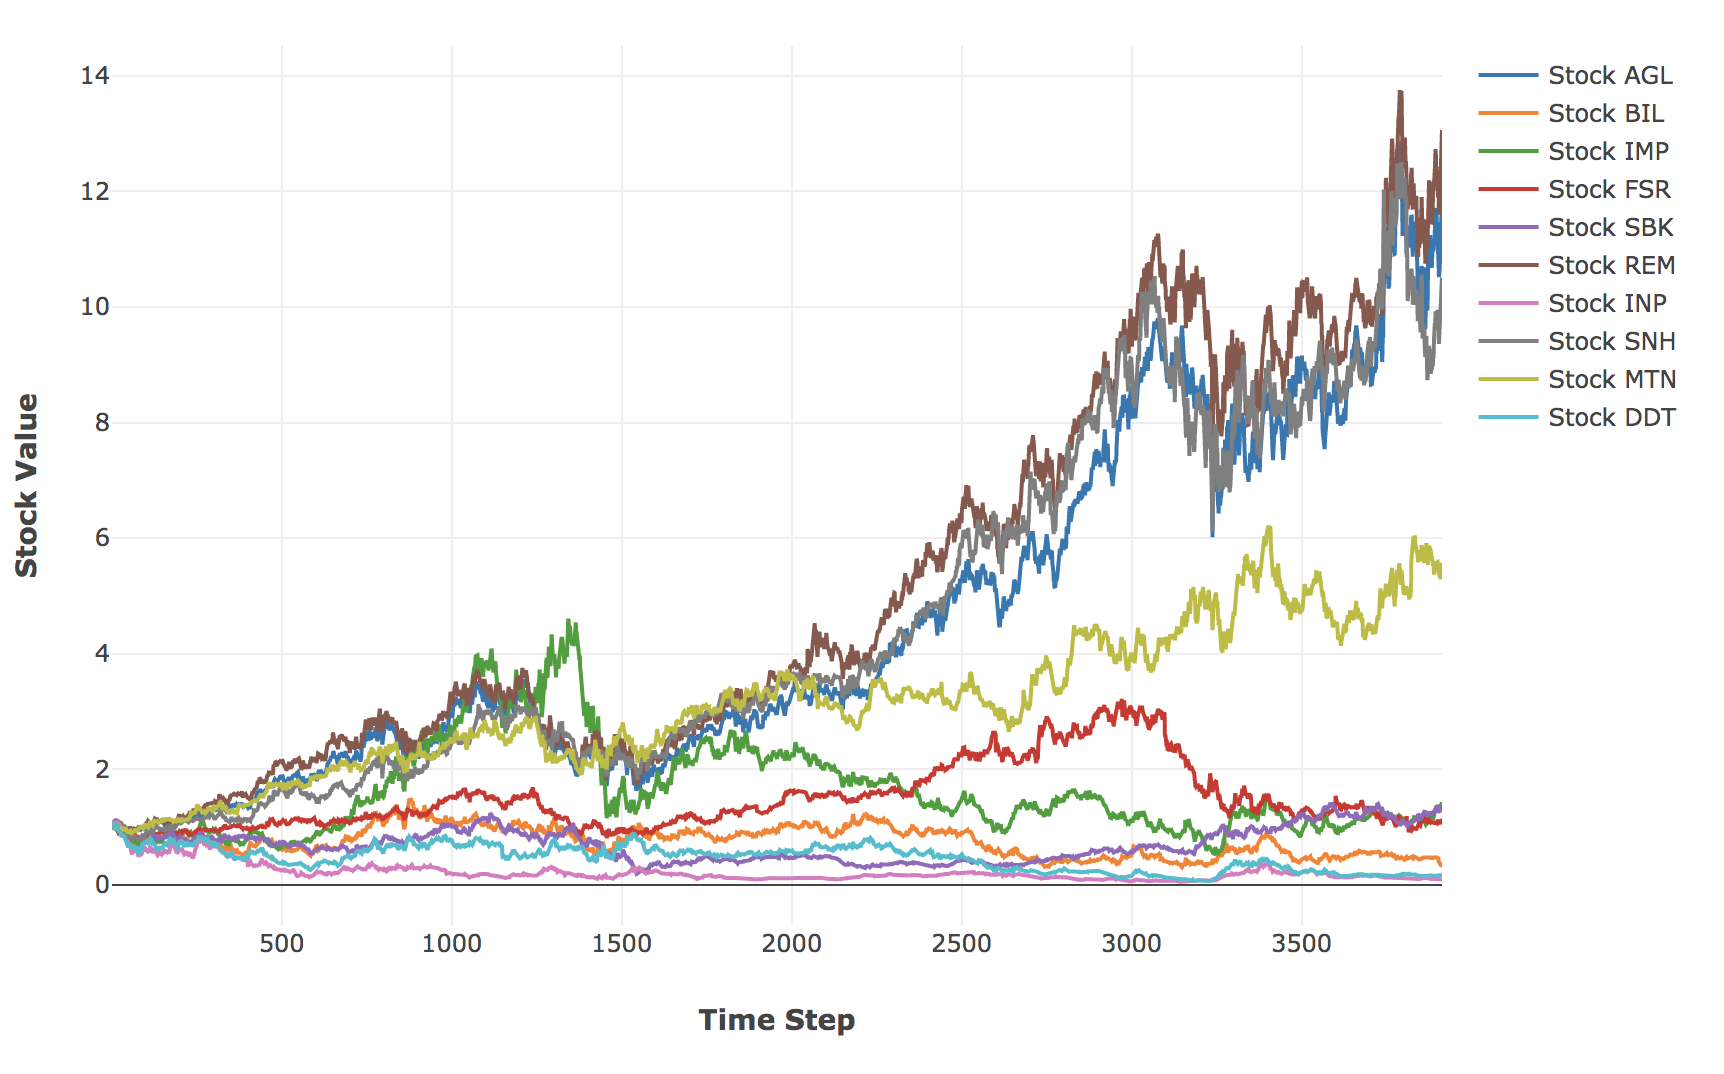
\includegraphics[scale=0.45]{images/results/prices/actual10_prices.png} 
		\caption[``Actual10'' Price Relatives]{The primary dataset for actual price relatives is displayed here, as noted in Table \ref{tab_actual10}. There is a varied collection of behaviours amongst assets, with upwards, downwards and sideways trends over the full period, as well as assets with very high and low variances. The dataset contains assets from most major sectors, and shows some strong correlations amongst groups of assets (e.g. AGL, REM and SNH). }
		\label{figure-actual10_prices}
	\end{figure}
	
	\begin{figure}[H]
		\centering
		\textbf{``Scaling10'' Price Relatives}
		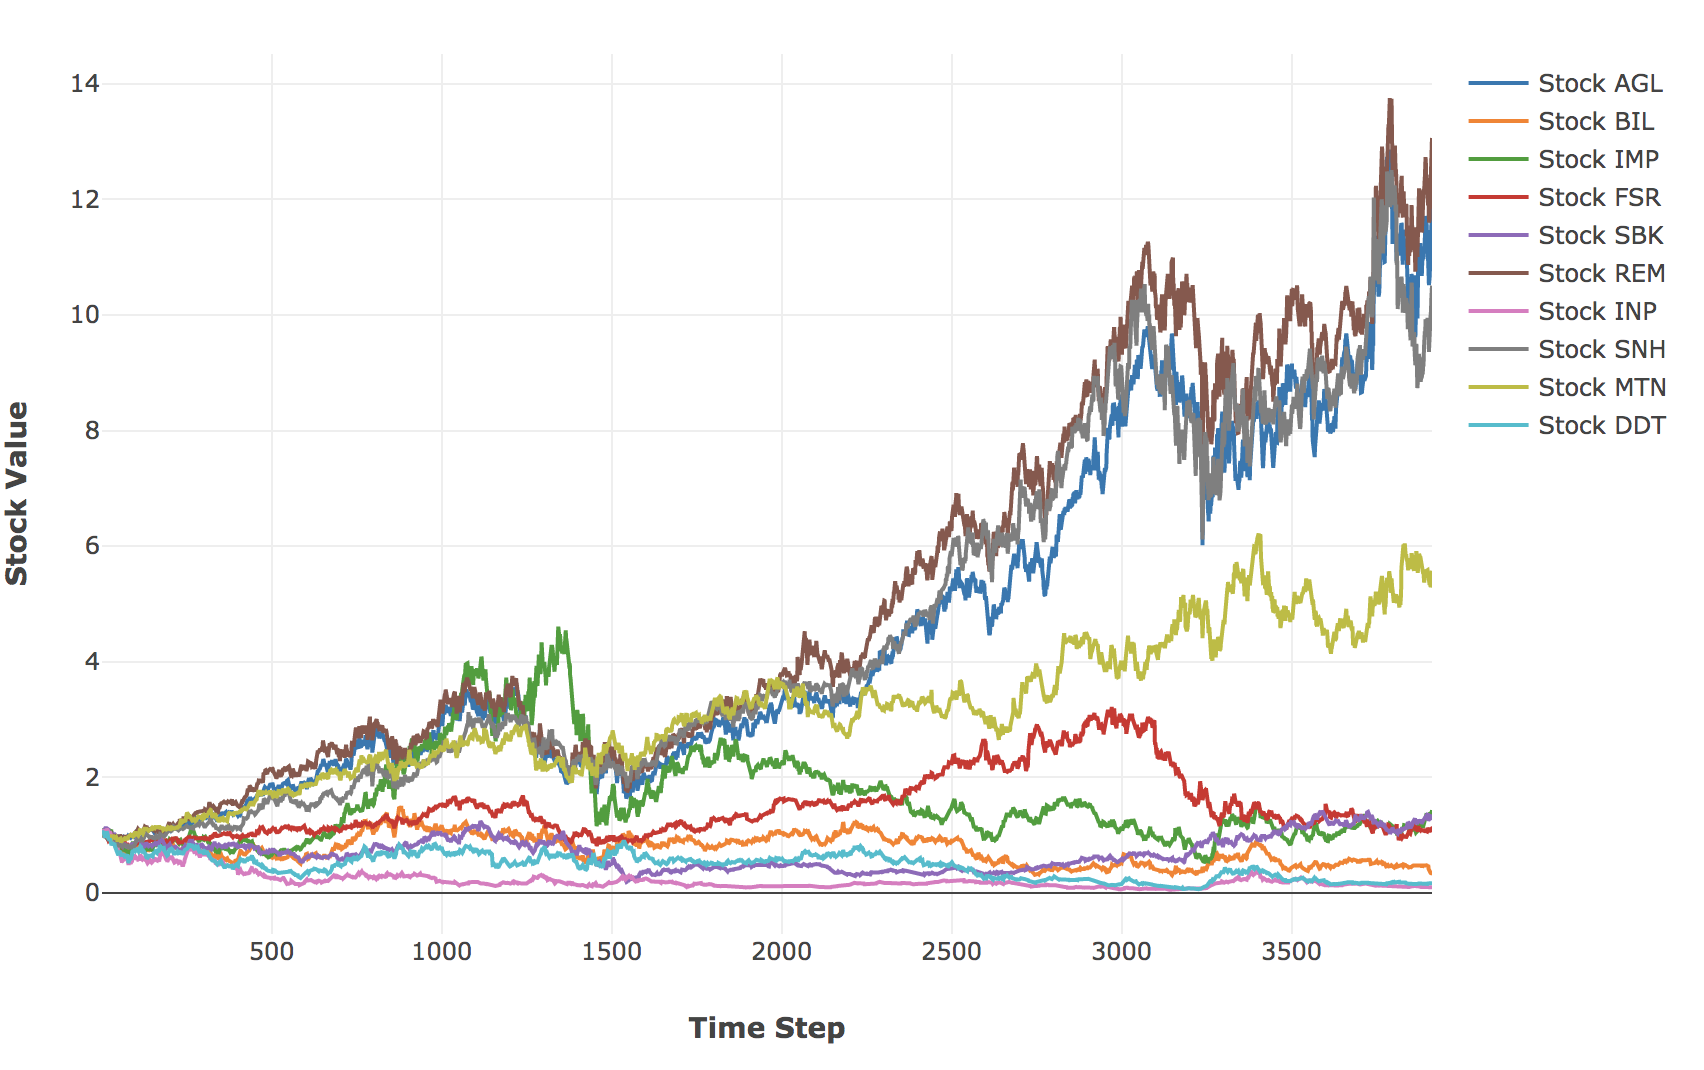
\includegraphics[scale=0.45]{images/results/prices/scaling10_prices.png} 
		\caption[``Scaling10'' Price Relatives]{The figure here shows the prices relatives for the ``Scaling10'' Dataset as detailed in Section \ref{dataset_scaling10}. The group of assets show a wide variety of behaviours, which was appropriate for the testing of training techniques on SAE networks. These results can be seen in Section \ref{results_activations_scaling}.}
		\label{figure-scaling10_prices}
	\end{figure}
	
	\begin{figure}[H]
		\centering
		\textbf{``AGL \& ACL'' Price Relatives}
		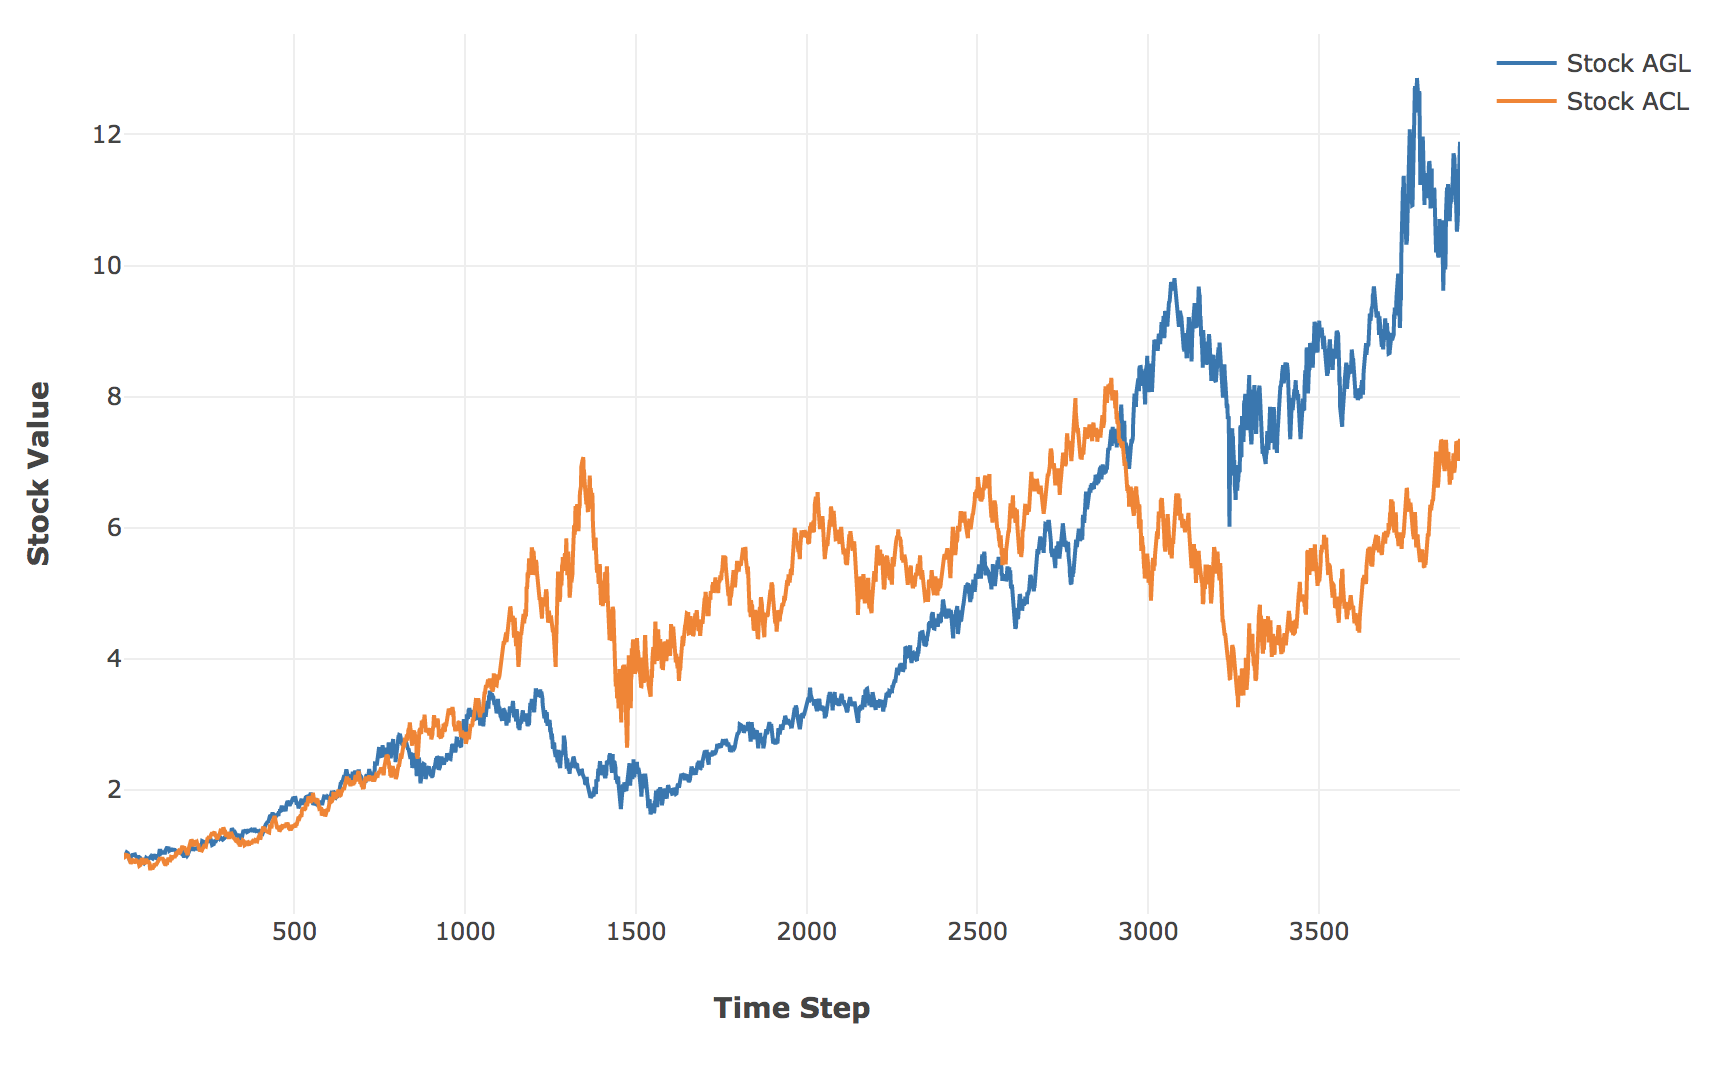
\includegraphics[scale=0.45]{images/results/prices/aglacl_prices.png} 
		\caption[``AGL\&ACL'' Price Relatives]{The figure here shows price relatives for AGL and ACL which make up the ``AGL'' and ``AGL\&ACL'' datasets (\ref{dataset_agl}, \ref{dataset_aglacl}), which were used for some limited testing (e.g. scaling as in Figure \ref{figure-actual_mse_scaling} and initializations as in Figure \ref{figure-mse_init}).}
		\label{figure-aglacl_prices}
	\end{figure}
	

	
	
	\subsection{Synthetic Datasets}
	
	Data was generated and scaled, as per the methods detailed in Sections \ref{data_synthetic} and \ref{data_scaling}. The sets were generated with the following configurations, each for 5000 timesteps and with a 60:40 split on the Training and Prediction sets.
	
	\subsubsection{``Synthetic6''} \label{dataset_synthetic6}
	
	The Synthetic6 dataset was configured to represent a combination of upwards, downwards and sideways Trends, each with high and low variance variations.
	
	\begin{table}[h]
		\centering
		\small
		\begin{tabular}{|c|c|c|c|}
			\hline
			\textbf{Trend Category} &\textbf{Variance Category} & \textbf{Trend Mean} & \textbf{Variance}\\\hline	
			{Strong Upward} & {High} & {0.9} & {0.5} \\\hline
			{Strong Upward} & {Low} & {0.9} & {0.2} \\\hline
			{Upward} & {High} & {0.05} & {0.4} \\\hline
			{Upward} & {Low} & {0.05} & {0.1} \\\hline
			{Strong Downward} & {High} & {-0.8} & {0.55} \\\hline
			{Strong Downward} & {Low} & {-0.8} & {0.15} \\\hline
		\end{tabular}
		\newline\newline
		\caption{Assets in the ``Synthetic6'' dataset, as detailed in Section \ref{dataset_synthetic6}.}\label{tab_synth6}
	\end{table}
	
	\subsubsection{``Synthetic10''}\label{dataset_synthetic10}
	
	The Synthetic10 dataset was configured to represent a wide array of behaviours, including very high (positive and negative) mean stocks, as well as much lower mean stocks (which may be more representative of typical behaviour). These were chosen to make sure the network learning is able to differentiate and correctly learn across different asset categories.
	
	\begin{table}[H]
		\centering
		\small
		\begin{tabular}{|c|c|c|c|}
			\hline
			\textbf{Trend Category} &\textbf{Variance Category} & \textbf{Trend Mean} & \textbf{Variance}\\\hline	
			{Strong Upward} 		& {High} & {0.9} & {0.5} \\\hline
			{Strong Upward} 		& {Low} & {0.7} & {0.2} \\\hline
			{Upward} 					& {High} & {0.05} & {0.5} \\\hline
			{Upward} 					& {High} & {0.05} & {0.4} \\\hline
			{Upward} 					& {Low} & {0.04} & {0.1} \\\hline
			{Sideways} 					& {Low} & {0.02} & {0.15} \\\hline
			{Sideways}					& {Low} & {0.01} & {0.05} \\\hline
			{Downwards}				& {Low} & {-0.1} & {0.2} \\\hline
			{Strong Downward} 	& {Low} & {-0.4} & {0.15} \\\hline
			{Strong Downward}	& {High} & {-0.8} & {0.55} \\\hline
		\end{tabular}
		\newline\newline
		\caption{Assets in the ``Synthetic10'' dataset, as detailed in Section \ref{dataset_synthetic10}.}\label{tab_synth10}
	\end{table}
	
	\begin{figure}[H]
		\centering
		\textbf{``Synthetic6'' Price Relatives}
		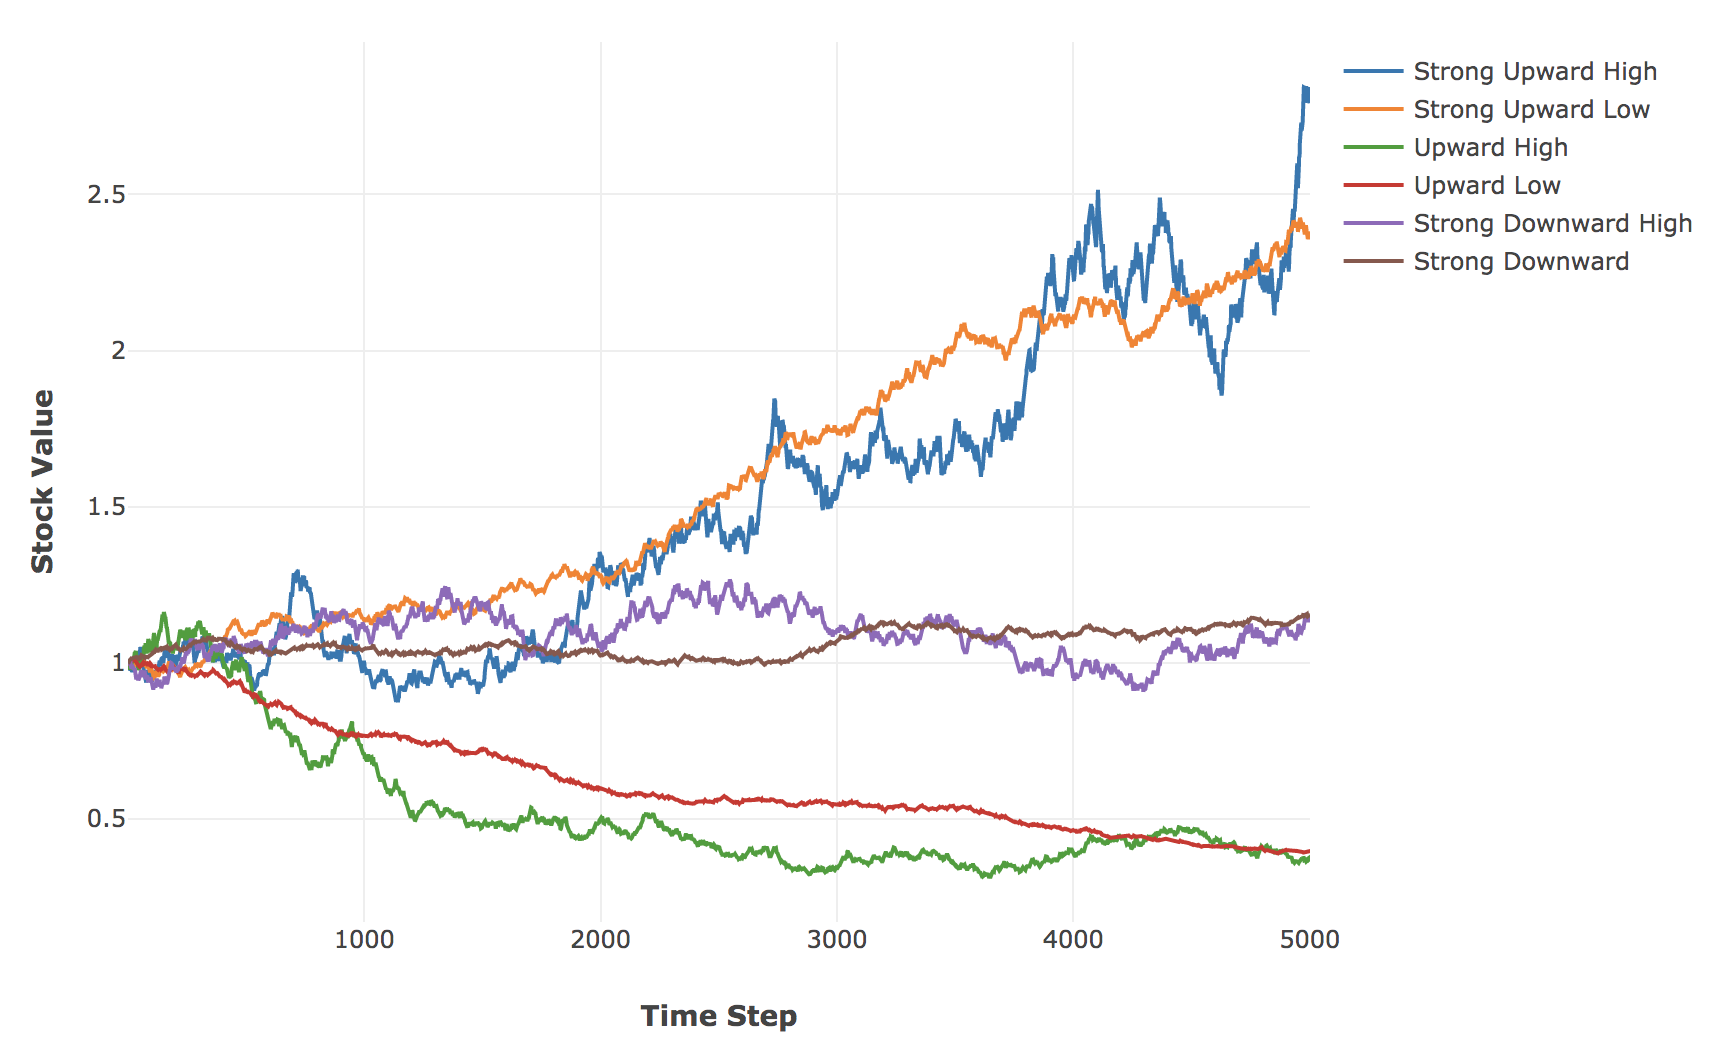
\includegraphics[scale=0.45]{images/results/prices/synthetic6_prices.png} 
		\caption[Synthetic6 Price Relatives]{This figure shows the price relatives for the Synthetic6 dataset (Section \ref{dataset_synthetic6}), generated for 5000 days and with the attributes in Table \ref{tab_synth6}. Assets were generated for high and low variances with upwards, downwards and sideways trends.}
		\label{figure-synthetic6_prices}
	\end{figure}
	
	
	
	\begin{figure}[H]
		\centering
		\textbf{``Synthetic10'' Price Relatives}
		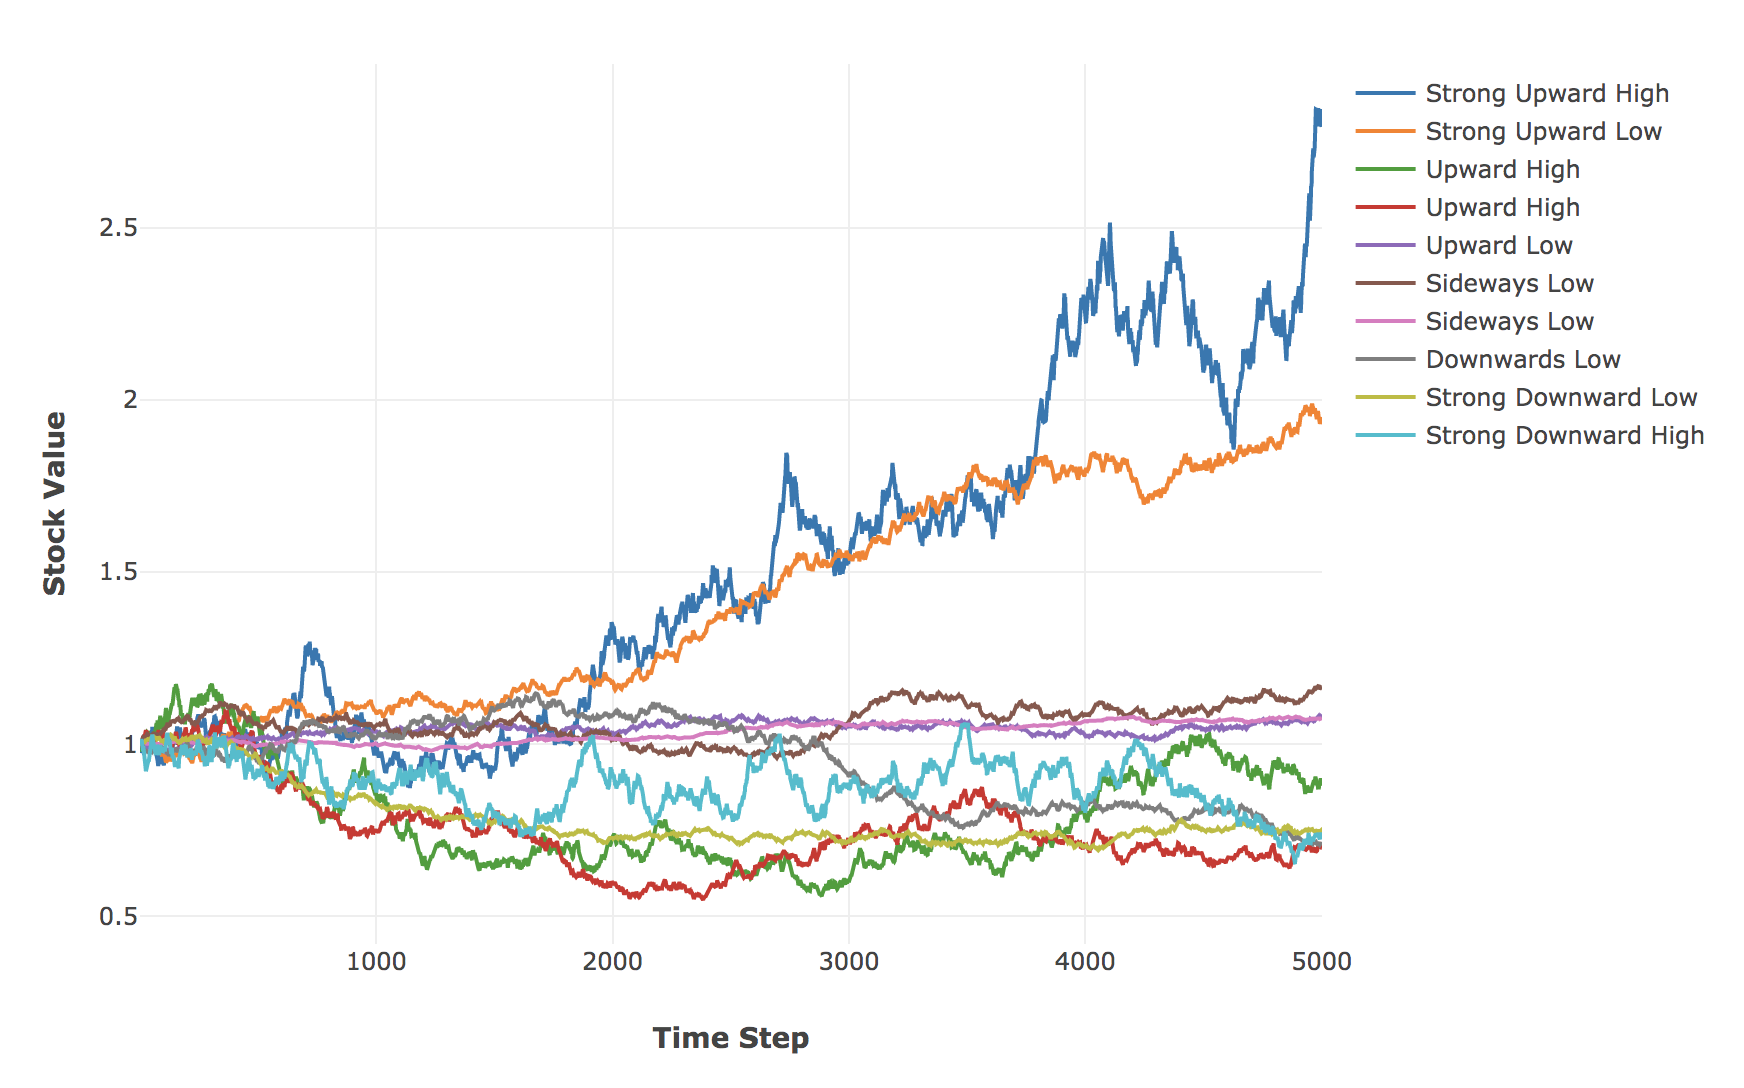
\includegraphics[scale=0.45]{images/results/prices/synthetic10_prices.png} 
		\caption[Synthetic10 Price Relatives]{This figure show the price relatives for the Synthetic10 dataset (Section \ref{dataset_synthetic10}), generated for 5000 days and with the attributes in Table \ref{tab_synth10}. A wide range of means and variances were chosen, such that the data might be representative of a non-synthetic dataset.}
		\label{figure-synthetic10_prices}
	\end{figure}
	

	
	
	
	
	
	
	
	
	
	\newpage
	\section{Results}\label{Results}
	\subsection{Introduction}\label{results_into}
	
	This section offers a full discussion of the results seen at all stages in the framework, providing numerous takeaways both in terms of technical training as well developing a perspective on the phenomenology of financial markets, and how these influence mechanistic learning approaches to pattern prediction. \newline
	
	\textbf{OOS P\&L:} Section \ref{results_oos_pl} discusses the primary determinants of OOS P\&L seen in actual data results, covering data horizon aggregations, SAE feature reduction and the OGD learning phase. It's shown that data horizon aggregations form the primary determinant of the prediction strategies learnt, and that SAE networks learn different classes of features according to the encoding size (which may differ in suitability for different prediction strategies). These are both considered in the context of the online OOS learning, which proves to be critical in effective learning. This is expanded on in Section \ref{results_data_hist}, which shows the negligible impact of extensive training on historical data, noting that reducing training epochs and datasets has limited effect, and that the online learning phase is most impactful for OOS P\&L. \newline
	
	\textbf{Network Initializations:} Section \ref{results_init} discusses network weight initialization techniques, noting their importance in context of financial time series where the value of extensive batch training has been shown to be of limited value (or even detrimental to performance).\newline
	
	\textbf{Synthetic Data OOS P\&L:} Section \ref{results_synth} discusses the nature of Synthetic data, and how it differs in the key OOS determinants. The fundamental differences in data distributions result in P\&L performing better over longer data horizons (which is not definitive in actual data), and less complex features being learnt in SAE networks.\newline
	
	\textbf{Complexity:} The complexity of actual financial time series is discussed further in Section \ref{results_finance_data}, where results for data scaling and SGD learning optimizations are shown to be affected be the unstable nature of dynamics in financial markets.\newline
	
	\textbf{Network Configuration:} Section \ref{results_network} gives an overview of the more typical network training components such as layer sizes and activation functions.\newline
	
	\textbf{Trial Validation:} The financial returns and Sharpe ratios from the prediction networks, as used by the MMS, are discussed in Section \ref{results_mms} with overall distributions shown with the relative benchmark. These results are validated, showing a low likelihood of backtest overfitting in Section \ref{results_pbo}, and showing a confidently positive Deflated Sharpe Ratio in Section \ref{results_dsr}.  \newline
	
	\textbf{Synthetica Data Assessment:} Lastly, Section \ref{results_synth_summary} summarises the results presented for synthetic data throughout the framework, and notes its limited value in assessing behaviours for actual data.
	
	\subsubsection{Technical Notes}
	
	While the predictive networks are trained using an MSE loss function, the performance will mostly be reported on according to the P\&L they were able to achieve through the MMS. Looking at Figure \ref{figure-ogdmse_pl}, we can see that while there is a strong correlation between predictive accuracy and P\&L achieved, it is not absolute and there are many ``worse'' configurations according to OGD MSE which have higher P\&L. This is due in part to OGD's potential to oscillate wildly in the beginning of training while it adjusts, and also representative of lower variance models being able to achieve competitive P\&L. Also, in consideration of the task at hand, P\&L is the primary metric of interest and so is a sensible analysis choice. It is worth noting though that this P\&L is a relative unit measurement, rather than a particular currency (as noted in Section \ref{data_prices}), and that the MMS, as described in Section \ref{imp_mms}, only trades 1 stock unit at a time, and so any P\&L figures are relative indications rather than absolute limits. It is also usually reported without capital and trading costs (as per equation \eqref{eq_capital_costs}) applied, though these costs are taken into account for the PBO and DSR validations. \newline

	The results for synthetic data are compared against actual data when appropriate, such that it might guide when synthetic data can and should be used for parameter space exploration (as discussed in Section \ref{proc_synthetic}). These results are discussed more completely in Sections \ref{results_synth} and \ref{results_synth_summary}.\newline

	Sample sizes for some configurations may differ greatly across results (particularly as results are aggregated across training sets and phases), though these are noted in the figures as well as the configurations in the appendix.\newline
	
		\begin{figure}[H]
		\textbf{OGD MSE vs. P\&L}
		\centering
		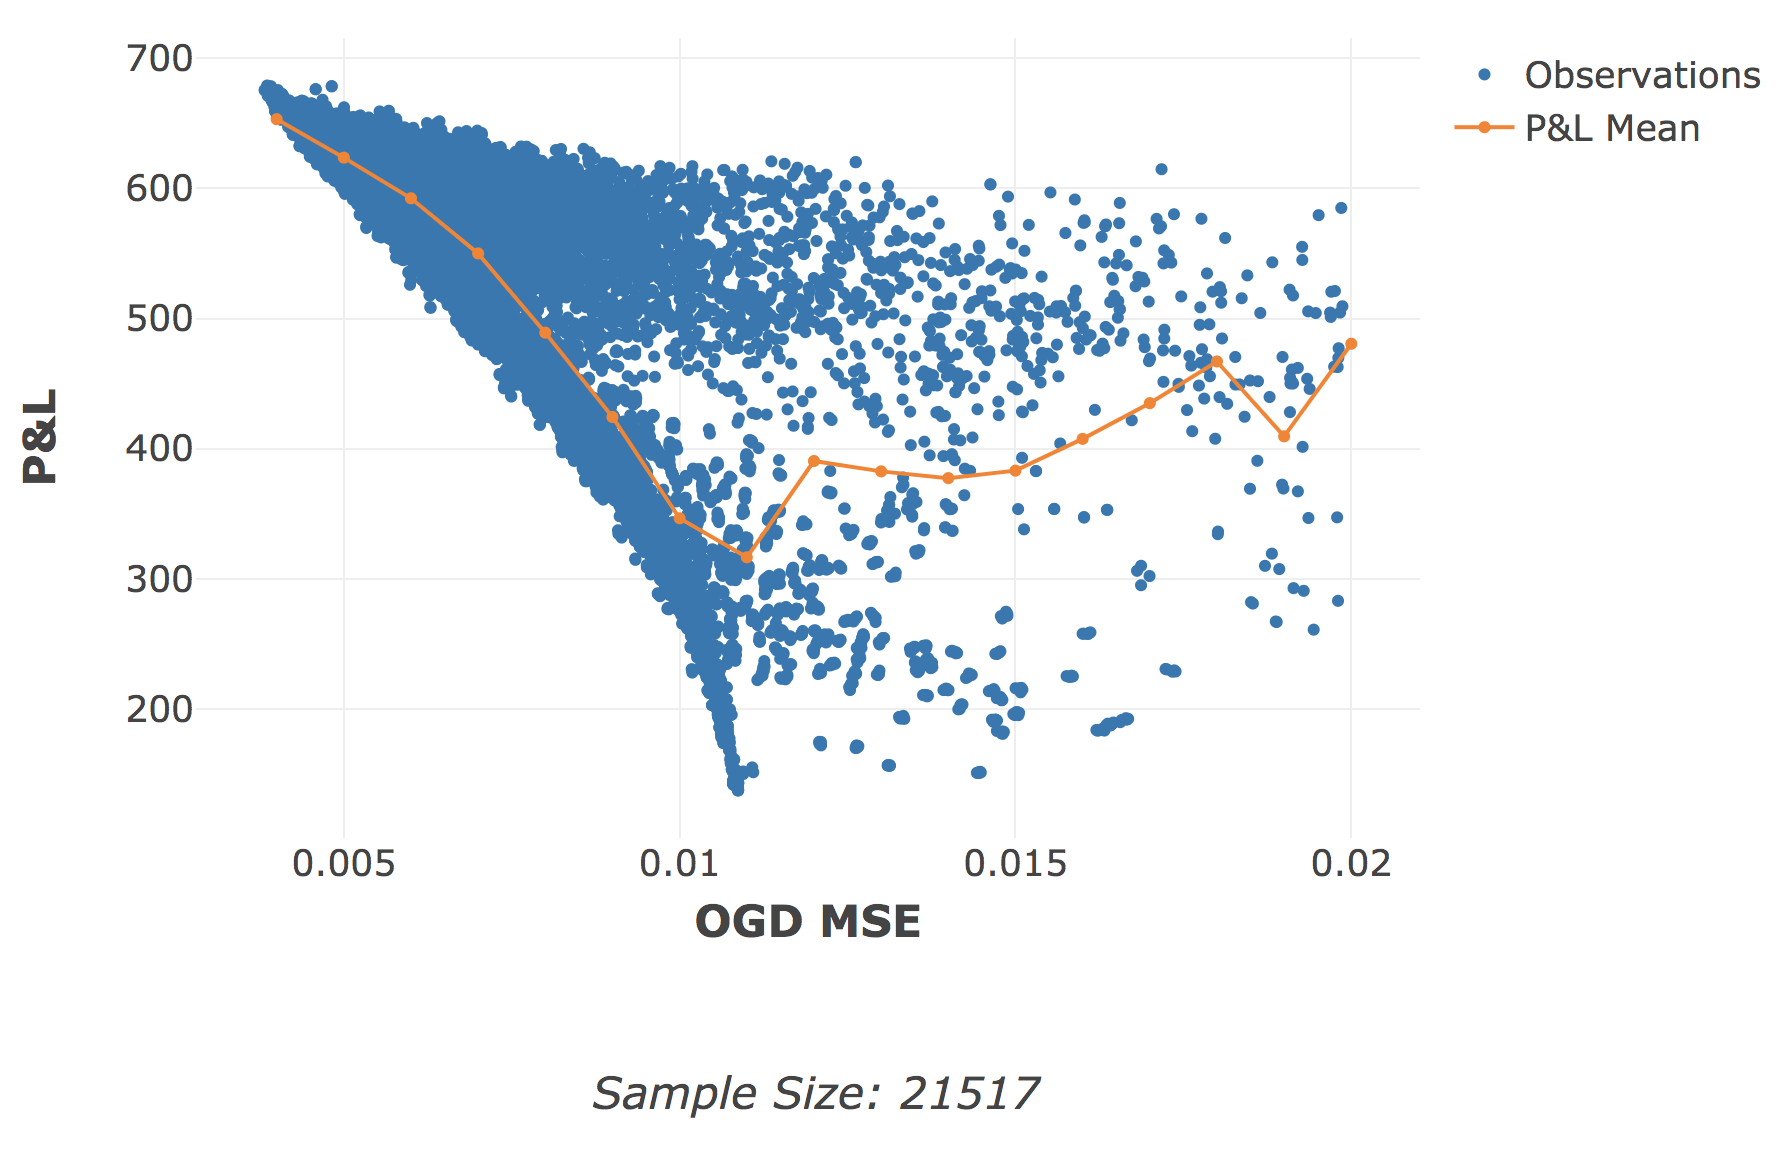
\includegraphics[scale=0.45]{images/results/intro/ogdmse_pl.png}
		\caption[OGD MSE vs. OOS P\&L]
		{Dataset: Actual10 (\ref{dataset_actual10}) ; Configuration 11 (\ref{config11}) \&  Configuration 16 (\ref{config16}) \newline 
			The figure here shows the paired OGD MSE score and OOS P\&L achieved for all 22248 trials run, excluding networks with null returns (a result of exploding gradients). There is a very strong correlation with $\rho = -0.74$, indicating the relationship of P\&L increasing as OGD MSE decreases (or, as predictive accuracy increases). As can be seen however, there are still many configurations which outperform in P\&L despite having a worse OGD MSE score (reasons are noted above in Section \ref{results_into}). As a result, and with the end goal in mind, P\&L is chosen as the primary reporting assessment metric for the analyses on predictive networks. }
		\label{figure-ogdmse_pl}
	\end{figure}
	
	\newpage
	\subsection{Primary Determinants of OOS P\&L}\label{results_oos_pl}
	
	Our initial expectations were that the IS batch training using SGD for the predictive network would improve OOS P\&L performance. Theoretically, the training on historical data might prime the network for predicting future data. However, we found that the effects of IS training had limited effect. This limited effect highlights the complexity and dynamic nature of financial time series, where past relations and behaviours are not necessarily indicative of present state. These issues are discussed extensively in Section \ref{results_data_hist}, however the follow through is that the primary determinants of OOS P\&L are those which are present in the OGD (OOS) learning phase: the OGD learning rate, the data horizon aggregations and the SAE feature reduction.\newline
	
	\subsubsection{Effects of Data Horizon Aggregations}
	
	Input data was scaled to 3 different configurations to assess the effects of shorter and longer data horizons. Both SAE MSE and predictive P\&L measures were used to assess performance. The configurations tested (in trading day window periods) were:
	
	\begin{enumerate}
		\item Horizon Tuple 1. [1, 5, 20],
		\item Horizon Tuple 2. [5, 20, 60], and
		\item Horizon Tuple 3. [10, 20, 60].
	\end{enumerate}
	
	By way of example, using the 3rd configuration: the implementation of this is such that at each time point considered, the log differenced changes for the past 10, 20 and 60 days are available for each asset. This is described more extensively in Section \ref{Data}.\newline
	
	We found that the predictive strategies learnt by the networks were determined by the data horizon aggregations chosen: predictions using short term fluctuations (with horizons of [1, 5, 20] days) and predictions using long term trends (with horizons of [5, 20, 60] or [10, 20, 60]). The differentiation between these groups is shown more robustly in Section \ref{results_dsr}, where it is determined to be the primary clustering attribute for trade correlations.  We found that using short term fluctuations is a less reliable strategy, with higher variance in the returns delivered. However, the strategies using short term fluctuations also deliver the highest P\&L and Sharpe ratios. The P\&L comparison can be seen below in Figure \ref{figure-actual_aggregation_pl}. \newline

	We also found that the horizons impact the ability of the SAE network to reconstruct the aggregations. Lower variance in the shorter horizon aggregations result in easier replication, while longer horizons are more difficult (as indicated through MSE scores). The reproduction differences can be seen below in Figure \ref{fig_data_sae_actual}.	
	
	
	\begin{figure}[H]
		\centering
		\textbf{SAE MSE Scores by Data Aggregations}
		\begin{subfigure}{.99\textwidth}
			\centering 
			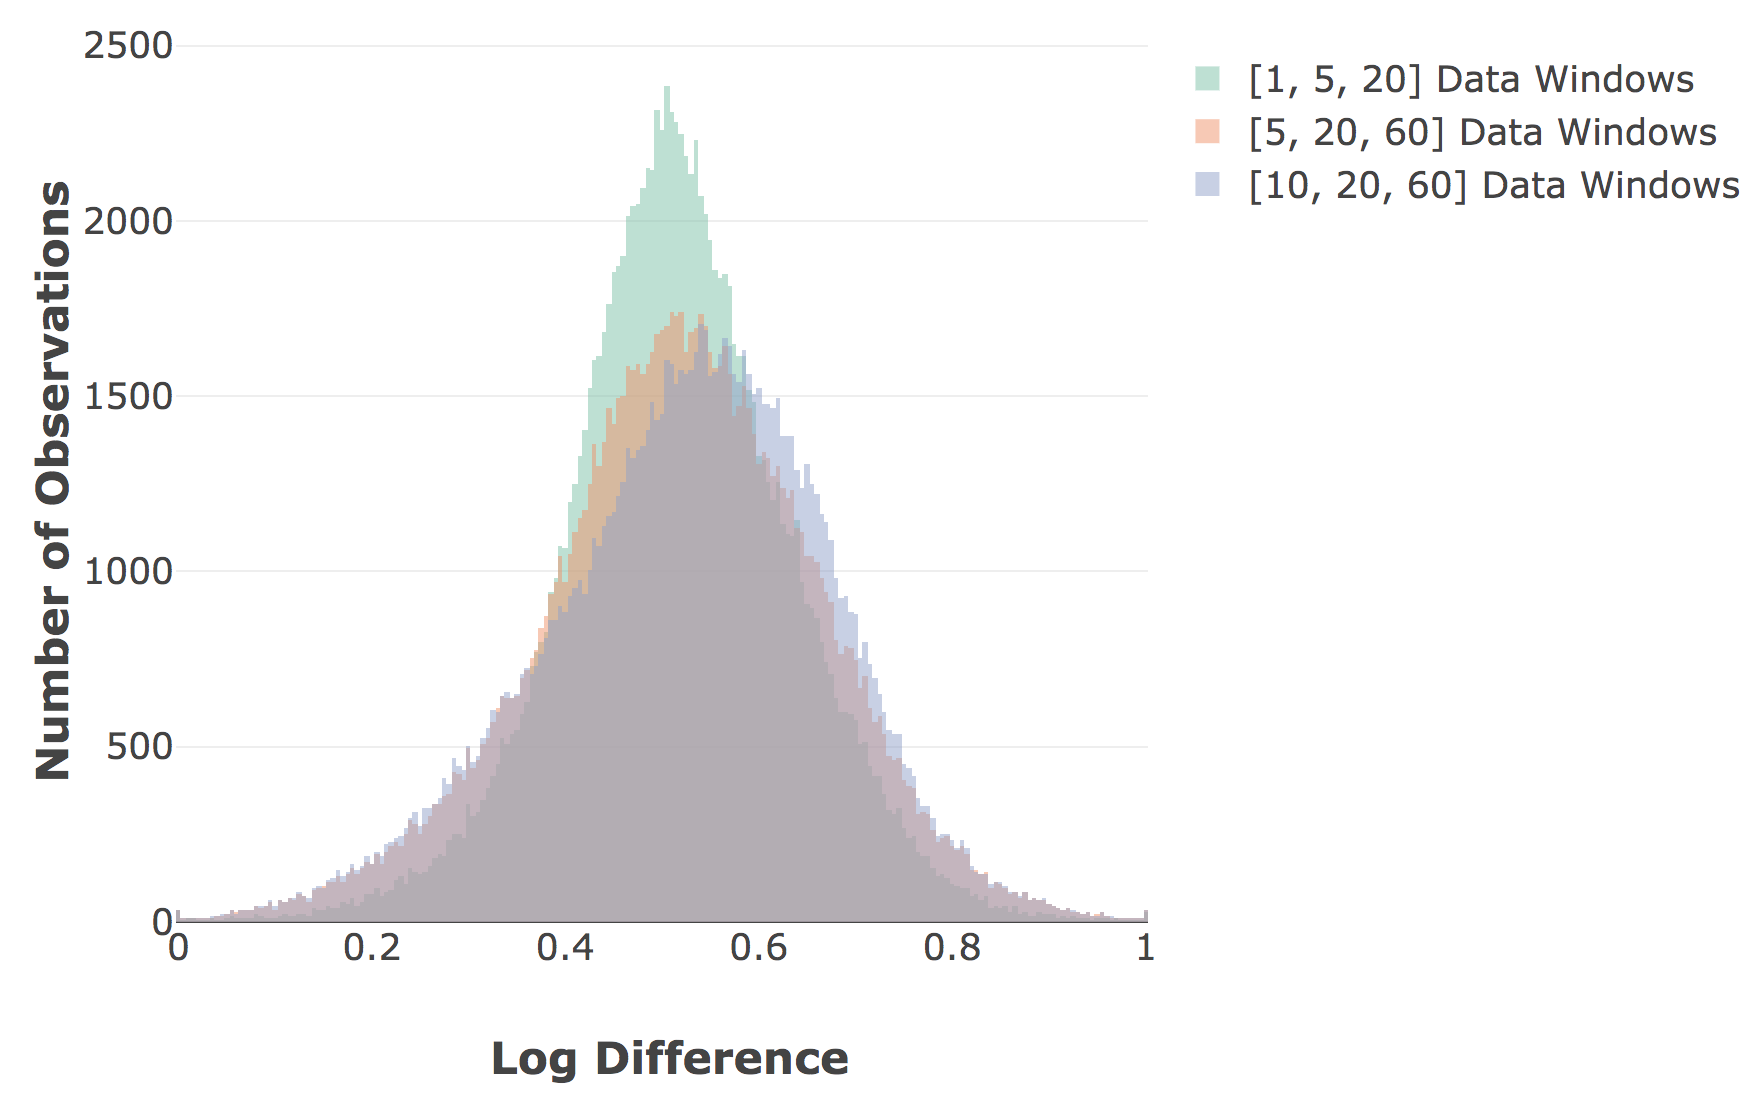
\includegraphics[scale=0.45]{images/results/8_2_determinants/actual_aggregate_dist.png}
			\caption{\textbf{Log Difference Distribution}
				\newline }
			\label{figure-actual_aggregate_dist}
		\end{subfigure}
		\begin{subfigure}{.99\textwidth}
			\centering 
			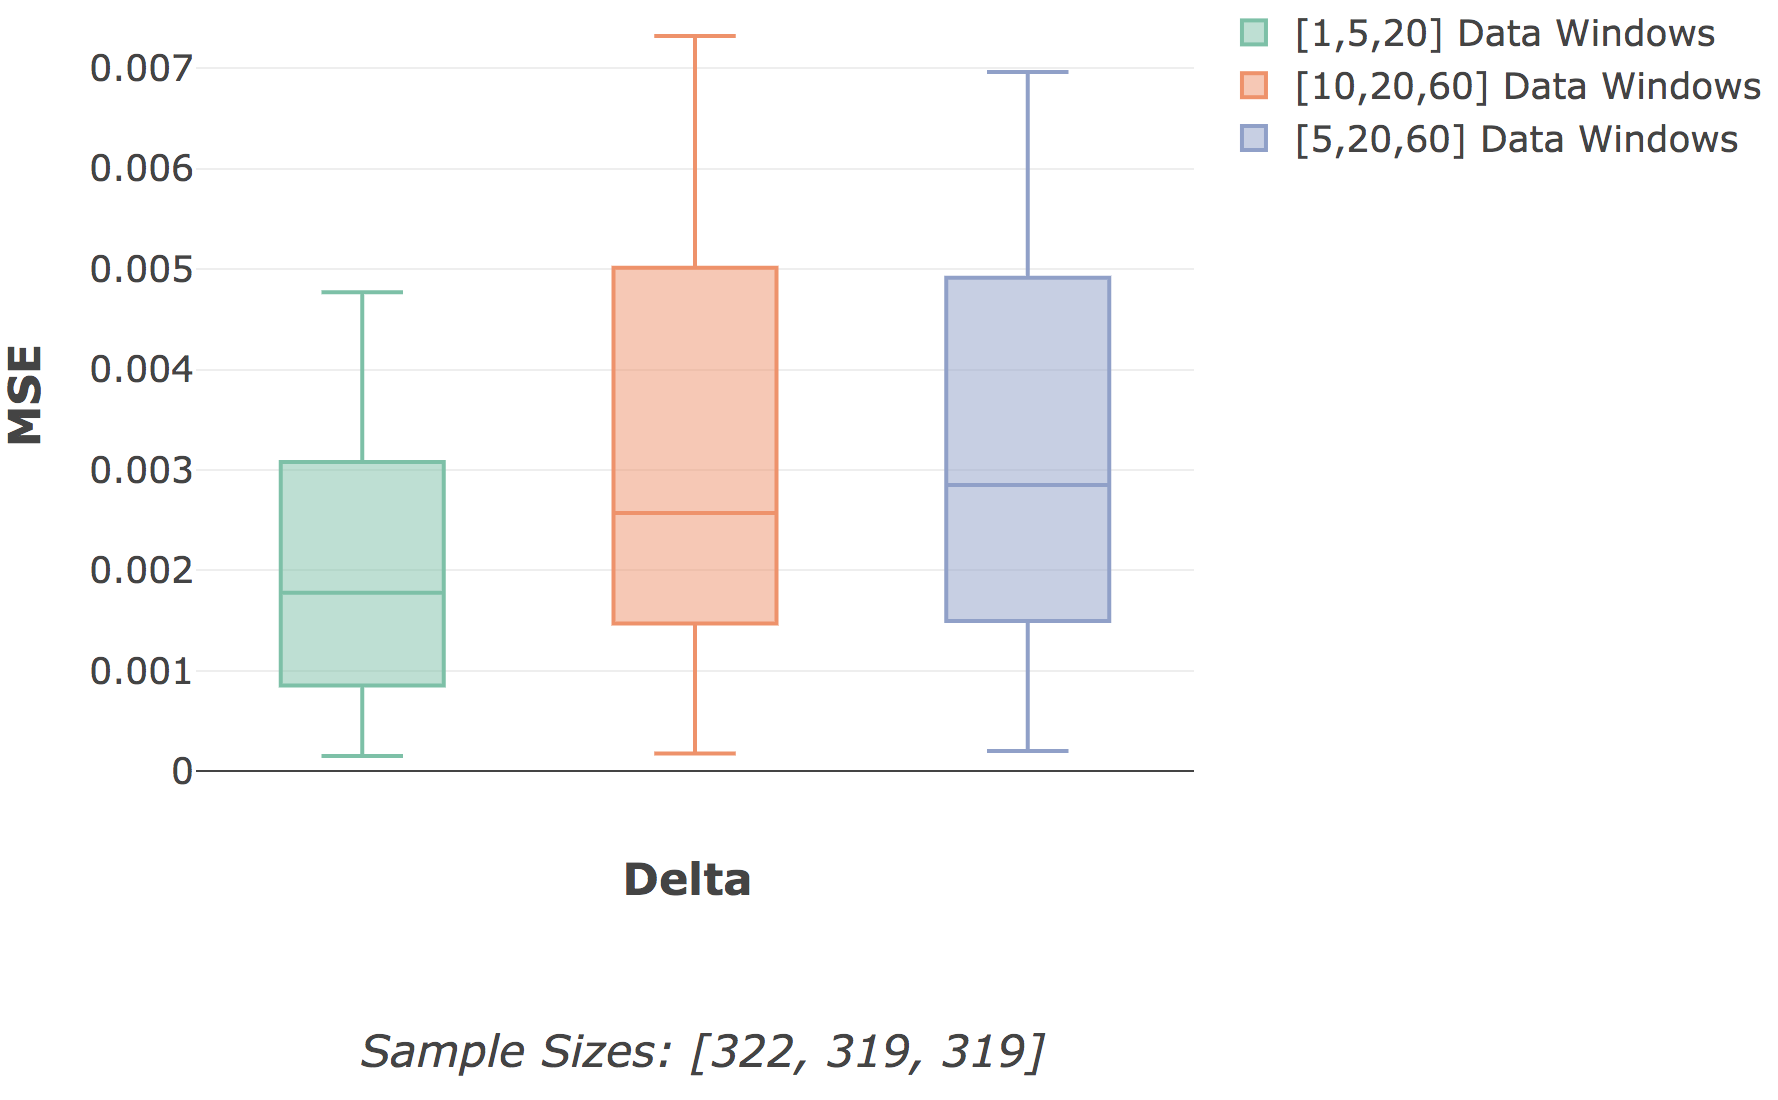
\includegraphics[scale=0.45]{images/results/8_2_determinants/actual_aggregation_mse.png}
			\caption{\textbf{SAE MSE Scores} 
				\newline }
			\label{figure-actual_aggregation_mse}
		\end{subfigure}
		\caption[SAE MSE Scores by Data Aggregations]
		{Dataset: Actual10 dataset (\ref{dataset_actual10}), Configuration 12 (\ref{config12})
			\newline  Figure (a) shows the distribution of values to be replicated by the SAE for actual data. Variances are quite different across the configurations ($\sigma_{[1,5,20]} = 0.118$, $\sigma_{[5,20,60]} = 0.146$, $\sigma_{[10,20,60]} = 0.150$). Smaller data windows are less likely to capture larger fundamental price changes, thus leading to these lower variances. This in turn, makes for easier replication for the SAE networks due to less variety in the sample set, which is seen in Figure (b) with the noticeably better performance in the [1, 5, 20] configuration.}
		\label{fig_data_sae_actual}
	\end{figure}
	
	
	
		\begin{figure}[H]
		\centering 
		\textbf{OOS P\&L by Data Aggregations}
		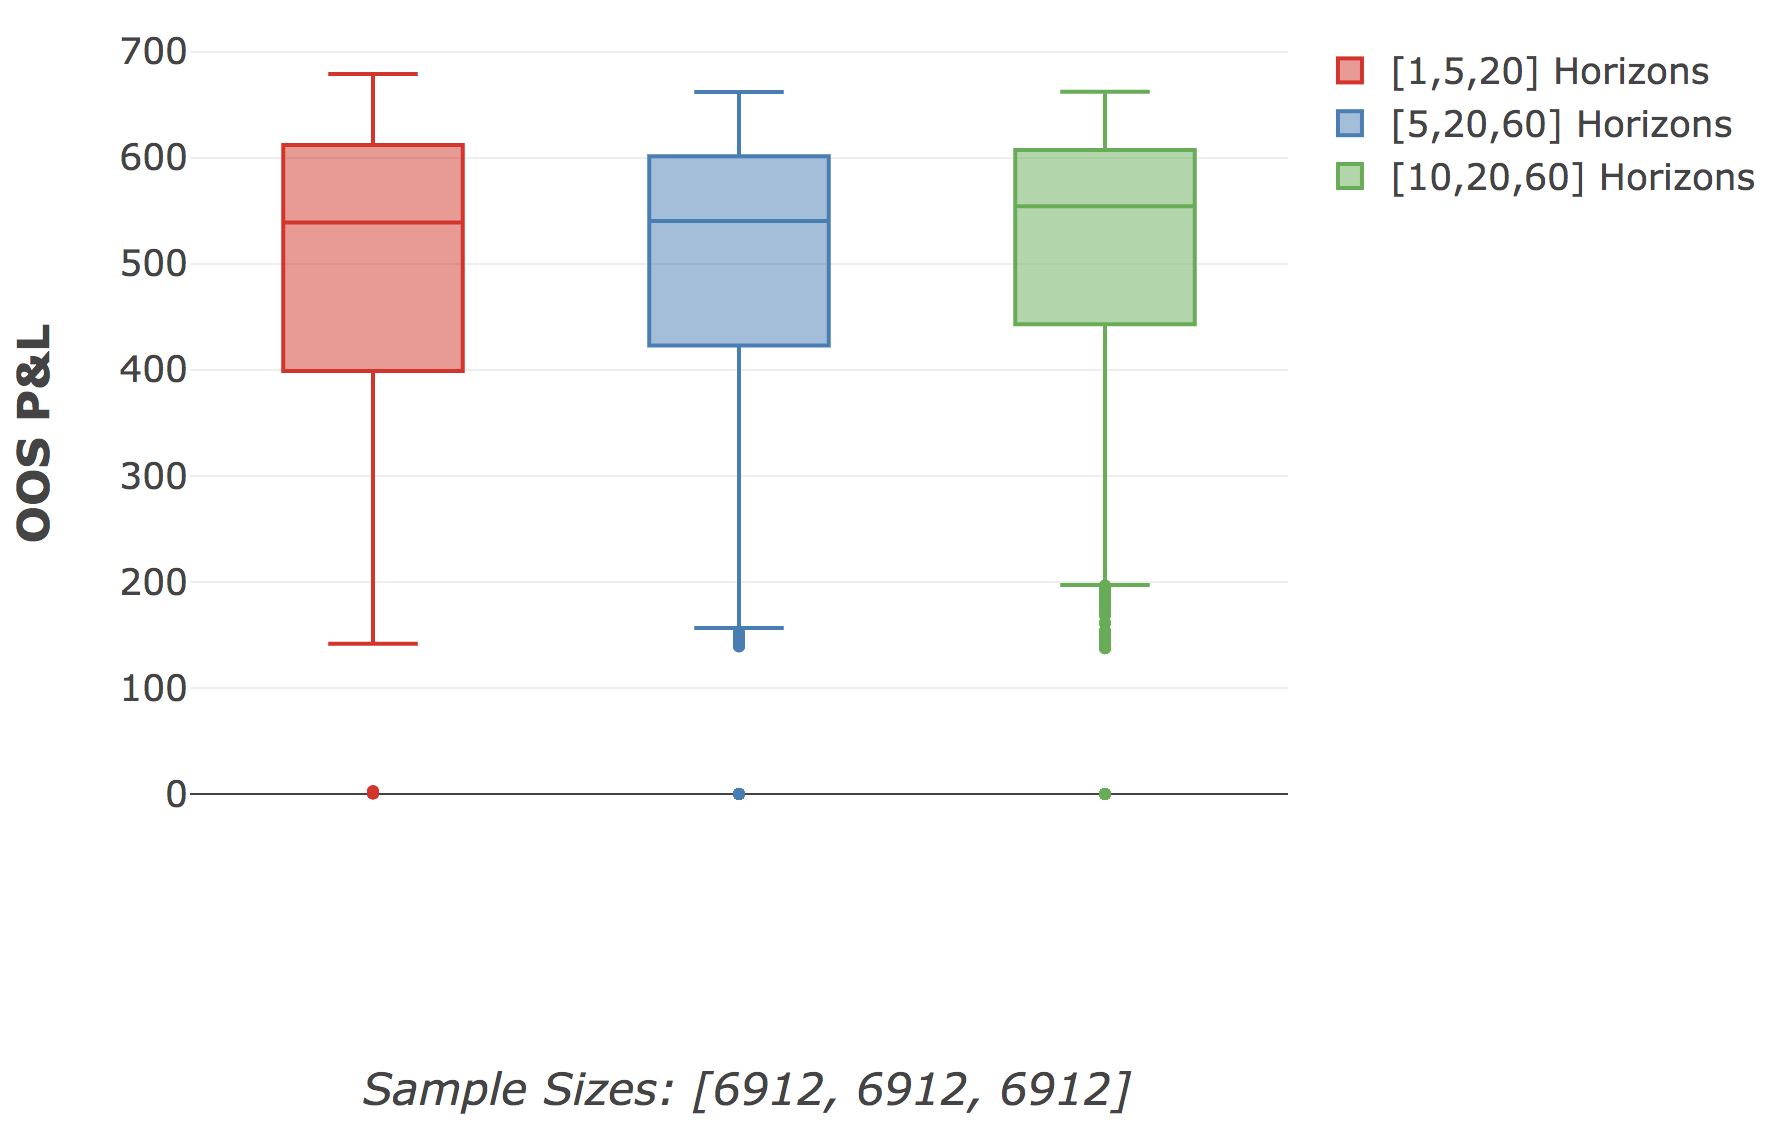
\includegraphics[scale=0.45]{images/results/8_2_determinants/actual_aggregation_pl.png}
		\caption[OOS P\&L by Data Aggregations]
		{
			Dataset: Actual10 dataset (\ref{dataset_actual10}), Configuration 13 (\ref{config13})
			\newline The OOS P\&L by data horizons shows the increased variance for shorter horizons, which is reduced as the horizons increase. The [1, 5, 20] configuration has a maximum which is 1.4\% higher than the longer configurations. With lower medians and minimums though, it is not clear that the maximum is indicative of anything beyond variance. This is the first view which suggests the higher risk and rewards dynamic with short term predictive strategies, and more reliable returns with longer term strategies. However, it is necessary to consider the other determinants to see this more clearly, as is continued below.}
		\label{figure-actual_aggregation_pl}
	\end{figure}
	
	\subsubsection{OGD Learning Rate}
	
	We found the OGD learning rate has the most distinctive impact on P\&L performance, as seen below in Figure \ref{figure-actual_ogd_lr}. The large differences between rates further highlights the unstable nature of financial systems. If dynamics were consistent across time, we would not expect to see such large changes in OOS performance due to larger learning rates. That we do, shows how the network's ability to adapt to more recent information is critical in determining performance. \newline
	
	The effect of the OGD learning rate on networks can once again be separated by the prediction strategy, with lower and higher learning rates performing better for different strategies. The learning rates and data aggregations can be seen below in Figure \ref{figure-actual_ogd_lr_data}.\newline
	
	\begin{figure}[H]
		\textbf{OOS P\&L by OGD Learning Rates}
		\centering
		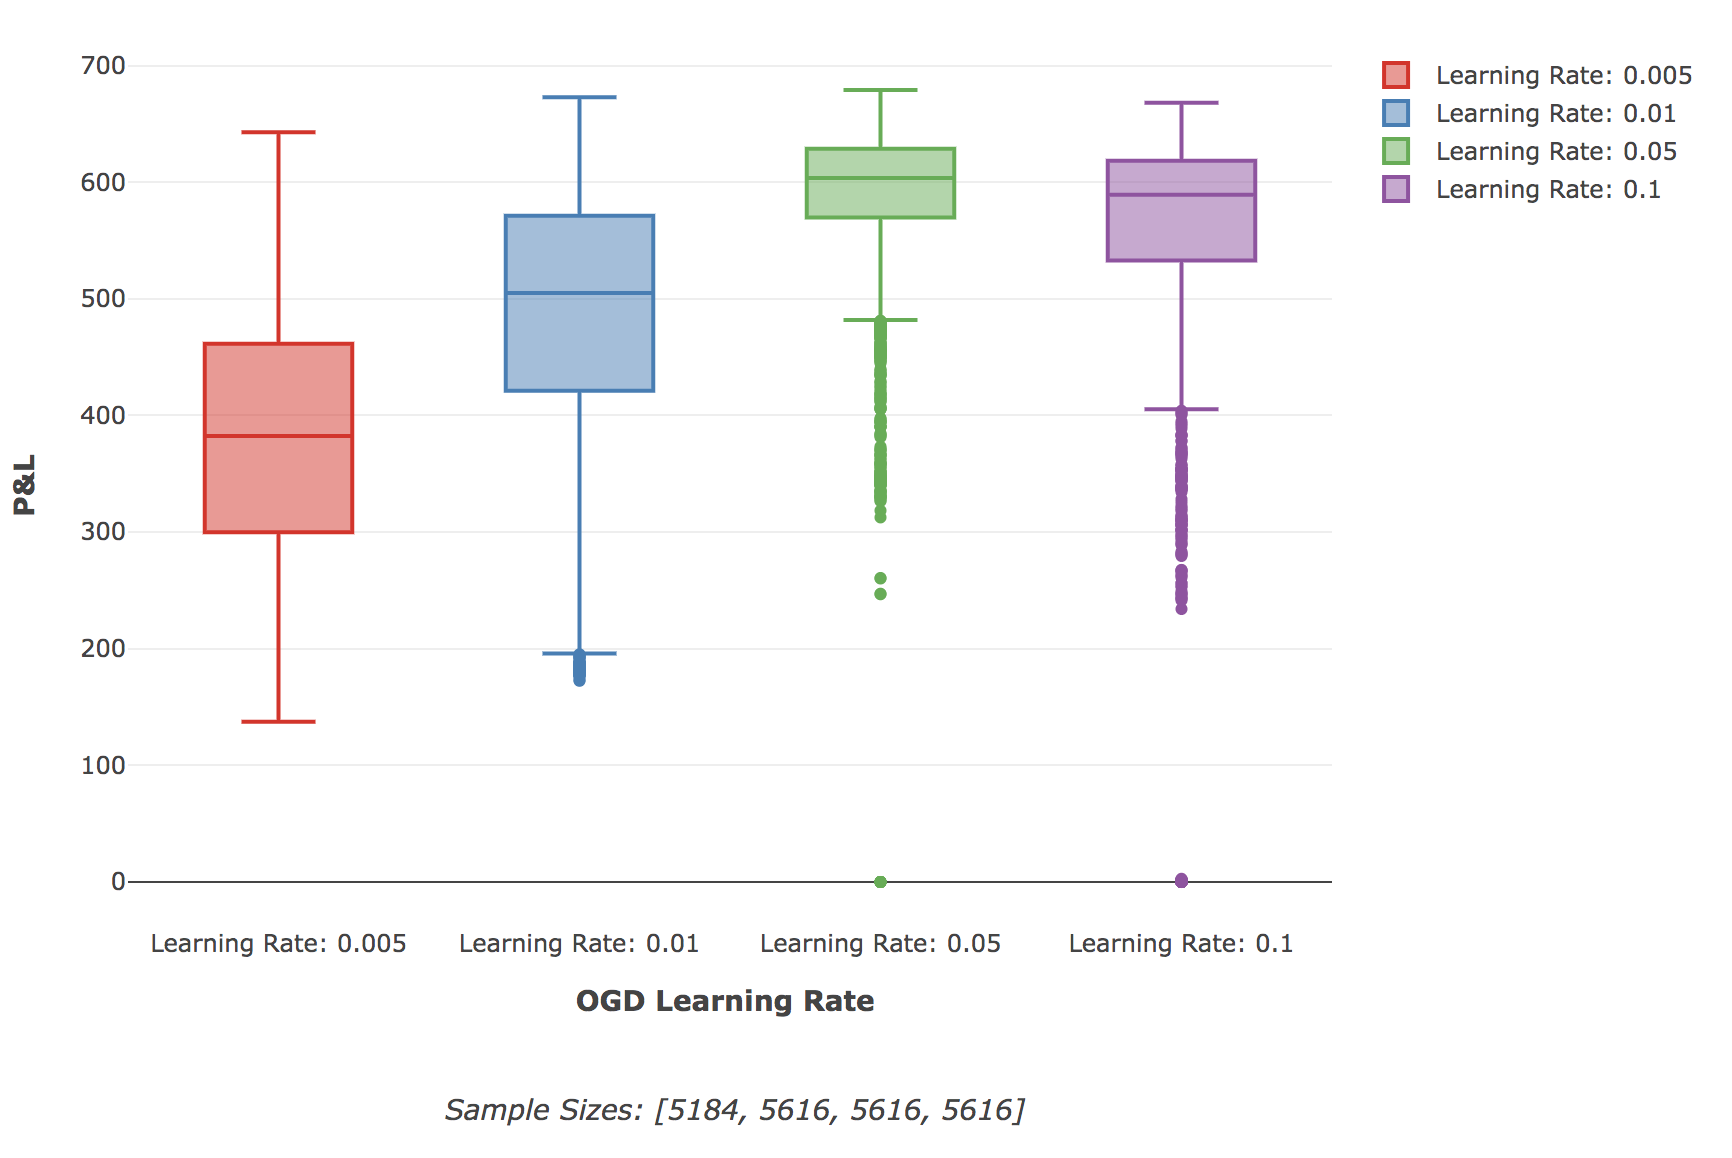
\includegraphics[scale=0.4]{images/results/8_2_determinants/actual_ogd_lr.png}
		\caption[OOS P\&L by OGD Learning Rates]
		{Dataset: Actual10 dataset (\ref{dataset_actual10}), Configuration 13 (\ref{config13})
			\newline The OOS P\&L performance for OGD learning rates is expectedly non-linear. Performance increased significantly from 0.001 to 0.05, and degraded thereafter as the network over corrected to noise and short term changes in the market. The higher learning rates, with networks more able to adapt to changing signal dynamics, also resulted in significantly lower variance in the P\&L delivered. }
		\label{figure-actual_ogd_lr}
	\end{figure}

	\begin{figure}[H]
		\textbf{OOS P\&L by OGD Learning Rates and Data Aggregations}
		\centering
		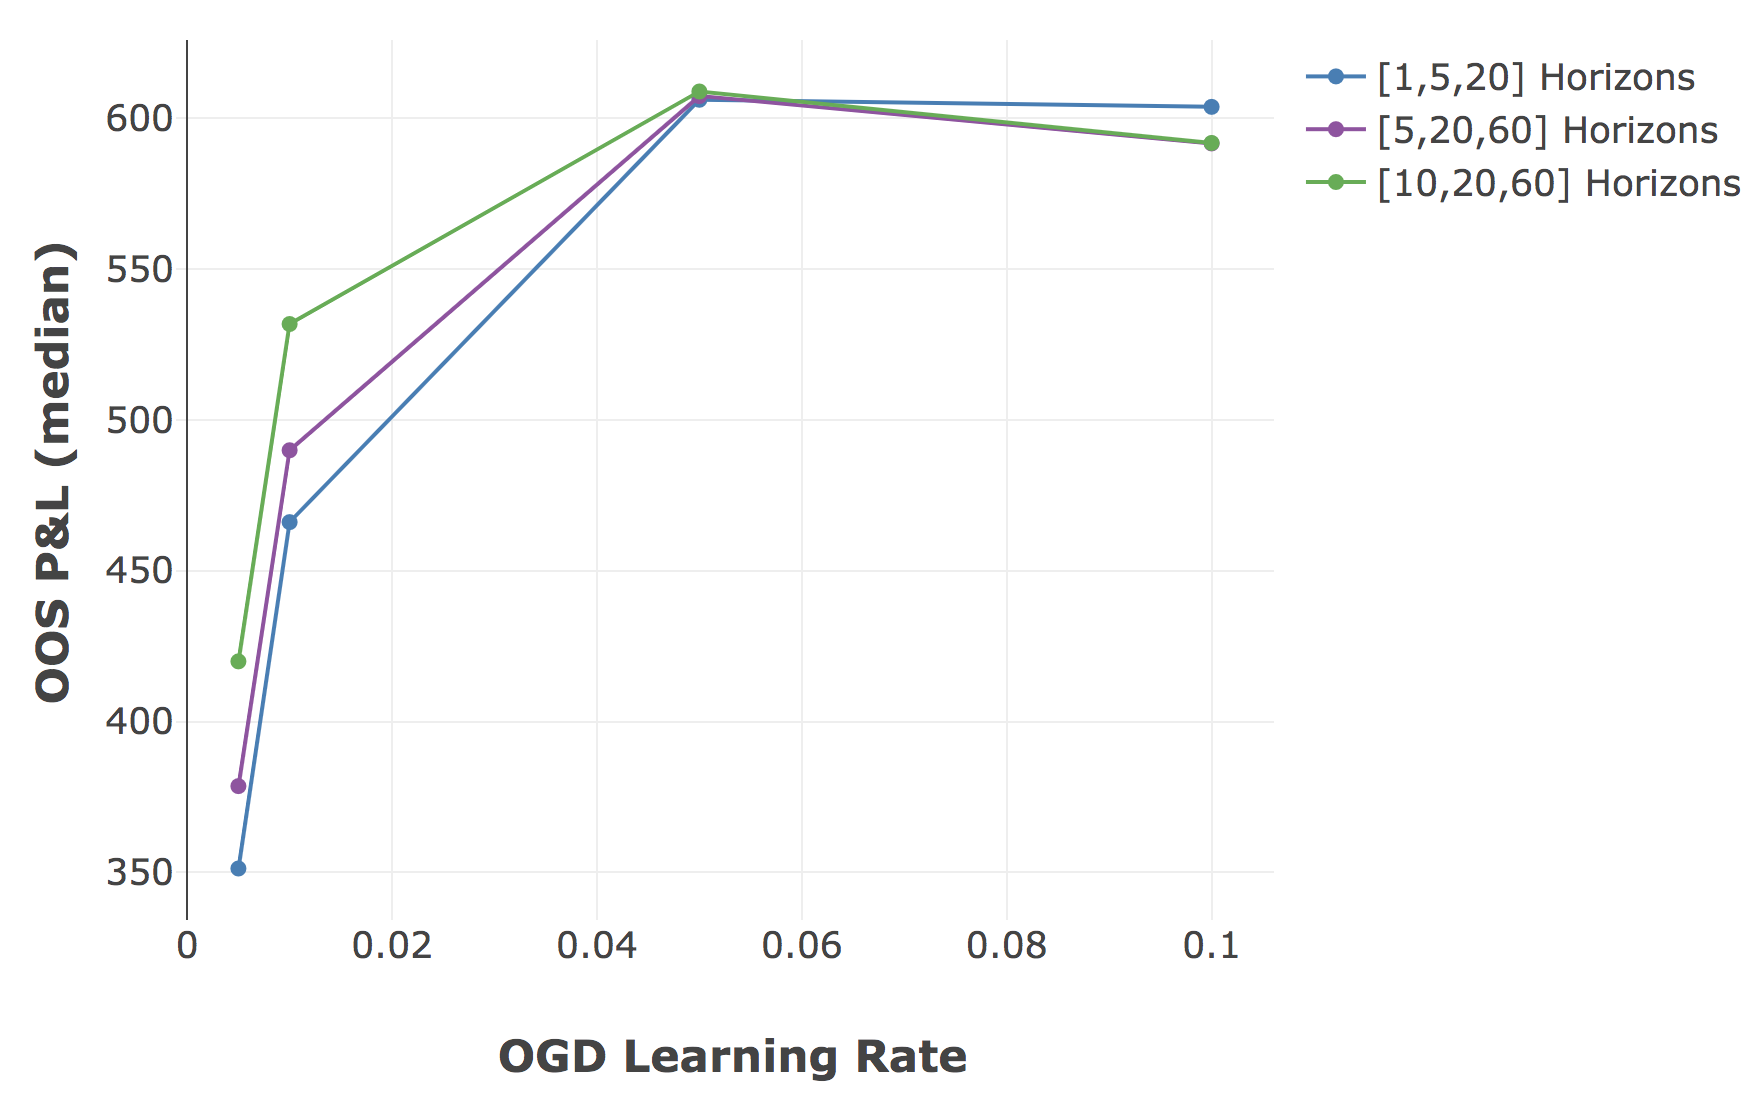
\includegraphics[scale=0.4]{images/results/8_2_determinants/OOS_OGDLR_Delta_PL_median.png}
		\caption[OOS P\&L by OGD Learning Rates and Data Aggregations]
		{Dataset: Actual10 dataset (\ref{dataset_actual10}), Configuration 13 (\ref{config13})
			\newline The median OOS P\&L by learning rate and data aggregation provides a view of the different prediction strategies. At lower learning rates, networks using long term changes and trends performed better as they benefit from smaller adjustments from one observation to the next. At high learning rates, networks using short term fluctuations performed better as they were able to more quickly adapt to changing dynamics and signals.}
		\label{figure-actual_ogd_lr_data}
	\end{figure}
	
	\subsubsection{Feature Selection}
	
	We found that feature selection through SAE dimensional reduction proves to be both possible and effective, though with complex behaviours and analyses. An important aspect to note is that the SAE networks were only trained on the first portion of IS data, and not updated afterwards. In light of changing dynamics in financial markets then, an effective SAE feature reduction in this process is an optimization that may be limited to a certain time period. However, this optimisation may not generalise well in a different context (i.e. OOS). \newline
	
	Inspection of the nature of features learnt is difficult, though results show that the features can be categorised into 2 groups: larger encodings (25, 20, 15) which performed the equivalent of denoising or smoothing, and smaller encodings (10, 5) which performed more robust feature selection of legitimate properties\footnote{Input data was 10 assets with 3 horizon aggregations each, resulting in an input size of 30 at each timestep.}.\newline

	While the OOS performance of the larger encoding sizes mostly behaved as expected, the SAEs with encoding sizes of 5 and 10 were more inconsistent. In line with the view of changing dynamics within financial markets over time, we saw that SAEs with encoding of 10 overfit to particular features. These performed well for strategies focusing on long term trends, but were pathological for the strategies focusing on short term fluctuations. The SAEs with encoding size of 5 had more dependable performance, possibly because the small encoding layer acts as a form of regularization. The regularization would force the SAE to learn more consistently generalisable features. These dynamics are explored more in Figures \ref{figure-encoding_pl_median} and \ref{figure_ogdlr_delta_encoding_groups} below.  \newline
	
	The most noteworthy results we saw were SAE networks with encoding size of 5, which learnt generalisable features for 10 assets with 3 data aggregations each. Their performances were often on par or better than the higher encoding sizes, or no encoding at all, as seen in Figure \ref{figure_OOS_Encoding_PL_Box} below. One of the 2 primary goals of this paper was to determine if feature reduction is possible and benefical, which we are able to answer here. The performance of the 5-encoding networks, with an 83\% reduction in input data, is clear evidence of the efficacy and potential of feature selection in financial times series.  \newline
	
	\begin{figure}[H]
		\centering
		\textbf{IS Performance by Encoding Size}
		\begin{subfigure}{0.99\linewidth}
			\centering 
			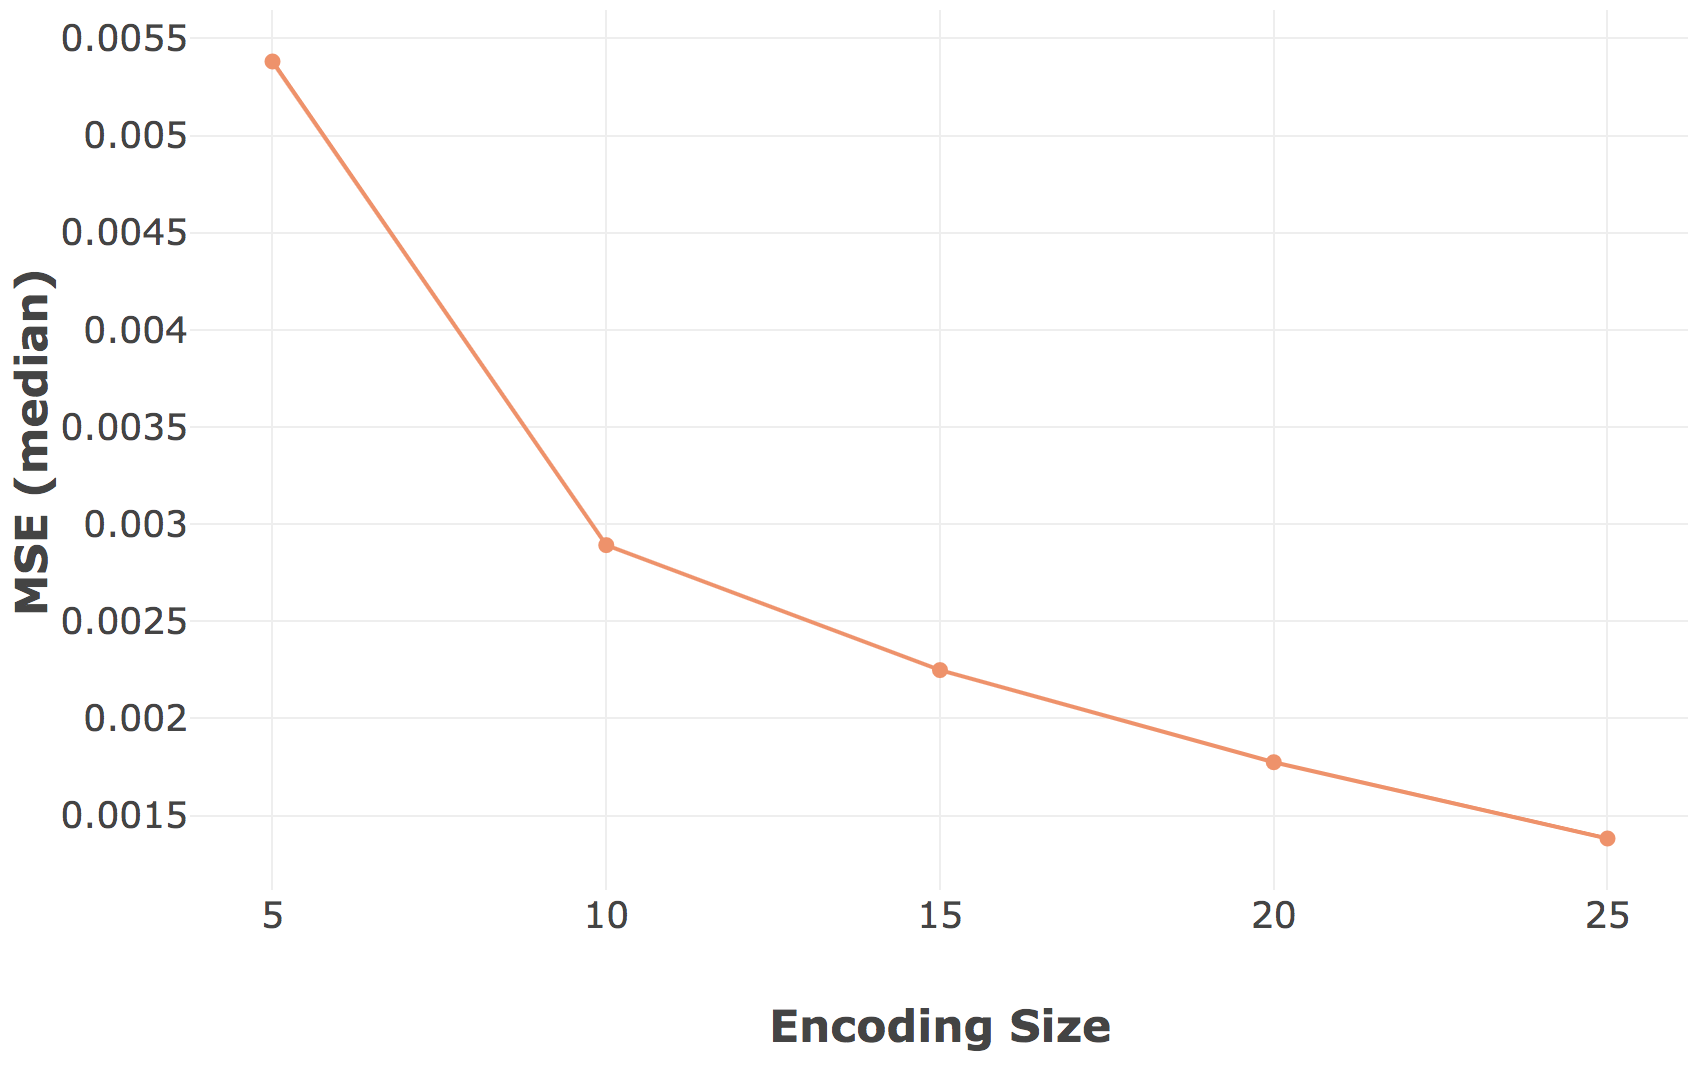
\includegraphics[scale=0.4]{images/results/8_2_determinants/actual_sae_mse.png}
			\caption[MSE By Feature Selection Size]{MSE By Feature Selection Size}
			\label{figure-actual_sae_mse}
		\end{subfigure}
		\begin{subfigure}{0.99\linewidth}
		\centering 
		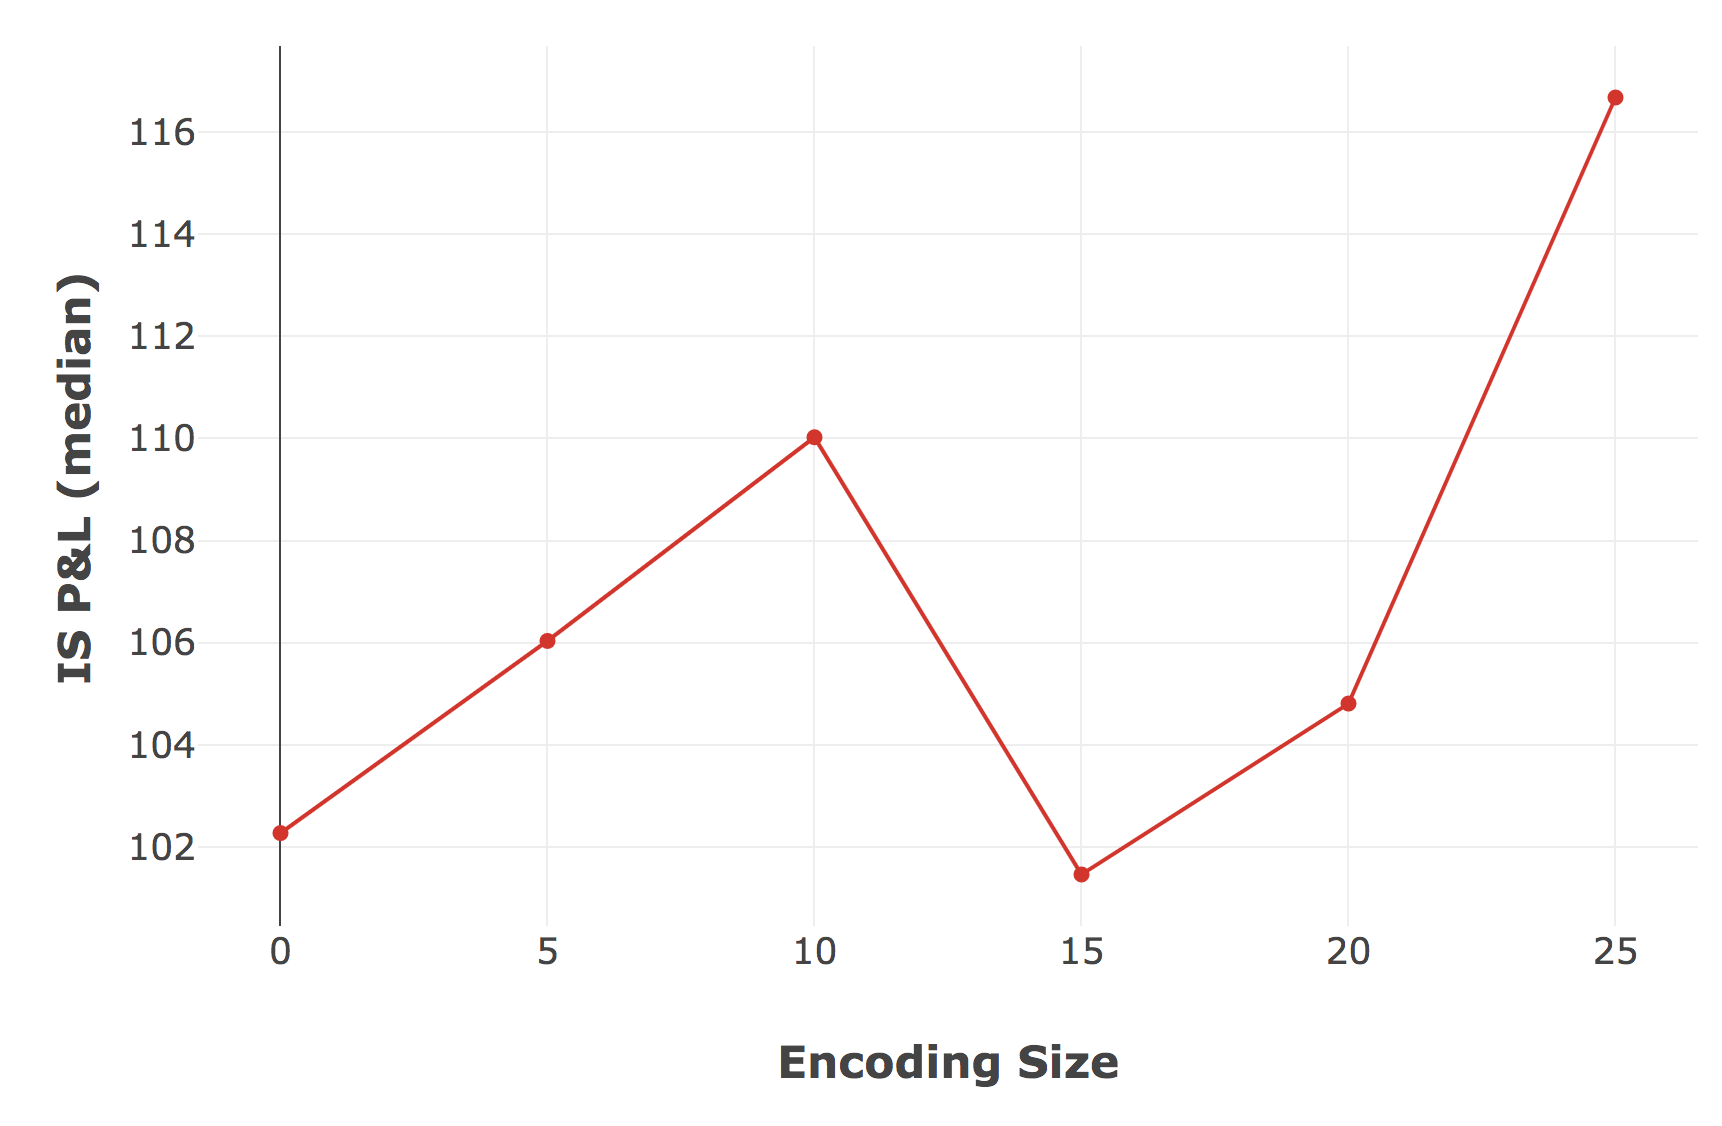
\includegraphics[scale=0.4]{images/results/8_2_determinants/IS_Encoding_PL_median.png} 
		\caption[IS SAE Performance: MSE and P\&L by Encoding Size]{IS P\&L by Encoding Size}
		\label{figure-IS Encoding_PL_median}
		\end{subfigure}
	\caption[IS Performance by Encoding Size]
	{Dataset: Actual10 dataset (\ref{dataset_actual10}), Configurations 11 and 12 (\ref{config11}, \ref{config12})
		\newline Figure (a) shows the MSE scores at different encoding sizes. While feature selection and reduction is possible through the SAE networks, the ability to reproduce input precisely does decrease monotonically with the encoding layer size. 
		\newline Figure (b) shows the IS P\&L for the same groups. This provides a different assessment, showing a clear increase in P\&L at the 5 and 10 encoding sizes (``0'' indicates no feature reduction was done). This is indicative of the 2 different types of features learnt: sizes 15, 20 and 25 were smoothing or denoising the data and so reproductive MSE was correlated to P\&L performance; conversely, at sizes 5 and 10 the SAE began learning more fundamental features of the data and so the relative reproductive MSE score is not a clear indicator for P\&L performance.}
	\end{figure}
	
	\begin{figure}[H]
		\centering 
		\textbf{OOS P\&L By Feature Selection Size and OGD Learning Rate}
		\begin{subfigure}{1.0\linewidth}
			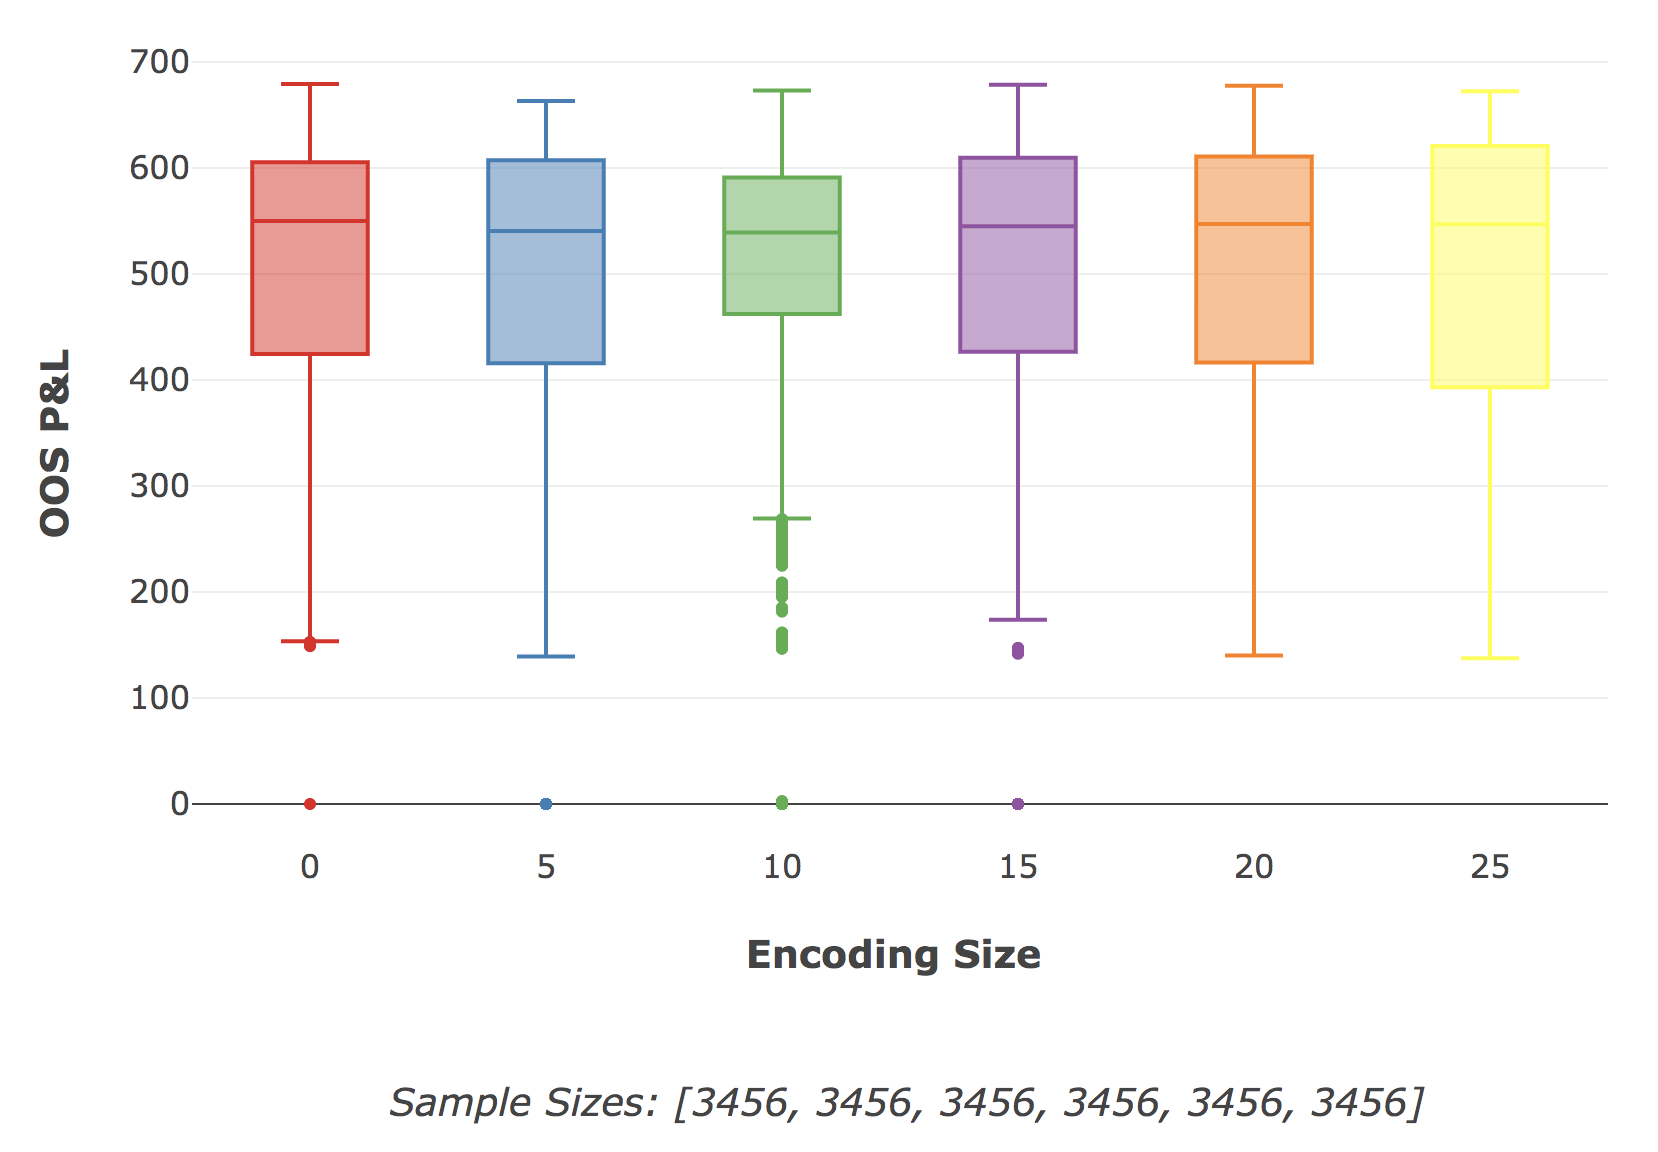
\includegraphics[scale=0.45]{images/results/8_2_determinants/OOS_Encoding_PL_Box.png} 
			\caption[OOS P\&L by Encoding Size]{OOS P\&L by Encoding Size}
			\label{figure_OOS_Encoding_PL_Box}
		\end{subfigure}	
		\begin{subfigure}{1.0\linewidth}
			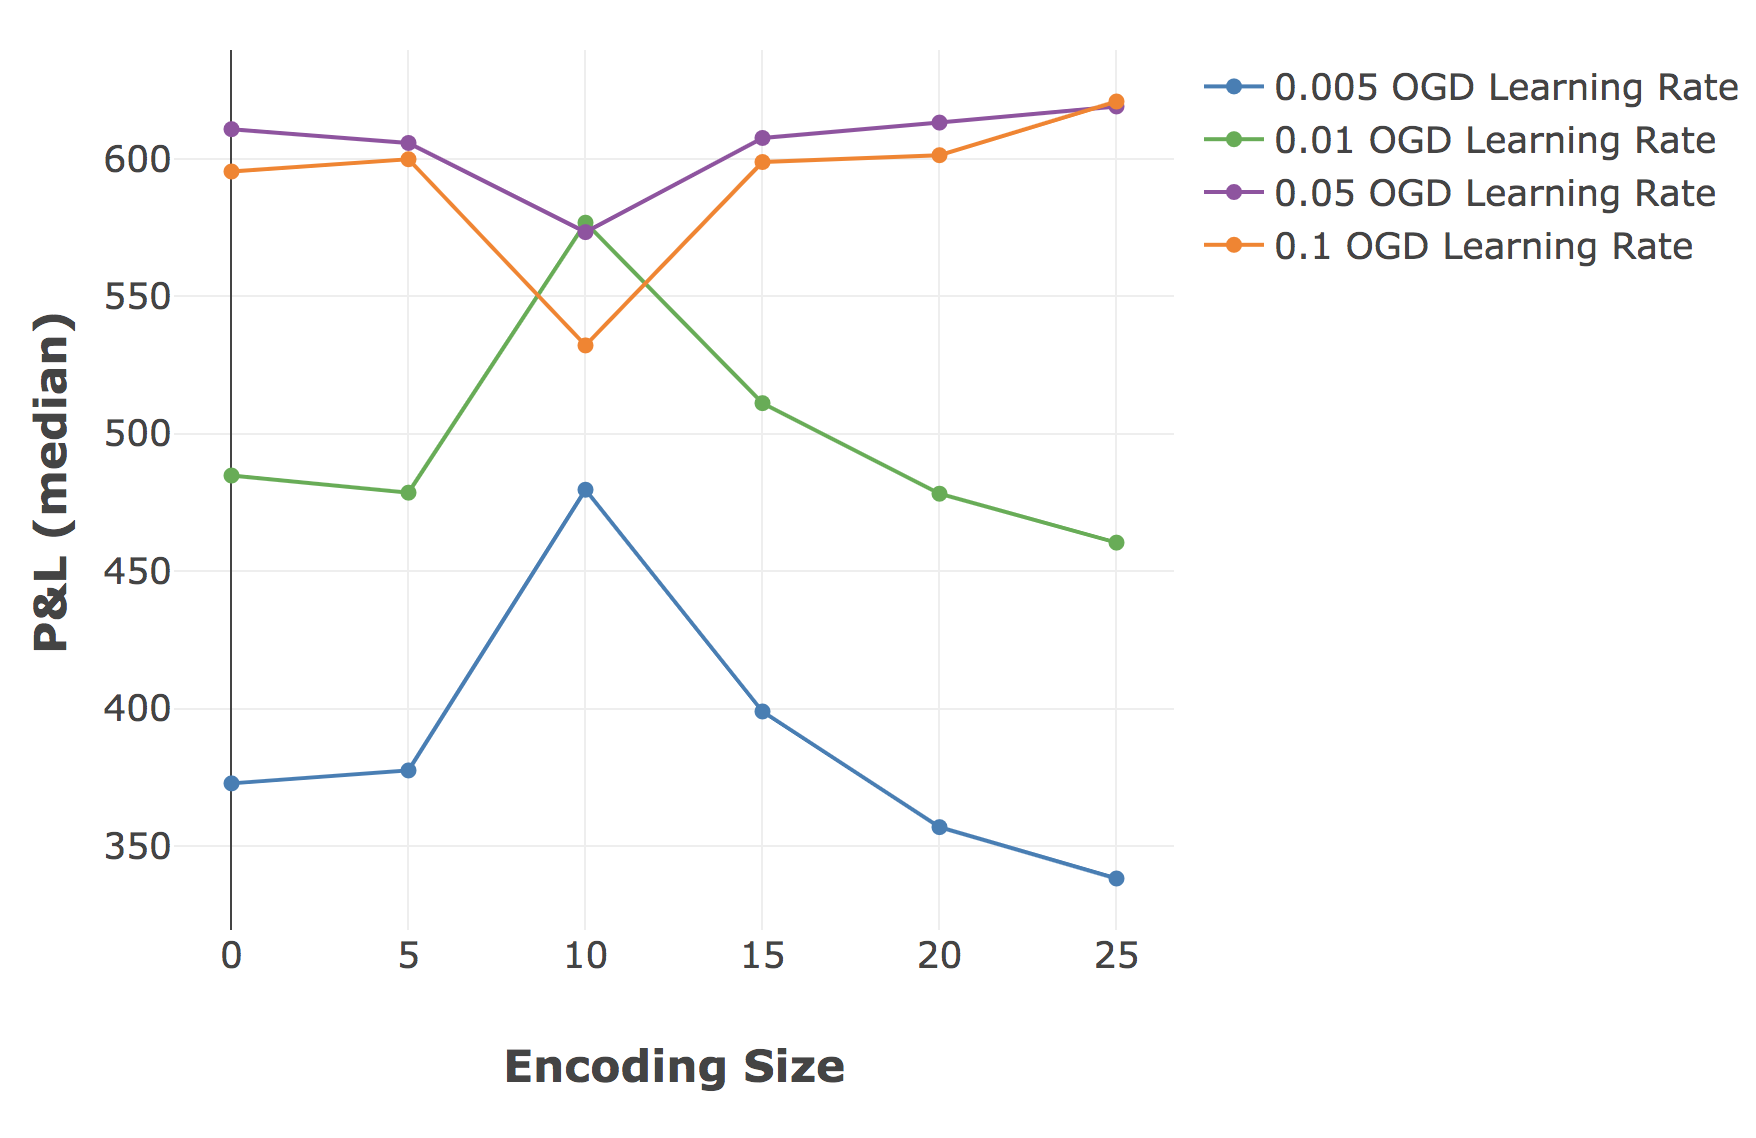
\includegraphics[scale=0.45]{images/results/8_2_determinants/encoding_pl_median.png} 
			\caption[OOS P\&L by Encoding Size and Learning Rate]{OOS P\&L by Encoding Size and Learning Rate}
		\end{subfigure}	
		\caption[OOS P\&L By Feature Selection Size and OGD Learning Rate]
		{Dataset: Actual10 dataset (\ref{dataset_actual10}), Configuration 11 (\ref{config11})		
		\newline Figure (a) shows the OOS P\&L performance for all encoding sizes, with an encoding of 0 indicating no feature reduction. It is interesting to note that at their best, almost all encodings were able to offer equitable performance. There was however a general variance reduction from 25 to 15, with 10 and 5 behaving somewhat differently. Figure (b) gives us far more insight into the dynamics causing the changing P\&L. The lower learning rates (0.005, 0.01) performed best with strategies using long term trend pricing (as seen in Figure \ref{figure-actual_ogd_lr_data}). The 10 feature encoding appeared to optimise specifically for this perspective. The optimisation caused outperformance at the lower learning rates and detrimental performance at higher learning rates (which perform best with short term fluctuation strategies). The 15 to 25 encodings showed a better association to the short term strategies, where higher encodings and higher learning rates offer the best performance. Notably, the 5 feature encoding offered the most consistent performance across learning rates, further emphasising the learning of generalisable features. These dynamics are explored further in Figure \ref{figure_ogdlr_delta_encoding_groups}.}
	\label{figure-encoding_pl_median}
	\end{figure}
		
		\newpage
		\begin{figure}[H]
			\centering
			\textbf{OOS P\&L By Feature Selection Size, OGD Learning Rate and Data Horizons}
			\begin{subfigure}{0.48\linewidth}
				\centering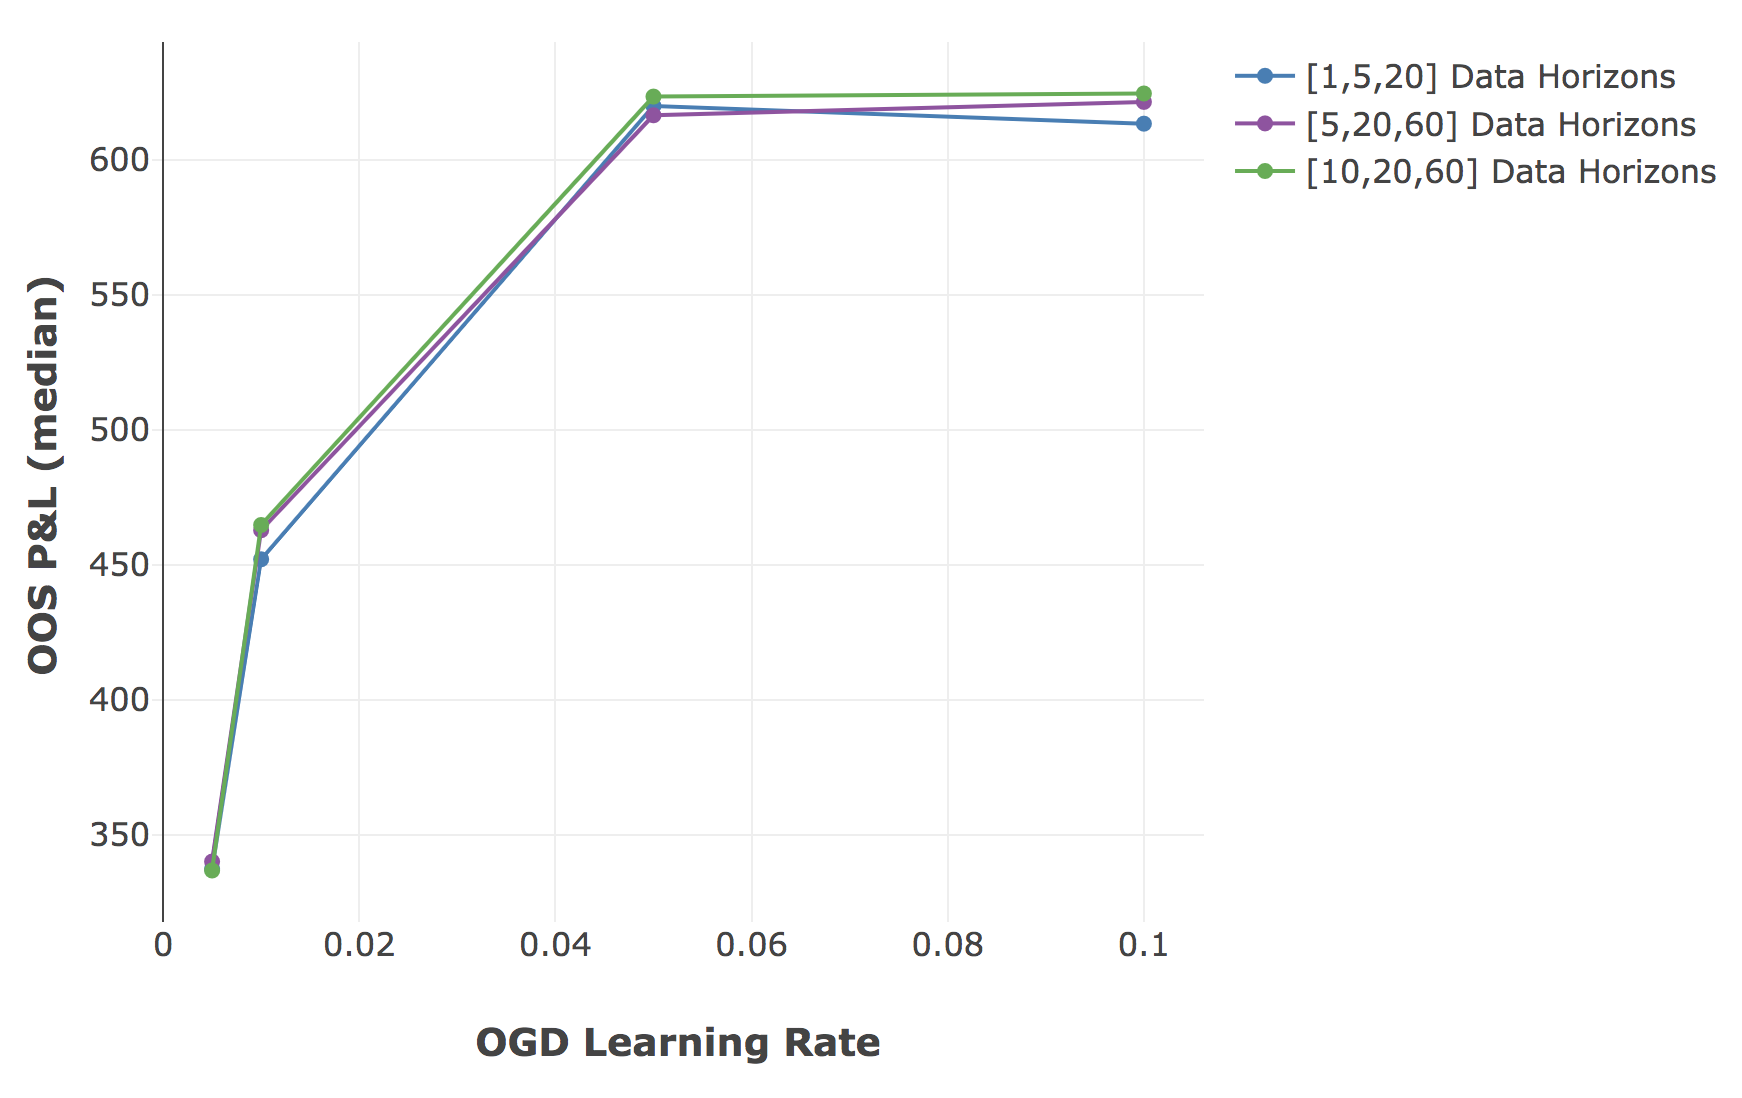
\includegraphics[scale=0.33]{images/results/8_2_determinants/OOS_OGDLR_Delta_Encoding_25_median.png}
				\caption{Encoding Size of 25}
			\end{subfigure}
			\begin{subfigure}{0.49\linewidth}
				\centering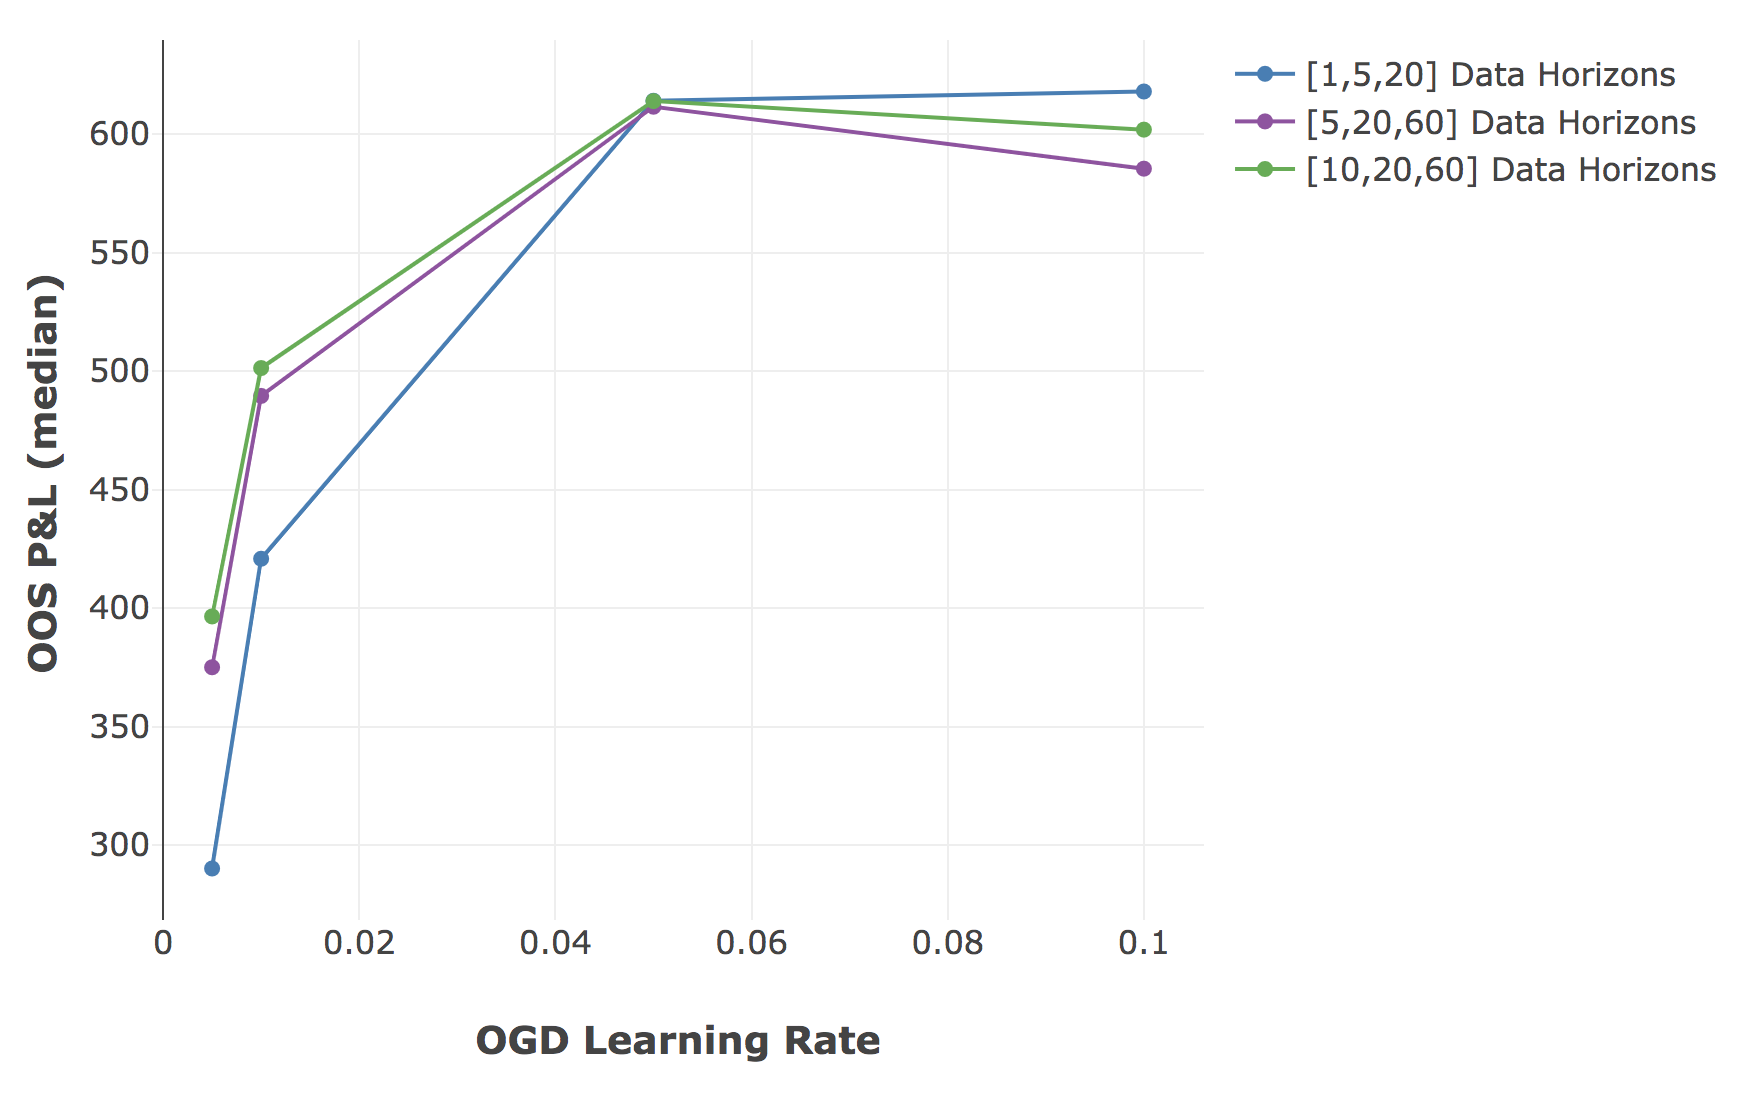
\includegraphics[scale=0.33]{images/results/8_2_determinants/OOS_OGDLR_Delta_Encoding_20_median.png}
				\caption{Encoding size of 20}
			\end{subfigure}%\vspace{10pt}
			
			\begin{subfigure}{0.48\linewidth}
				\centering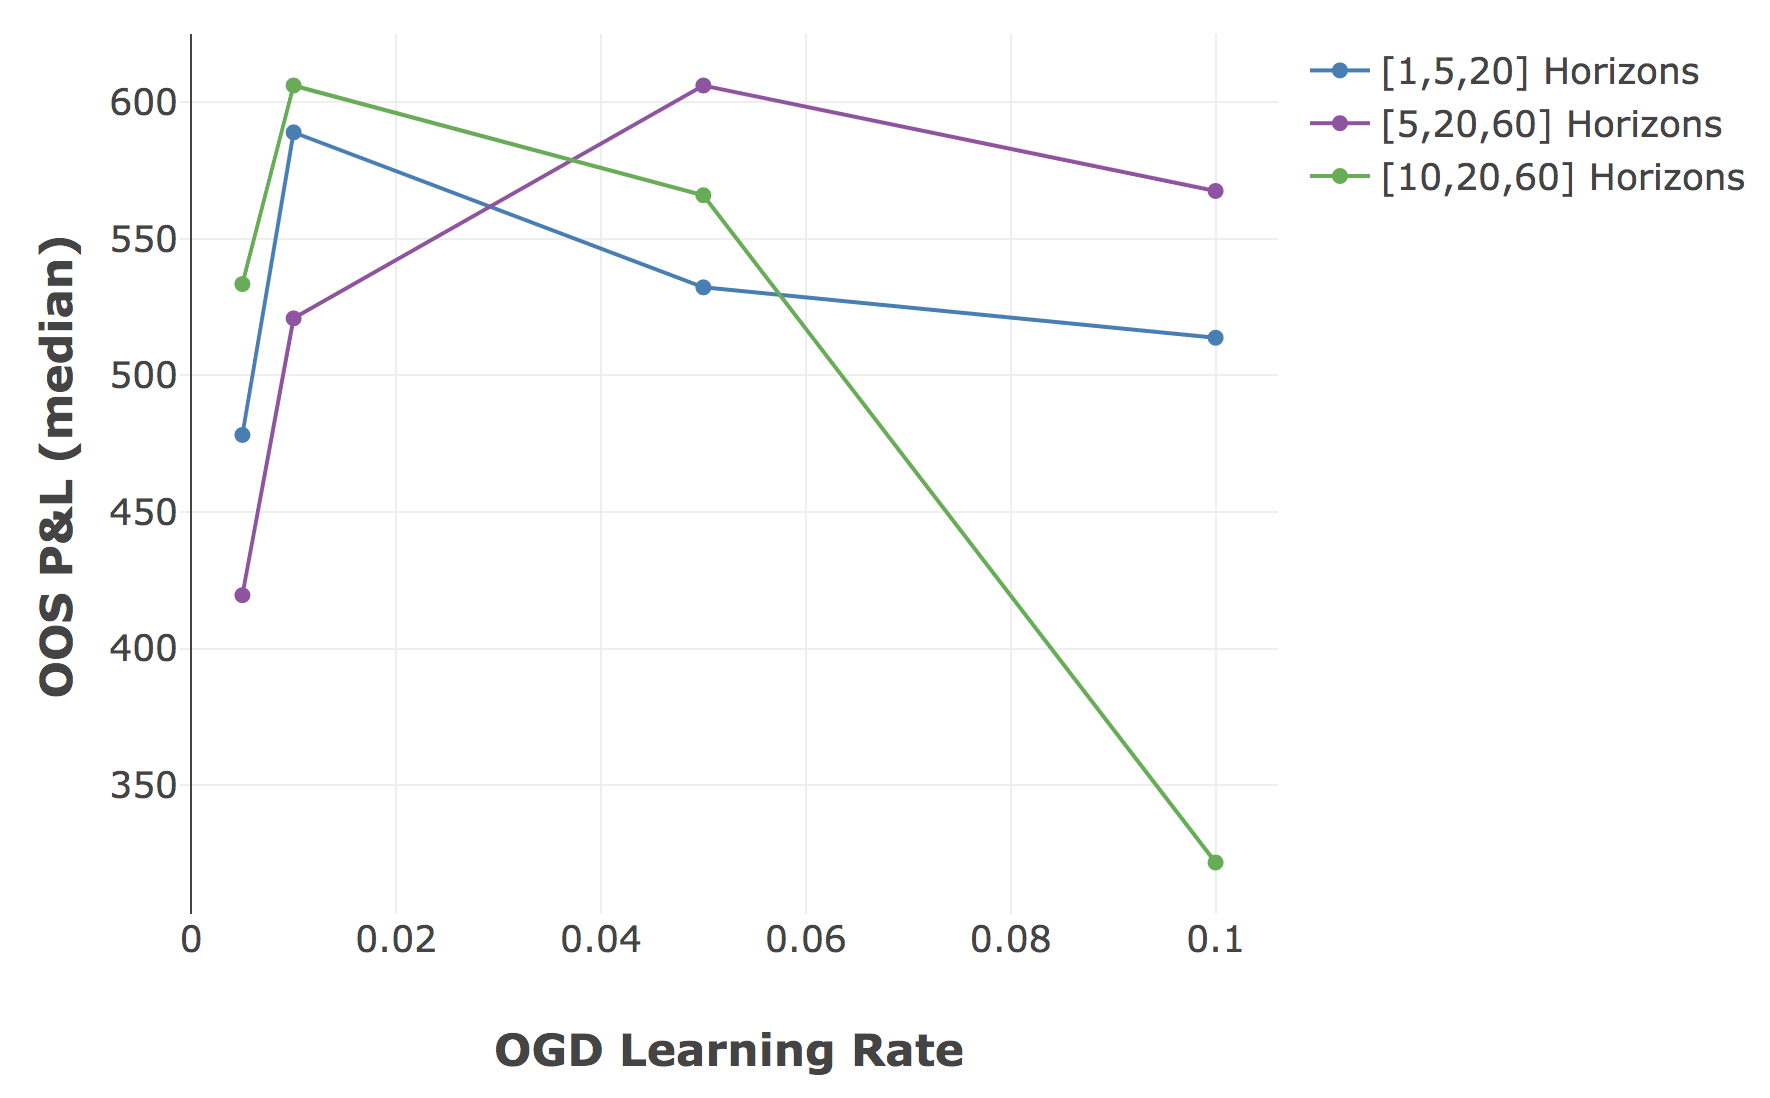
\includegraphics[scale=0.33]{images/results/8_2_determinants/OOS_OGDLR_Delta_Encoding_10_median.png}
				\caption{Encoding Size of 10}
			\end{subfigure}%
			\begin{subfigure}{0.49\linewidth}
				\centering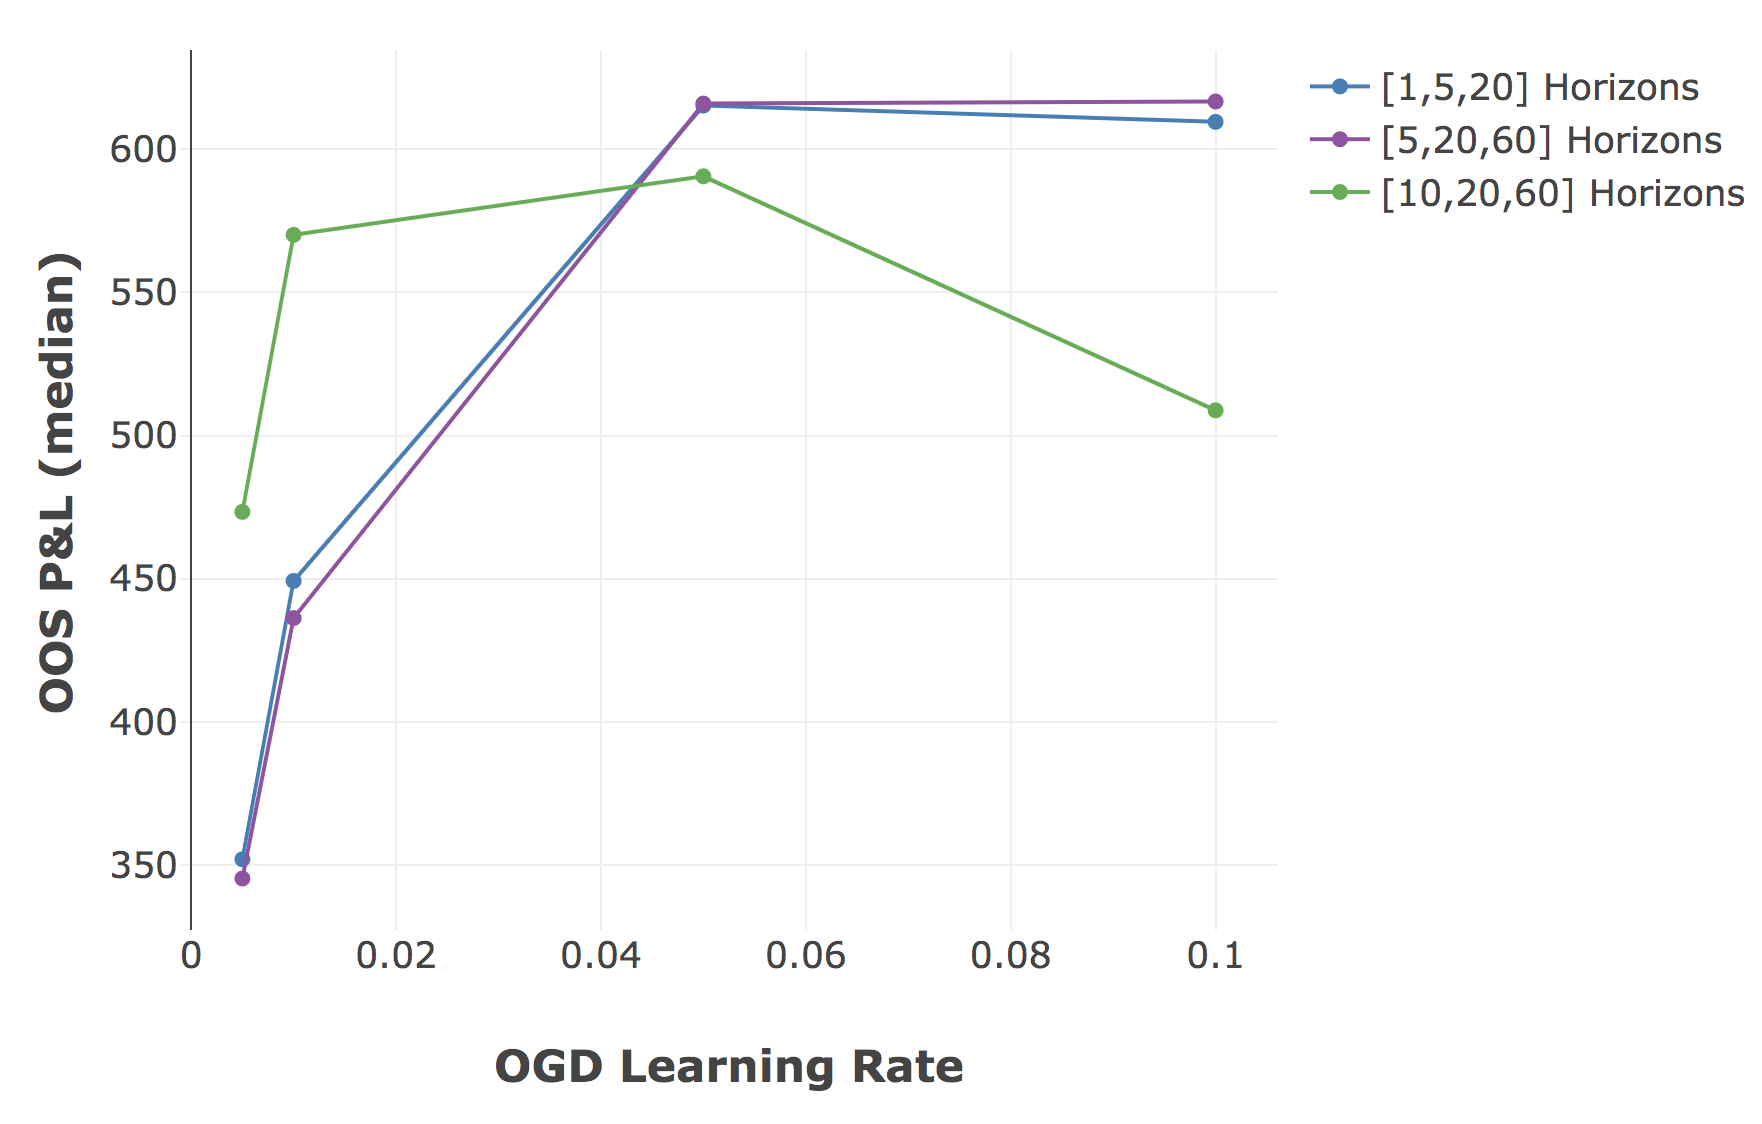
\includegraphics[scale=0.33]{images/results/8_2_determinants/OOS_OGDLR_Delta_Encoding_5_median.png}
				\caption{Encoding Size of 5}
			\end{subfigure}
		\caption[OOS P\&L By Feature Selection Size, OGD Learning Rate and Data Horizons]
		{Dataset: Actual10 dataset (\ref{dataset_actual10}), Configuration 11 (\ref{config11})		
			\newline The 4 plots above offer a cohesive view of all 3 primary determinants of OOS P\&L. At encoding sizes of 25 and 20, which were largely smoothing the input, the feature reduction had less material impact and so the relation between data horizons and learning rates is more prominent. Longer horizons deliver higher P\&L with lower learning rates (and so smaller adjustments), while short term horizons outperform with large learning rates (and so an ability to adapt quickly). The SAEs with encoding size 10 showed the most inconsistent behaviour, clearly having overfit to the long term features. This resulted in high performance with the low learning rates and longer horizons, and extremely poor performance with higher learning rates and longer horizons. The encoding size 5 learnt a more robust feature selection, resulting in the best of longer horizons at low learning rates, and the best of shorter horizons at larger learning rates. }
			\label{figure_ogdlr_delta_encoding_groups}
		\end{figure}
		
		
		
		
		\newpage

	\subsection{Value of Historical Signal}\label{results_data_hist}
		
	We ran experimental trials to test the hypothesis that the amount of historical IS data available is of limited use, and that the real value is in broader current and cross sectional data. This idea is in line with the understanding that financial markets are inherently complex, adaptive and dynamic, as discussed more broadly in Section \ref{lr_TechnicalAnalysis}. With this in mind, and especially so in light of a fundamentally changing macroeconomic landscape, there is limited reason to believe that the functions and relations that may have governed the asset prices 10-15 years ago would still be dominant today. We found the P\&L results validate this idea, as seen in Figures \ref{figure-results_pl_max_epochs} and \ref{figure-results_it3_validationset}. We saw that extensive training on past data may be akin to pre-training network weights at best, and counterproductive in overfitting to dynamics that no longer exist at worst.
	
	\begin{figure}[H]
		\centering 
		\textbf{OOS P\&L by IS Training Epochs}
		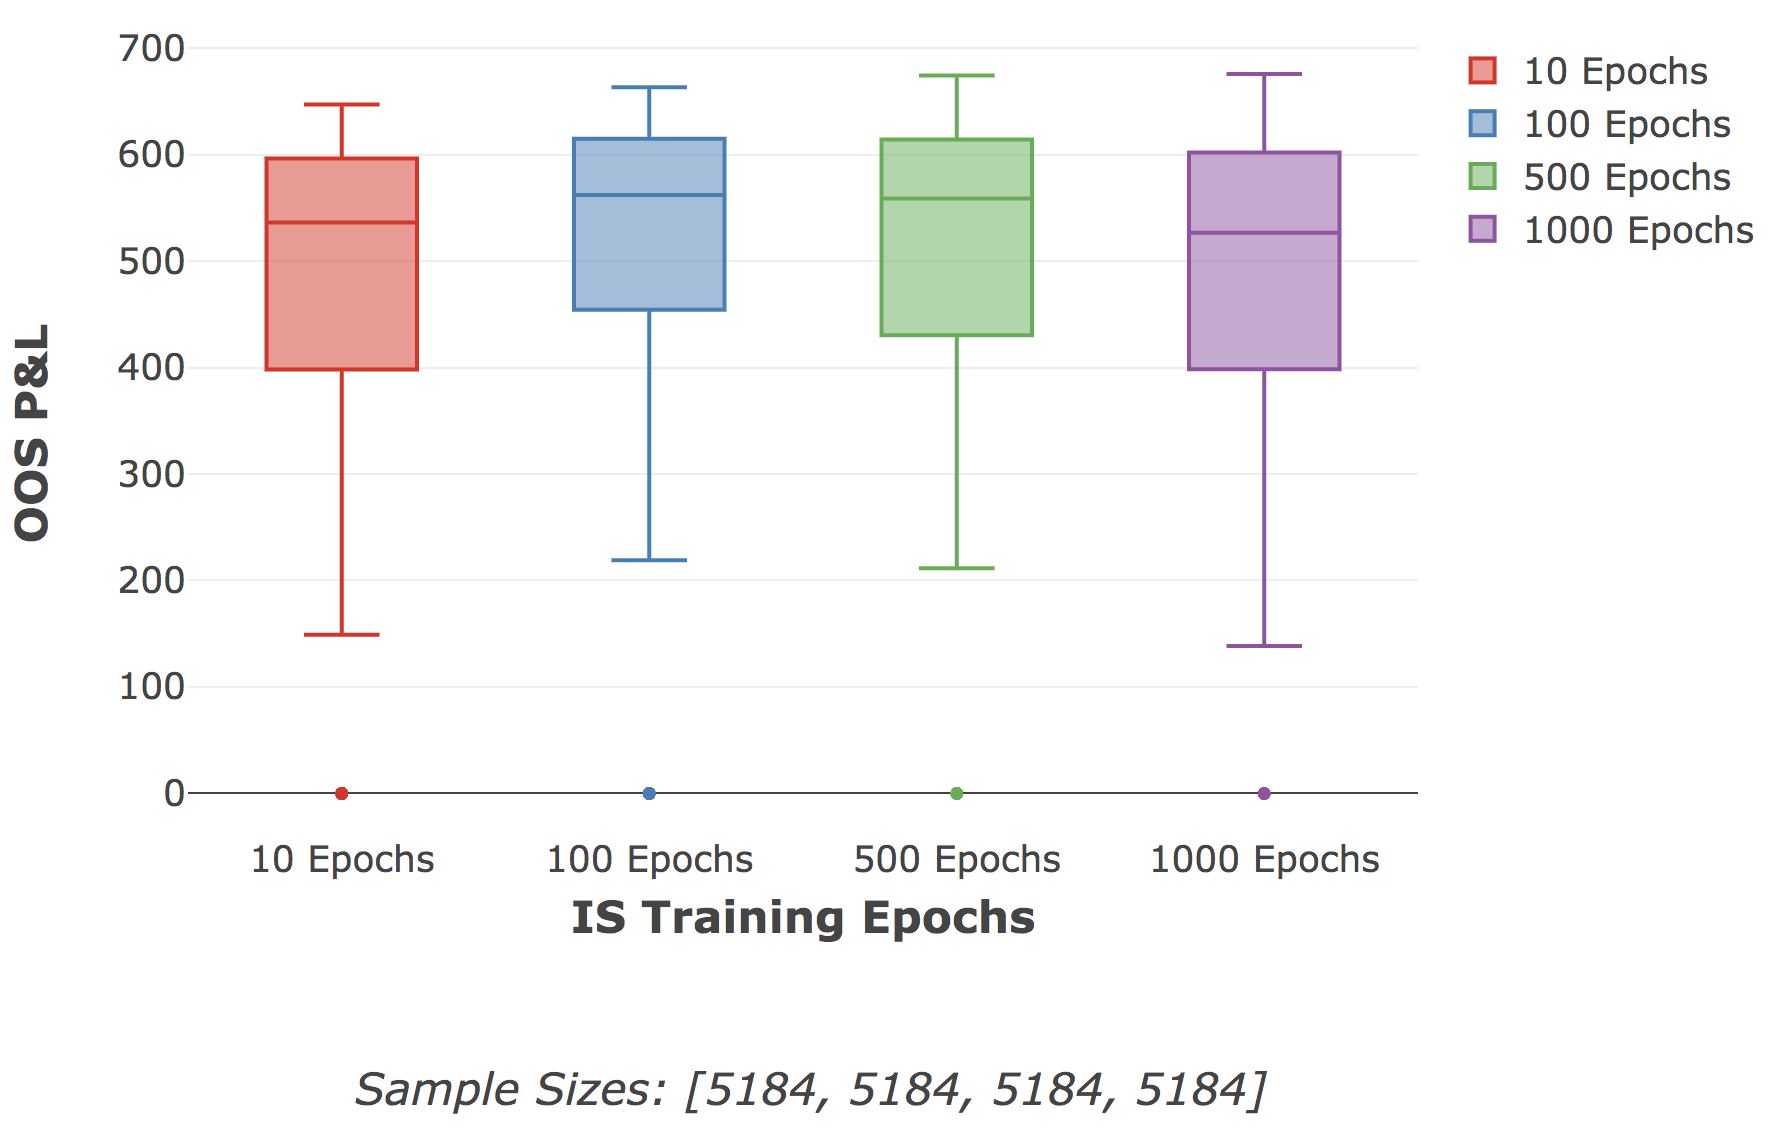
\includegraphics[scale=0.4]{images/results/8_3_historical/max_epochs.png}
		\caption[OOS P\&L by IS Training Epochs]
		{
			Dataset: Actual10 dataset (\ref{dataset_actual10}), Configuration 13 (\ref{config13}) 
			\newline The box plots above show OOS P\&L grouped by the number of epochs in the SGD IS training phase (i.e. the number of times the IS data was trained on). In this set of configurations, 100 Epochs offered the best overall performance, and further training to 500 or 1000 epochs degraded performance due to the network overfitting on the IS data. The results here are noteworthy as they show that the benefit of historical data is limited - having a network become better at learning return relationships from 10 years ago did not lead to increased OOS P\&L for more current data. The small difference in the upper half of observations between 10 and 100 Epochs further emphasises this point.
		}
		\label{figure-results_pl_max_epochs}
	\end{figure}
	
	
	\begin{figure}[H]
		\centering 
		\textbf{OOS P\&L by IS Training Dataset Size}
		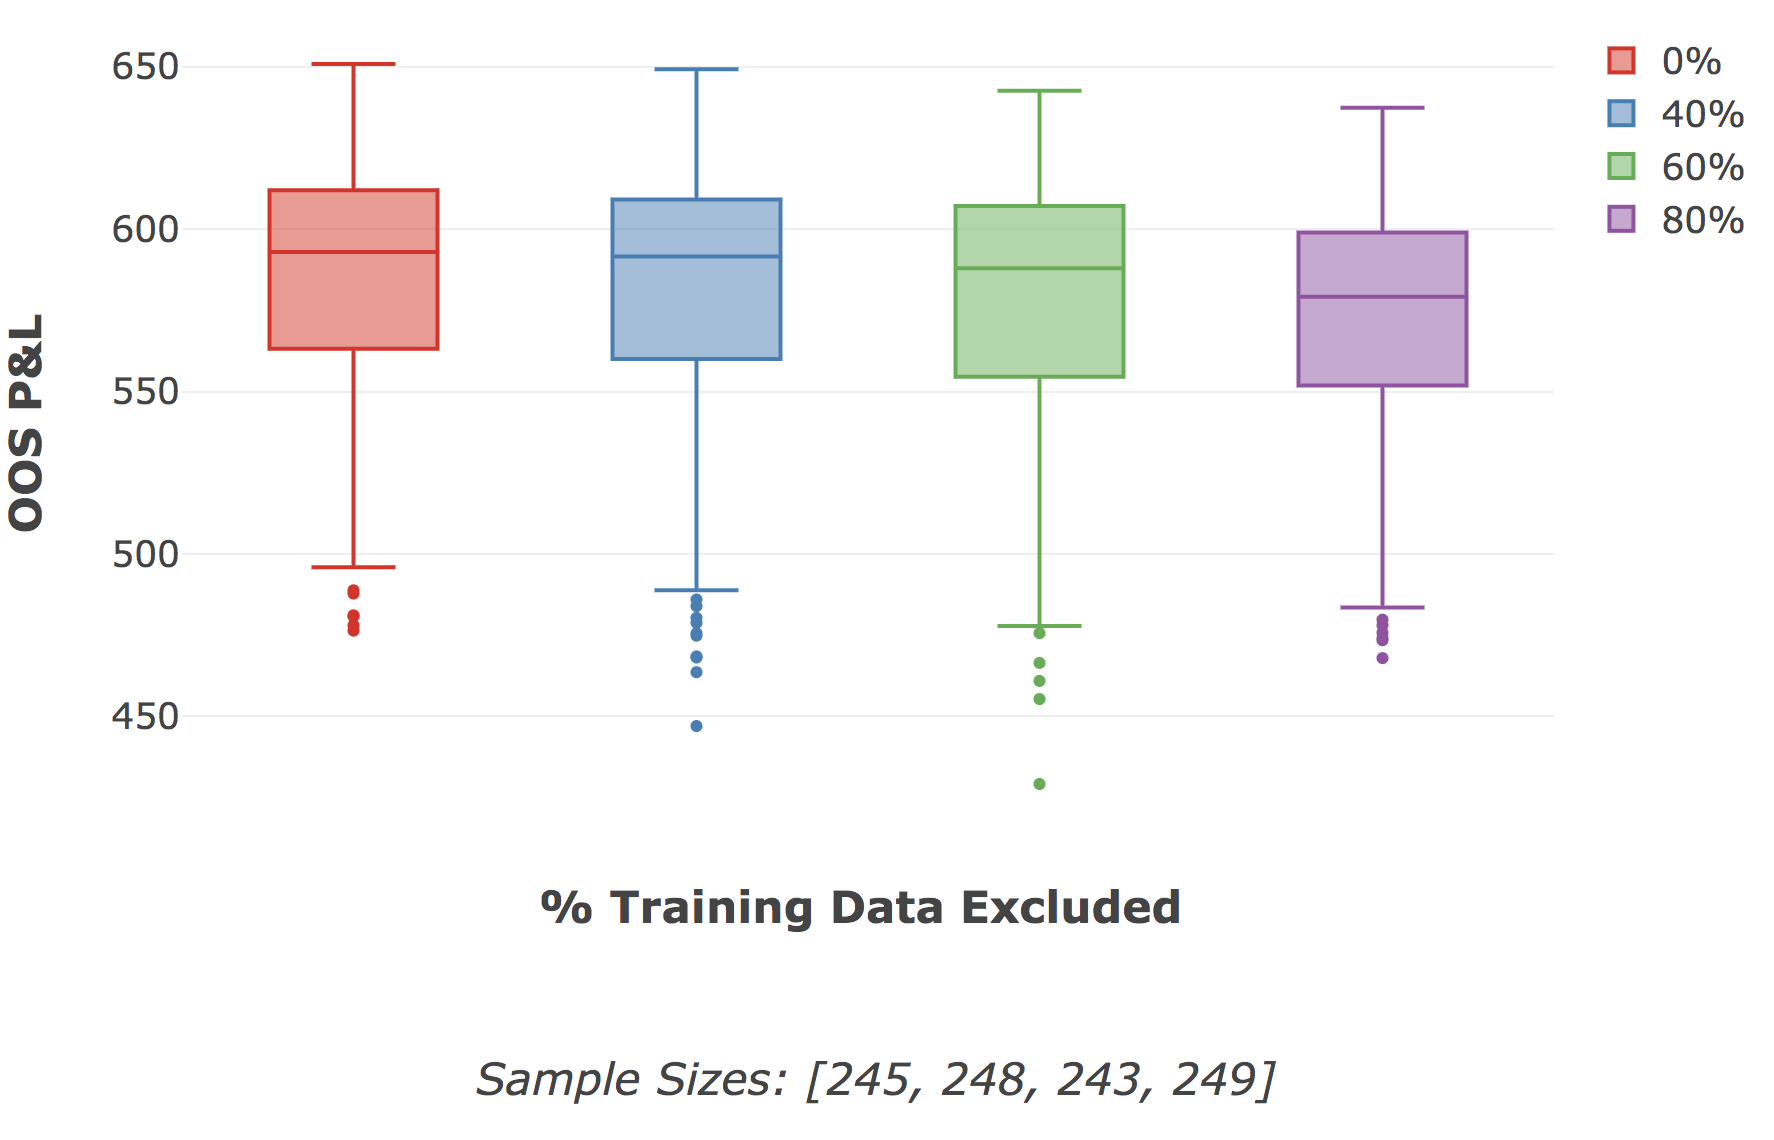
\includegraphics[scale=0.4]{images/results/8_3_historical/training_data_excluded.png}
		\caption[OOS P\&L by IS Training Dataset Size]{
			Dataset: Actual10 dataset (\ref{dataset_actual10}), Configuration 16 (\ref{config16}) (some samples with 0 P\&L were excluded for more effective visualization)
			\newline To further explore the effect of IS training on historical data, configurations were run with a percentage of the usual training data excluded, with the P\&L results grouped above. The exclusion of up to 80\% of the IS training data resulted in only a 2.2\% drop in median OOS P\&L for those networks. The training in these instances was not adjusted to increase the number of epochs according to the size of IS data, and so the configurations with more data excluded were also in essence trained less. These results, combined with those in Figure \ref{figure-results_pl_max_epochs} show the limited use in training on historical data, and hence the far greater value in current cross sectional information.}
		\label{figure-results_it3_validationset}
	\end{figure}
	
	
	\newpage
	
	\subsection{Weight Initializaton Techniques}\label{results_init}
	
	Neural network weight initialization has been one of the primary barriers to effective deep learning, with incorrect initializations leading to poor learning performance in deep networks. New techniques for initializing weights were one of the main reasons for the progress in the field \citep{Hinton2}. In Sections \ref{results_oos_pl} and \ref{results_data_hist}, we show that historical data and training are of limited value. The most profitable models learn quickly from recent data, and have had less training on historical data. The issue of weight initialization then is even more prominent when in the context of financial time series. The two most popular methods, RBM pre-training and variance based initialization, have both been explored and detailed below.
	
	\subsubsection{RBM Pretraining for Sigmoid Networks}
	
	While previously considered the best approach for training deep neural networks, we found that the methodology of greedy layerwise RBM pre-training for Sigmoid SAE networks (as described by \citet{Hinton2}) had detrimental effects on network performance, as seen in Figure \ref{figure-results-pretraining-effect}. \newline
	
	\begin{figure}[H]
		\centering
		\textbf{Pre-training Effects on SAE MSE Scores} 
		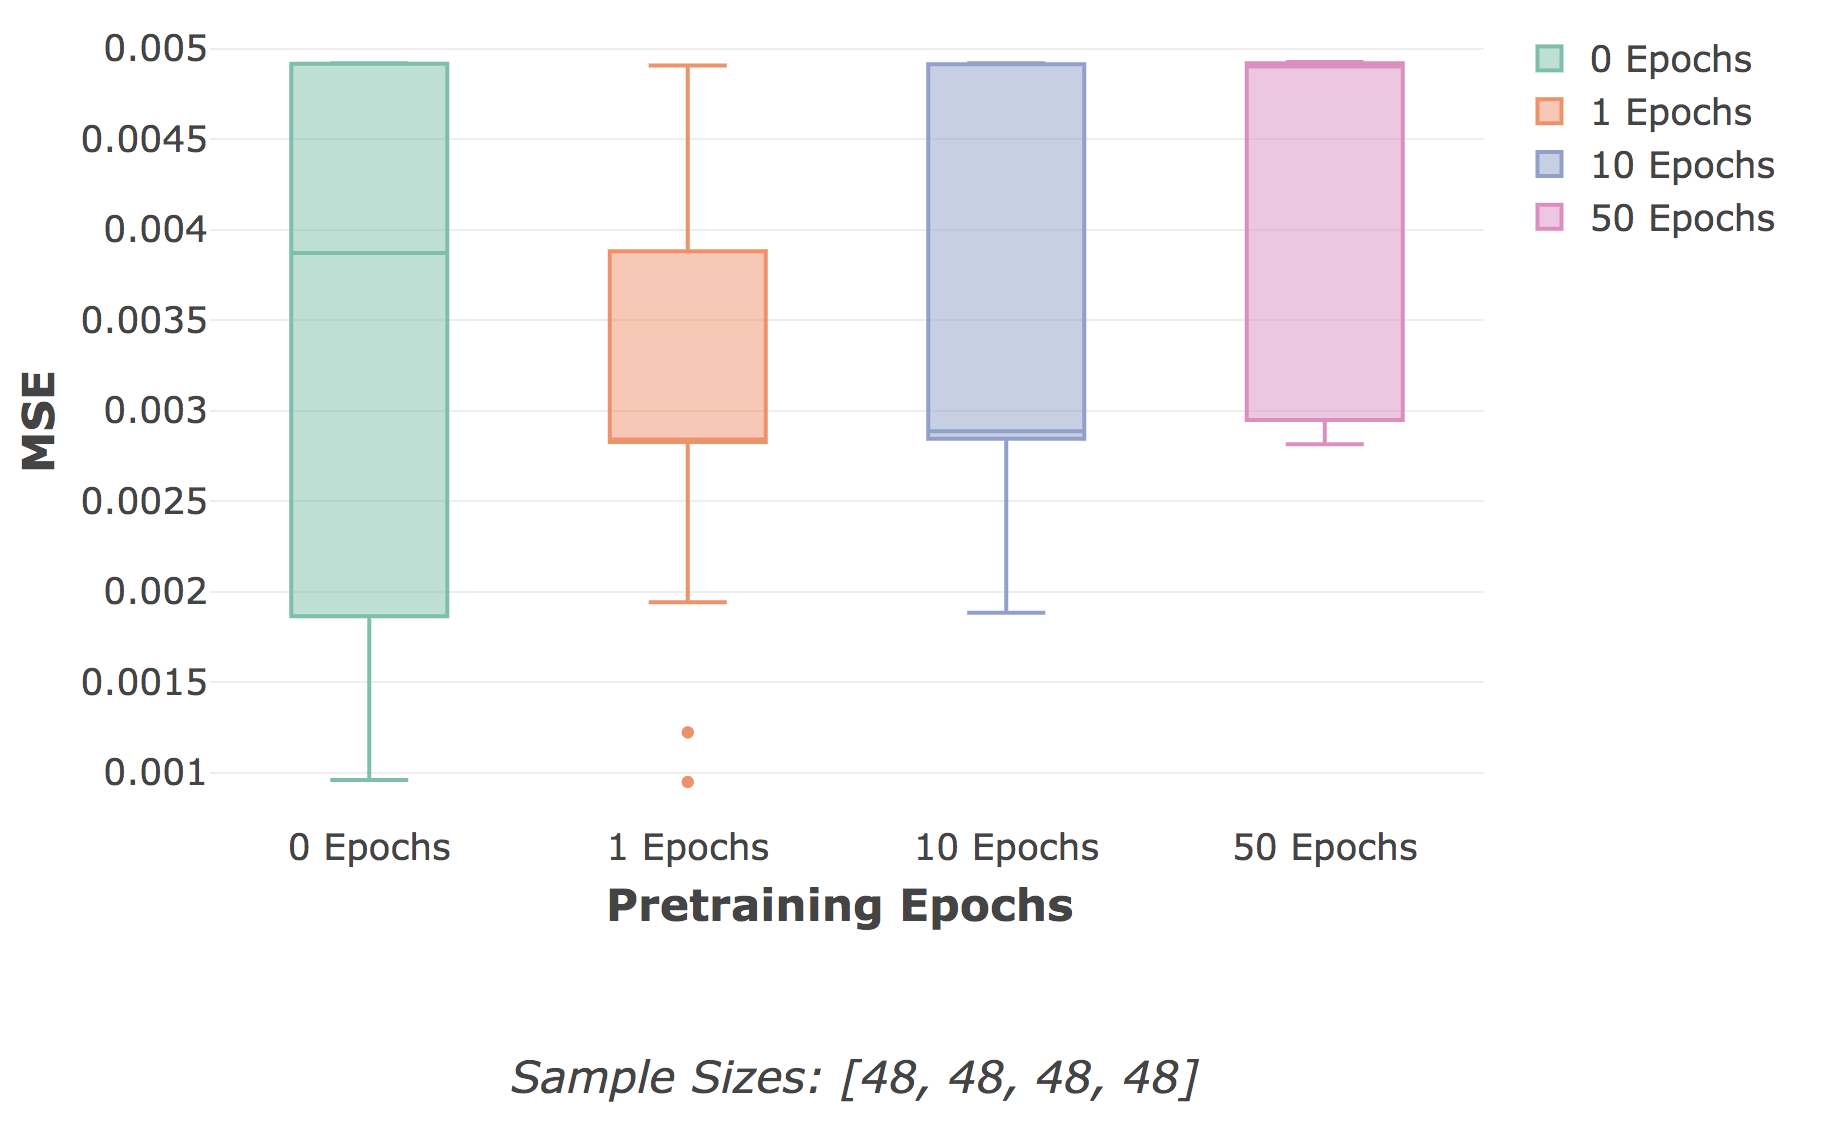
\includegraphics[scale=0.45]{images/results/8_4_weight_init/actual_sigmoid_pt.png}
		\caption[Pre-training Effects on SAE MSE Scores]
		{Dataset AGL\&ACL (\ref{dataset_aglacl}); Configuration 6 (\ref{config6})
			\newline \newline The boxplots here show the summary of configuration performances, by minimum MSE achieved, grouped according to the number of pre-training epochs. There was an evident benefit to having no pre-training in this scenario as there was a clear decrease in performance as the number of epochs increased (the low value outliers that can be seen for the 1 epoch configuration were with learning rates which were low enough to approximate no epochs).}
		\label{figure-results-pretraining-effect}
	\end{figure}		
	
	The RBM pre-training technique does assume that data is Independent and Identically Distributed (IID), and does ultimately traverse a different solution space and loss function. While it may be effective in some contexts, we saw it had a counterproductive exploration of the weight space for this non-IID dataset, and that ultimately the financial time series data is pathological for RBM pre-training. It may also again emphasise the value of more recent data over historical data\footnote{The RBM greedy layerwise training implementation was effectively tested and validated on known datasets such as MNIST, example results for which can bee seen in Section \ref{results_init_appendix} of the Appendix.}.\newline 
	
	\subsubsection{Variance Based Weight Initialization Techniques}
	
	More recent research has focused on the use of weight initialization using variance based methodologies, as discussed fully in Section \ref{imp_weights}. Our expectation, theoretically, was that the He initialization would generally outperform Xavier due to it being more appropriate for the ReLU activations being used. Additionally, in networks with varying layer sizes, we expected He-Adj and possibly Xavier to outperform He which is subject to imbalanced initializations. Ultimately, He-Adj as presented in Section \ref{imp_weights}, should present the best of both for an initialization that is suited to Leaky ReLU activations and the varying layer sizes found in SAE networks.\newline
	
	\begin{figure}[H]
		\centering
		\textbf{SAE MSE by Weight Initialization}
		\begin{subfigure}{.5\textwidth}
			\centering 
			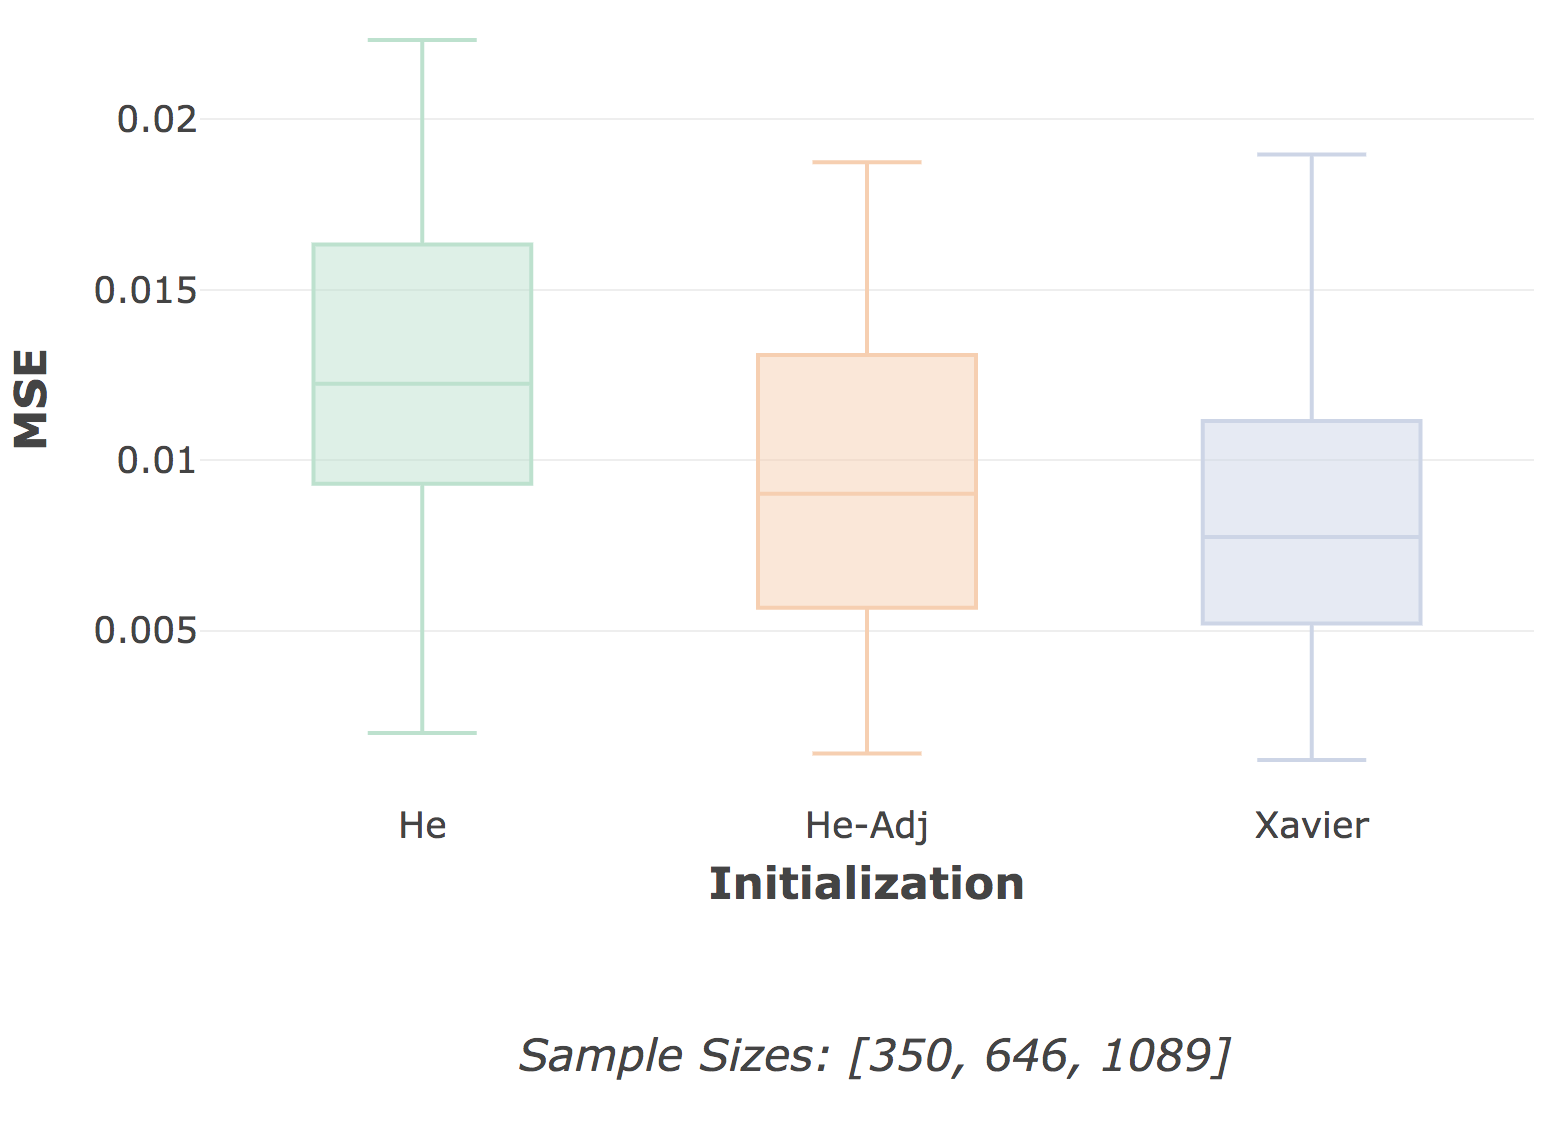
\includegraphics[scale=0.29]{images/results/8_4_weight_init/synthetic_mse_init.png}
			\caption{\textbf{Synthetic Data} 
				\newline }
			\label{figure-synthetic_mse_init}
		\end{subfigure}%
		\begin{subfigure}{.5\textwidth}
			\centering 
			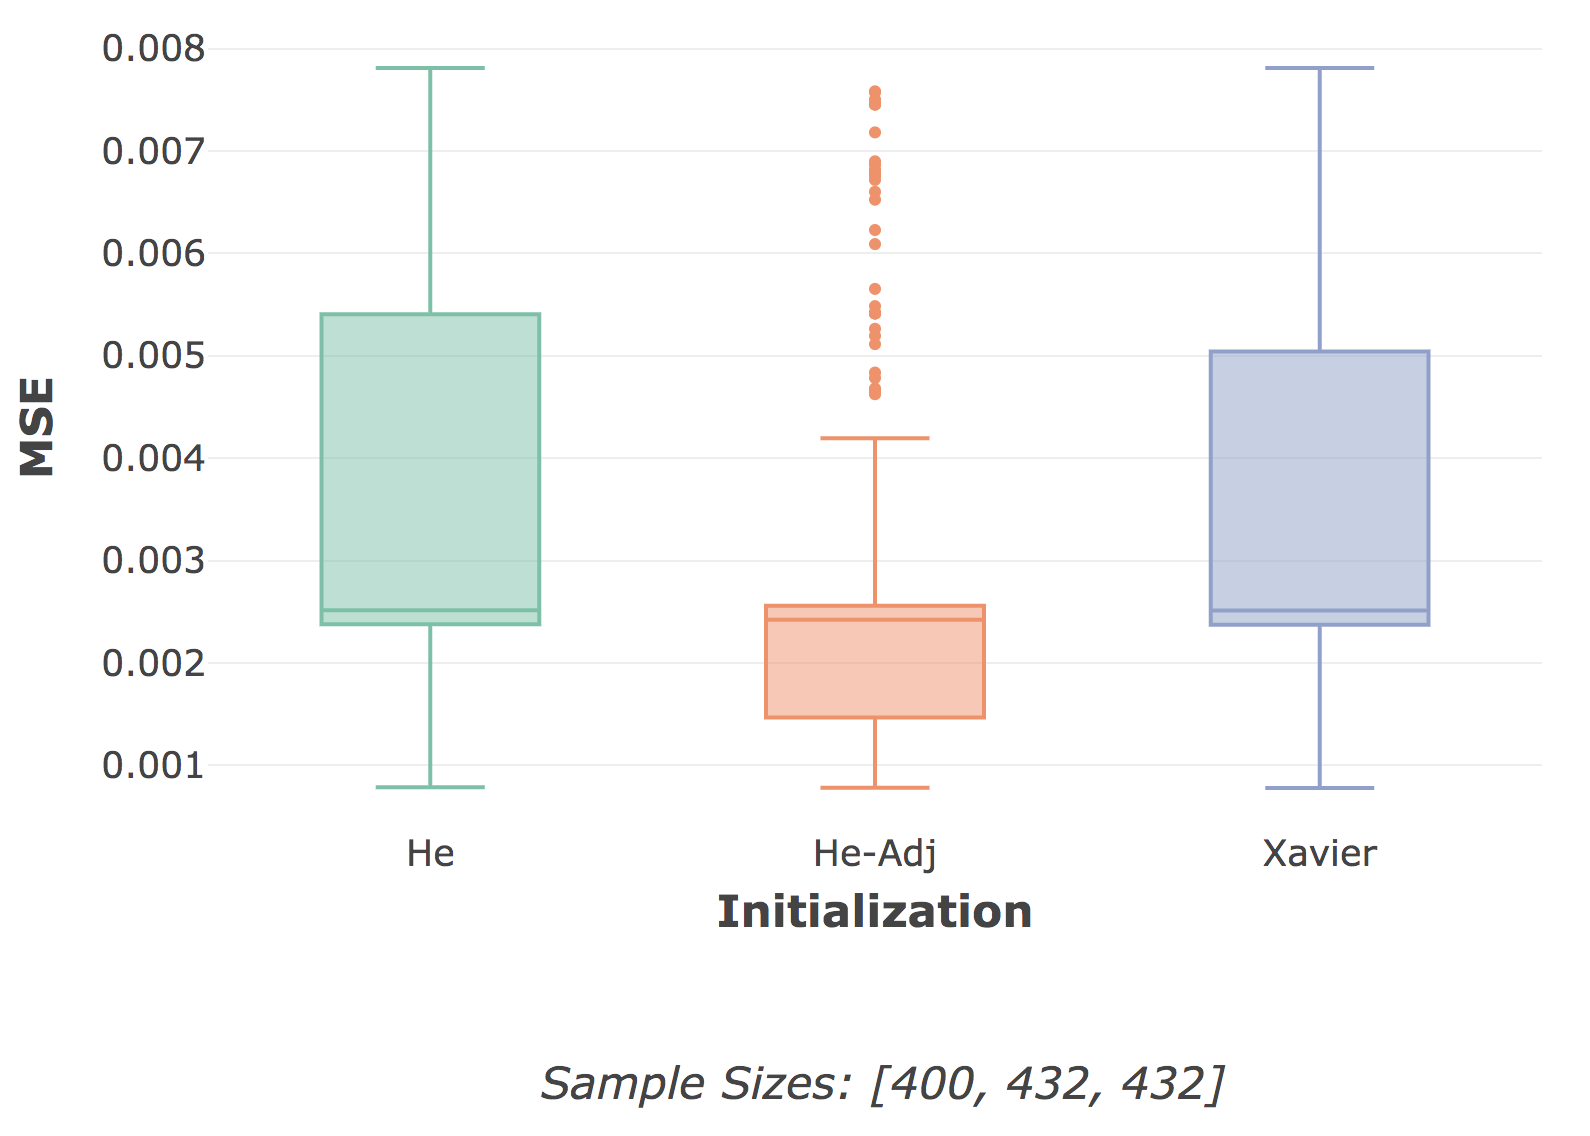
\includegraphics[scale=0.28]{images/results/8_4_weight_init/agl_mse_init.png}
			\caption{\textbf{AGL} 
				\newline }
			\label{figure-agl_mse_init}
		\end{subfigure}
		\caption[SAE MSE by Weight Initialization]
		{Dataset: Synthetic10 (\ref{dataset_synthetic10}), AGL (\ref{dataset_agl}), Configuration 7 (\ref{config7}) \& Configuration 8 (\ref{config8})
			\newline Training SAE networks across the Synthetic10 and AGL  datasets, we mostly saw the expected patterns emerge. He-Adj consistently outperformed He due to being better suited to the network structures, as seen in the plots above. We also saw that He-Adj clearly outperforms Xavier for AGL data, but has performance that was mostly the same (or even marginally worse) than Xavier for the synthetic dataset. Similar trends as AGL were seen when SAEs were trained for the full 10 asset dataset, which can be see in Appendix \ref{results_init_appendix}.}
		\label{figure-mse_init}
	\end{figure}
	
	
	\begin{figure}[H]
		\centering
		\textbf{OOS P\&L by Weight Initialization}
		\begin{subfigure}{.5\textwidth}
			\centering 
			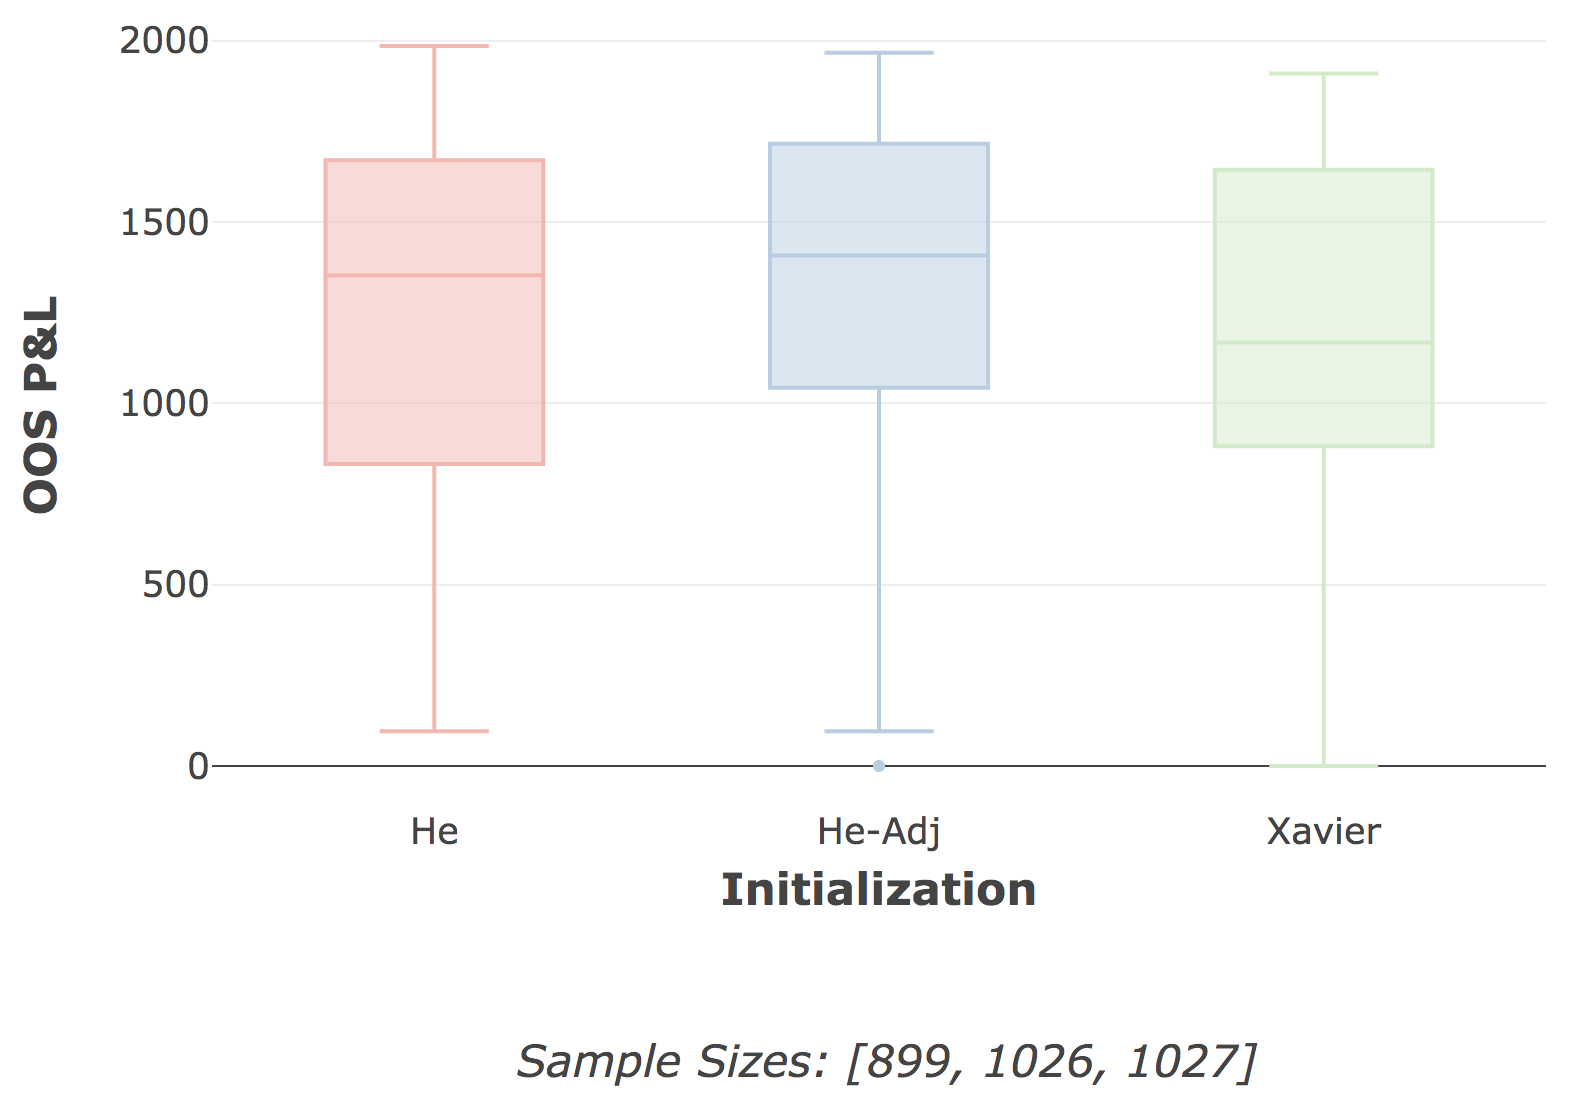
\includegraphics[scale=0.28]{images/results/8_4_weight_init/synth_pl_init.png}
			\caption{\textbf{Synthetic Data} 
				\newline }
			\label{figure-synthetic_pl_init}
		\end{subfigure}%
		\begin{subfigure}{.5\textwidth}
			\centering 
			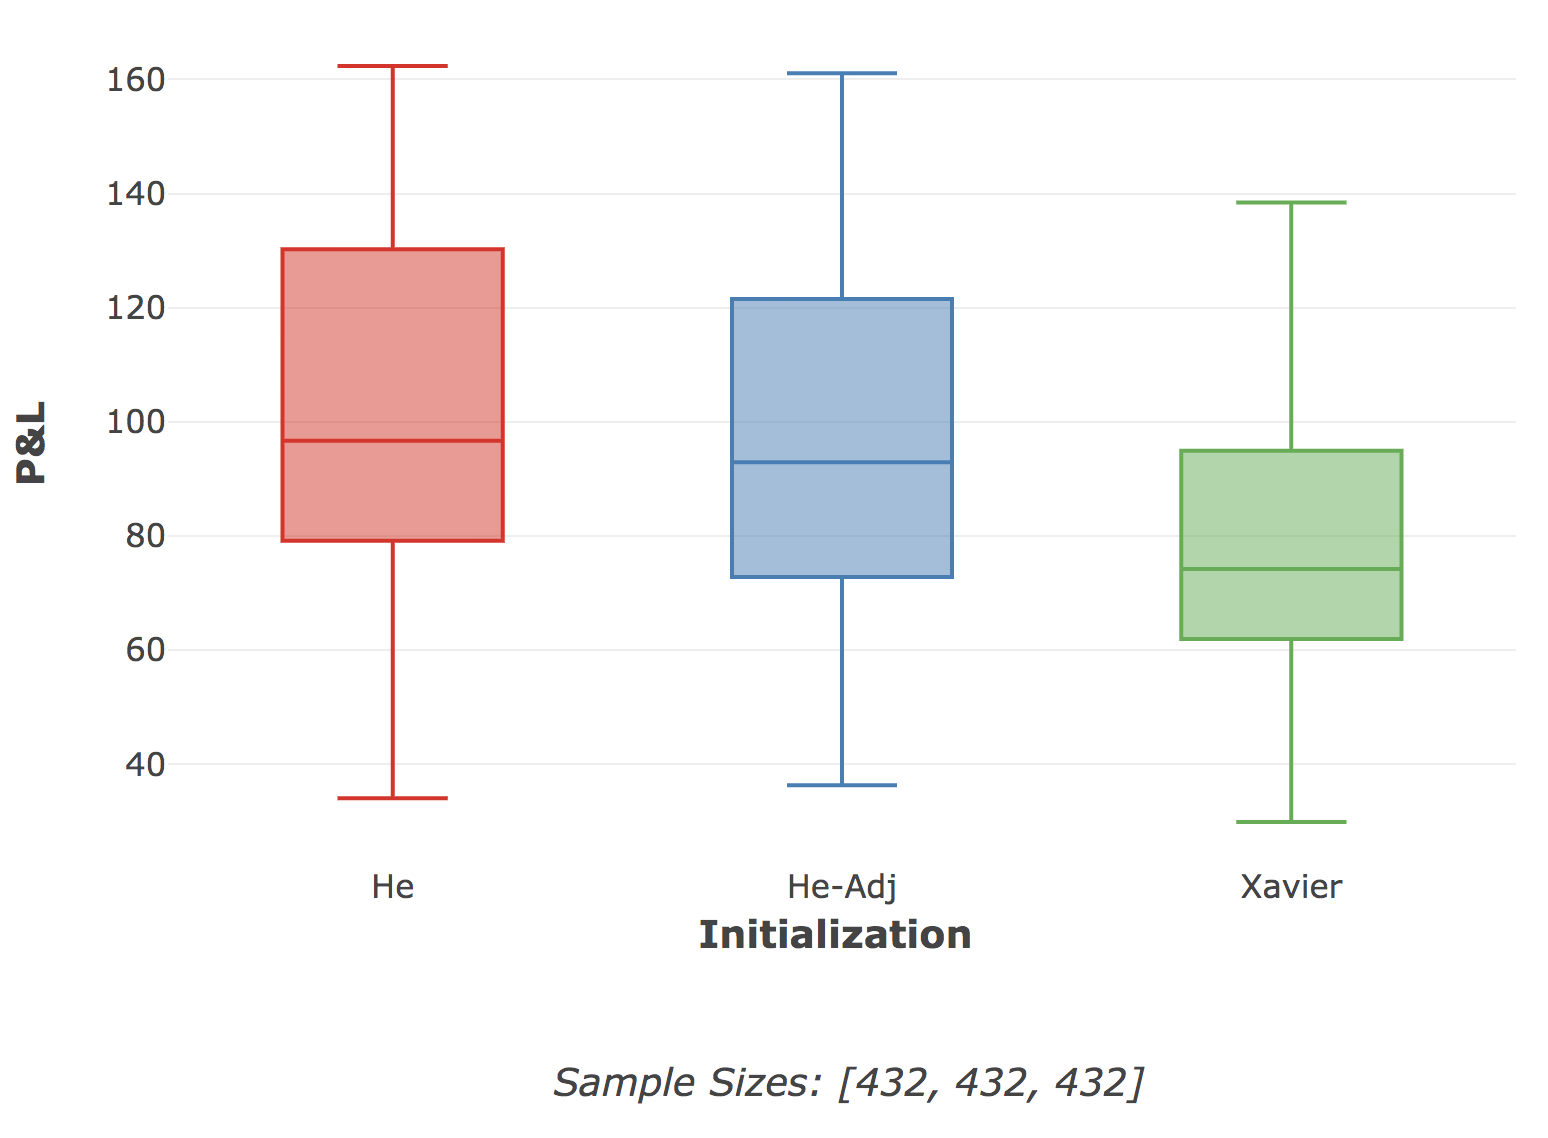
\includegraphics[scale=0.28]{images/results/8_4_weight_init/agl_pl_init.png}
			\caption{\textbf{AGL} 
				\newline }
			\label{figure-agl_pl_init}
		\end{subfigure}
		\caption[OOS P\&L by Weight Initialization]
		{Dataset: Synthetic10 (\ref{dataset_synthetic10}), AGL (\ref{dataset_agl}), Configuration 9 (\ref{config9}) \& Configuration 10 (\ref{config10})
			\newline Figure (a) shows OOS P\&L performance for synthetic data. The networks with more consistent layer sizes resulted in the performance between He and He-Adj becoming comparable, while both outperformed Xavier (as expected, with ReLU activations). In Figure (b), the P\&L results for AGL data had clear outperformance of Xavier by the He based initializations, but a less clear comparison between He and He-Adj.}
		\label{figure-pl_init}
	\end{figure}
	
	The results here mostly conformed to the theoretical expectations, though there are some inconsistencies. As discussed more fully in Section \ref{results_synth}, the GBM data in synthetic datasets will have assets that are configured to certain mean and variances. As these movements are processed, scaled and aggregated over time through the data processing, the movements will generally be more similar and less complex than those of actual stock data which will show greater variance over time (this is shown more concretely in Figure \ref{figure-actual_aggregate_dist}). The learning process then is not required to be able to pass through error signals that change as dynamically over time, and so there is less pressure on the initial starting weights. This consideration may account for the unexpected performance of the Xavier initialization in the Synthetic SAE networks. Further, some of the assumptions of these techniques, such as data being IID, may not apply in the first place, making their results less predictable.  Due to the generally better or comparable performance of He-Adj, it was the only initialization chosen for further trials.  \newline
	
	\newpage
	\subsection{Synthetic Data}\label{results_synth}
	
	\subsubsection{GBM Generated Data}\label{results_gbm_data}
	
	Geometric Brownian Motion (GBM), as discussed in Section \ref{data_synthetic}, was used to simulate synthetic datasets for the purposes of testing implementations and configurations without influencing the likelihood of backtest overfitting. GBM is a popular choice for synthetic financial data as it is a Markov process, thus following a random walk and is generally consistent with the efficient market hypothesis in that the next price movement is conditionally independent of past movements. In line with this though, the series will exhibit a constant drift with price shocks according to its stationary configuration, and changes in price follow a particular distribution. It is worth noting that as GBM time series are non-ergodic, one should be wary of considering ensemble based predictions with much confidence \citep{Peters}. GBM generated data provides a valuable tool in assessing ideas without taking on any risks, but these results need to be considered correctly. \newline
	
	This section details how the behaviour of synthetic data differed from actual data in some of the more critical areas of our experimentation process.
	
	\subsubsection{Synthetic Data Horizon Effects}\label{results_synthdata_mse}
	
	\begin{figure}[H]
		\centering
		\textbf{SAE MSE Scores for Synthetic Data}
		\begin{subfigure}{.99\textwidth}
			\centering 
			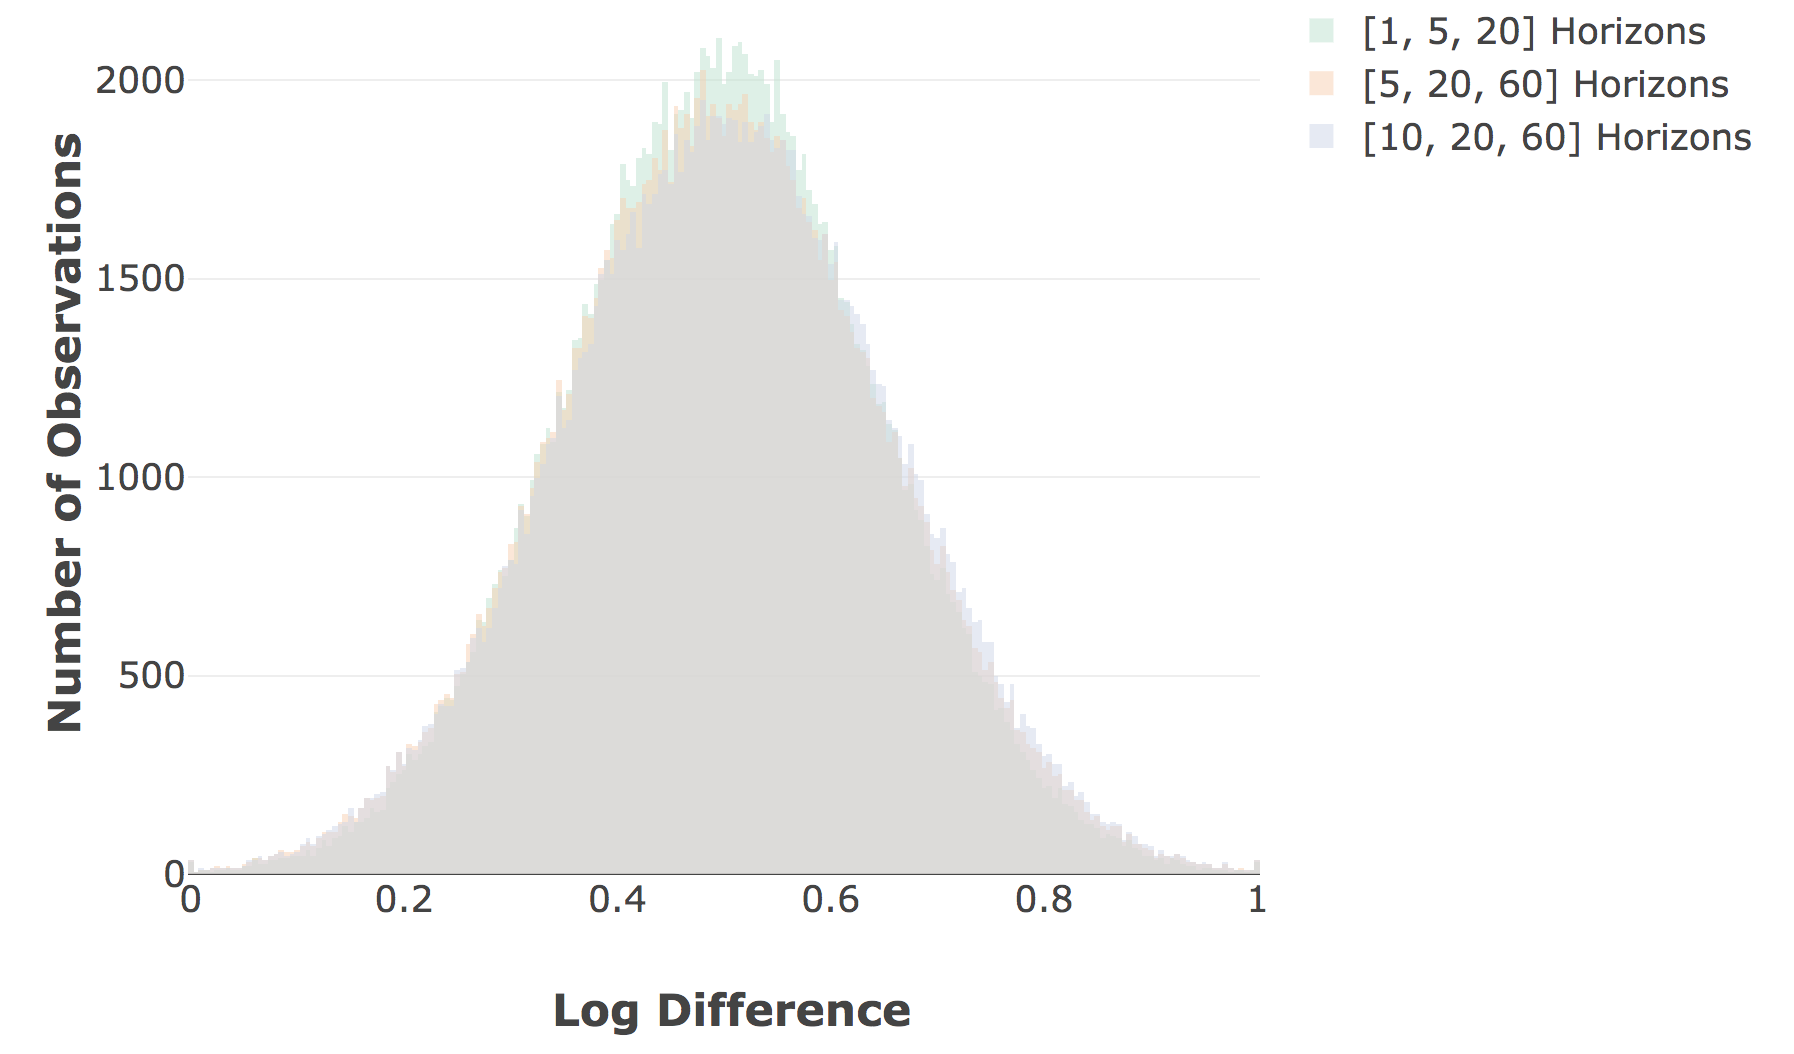
\includegraphics[scale=0.4]{images/results/8_5_synthetic_data/test_aggregate_dist.png}
			\caption{\textbf{Log Difference Distributions} 
				\newline }
			\label{figure-test_aggregate_dist}
		\end{subfigure}
		\begin{subfigure}{.99\textwidth}
			\centering 
			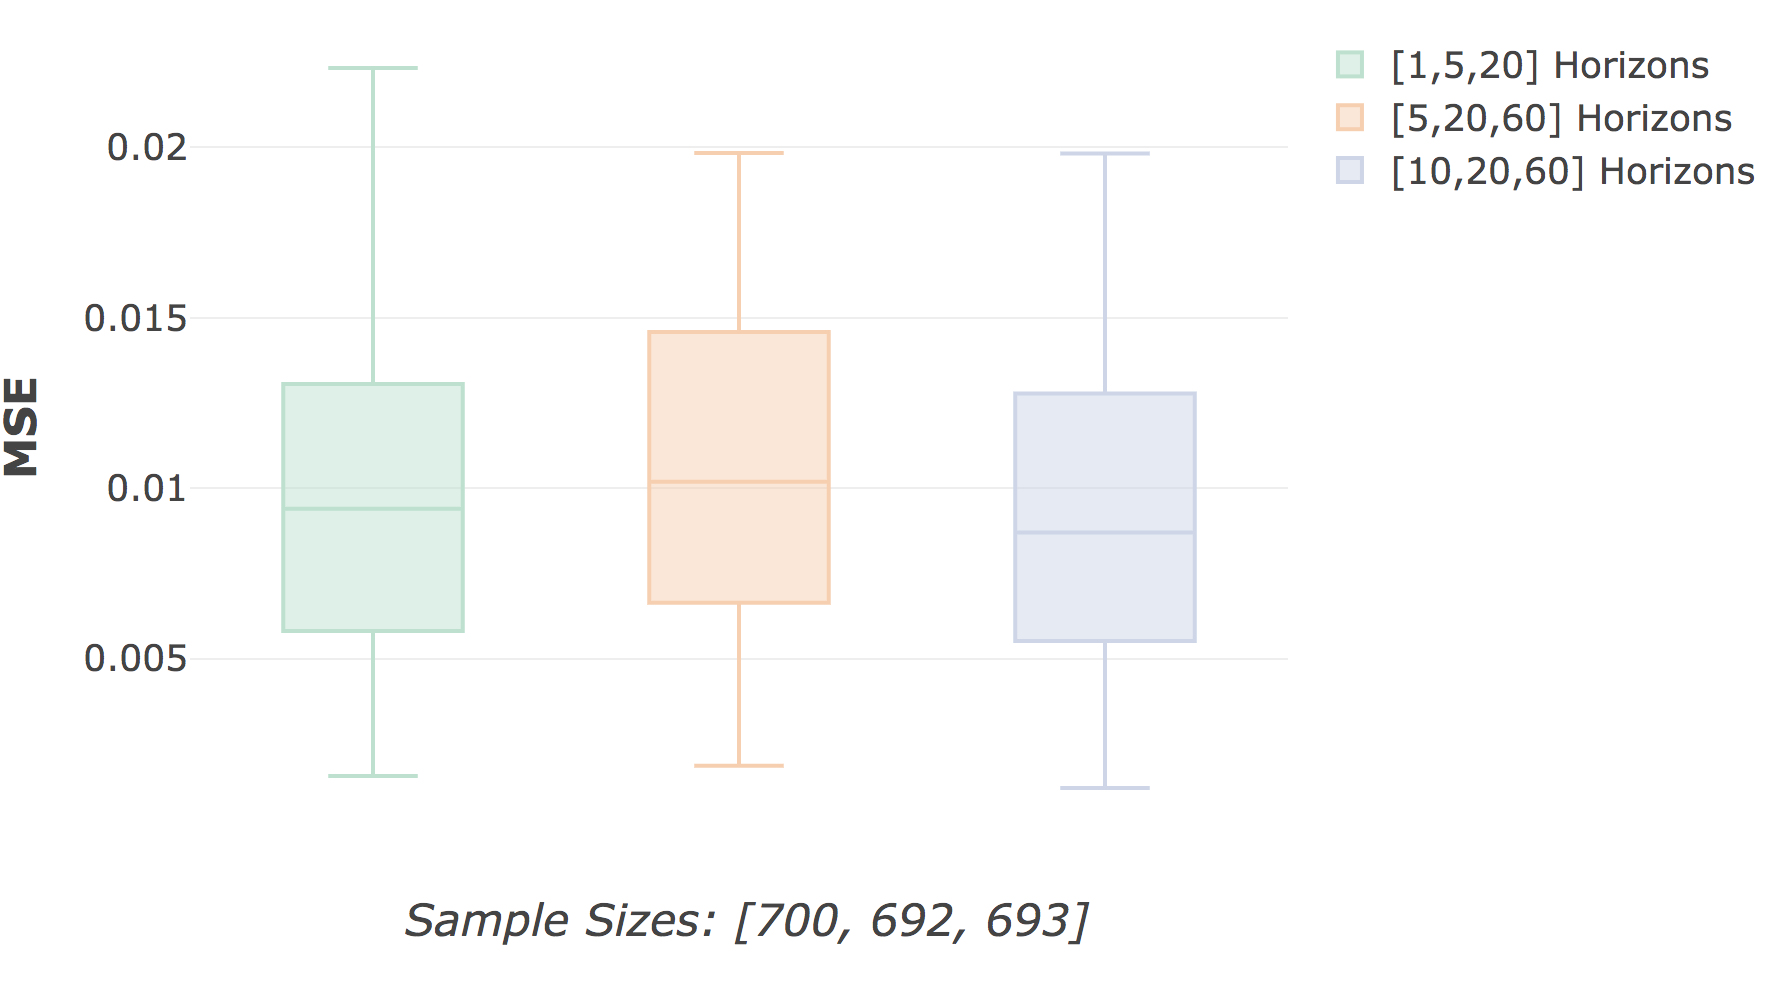
\includegraphics[scale=0.4]{images/results/8_5_synthetic_data/test_aggregation_mse.png}
			\caption{\textbf{SAE MSE Scores} 
				\newline }
			\label{figure-test_aggregation_mse}
		\end{subfigure}
		\caption[SAE MSE Scores for Synthetic Data]
		{Dataset: Synthetic10 dataset (\ref{dataset_synthetic10}), Configuration 7 (\ref{config7})
			\newline Figure (a) shows the distribution of values to be replicated by the SAE for synthetic data. Geometric Brownian Motion generates discrete changes that follow a log-normal distribution, the log difference and scaling of which (as per the data processing described in Section \ref{data_processing}) result in normally distributed price changes. We see small differences in the distributions according to the data horizons used, as one would expect, with slightly lower variances occurring for smaller data horizons ($\sigma_{[1,5,20]} = 0.145$, $\sigma_{[5,20,60]} = 0.152$, $\sigma_{[10,20,60]} = 0.154$). There were some differences in SAE performance as indicated in Figure (b), though not to large extents and considering the very similar distribution of values, there was not any expectation of seeing fundamental differences in the networks ability to compress and replicate them. 
			\newline Figure \ref{fig_data_sae_actual} shows the equivalent for actual data, where there is a significant difference in variances for longer data horizons which are more difficult to replicate.}
		\label{figure-data_sae_synthetic}
	\end{figure}
	
	
	
	\begin{figure}[H]
		\centering 
		\textbf{OOS P\&L by Data Horizon (Synthetic Data)}
		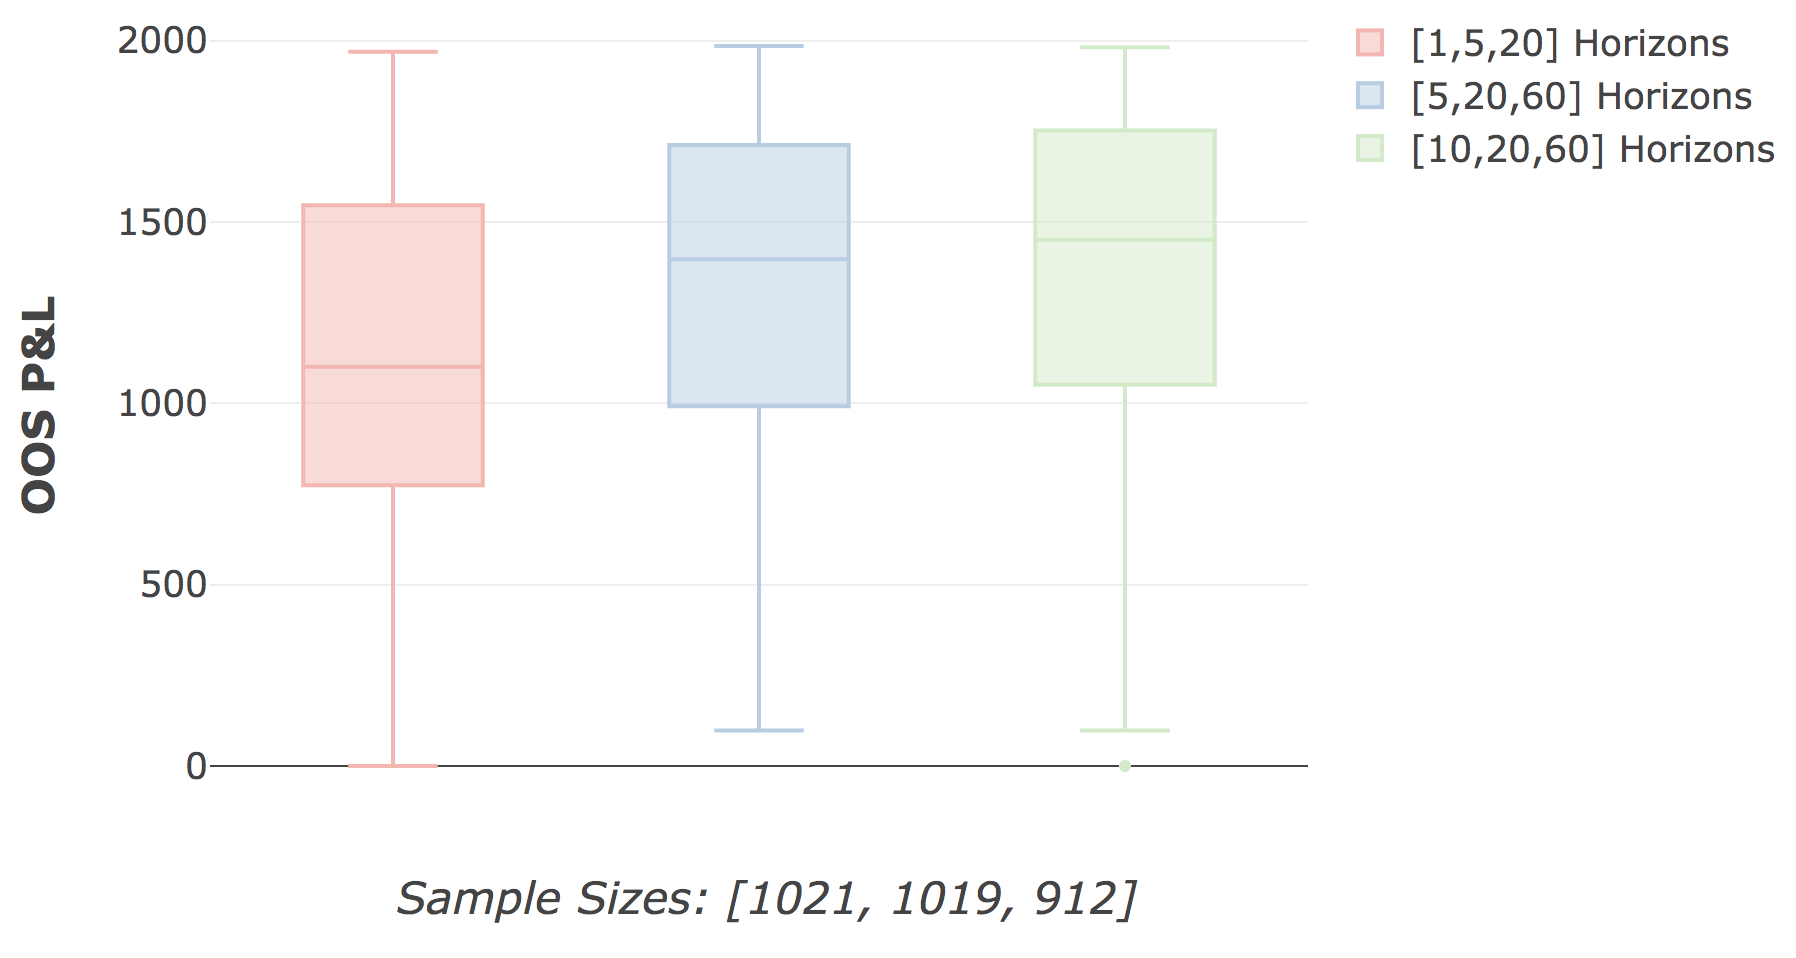
\includegraphics[scale=0.36]{images/results/8_5_synthetic_data/test_aggregation_pl.png}
		\caption[OOS P\&L by Data Aggregation for Synthetic Data]{
			Dataset: Synthetic10 dataset (\ref{dataset_synthetic10}), Configuration 9 (\ref{config9})
			\newline  The boxplots here show the P\&L from the MMS grouped by the data horizon configurations. There was a clear trend of P\&L increasing as the length of the windows increased. Shorter term GBM data would be more likely to represent fluctuations, whereas the longer term windows will be more representative of the constant mean in the asset price fluctuations, leading to easier predictive performance and higher P\&L. This is in clear contrast to the effects seen in actual data, where both long term and short term strategies are present, with the highest P\&L occurring for shorter horizon aggregations (these can be seen in Figure \ref{figure-actual_aggregation_pl}).}
		\label{figure-test_aggregation_pl}
	\end{figure}
	
	\begin{figure}[H]
		\centering 
		\textbf{OOS P\&L by Feature Selection Size and OGD Learning Rate}
		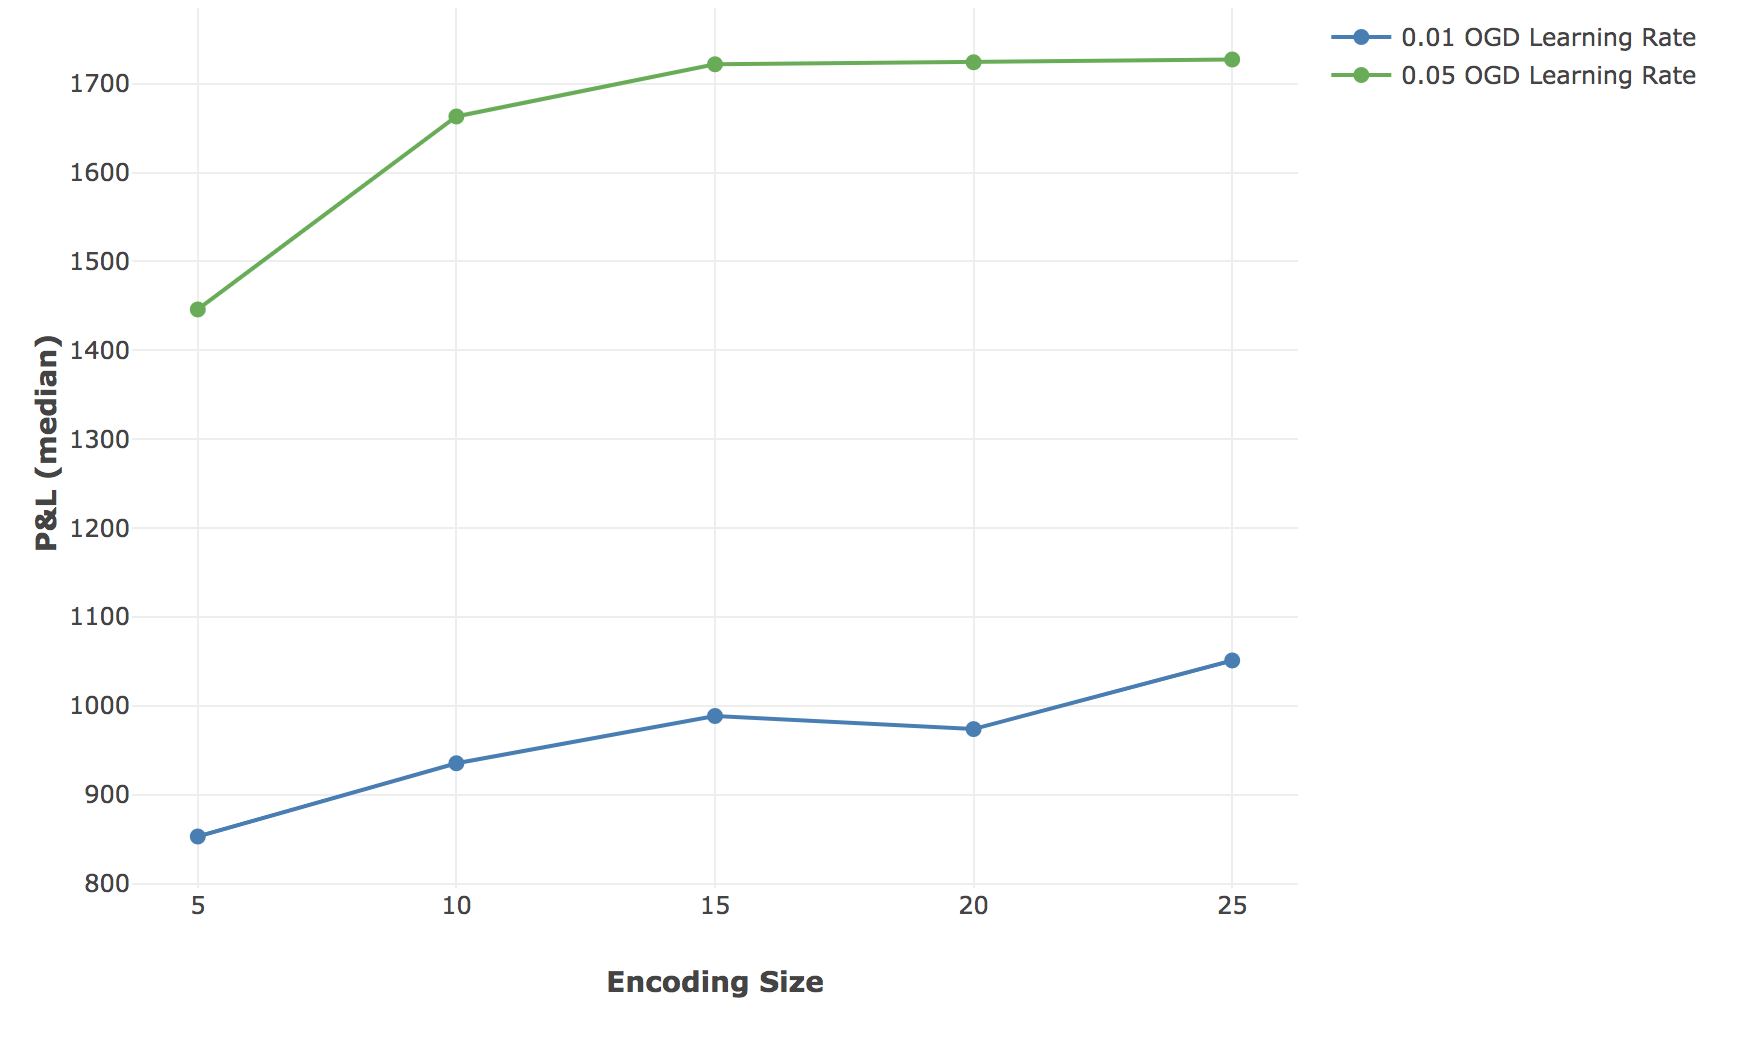
\includegraphics[scale=0.36]{images/results/8_5_synthetic_data/synthetic_median.png} 
		\caption[OOS P\&L by Feature Selection Size and OGD Learning Rate (Synthetic Data)]{Dataset: Synthetic10 (\ref{dataset_synthetic10}) ; Configurations 9 (\ref{config9})
			\newline The trends in the synthetic data were straightforward in comparison to actual data. Feature reduction is possible, with OOS P\&L increasing as encoding size increases. There is however an optimal point around 15, after which performance plateaus. Given the stabler nature of GBM data, this is to be expected. The results here offer a nice counterpoint to what is seen in the actual data. With the GBM data having constant characteristics throughout the whole dataset, there is no potential for the SAE to overfit to IS data and have a potentially detrimental effect as the learning rate increases (as was the case with actual data). Results for SAE MSE were largely the same, which can be seen in Appendix \ref{results_features_appendix}.
		}
		\label{figure-synthetic_median}
	\end{figure}
	
	\newpage
	
	
	
	
	
	
	
	
	
	
	
	\newpage
	
	\subsection{Complexity of Financial Time Series}\label{results_finance_data}
	
	The complex nature of financial markets, with a high noise to signal ratio and constantly changing dynamics, presents challenges during the learning process. A model's success lies in its ability to reduce noise without losing signal, and being able to capture determinant features of importance. This section considers how these issues affect data preparation in terms of scaling, and how SGD learning optimizations are able to help improve performance in SAE reproduction (Unsupervised Learning) and FFN prediction (Supervised Learning).
	
	\subsubsection{Data Scaling}
	
	We found the effects of different scaling techniques (Normalization and Standardization), as described in Section \ref{data_scaling}, had significant impacts on SAE performance as seen in Figure \ref{figure-actual_mse_scaling}. The suggested implementation of the limited scaling approaches for the FFN networks was tested on Synthetic data (seen in Figure \ref{figure-synth_pl_scaling}), showing a relatively small impact. The impact on FFN prediction is expected to be more significant when applied to actual data, which would contain unstable variances over time.
		
	\begin{figure}[H]
		\centering 
		\textbf{SAE MSE by Scaling Function}
		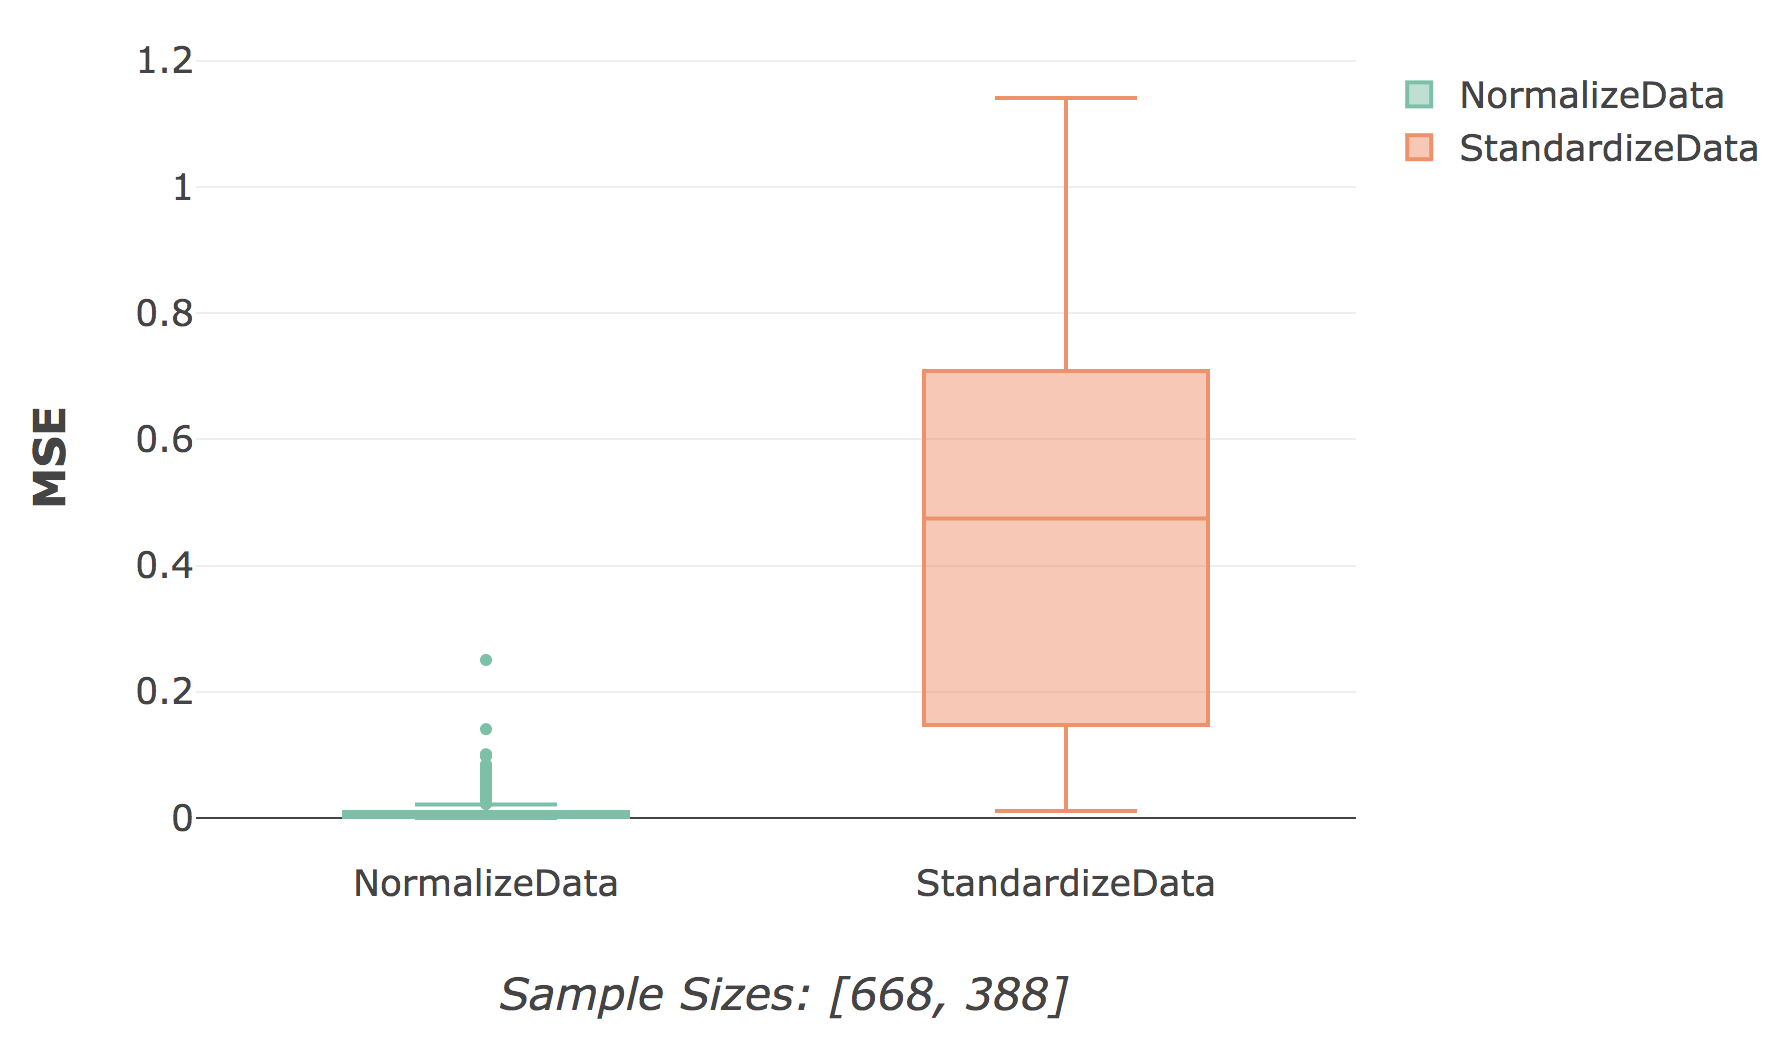
\includegraphics[scale=0.4]{images/results/8_6_complexity/mse_scaling.png}
		\caption[SAE MSE by Scaling Function]
		{Dataset: Scaling10 dataset (\ref{dataset_scaling10}), Configuration 1 (\ref{config1})
			\newline The figure here shows SAE MSE performance according to the scaling techniques as described in Section \ref{data_scaling}. As discussed in Section \ref{proc_dataprep}, the use of standardization for scaling the data does not allow for effective outlier treatments, resulting in the significantly worse performance seen. This again shows the difficulty of dealing with financial time series, which are likely to have many outliers.}
		\label{figure-actual_mse_scaling}
	\end{figure}

	\begin{figure}[H]
		\centering
		\textbf{OOS P\&L by Scaling (Synthetic Data)} 
		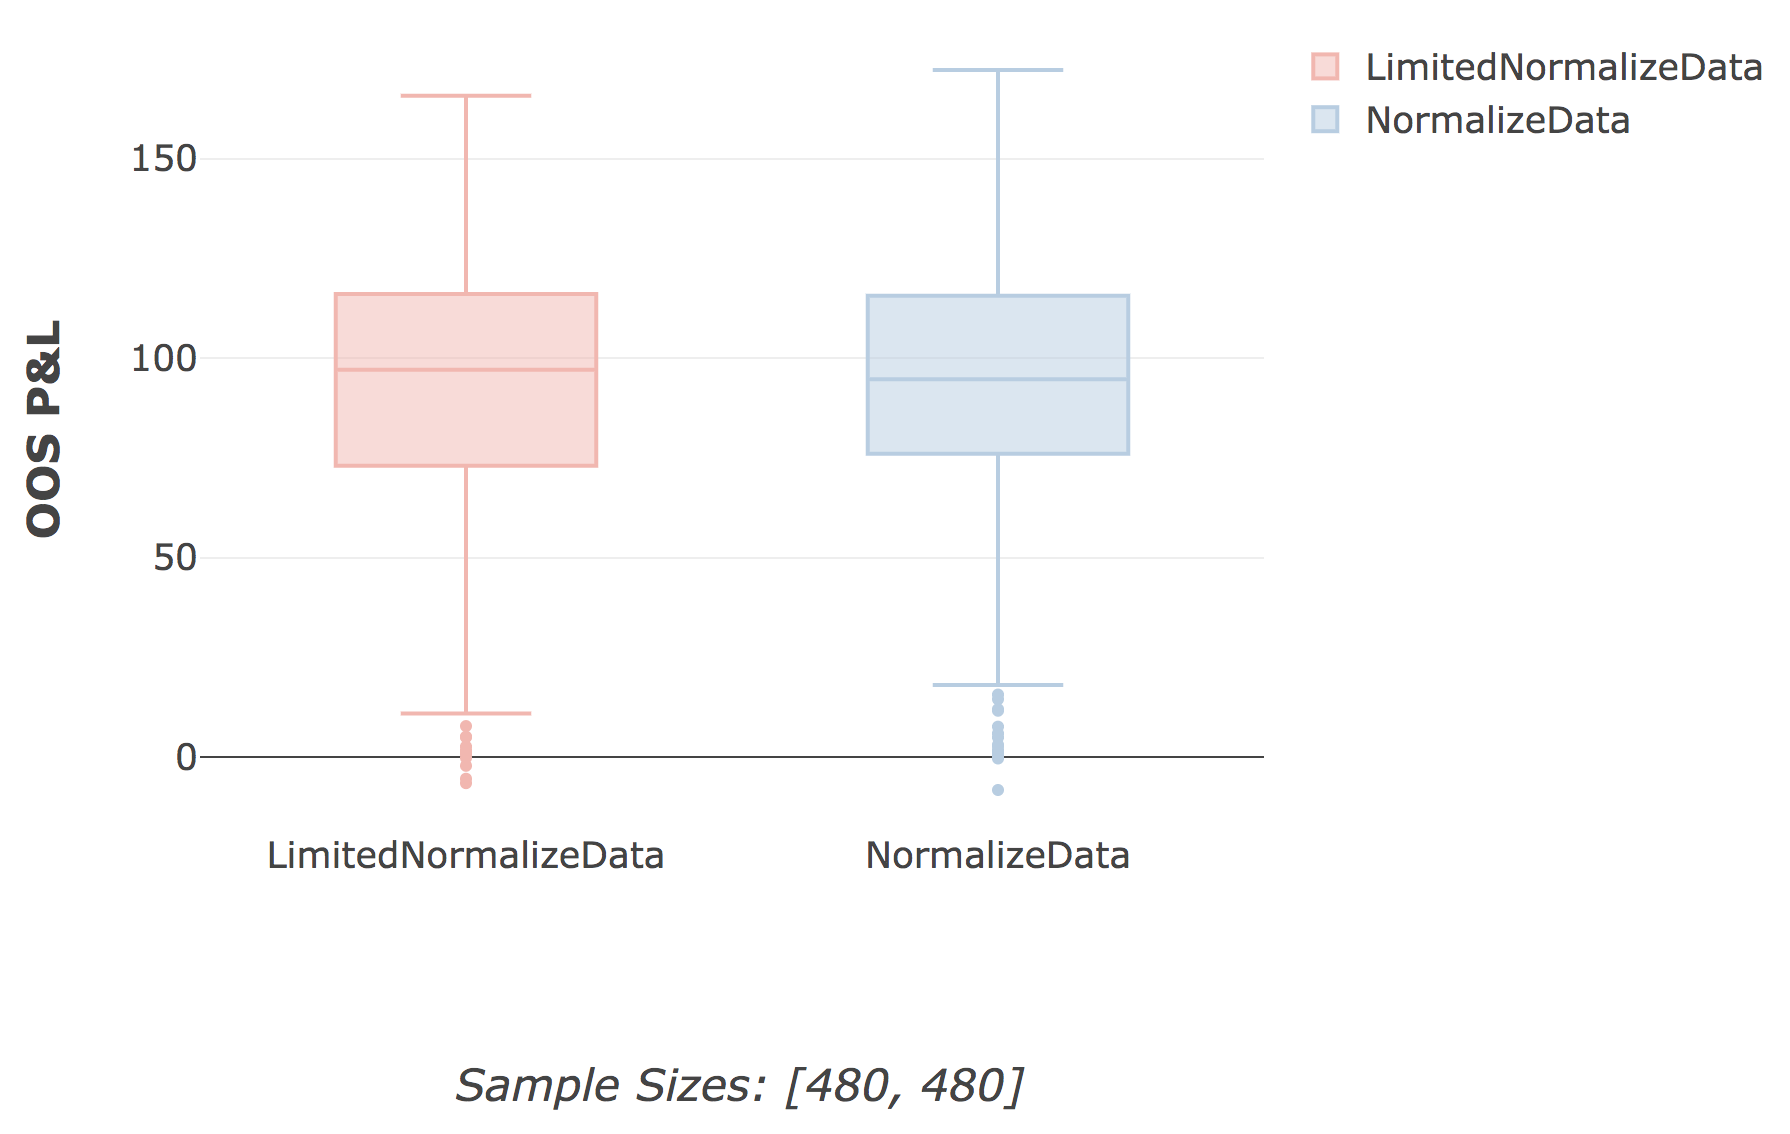
\includegraphics[scale=0.4]{images/results/8_6_complexity/oos_scaling.png}
		\caption[OOS P\&L by Scaling (Synthetic Data)]{Dataset Synthetic6  (\ref{dataset_synthetic6}), Configuration 3 (\ref{config3}) \& Configuration 4 (\ref{config4})
				\newline The figure here shows the impact of the limited scaling technique (as described in Section \ref{data_scaling}) in comparison to the non-limited version. There was a minor detrimental effect as a result of OOS no longer falling within the defined bounds for the scaling used, though the use of a Linear output layer was shown to assist in reducing the impact of this effect, seen in Figure \ref{figure-actual_mse_output}. The implementation of this is not a choice when interested in simulating a real world implementation, and with real assets which have changing variance over time it is expected the impact is actually more significant }
		\label{figure-synth_pl_scaling}
	\end{figure}


	
	\subsubsection{SAE Reproduction}

	The ability of an SAE to reproduce data to a smaller encoding is directly related to the variability and complexity of the underlying data, and the extent to which it can be reduced to fundamental underlying features. The impact of data complexity and variance, as well as the different nature of encodings learnt is discussed fully in Section \ref{results_oos_pl} for actual data, and Section \ref{results_synth} for synthetic data. What we discuss here is how learning optimizations can affect the traversal of the complex solution space. \newline
	
	We found that L1 Regularization (implemented as per Section \ref{imp_regularization}) emphasised the different nature of features learnt at different encoding sizes, as discussed in Section \ref{results_oos_pl}. Smaller encoding sizes, which are generalizing by nature, benefit from the regularization. For larger encoding sizes, the regularization simply lowers model fidelity. These performance impacts can be seen in Figure \ref{figure-mse_reg} at both the aggregate and encoding size level. Figure \ref{figure-results_mse_denoising} shows that denoising optimizations (implemented as per Section \ref{imp_denoising}) had detrimental effects, highlighting the lack of benefits in adding noise to an already noisy feature space. Figure \ref{figure-mse_lr} shows the effects of learning rate schedules (implemented as per Section \ref{imp_learning_rate_schedule}), with increased performances shown for different configurations.
	
	\begin{figure}[H]
	\centering
	\textbf{SAE MSE by L1 Regularization}
	\begin{subfigure}{.99\textwidth}
		\centering 
		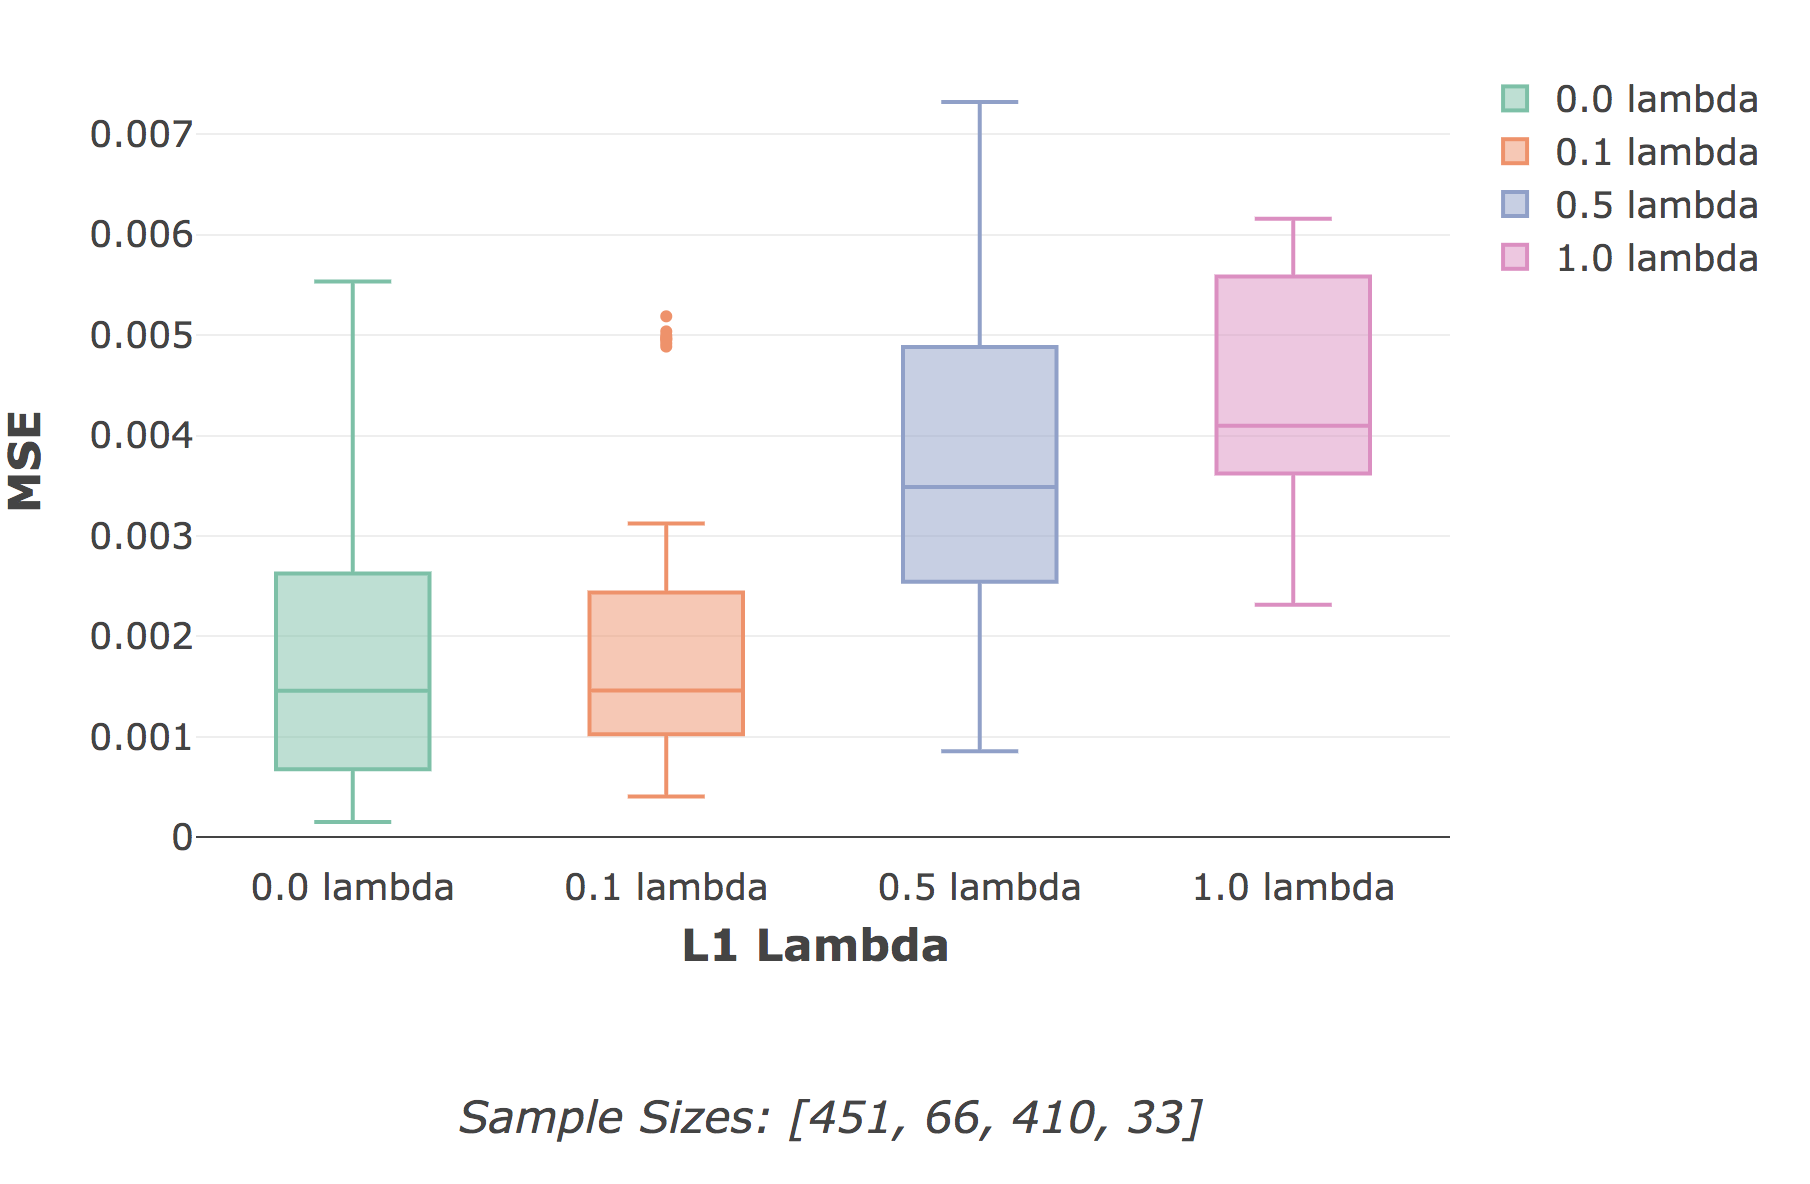
\includegraphics[scale=0.4]{images/results/8_6_complexity/actual_mse_reg.png}
		\caption{\textbf{All Encodings} 
			\newline }
		\label{figure-actual_mse_reg}
	\end{subfigure}
	\begin{subfigure}{.99\textwidth}
		\centering 
		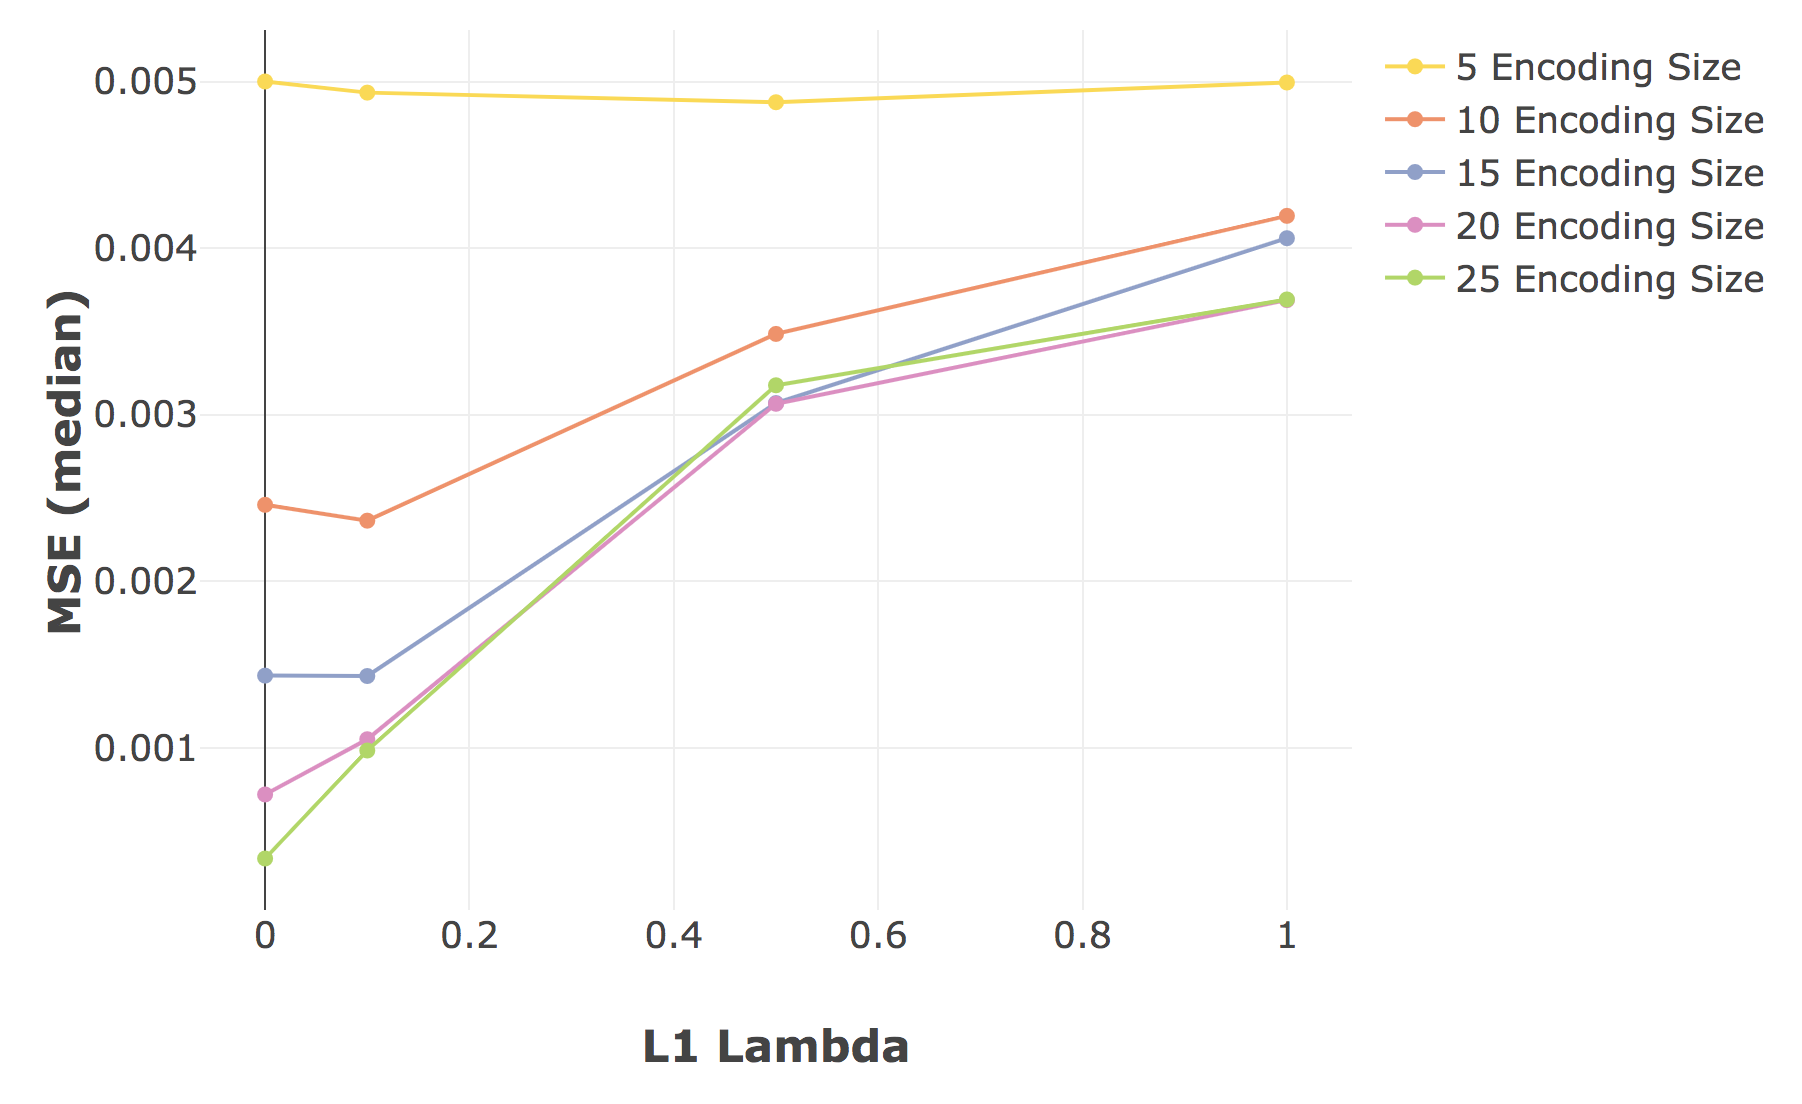
\includegraphics[scale=0.4]{images/results/8_6_complexity/actual_sae_mse_by_encoding.png}
		\caption{\textbf{Split by Encoding Size} 
			\newline }
		\label{figure-actual_sae_mse_by_encoding}
	\end{subfigure}
	\caption[SAE MSE by L1 Regularization]
	{Dataset: Actual10 dataset (\ref{dataset_actual10}), Configuration 12 (\ref{config12})
		\newline Figure (a) shows the aggregate performance of SAE networks at different degrees of regularization, with performance decreasing as regularization increases. Figure (b), grouping by encoding size, provides a better understanding. As per the results in Section \ref{results_oos_pl}, encodings of 5 are learning highly generalisable features, and so benefit from regularization with their best performance at $\lambda = 0.5$. Encodings of 10 have their best performance at $\lambda = 0.1$, learning less generalisable features. Higher encoding levels are operating in a different solution space, and do not benefit from the regularization.
	}
	\label{figure-mse_reg}
	\end{figure}

	\begin{figure}[H]
	\centering
	\textbf{SAE MSE by Denoising Variance}
	\begin{subfigure}{.99\textwidth}
		\centering 
		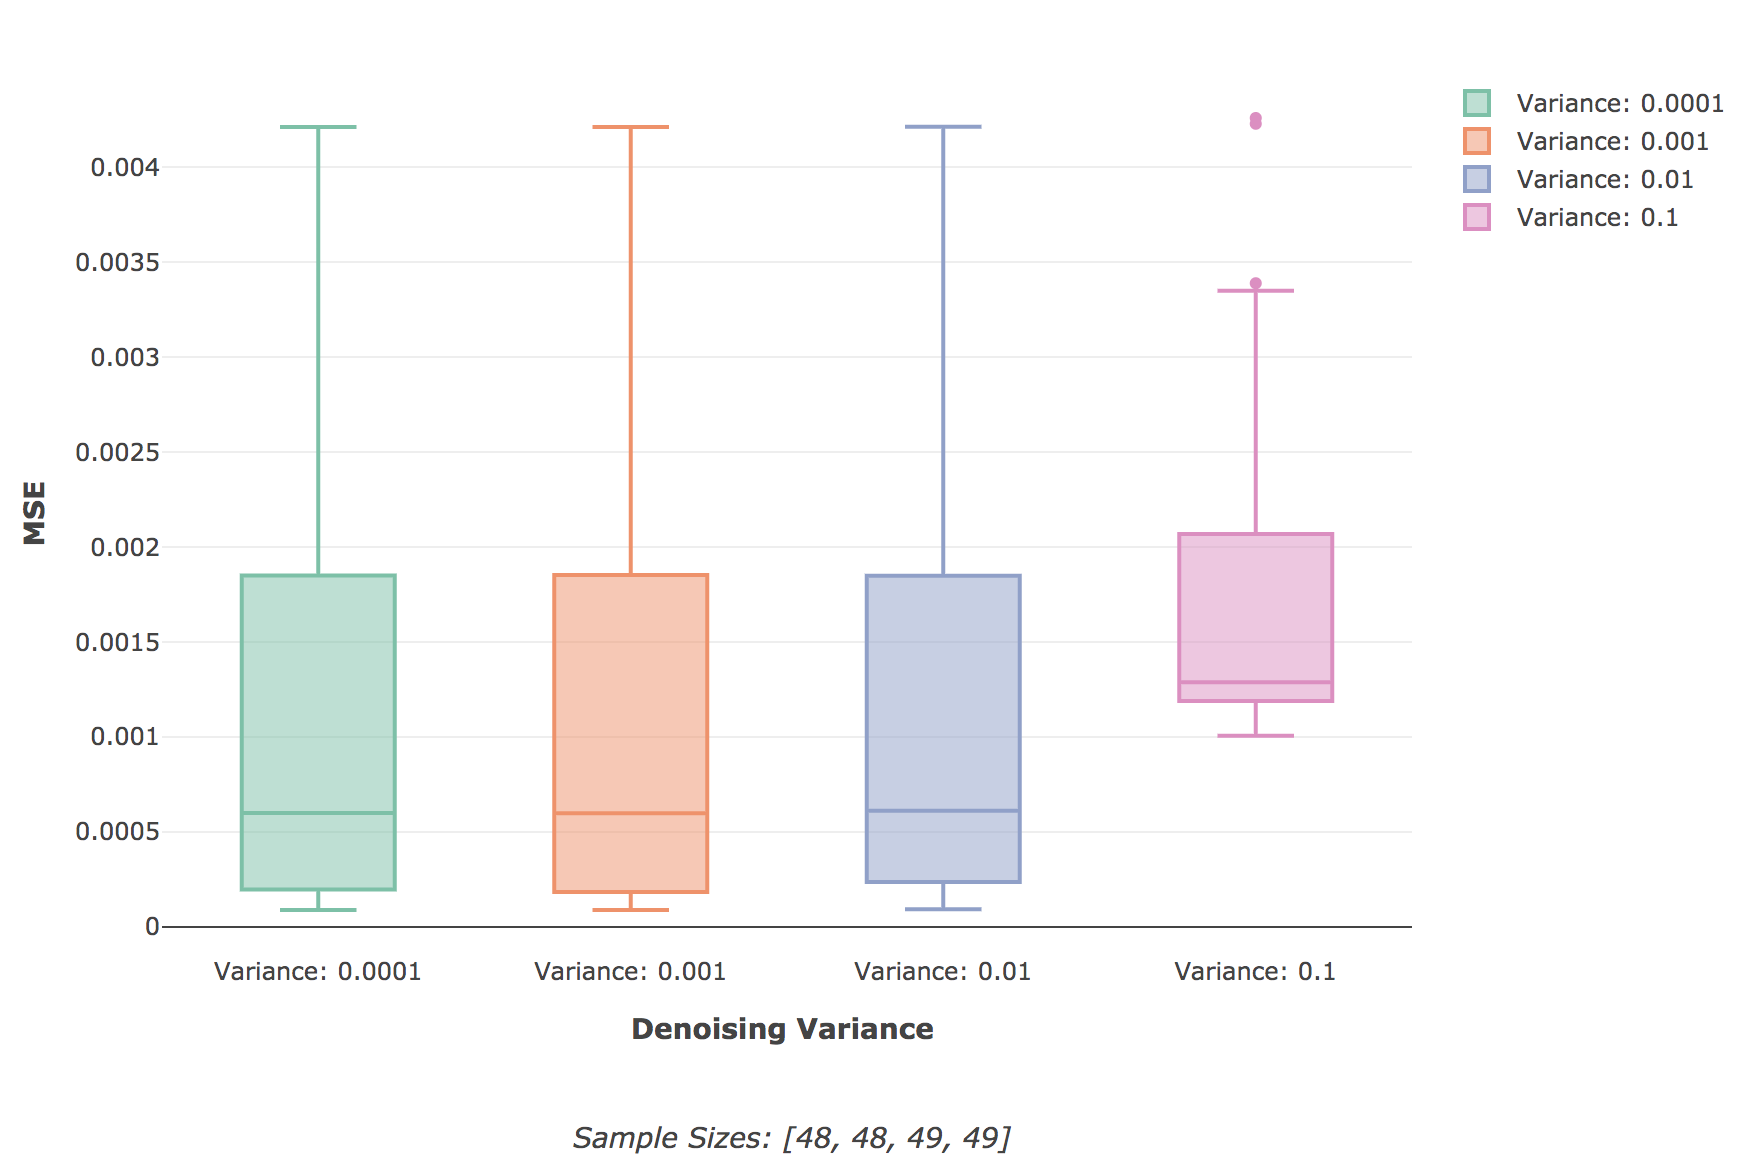
\includegraphics[scale=0.305 ]{images/results/8_6_complexity/actual_mse_gaussian.png}
		\caption{\textbf{Gaussian Denoising} 
			\newline }
		\label{figure-actual_mse_gaussian}
	\end{subfigure}%
	\caption[SAE MSE by Denoising Variance]
	{Dataset: Scaling 10 (\ref{dataset_scaling10}) , Configuration 14 (\ref{config14}) \& Configuration 15 (\ref{config15})
		\newline This figure shows the effects Gaussian denoising had on SAE MSE scores, with scores worsening as the denoising increases. This once again reflects the differences between IID datasets with a model that is likely to overfit in comparison to financial time series data, which already have a significant amount of noise present.}
	\label{figure-results_mse_denoising}
	\end{figure}

	
	\begin{figure}[H]
		\centering
		\textbf{SAE MSE by Learning Rate Schedule Ranges}
		\begin{subfigure}{.5\textwidth}
			\centering 
			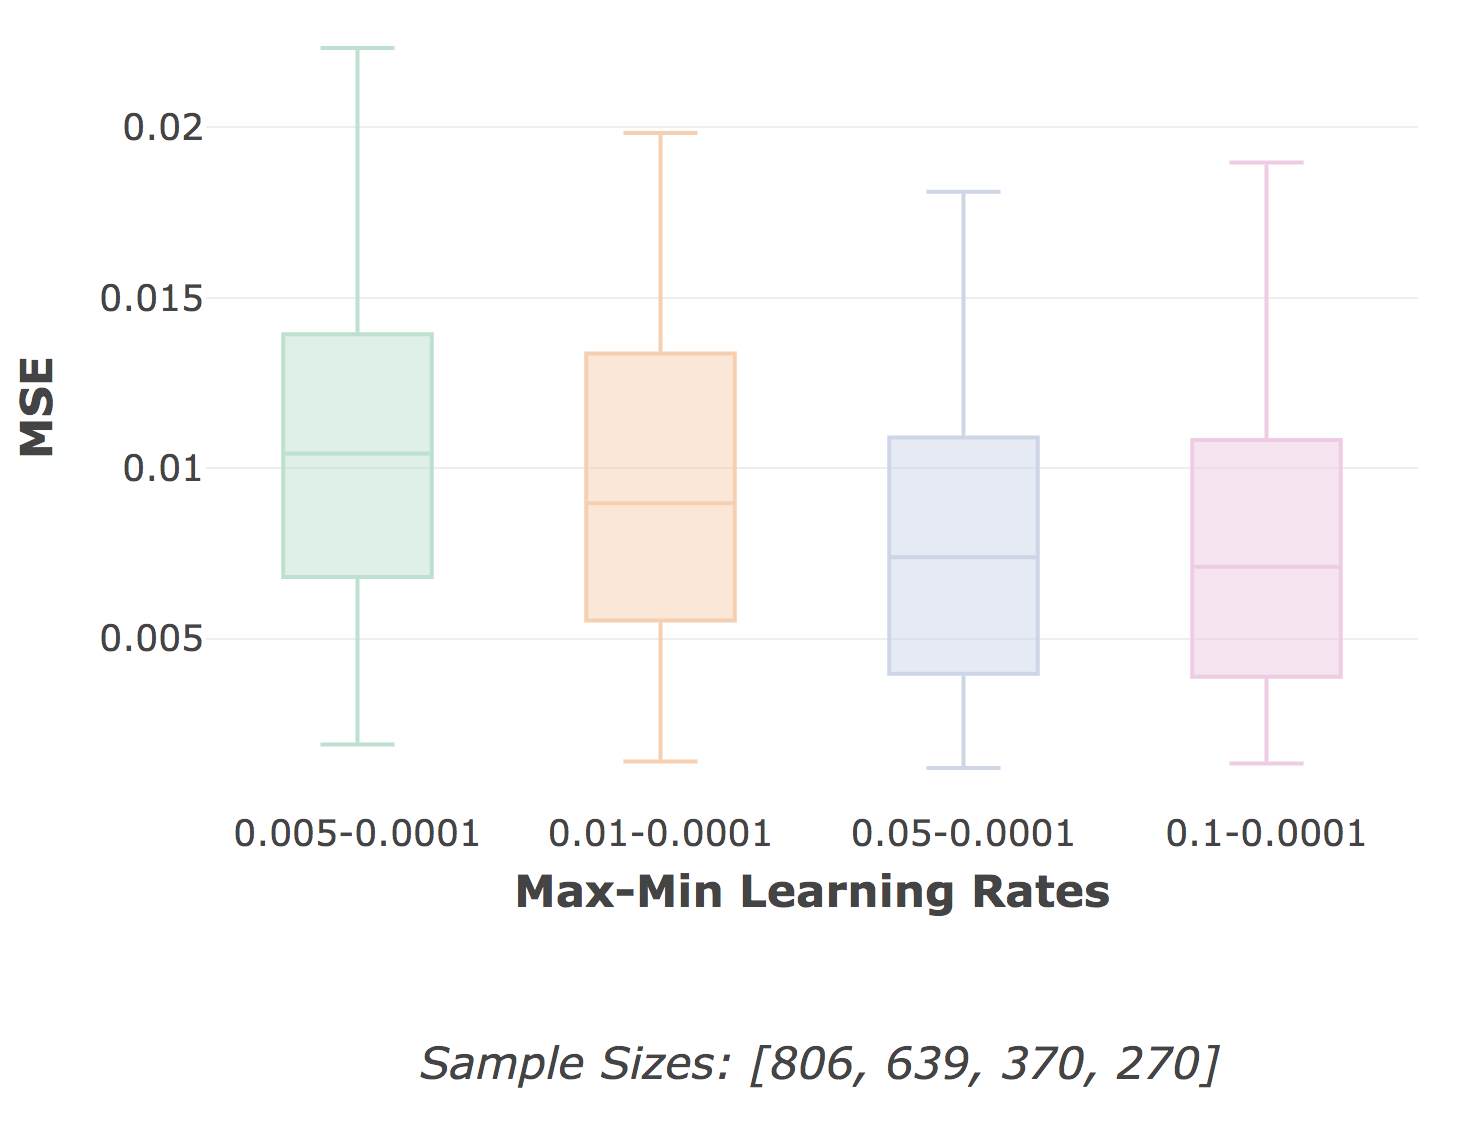
\includegraphics[scale=0.3]{images/results/8_6_complexity/synth_mse_minmax_lr.png}
			\caption{\textbf{Synthetic Data} 
				\newline }
			\label{figure-synth_mse_minmax_lr}
		\end{subfigure}%
		\begin{subfigure}{.5\textwidth}
			\centering 
			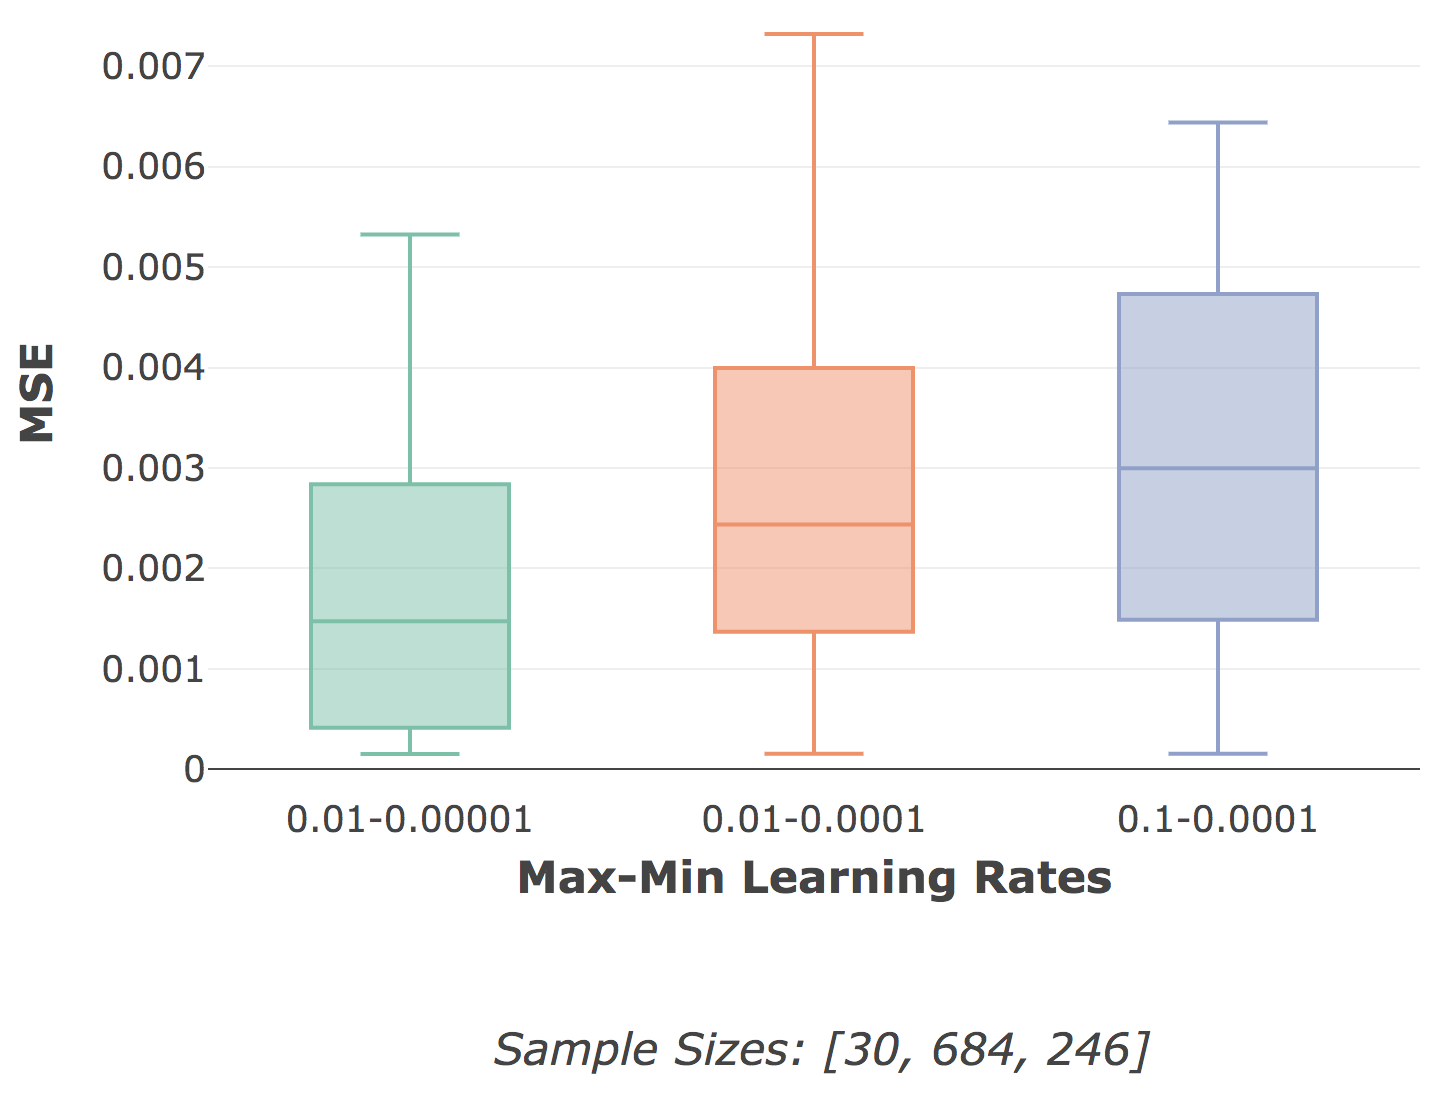
\includegraphics[scale=0.3]{images/results/8_6_complexity/actual_mse_minmax_lr.png}
			\caption{\textbf{Actual Data} 
				\newline }
			\label{figure-actual_mse_minmax_lr}
		\end{subfigure}
		\caption[SAE MSE by Learning Rate Schedule Ranges]
		{Dataset: Synthetic10 (\ref{dataset_synthetic10}), Actual10 (\ref{dataset_actual10}), Configuration 7 (\ref{config7}) \& Configuration 12 (\ref{config12})
			\newline It is interesting to note that the effects of learning rate schedules were so different for Synthetic and Actual data, with networks for Synthetic data favouring learning rate ranges with a higher upper bound, and Actual data networks trending in favour of lower upper bound ranges. The synthetic data is structurally less complex, as discussed in Sections \ref{results_gbm_data} and \ref{results_data_hist}, and so the larger learning rates allowed for quicker optimisation. Conversely, SAE networks for actual data benefit from a more careful exploration of the solution space. The different epoch lengths had a marginal effect, as seen in Appendix \ref{results_appendix_finance_data}.}
		\label{figure-mse_lr}
	\end{figure}

	

	

	
	
	
	
	
	
	
	
	\newpage
	\subsubsection{FFN Prediction}
	
	As we discussed in Section \ref{results_data_hist}, the effects of supervised training on the IS dataset with SGD had limited benefits for OOS performance, and ultimately may be approximating the equivalent of pretraining weight initialization rather than an effective structural learning. The best performing networks were those which were able to quickly adapt to new solution spaces, rather than those which had trained effectively to old ones. Naturally then, the numerous SGD optimizations employed had very little effect on the OOS performance. That said, the effects they have on IS performance do give some insights into the nature of financial data being considered, and do suggest that implementing learning optimizations in the OGD phase could be beneficial. \newline
		
	Figure \ref{figure-actual_pl_lr_epochs} shows the effects of learning rate schedules (implemented as per Section \ref{imp_learning_rate_schedule}), with notable impact across different epoch lengths. Figure \ref{figure-results-reg} shows the impact of L1 regularization (implemented as per Section \ref{imp_regularization}), with results showing only a minor potential improvement and highlighting the unstable dynamics of financial time series. Lastly, Figure \ref{figure-results_mse_denoising} shows that input Dropout (implemented as per Section \ref{imp_dropout}) was ineffective in prompting the network to learn interactive relations between assets.
		
		
	\begin{figure}[H]
		\centering
		\textbf{Effects of Epoch Cycle Lengths on P\&L}
		\begin{subfigure}{.46\textwidth}
			\centering 
			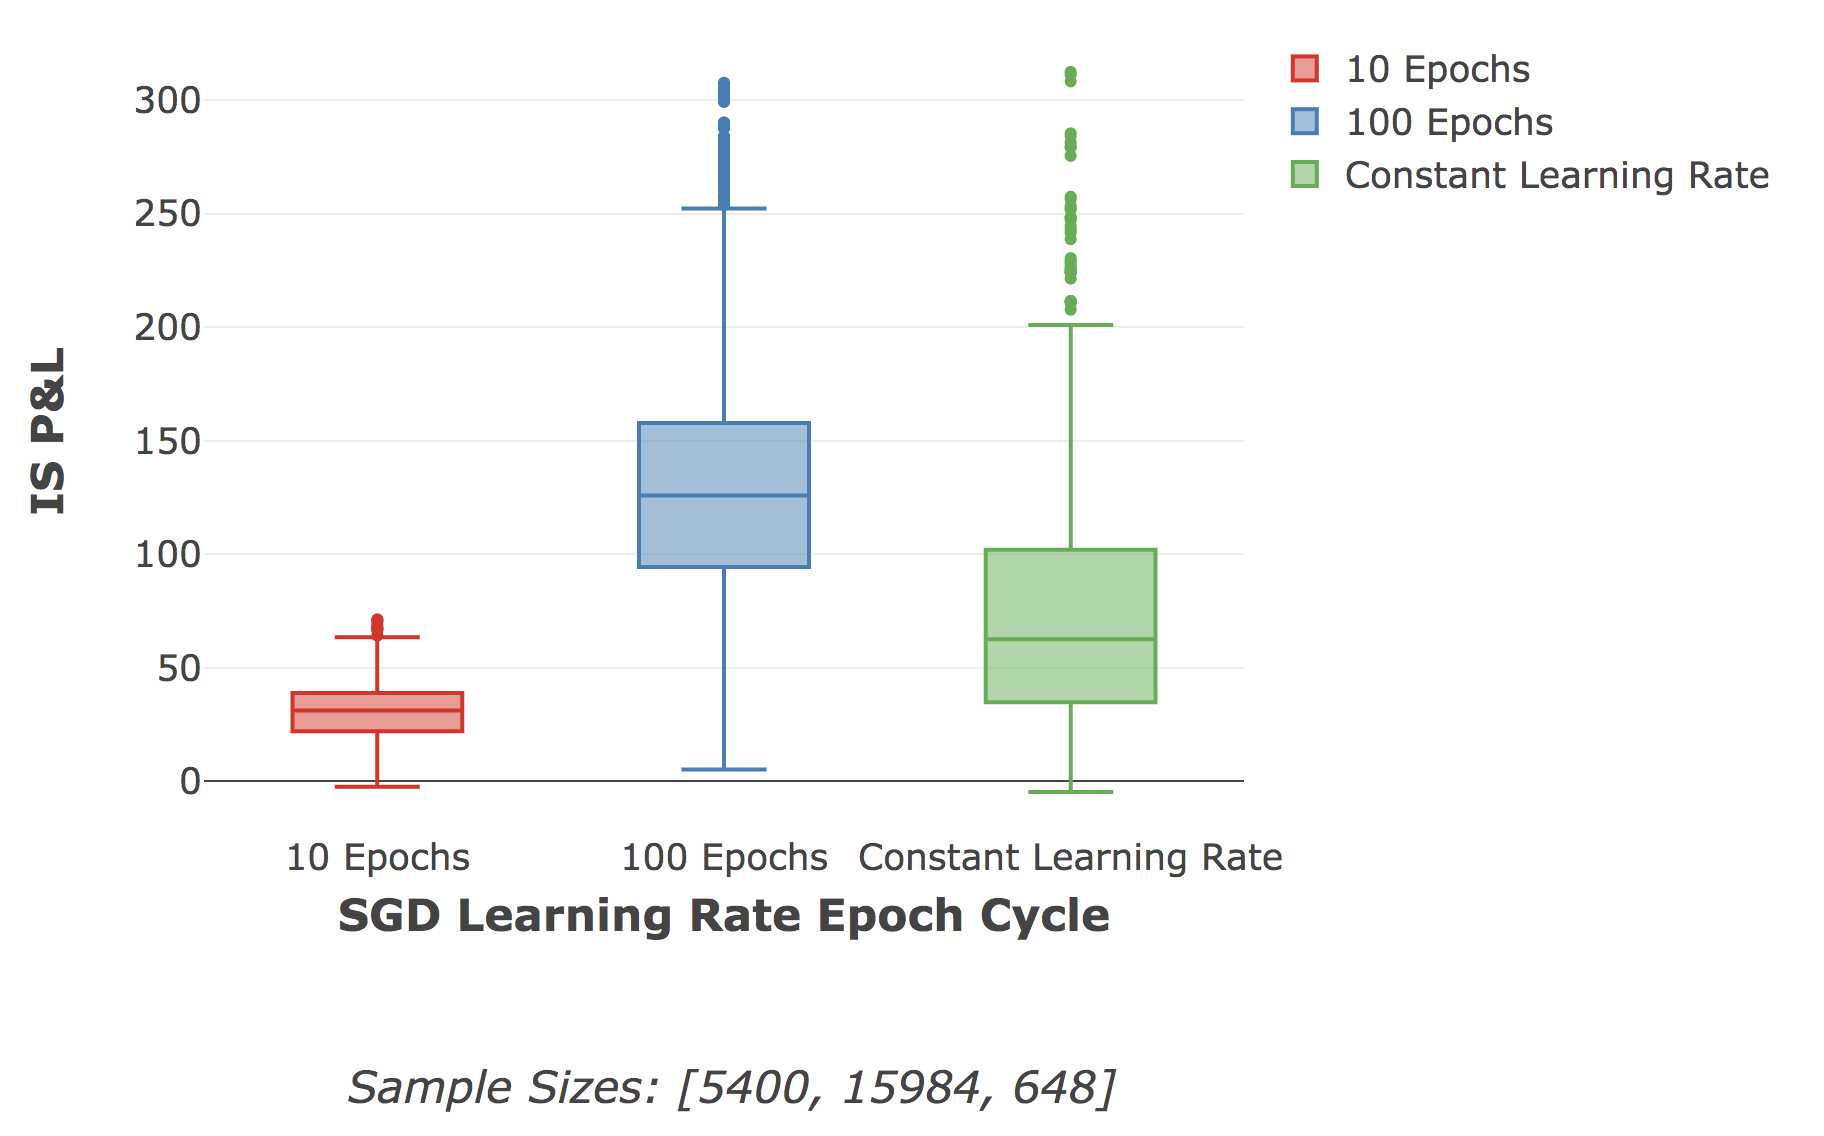
\includegraphics[scale=0.33]{images/results/8_6_complexity/IS_actual_pl_lr_epochs.png}
			\caption{\textbf{IS P\&L} 
				\newline }
			\label{figure-actual_is_pl_lr_epochs}
		\end{subfigure}%
		\begin{subfigure}{.48\textwidth}
			\centering 
			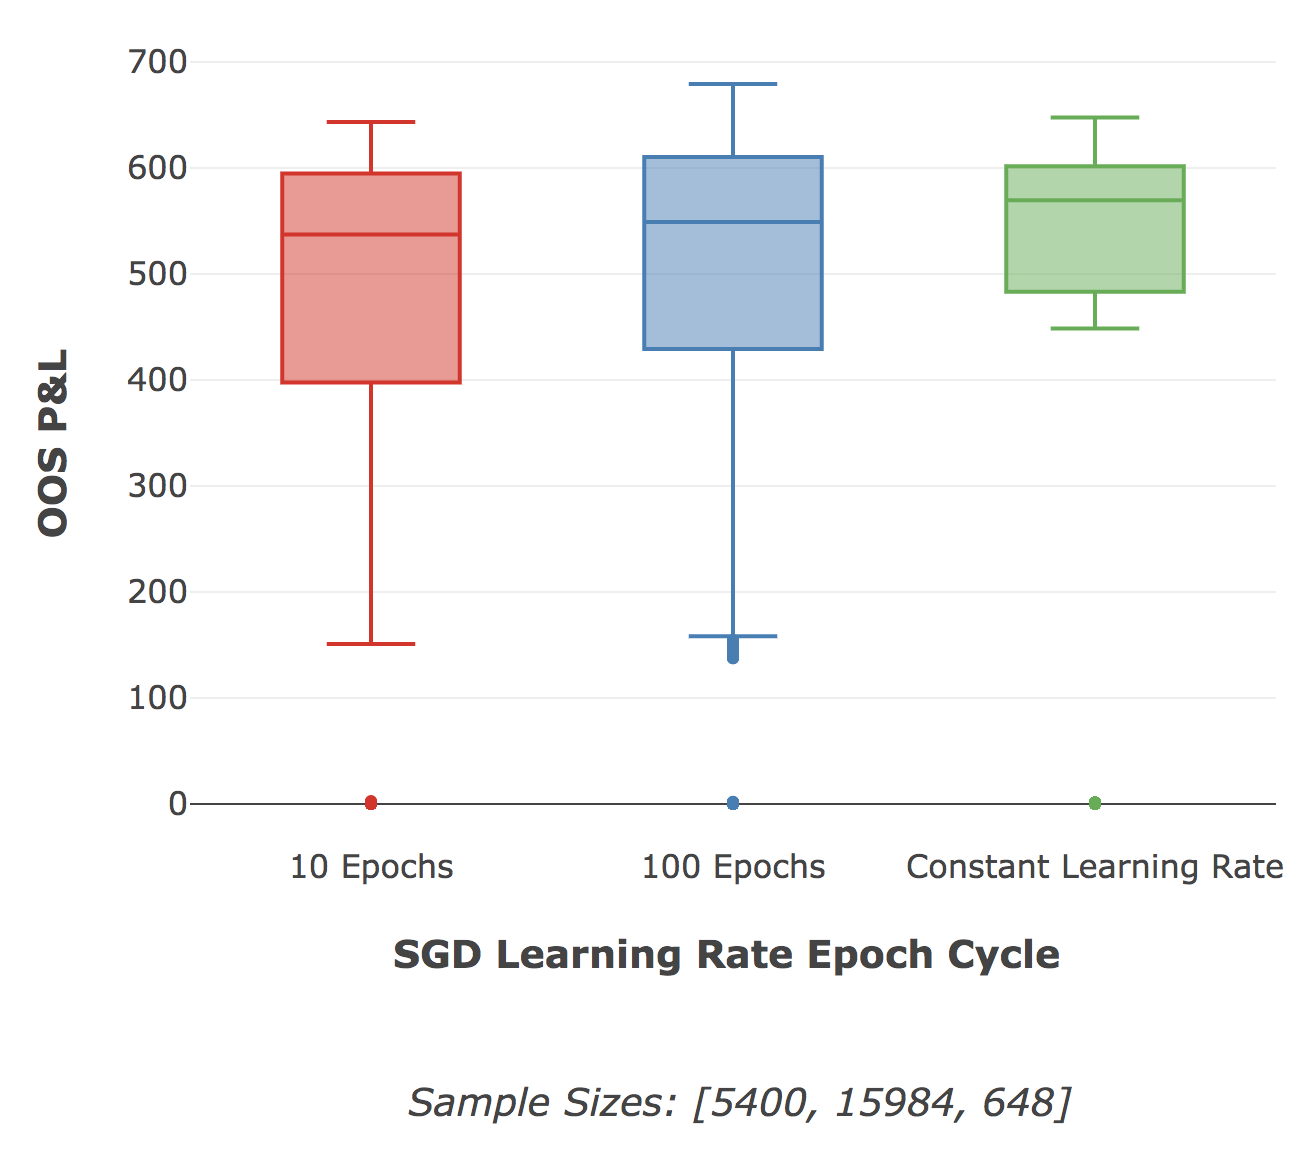
\includegraphics[scale=0.32]{images/results/8_6_complexity/OOS_actual_pl_lr_epochs.png}
			\caption{\textbf{OOS P\&L} 
				\newline }
			\label{figure-actual_oos_pl_lr_epochs}
		\end{subfigure}
		\caption[Effects of Epoch Cycle Lengths on P\&L]
		{Dataset: Actual10 dataset (\ref{dataset_actual10}), Configuration 13 (\ref{config13})
		\newline Figure (a) shows significant differences in the P\&L compared across different learning rate epochs, with 100 offering notable improvement over  a constant learning rate. The 10 epoch cycles were used for configurations which only ran for 10 epochs, and so the performance may just be indicative of the amount of training. As expected, the performance increase IS doesn't have significant impacts on the OOS performance seen in Figure (b), but it does given an indication that a more careful exploration of the complex solution space would be beneficial where possible.
		\newline\newline
		The learning rate ranges themselves were set to the best values seen for the data in the SAE training, and small variations did not result in notable changes. These can be seen in Appendix \ref{results_appendix_finance_data}.}
		\label{figure-actual_pl_lr_epochs}
	\end{figure}
	
	\begin{figure}[H]
		\centering
		\textbf{Effects of L1 Regularization on P\&L}
		\begin{subfigure}{.5\textwidth}
			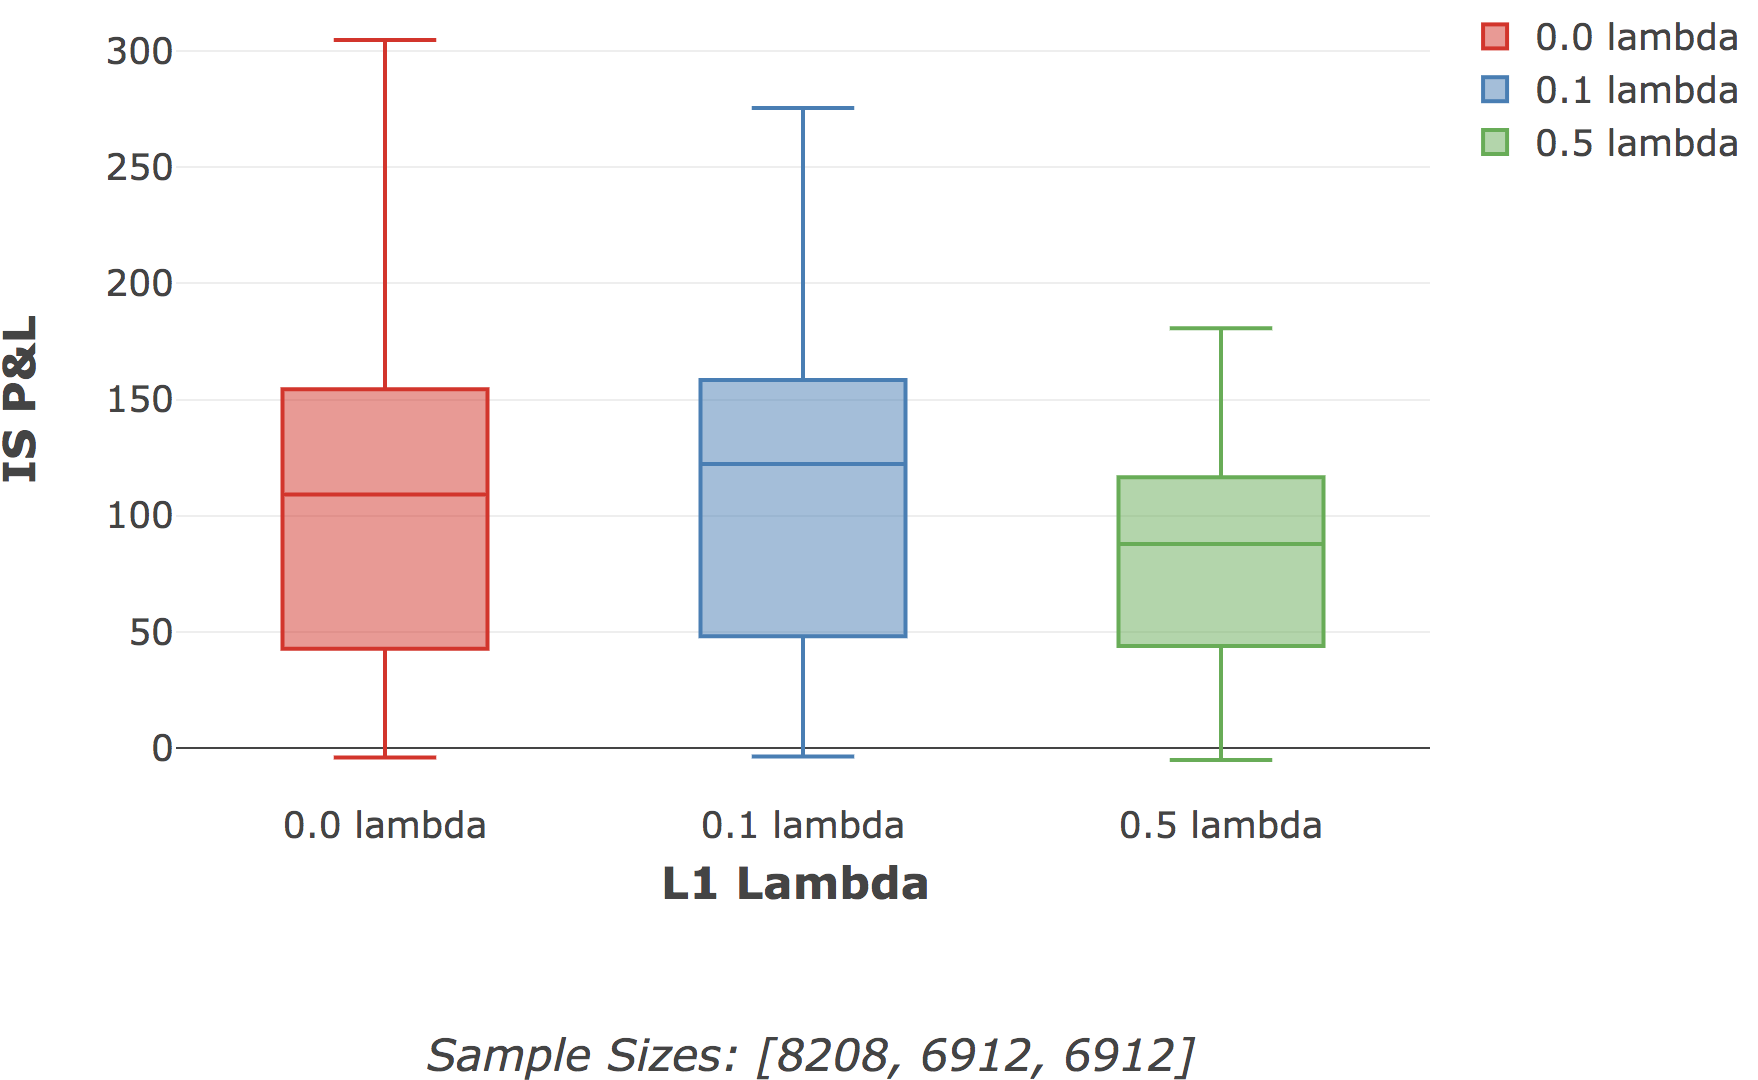
\includegraphics[scale=0.305]{images/results/8_6_complexity/is_actual_pl_reg.png}
			\caption{\textbf{IS P\&L} }
			\label{figure-is_actual_pl_reg}
		\end{subfigure}%
		\begin{subfigure}{.5\textwidth}
			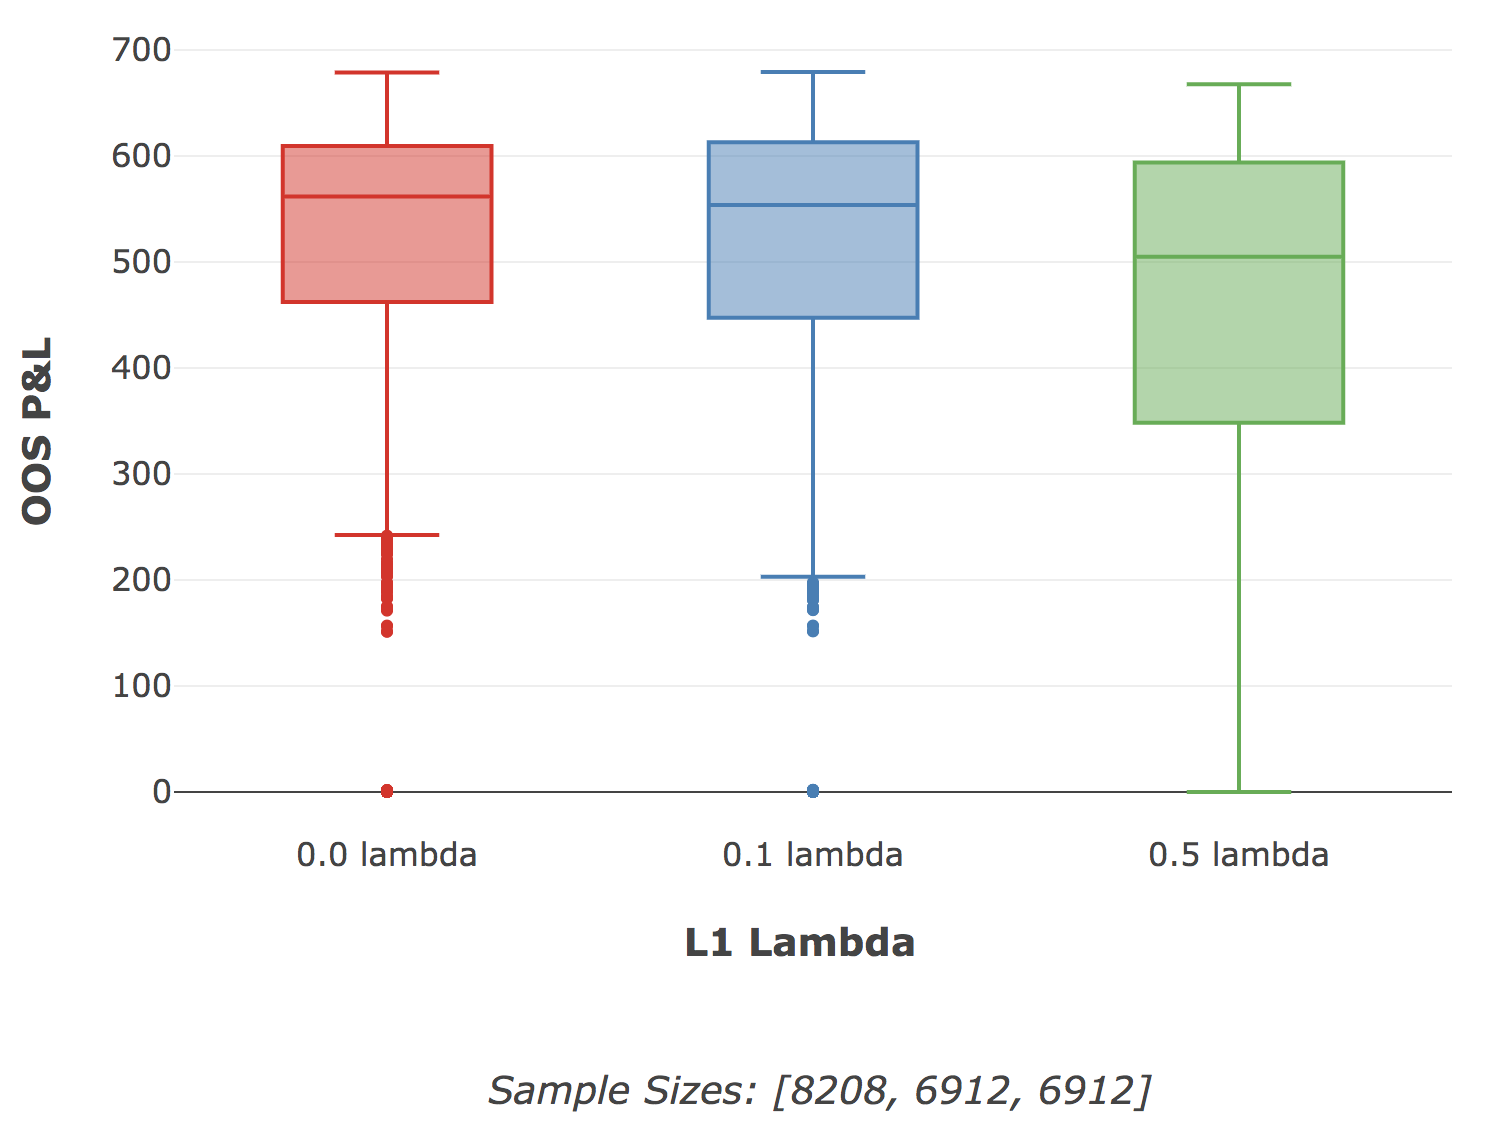
\includegraphics[scale=0.3]{images/results/8_6_complexity/oos_actual_pl_reg.png}
			\caption{\textbf{OOS P\&L} }
			\label{figure-oos_actual_pl_reg}
		\end{subfigure}
		\caption[Effects of L1 Regularization on P\&L]
		{Dataset: Actual10 dataset (\ref{dataset_actual10}),  Configuration 13 (\ref{config13})
			\newline L1 Regularization in Figure (a) shows mostly poorer aggregate IS performance with lower P\&L and with only detrimental follow through to the OOS performance, as seen in Figure (b). This highlights that even when a model generalises for IS data, the changing dynamics of financial time series means that it may not be generalising well for OOS data. L1 regularization is expected to work well in instances of IID data, but for time series financial data, where the model is not overfitting, it is just affecting model fidelity. This effect is amplified both IS and OOS when $\lambda = 0.5$.}
		\label{figure-results-reg}
	\end{figure}
	
	\begin{figure}[H]
		\centering
		\textbf{Effects of Dropout on P\&L}
				\begin{subfigure}{.5\textwidth}
			\centering 
			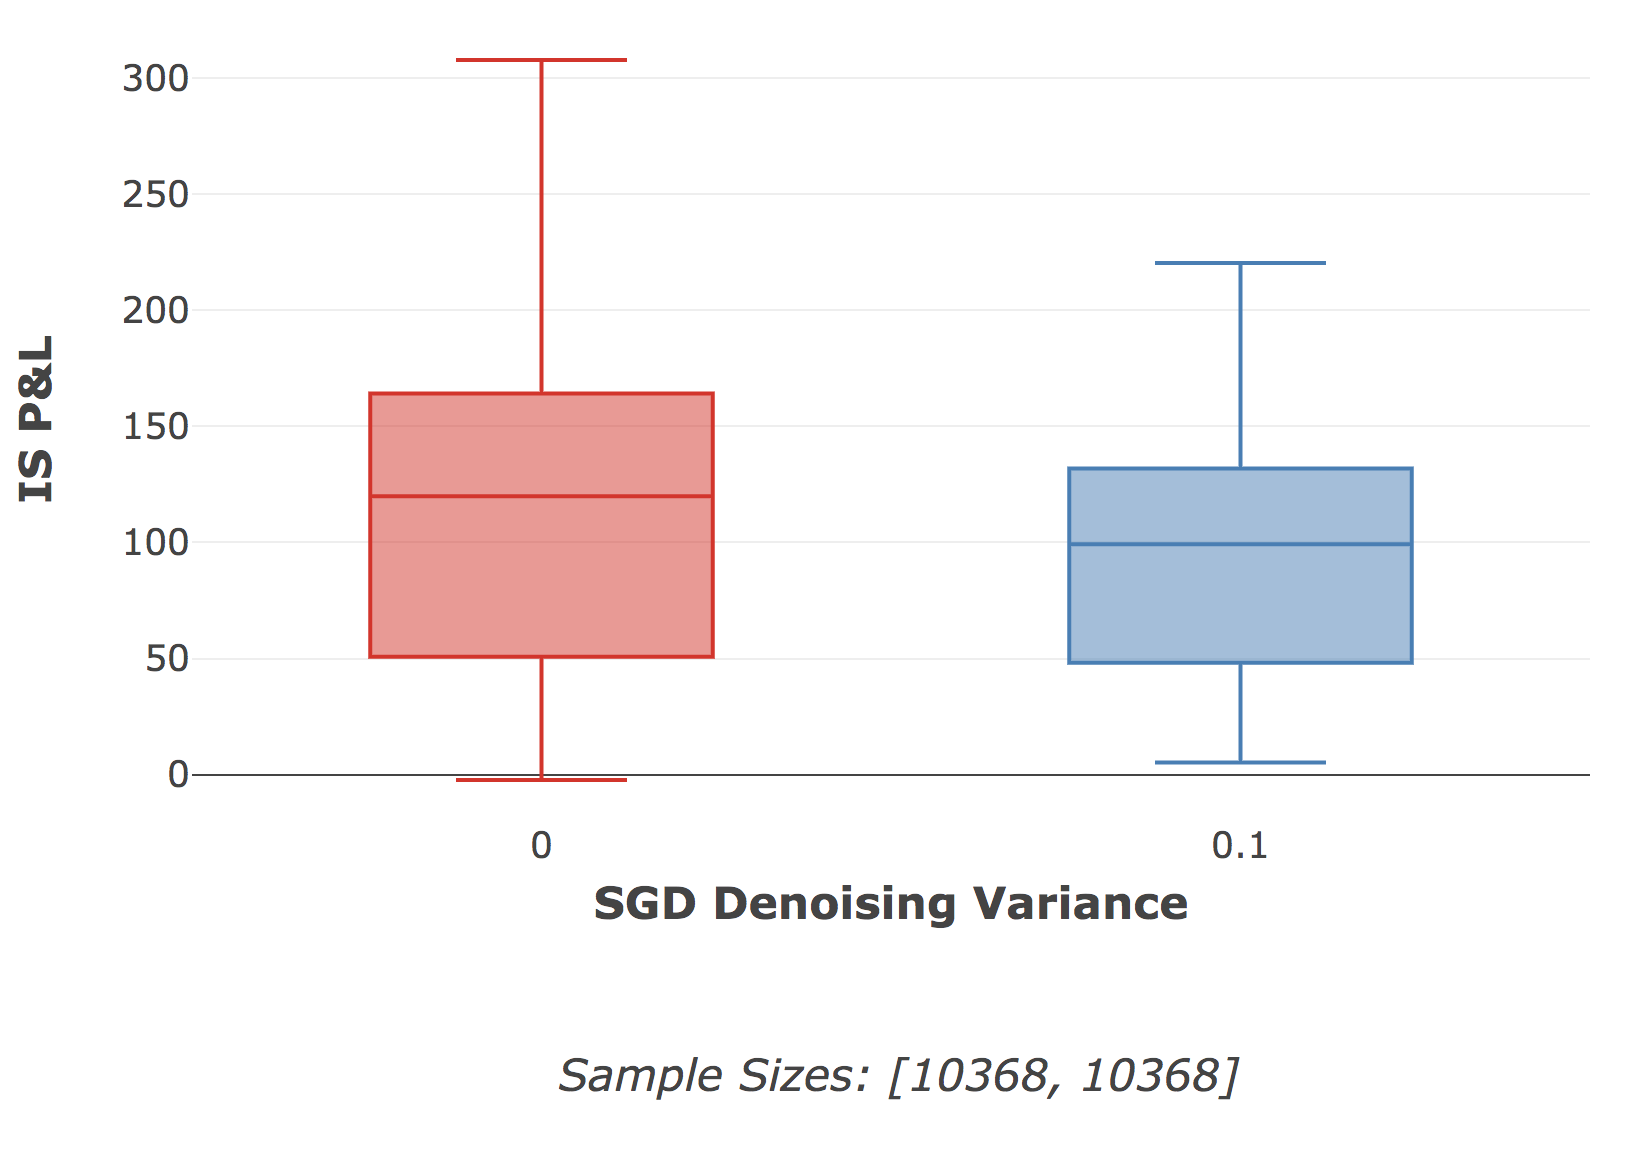
\includegraphics[scale=0.305]{images/results/8_6_complexity/is_actual_pl_masking.png}
			\caption{\textbf{IS P\&L} }
			\label{figure-is_actual_pl_masking}
		\end{subfigure}%
		\begin{subfigure}{.5\textwidth}
			\centering 
			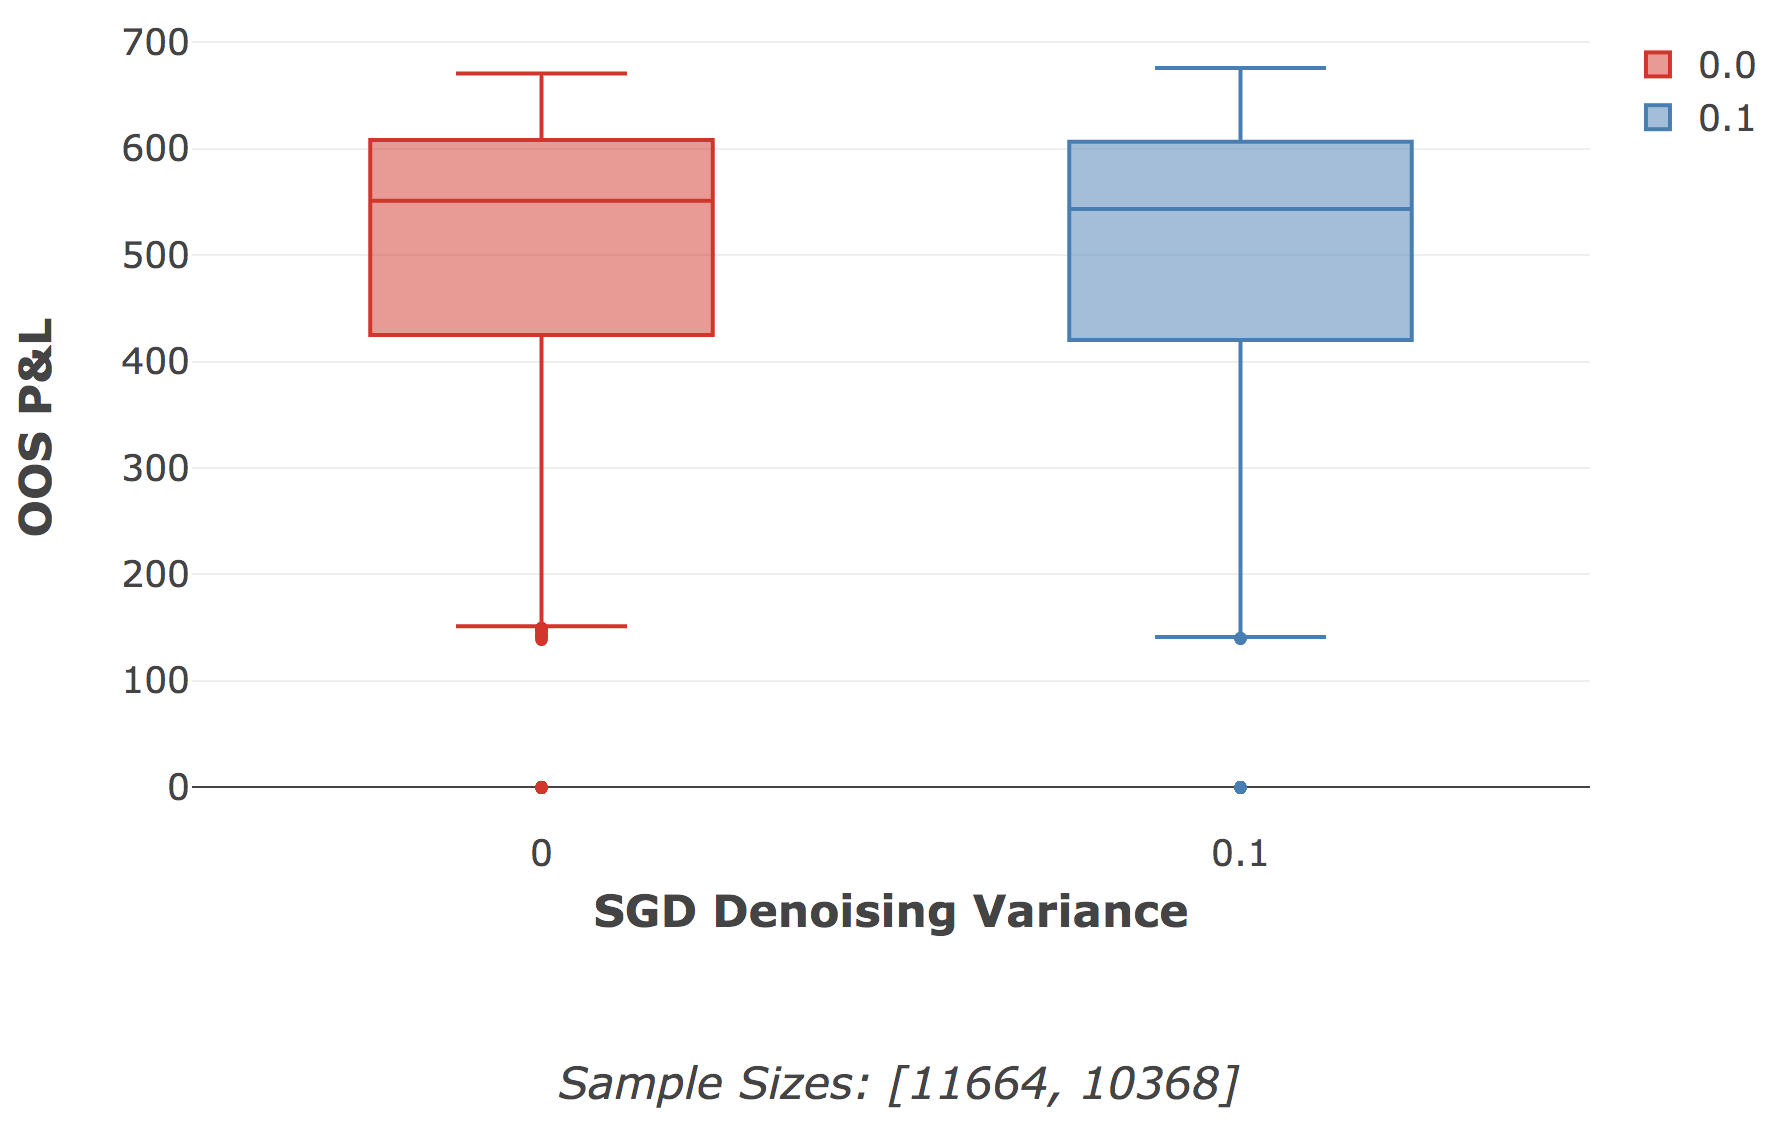
\includegraphics[scale=0.3]{images/results/8_6_complexity/oos_actual_pl_masking.png}
			\caption{\textbf{OOS P\&L} }
			\label{figure-oos_actual_pl_masking}
		\end{subfigure}
		\caption[Effects of Dropout on P\&L]{Dataset: Actual10 dataset (\ref{dataset_actual10}), Configuration 13 (\ref{config13})
			\newline Input Dropout was tested on the predictive FFN networks in the hope that it might encourage the network to increase learning about the relationships between assets. The results for 10\% variation had a detrimental impact on IS performance, though with little impact on OOS P\&L.}
		\label{figure-actual_pl_masking}
	\end{figure}
		
	\newpage

	\subsection{Network Structure}\label{results_network}
	
	\subsubsection{Effects of Network Size}
	
	We found that increasing network layers or layer sizes usually led to better performance in both SAE and FFN networks. The exception was for some of the networks with smaller sized layers (i.e. 120 nodes for SAE networks), which struggled with training. The effects can be seen for both SAE MSE and FFN P\&L in Figure \ref{figure-network_size} below. The trends for both actual and synthetic data were largely the same, and so only actual data has been considered here.
	
	It was interesting to see that the typically accepted SAE network structure, where layers decrease in size between the input layer and the encoding layer, resulted in worse performance (as compared to the same number of layers with a constant number of nodes). As detailed in Section \ref{results_init}, the RBM based greedy layerwise pre-training proved to be ineffective, and so variance based weight initialization with SGD training on the entire network was used instead. It was seen that for SGD training, larger layers at all stages improved performance. It is possible that a greedy layerwise training using variance based weight initialization may have shown increased performance in the decreasing layer size structure. The box plots showing these trends can be seen for actual and synthetic data in Appendix \ref{results_network_appendix}.
	
	\subsubsection{Effects of Activation Functions}\label{results_activations_scaling}
	
	We test a range of activation functions (Linear, ReLU and Sigmoid) (as described in Section \ref{imp_activation_functions}) on actual data for SAE networks to determine the best configurations going forward. We found that Linear activations are best for the encoding and output layers, and that ReLU activations largely outperform Sigmoid or Linear activations for the hidden layers (Figures \ref{figure-actual_mse_output} and \ref{figure-mse_encoding_activations} below). This makes sense with the non-linear benefit at hidden layers but with less loss of error signal and information at the output and encoding layers. These results were used for subsequent parameter choices.
	
	\subsubsection{Predictive FFN Activations}
	
	Predictive network activation functions were only tested on synthetic data. With the results for the SAE networks available, the risk of increasing PBO from more configurations did not seem necessary. We found that reconstruction of aggregated GBM data was able to be performed quite effectively through linear activations, so long as the network (and encoding layers) were large enough to allow for sufficient transformations. Linear activations were not tested further on actual data, as there is no reason to believe the time series would continue to exhibit the constant drift with non-independent price jumps over time. 
	
	\subsubsection{Sigmoid Activation Functions} 
	
	Due to the poor performance seen in Sigmoid function based SAEs, as well as the poorer results when compared to ReLU activations, Sigmoid functions were largely excluded from further configuration testing.
	
	\subsubsection{Leaky ReLU vs. ReLU}
	
	We found that the Leaky ReLU activations had only minor effects for SAE, which can be seen in Appendix \ref{results_network_appendix}. For the predictive network, the LeakyReLU did offer some more significant improvements (3\% - 10\%) on OOS P\&L for Synthetic data, as seen in Figure \ref{figure-synthetic_pl_leakyrelu}. Subsequently, Leaky ReLU was used as the hidden layer activation of choice for most trials.
	
	\begin{figure}[H]
		\centering
		\textbf{Network Performance by Size}
		\begin{subfigure}{.99\textwidth}
			\centering 
			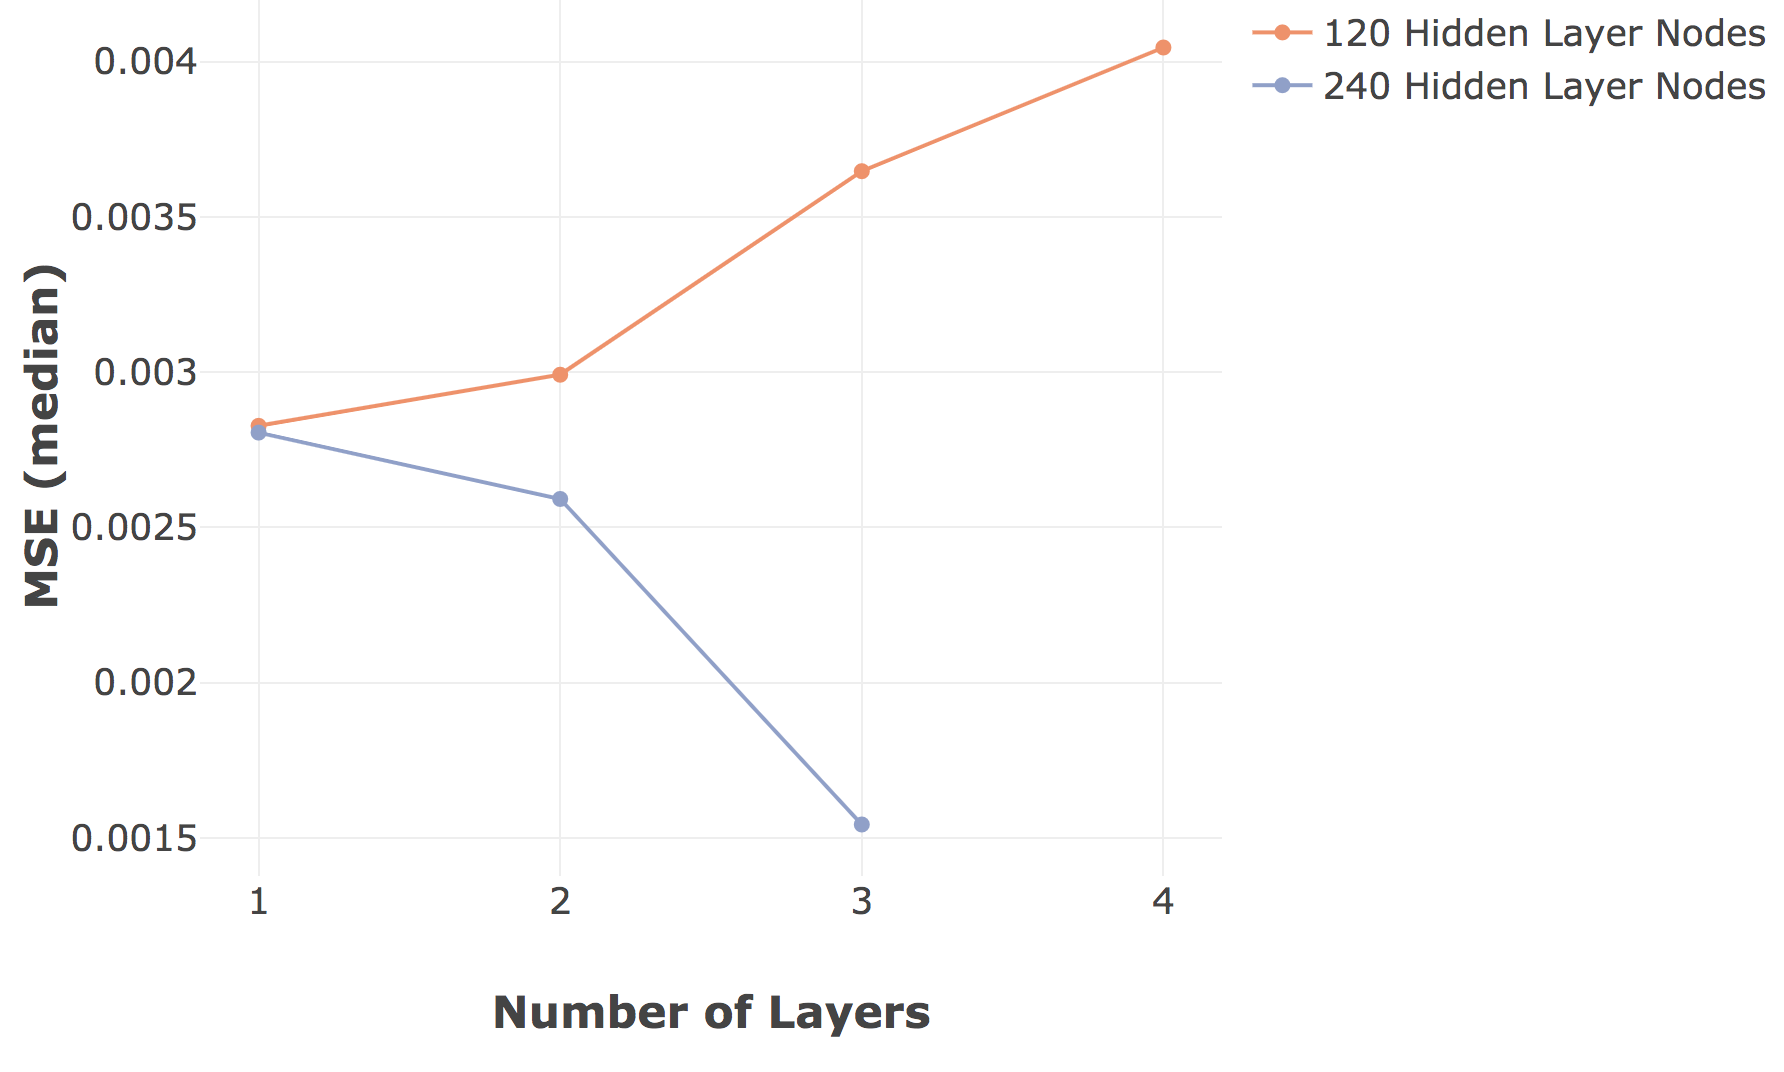
\includegraphics[scale=0.4]{images/results/8_7_network/actual_mse_lines.png}
			\caption{\textbf{SAE MSE Scores} 
				\newline }
			\label{figure-actual_mse_lines}
		\end{subfigure}
		\begin{subfigure}{.99\textwidth}
			\centering 
			\includegraphics[scale=0.4]{images/results/8_7_network/actual_pl_lines.png}
			\caption{\textbf{Predictive P\&L Scores} 
				\newline }
			\label{figure-actual_pl_lines}
		\end{subfigure}
		\caption[Network Performance by Size]
		{Dataset: Actual10 dataset (\ref{dataset_actual10}), Configuration 12 (\ref{config12}) \& Configuration 13 (\ref{config13})
			\newline Figure (a) shows the median MSE by SAE networks achieved with the indicated number of layers and layer nodes. The number of layers here indicate the final SAE structure of $N$ hidden layers, rather than the training structure of $2N + 1$ hidden layers. The networks with 120 node layers struggled with training, and performance decreases as layers increased. This is to be expected if the learning parameters (e.g. SGD  learning rate) are not ideal for the structure, the effects of which are amplified as network sizes increase. This was resolved in the larger 240 node networks which show significant improvement as more layers are added (as one would generally expect, subject to effective SGD).
			\newline Figure (b) shows the median OOS P\&L achieved by predictive networks with the indicated number of layers and layer nodes. The behaviour was as expected here, where network performance usually improves with size. The exception was the four layer network of 60 nodes, where the training parameters were no longer effective in passing signal back (larger layer sizes are less likely to suffer from this, particularly with ReLU activations).
		}
		\label{figure-network_size}
	\end{figure}
	
	\newpage
	\begin{figure}[H]
		\centering
		\textbf{SAE MSE by Activations and Encoding Layer Size}
		\begin{subfigure}{.99\textwidth}
			\centering 
			\includegraphics[scale=0.4]{images/results/8_7_network/actual_mse_encoding.png}
			\caption[MSE by Activations and Encoding Layer Size - Encoding Activations]{\textbf{Encoding Activations} 
				\newline }
			\label{figure-actual_mse_encoding_activations}
		\end{subfigure}
		\begin{subfigure}{.99\textwidth}
			\centering 
			\includegraphics[scale=0.4]{images/results/8_7_network/actual_mse_hidden.png}
			\caption[MSE by Activations and Encoding Layer Size - Hidden Activations]{\textbf{Hidden Activations} 
				\newline }
			\label{figure-actual_mse_hidden_activations}
		\end{subfigure}
		\caption[MSE by Activations and Encoding Layer Size]
		{Dataset: Scaling10 dataset (\ref{dataset_scaling10}), Configuration 2 (\ref{config2})
			\newline Figure (a) shows the best (minimum) MSE scores for different encoding activations at the different encoding layer sizes (with a network input of 30). There was consistent outperformance by Linear activations in the encoding layer, which is expected from literature \citep{Hinton2}, and in line with reducing loss of error signal at critical points. 
			\newline Figure (b) shows the best (minimum) MSE scores for different hidden layer activations at the different encoding layer sizes (with a network input of 30). At larger encoding layers, there was competitive performance from fully linear networks, where they are less pressured to take advantage of non-linear effects. As the size of the encoding layer is reduced, the advantages of non-linear activations become more apparent, with outperformance by ReLU and Sigmoid activations. Sigmoid activations are known to suffer from learning slow down as a result of saturation and so have increased sensitivity to vanishing gradients \citep{Glorot2}. SAE networks are deep by nature, and so it is not surprising that the Sigmoid activations resulted in worse performance over the same training period when compared to ReLU activations. \newline}
		\label{figure-mse_encoding_activations}
	\end{figure}
	
	\begin{figure}[H]
		\begin{center}
			\centering
			\textbf{SAE MSE by Output Activations}
			\includegraphics[scale=0.4]{images/results/8_7_network/actual_mse_output.png}
			\caption[MSE by Output Activations]
			{Dataset: Scaling10 dataset (\ref{dataset_scaling10}), Configuration 1 (\ref{config1})
				\newline This figure shows the effects of the output activation for configurations using Normalized scaling. The ReLU activations resulted in very poor performance, likely due to the loss of error signal in the output layer where it is most critical. Linear activations again had better performance for the output layer. }
			\label{figure-actual_mse_output}
		\end{center}
	\end{figure}
		
	\begin{figure}[H]
		\centering
		\textbf{P\&L by Hidden Layer Activations (Synthetic Data)}
		\includegraphics[scale=0.35]{images/results/8_7_network/synth_pl_hidden.png}
		\caption[P\&L by Hidden Layer Activations (Synthetic Data)]
		{Dataset Synthetic6  (\ref{dataset_synthetic6})), Configuration 3 (\ref{config3}) \& Configuration 4 (\ref{config4})
			\newline This figure shows a comparison of Linear and ReLU hidden layer activations on P\&L, where the linear activations resulted in notably better P\&L. Unlike the SAE networks, this persists even when the network size is decreased - this difference highlights the effects of GBM data and that it can be represented linearly, as per Section \ref{results_gbm_data}. We would see actual asset data benefit from a non-linear representation. Linear configurations for actual data were not run, as real stock data is not expected to follow patterns that are linear through time, thus offering little value.}
		\label{figure-synth_pl_hidden}
	\end{figure}
	
	
	
	\newpage
	\subsection{Money Management Strategy}\label{results_mms}
	
	This section provides an overview of the financial returns generated from the MMS implemented, as per Section \ref{imp_mms}. We consider the strategies' OOS P\&L and Sharpe ratios, with trading costs applied. The benchmark represents returns that would have been generated from the same MMS using a network making predictions with 100\% accuracy, and so represents an upper bound on performance.\newline
	
	The benchmark return rate is 2.4\% with trading costs, so while the strategies' proximity to the benchmark do represent a framework success, they are not necessarily representative of a feasible market solution. Ultimately, this enforces the notion that the MMS implementation is of exceeding importance in a live trading process, and predictive accuracy is only able to achieve so much. \newline
	
	Figure \ref{results_pl_pdf_cost} shows the distributions of OOS P\&L with and without trading costs being accounted for. There were a significant number of configurations within the 20\%-30\% range of the benchmark. While the costs do have a notable impact on the overall P\&L distribution, it does not indicate that the strategy would suffer from implementation limitations due to trading costs. The trials with 0 P\&L are networks which suffered from either exploding or vanishing gradients, and were not able to make sufficient predictions.\newline 
	
	The distribution of Sharpe ratios are shown in Figure \ref{figure-sharpe_ratios}, and followed an expectedly similar pattern to the P\&L distributions. The Sharpe ratios are not exceedingly high, though this is as representative of the basic trading strategy and selection of stocks used as any performance assessment of the underlying networks, as further emphasised by the distribution of correct trade percentages in Figure \ref{figure-confusion_dist}. \newline 
	
	As noted earlier, the P\&L reported on here is a relative unit measurement, rather than a particular currency (as discussed in Section \ref{data_prices}). Additionally, the MMS, as described in Section \ref{imp_mms}, only trades 1 stock unit at a time and so any P\&L figures are relative indications rather than absolute limits.
	
	
	\begin{figure}[H]
		\centering
		\textbf{MMS OOS P\&L Distributions}
		\begin{subfigure}{.44\textwidth}
			\centering 
			\includegraphics[scale=0.312]{images/results/8_8_mms/profits_nocost.png} 
			\caption{\textbf{Without Capital \& Trading Costs}}
			\label{figure-results_pl_pdf_nocapital}
		\end{subfigure}%
		\begin{subfigure}{.5\textwidth}
			\includegraphics[scale=0.313]{images/results/8_8_mms/profits_cost.png} 
			\caption{\textbf{With Capital \& Trading Costs}}
			\label{figure-results_pl_pdf_cost_capital}
		\end{subfigure}
		\caption[MMS OOS P\&L Distributions]{Dataset: Actual10 (\ref{dataset_actual10}) ; Configuration 11 (\ref{config11}) \&  Configuration 16 (\ref{config16})
			\newline The distributions of all OOS P\&L values, with the benchmark P\&L indicated in orange, show an encouraging view of the results. There is a significant negative skew, with a proportionally small number of strategies resulting in negative returns, even with capital and trading costs applied (as per equation \eqref{eq_capital_costs}). There were a large proportion of strategies near the OOS upper bound, which in turn is within 22\% and 28\% of the benchmark for Figure (a) and (b), respectively (these percentages apply similarly to return rates as they do to OOS P\&L).
		}
		\label{results_pl_pdf_cost}
	\end{figure}
	
	
	\begin{figure}[H]
		\centering
		\textbf{MMS Sharpe Ratios and Correct Trades}
		\begin{subfigure}{.49\textwidth}
			\centering 
			\includegraphics[scale=0.24]{images/results/8_8_mms/sharpe_ratios.png} 
			\caption{\textbf{Sharpe Ratios (With Costs)}}
			\label{figure-sharpe_ratios}
		\end{subfigure}%
		\begin{subfigure}{.49\textwidth}
			\includegraphics[scale=0.23]{images/results/8_8_mms/confusion_dist.png} 
			\caption{\textbf{Correct Trade Distribution}}
			\label{figure-confusion_dist}
		\end{subfigure}
		\caption[MMS Sharpe Ratios and Correct Trades]{Dataset: Actual10 (\ref{dataset_actual10}) ; Configuration 11 (\ref{config11}) \&  Configuration 16 (\ref{config16})
			\newline Figure (a) shows the distribution of all strategies' Sharpe ratios, with costs taken into account. Figure (b) shows the correct trade percentages made by the strategies (i.e. purchasing an asset when they should have). Naturally, these are all highly correlated measures, showing the same overall distribution patterns as those seen in the OOS P\&L in Figure \ref{results_pl_pdf_cost}. This indicates the successful implementation of the underlying framework.
		}
		\label{results_mms_sr_conf}
	\end{figure}

	\newpage

	\subsection{Probability of Backtest Overfitting}\label{results_pbo}
	
	
	\subsubsection{Concerns Regarding the PBO Calculation}\label{results_pboconcerns}
	
	The CSCV and PBO techniques, as detailed in Section \ref{imp_cscv}, were developed by \citet{BailyPBO} in order to offer a robust methodology of assessing whether a selected strategy is likely to have been justified through backtest overfitting, a common and problematic phenomenon (as discussed in Section \ref{lr_backtesting}). The crux of the methodology lies on the idea that for overfitting to occur, the strategies that deliver the best IS performance will systematically underperform in the OOS datasets (thus reflecting the model having overfit to the IS patterns or noise).\newline
	
	Their methodology offers several key benefits:
	\begin{enumerate}
		\item The CSCV methodology is generic, model-free and non-parametric, allowing it to arguably be used in any model case.
		\item There is no requirement of a hold-out set, which removes potential credibility issues regarding whether the holdout set was treated appropriately or not.
		\item While the Sharpe ratio is the typically chosen performance metric, the technique is generic enough to allow any performance measure to be used.
		\item The logit distribution developed through the assessment offers a useful view on the robustness of the strategies used and the nature of the PBO score.
	\end{enumerate}
	
	\texttt{}\newline
	While the methodology is in substance a model free approach to assessing overfitting, the application in a machine learning context has highlighted some shortfalls and dynamics worth considering. Conceptually, overfitting occurs from model parameters being applied to the IS set which perform poorly OOS. For an online learning neural network though, the model parameters which are applied IS for prior training are not necessarily the same parameters that are used for the OOS results (e.g. one may not use the same learning rates for IS SGD training as for OOS OGD training). Further, the parameters of a neural network model are, for the most part, the weights of the network, which change and adapt during the online learning (OOS) phase. This is the primary strength of the model - while it may very well be overfit to the IS data, an effective learning implementation will result in the model adapting relatively quickly and so move out of the overfit solution space (evidence of IS overfitting can be seen in Section \ref{results_data_hist}). Notably, this behaviour would not occur in many static financial econometric models that might typically be more closely associated with backtest overfitting issues.\newline 
	
	The use of the logit metric in the CSCV method also creates some potentially problematic issues. It has its basis in an ordinal ranking, and whether the best strategy in the IS set is higher than the median in the OOS set. The effect is that strategies which perform poorly both in the IS and OOS datasets are able to artificially bolster the ordinal position of the best strategy such that it is past the median point and does not result in an increased likelihood of overfitting. As the authors correctly noted, the addition of trials that are doomed to fail will bias results, and if configurations are obviously flawed then they shouldn't have been tried in the first place. In practice though, the issue is more pervasive than suggested. The combinatorial grid search approach as outlined in Section \ref{proc_parameters} results in certain parameter combinations that cause networks to perform very poorly. These are the '0' P\&L configurations in Figure \ref{figure-results_pl_pdf_nocapital}. Individually, these parameters may work well in other combinations though, and so there would be no obvious reason to exclude them to begin with. In this sense, an honest search of the solution space where there is no prior knowledge about what will work OOS may result in a PBO score that is lower than it should be. This is an obvious concern due to the potential of fraudalent use. It is even more concerning though, when considering that it may happen incidentally and without the researcher realising. \newline
	
	Further to this, the parameter space search methodology (Section \ref{proc_parameters}) also results in a lower likelihood of PBO due to the way of combining parameters across IS and OOS stages. By way of example, any configuration which performs well IS will have all possible OOS parameters tested in combination with it. While some of these combinations may result in poor performance, there will always be a combination of the best IS and best OOS parameter choices. This makes it unlikely that the best configurations will be past the median point for the logit calculation, resulting in a systematically low PBO regardless of how many configurations are attempted.\newline
	
	Another potential implementation concern with CSCV and PBO is the choice of the $S$ parameter, which is the number of splits for the data to be sampled into. As seen in Figure \ref{figure-PBO_by_Split}, the number of splits can have an overwhelming effect on the PBO score reported for the same data sets and results. This is not a problem if the implementation is done honestly and openly, but does allow for misuse and a potential inability to compare PBO scores. Further, while the authors do provide guidelines for choosing $S$ such that the splits will be representative of trading periods, there is still no clearly defined method of choosing the time spans of these periods. The exponential growth in combinations to be tested as $S$ increases also quickly results in reaching computational resource limits, which may further lead to the choice in $S$ being made according to reasons that are not in line with prioritising the correct PBO score to report. These combination sizes can be seen below in Figure \ref{figure-s_combinations}.
	
	\begin{figure}[H]
		\centering 
		\textbf{PBO Scores by Split Values}
		\includegraphics[scale=0.4]{images/results/8_9_pbo/PBO_by_Split.png} 
		\caption[PBO Scores by Split Values]{Dataset: Actual10 (\ref{dataset_actual10}) ; Configuration 11 (\ref{config11}) \&  Configuration 16 (\ref{config16})
			\newline The curve here shows the significant impact that the choice in the split parameter $S$ has for the PBO score calculated, with a monotonically decreasing score as S increases (these scores were for the same set of results). This highlights the contextual nature of a PBO score and the problems raised with score-wise comparisons as well as upfront configuration choices. }
		\label{figure-PBO_by_Split}
	\end{figure}
	
	\begin{figure}[H]
		\centering 
		\textbf{Number of CSCV Combinations by Split Value}
		\includegraphics[scale=0.4]{images/results/8_9_pbo/combination_sizes.png} 
		\caption[Number of CSCV Combinations by Split Value]{
			\newline The number of combinations that have to be processed by the CSCV method according to the value of the split parameter ($S$) chosen. The exponential increase in combinations to be processed as $S$ crosses a value of 16 once again highlights configuration choice challenges. It is unlikely higher splits than 16 will be chosen, regardless of whether they are more appropriate or not.}
		\label{figure-s_combinations}
	\end{figure}
	
	
	\subsubsection{PBO Results}\label{results_pbo_stats}
	
	The full set of tests run (n = 22248) on the Actual10 (see Section \ref{dataset_actual10}) dataset had a final PBO of 2.97\%, having been run with a split of 16. There were 15 years of data, making it a reasonable choice as the split parameter (which needs to be even). Ideally, the splits would represent shorter periods, but the exponential increase in computational time (as seen in Figure \ref{figure-s_combinations}) made this impractical, and 16 also happens to be the typical choice recommended by the authors. The full logit distribution can be seen below in Figure \ref{figure-results_logits_all}.
	
	\begin{figure}[H]
		\centering 
		\textbf{Logit Distribution for All Configurations}
		\includegraphics[scale=0.3]{images/results/8_9_pbo/all_sets_dist.png} 
		\caption[Logit Distribution for All Configurations]{Dataset: Actual10 (\ref{dataset_actual10}) ; Configuration 11 (\ref{config11}) \&  Configuration 16 (\ref{config16})
			\newline The CSCV logit distribution for all 22248 configurations run, with a calculated PBO of 2.97\%. The strong negative skew is indicative of IS and OOS strategy returns being closely matched in rank, thus resulting in the low PBO score. This is a favourable assessment for the efficacy of the full framework presented here, showing that training was able to occur without much risk of backtest overfitting. }
		\label{figure-results_logits_all}
	\end{figure}
	
	
	It is of interest to note the dynamics and contribution towards the PBO results. The configuration process went through 2 primary phases: an extremely broad combinatorial grid search, consisting of 20736 configurations; and a second much narrower search of 1512 configurations. Assessing only the configurations from the second phase, results in a PBO score of 6.3\%, which is significantly higher than the overall PBO score, the logit distribution for which can be seen in Figure \ref{figure-results_logits_subset} below. The effect here highlights two important aspects of the PBO calculation:
	\begin{enumerate}
		\item The scores are much higher for the configurations which were picked more specifically after having already seen a large number of results, which is correctly indicative of increased likelihood to overfit.
		\item However, the PBO score is not monotonically increasing with N, as one would expect. This is counterintuitive and is in line with the concerns raised in Section \ref{results_pboconcerns} regarding the effects of increasing configuration sample size.
	\end{enumerate}
	
	\begin{figure}[H]
		\centering 
		\textbf{Logit Distribution for Subset of Configurations}
		\includegraphics[scale=0.3]{images/results/8_9_pbo/subset_dist.png} 
		\caption[Logit Distribution for Subset of Configurations]{Dataset: Actual10 (\ref{dataset_actual10}) ; Configuration 16 (\ref{config16})
			\newline The CSCV logit distribution for a narrower subset of configurations run, with a calculated PBO of 6.3\%. This subset consists of 1512 configurations, out of the total 22248 configurations run (presented in Figure \ref{figure-results_logits_all}). The higher PBO score (compared to the 1.6\% for all configurations) is indicative of both a higher risk of PBO for the second phase of configurations tested, as well as a potential issues with PBO scoring, as raised above in Section \ref{results_pbo_stats}.}
		\label{figure-results_logits_subset}
	\end{figure}
	
	
	\subsubsection{Framework Success}
	
	
	While the CSCV and PBO implementations do raise some concerns, the results here do also highlight the efficacy of the framework which has been implemented. The low PBO scores presented here show that the combinatorial search approach combined with an online machine learning model allows researchers to take on a broad exploration of the possible solution space while maintaining a low risk of backtest overfitting, and such that P\&L results which are comparable to the benchmark are achieved, as seen in Section \ref{results_mms}.
	
	\newpage

	\subsection{Deflated Sharpe Ratio}\label{results_dsr}	
	
	\subsubsection{Computational Complexity}
	
	One of the primary drawbacks of the DSR algorithm presented by \citet{PradoDSR} is the computational complexity which arises with the iterative K-means implementation. A standard Lloyds implementation of the K-means algorithm has a computational complexity of $\mathcal{O}(knt)$, for $k$ clusters, $n$ components and $t$ iterations\footnote{\url{https://scikit-learn.org/stable/modules/generated/sklearn.cluster.KMeans.html}}. The suggested implementation modification (as discussed in Section \ref{imp_onc}) would be for $t=10$ and to run the algorithm iteratively for $k=1,...,(n-1)$, which can in turn be expressed as $n(n+1)/2$. This leads to a computational complexity with an $\mathcal{O}(n^3)$ magnitude. Including the final modification suggested, which could run the algorithm recursively on subclusters, has the potential to increase this even further. This high degree of complexity presents a problem for cases where a large number of strategy permutations have been attempted, as is the case here (with $n = 22248$). With this in mind, the algorithm was implemented for a maximum of $k=10$, though the results do not suggest this hindered the findings.\newline
	
	Trials with Sharpe Ratio's of 0 were excluded from the ONC clustering analysis due to divide by zero errors from the covariance matrix (this results in a sample size of 21815, rather than the larger 22248 available for the PBO process).
	
	\subsubsection{ONC Results}\label{results_onc}
	
	The ONC algorithm produced only 2 clusters for the components, which were partitioned exactly by the choice in input price fluctuation horizon aggregations (as per the calculations in Section \ref{Data}). Cluster One contains all the trials with horizon aggregations of [1, 5, 10], and Cluster Two contains all trials with horizon aggregations of [5, 20, 60] and [10, 20, 60]. The nature of the experimentation process, with the combinatorial parameter space exploration (as detailed in Section \ref{proc_parameters}), is such that other parameters are evenly split across the 2 clusters (e.g. OGD learning rate, network sizes, initializations and so on).\newline
	
	Under consideration of a single and consistent MMS trading strategy, the clusters here then indicate that the networks adapted to at least two different general strategies for predicting prices: one which was more influenced by the short term fluctuations in the 1 day aggregation, and the second which was more influenced by the long term fluctuations in the 60 day aggregation. The results presented in Section \ref{results_oos_pl}, such as the effect of the OGD learning rate on P\&L, are then indicative of the networks ability to execute these overarching strategies effectively. \newline
	
	The best Sharpe Ratio value (with trading costs applied) was 0.64 and part of Cluster One, with the [1, 5, 10] price fluctuation horizon aggregations. The distributions seen in Figure \ref{figure-dsr_clusters} indicate that at a general level, Cluster Two has more consistent performance, with a higher mean ($\mu_{c1} = 0.367$, $\mu_{c2} = 0.387$) and more negative skewness ($\tilde{\mu}_{3,c1} = -0.529$, $\tilde{\mu}_{3,c2} = -0.746$ ). Cluster One on the other hand has higher variance ($\sigma_{c1} = 0.03$, $\sigma_{c2} = 0.022$), with more strategies at both the lower and higher range of SR. This shows that relying on the longer term trends for prediction can offer more reliable and consistent returns. Using shorter term fluctuations can offer higher rewards, though with more variance and risk involved, as per the efficacy of the implementation. These higher and lower variances in P\&L returns were seen more concretely in Figure \ref{figure-actual_aggregation_pl}. The same patterns are presented in the OGD MSE scores, as seen in Figure \ref{figure-dsr_clusters_mse}.\newline

	\begin{figure}[H]
		\centering
		\textbf{Sharpe Ratios for ONC Clusters and Best Strategy}
		\includegraphics[scale=0.45]{images/results/8_10_dsr/cluster_distributions.png} 
		\caption[Sharpe Ratios for ONC Clusters and Best Strategy]{Dataset: Actual10 (\ref{dataset_actual10}) ; Configuration 11 (\ref{config11}) \&  Configuration 16 (\ref{config16}) 
			 \newline The graph here shows the distributions of all Sharpe Ratios, grouped by the 2 clusters produced by the ONC algorithm, and an indication for the best Sharpe ratio, which is in Cluster One. As note above, Cluster Two has more consistent SR values, with a higher mean ($\mu_{c1} = 0.367$, $\mu_{c2} = 0.387$) and more negative skewness ($\tilde{\mu}_{3,c1} = -0.529$, $\tilde{\mu}_{3,c2} = -0.746$ ). Cluster One on the other hand has higher variance ($\sigma_{c1} = 0.03$, $\sigma_{c2} = 0.022$), with more strategies at both the lower and higher range of SR, including the highest SR from all trials.}
		\label{figure-dsr_clusters}
	\end{figure}

	\begin{figure}[H]
		\centering
		\textbf{OGD MSE Scores for ONC Clusters}
		\includegraphics[scale=0.45]{images/results/8_10_dsr/cluster_distributions_mse.png} 
		\caption[OGD MSE Scores for ONC Clusters]{Dataset: Actual10 (\ref{dataset_actual10}) ; Configuration 11 (\ref{config11}) \&  Configuration 16 (\ref{config16})
			\newline The distributions of OGD MSE scores can be seen for both clusters here, indicating how precise the predictions were. The patterns tie in with those seen in Figure \ref{figure-dsr_clusters}, with Cluster One having a higher variance which leads to more configurations at either end of the MSE range, and including the best performing one.}
		\label{figure-dsr_clusters_mse}
	\end{figure}
	
	The lack of further clusterings was probed manually for Cluster One, running the algorithm for a range of values between 2 and 7000\footnote{[2,3,...,49,50,500,1000,1500,2000,2250,2400,2500,2600,2750,3000,4000,5000,6000]}. It was found that while there were sub-clusterings which resulted in a higher mean silhouette score (as per equation \eqref{eq_silhouette}), the variance of the silhouette scores also increased dramatically. This in turn, resulted in a lower score for the cost function $\mathbf{q}$ (as per equation \eqref{eq_cluster_q}), and so the ONC algorithm did not cluster further.
	
	\subsubsection{DSR and PSR Results}\label{results_dsr2}
	
	Using the clusters produced by the ONC Algorithm (Section \ref{results_onc}), the DSR process as presented in Section \ref{imp_dsr} was followed. The aggregate cluster time series returns were calculated using equations \ref{eq_onc_weights} and \ref{eq_onc_returns} (Section \ref{dsr_cluster_estimates}). These are annualized, which allows their variance estimates to then be used to calculate $SR^*$, which represents the maximum expected observed Sharpe Ratio due to variance under the null hypothesis of $H_0:  \widehat{SR} = 0$ (as discussed in Sections \ref{sr_normality} and \ref{imp_fst}). Using this $SR^*$ as the benchmark, the PSR calculation ($\widehat{PSR}[SR^*]$) can then be used to determine if the observed $\widehat{SR}$ is a false positive or not (as per Section \ref{imp_dsr_detail}). This figure is the DSR as a confidence for whether the observed best $SR$ is actually positive. \newline
	
	In this case, the benchmark $SR^*$ calculated was 0.023, and the best $\widehat{SR}$ observed was 0.64, leading to a $\widehat{PSR}[SR^*]$ of 1.0, thus indicating that the trials certainly contain a strategy which has a positive SR rate. This is a reasonable conclusion, considering the SR distributions in Figure \ref{figure-dsr_clusters}. The calculations for all steps can be seen in Appendix \ref{results_dsr_appendix}. \newline

	\subsubsection{Framework Success}
	
	Much like the results from the CSCV and PBO methodologies, the DSR assessment here provides assurance that a large configuration space can be explored effectively and still have confirmable effects which can be successfully incorporated into a profitable trading strategy. In this case, the DSR indicates with full confidence that even with the expected variation amongst trial Sharpe Ratios, there is still a strategy with a positive SR.

	
	\newpage
	\subsection{Summary of Actual and Synthetic Data Effects}\label{results_synth_summary}
	
		The usages of GBM generated synthetic data to perform conceptual testing without increasing the risk of backtest overfitting does has some benefits, though the stabler characteristics of the data lead to different results from actual data in many areas. The primary reason for the different behaviour links back to the complexity of financial time series with unstable dynamics. GBM data, conversely, has asset price fluctuations which follow a stable Log-normal distribution over time. This is seen clearly in the fluctuation distributions in Section \ref{results_synth}. \newline
		
		As a result of this stable characteristic, longer data horizon aggregations lead to better performance for synthetic data as they were more likely to smooth over noise and capture the constant long term means. This is seen in both in SAE reproduction and P\&L prediction in Section \ref{results_synth}. Section \ref{results_finance_data} also showed with Synthetic data that the Limited Normalization \eqref{eq_ltd_normalization} did impact P\&L, but within reasonable margins.\newline
	
		The other prominent difference in Synthetic data was in the SAE features learnt. Results for SAE networks trained on actual data displayed different classes of features being learnt according to the input horizons, which had fluctuating performances across time periods. Synthetic data however has less inherent features to learn, and so responded with a monotonic performance according to feature size, as seen in Figure \ref{figure-synthetic_median}. In assessing data aggregations and encoding sizes, synthetic data was not an effective indicator for results on actual data. \newline
	
		The results for weight initialization techniques, as discussed in Section \ref{results_init}, were slightly different from actual data, but did still follow theoretical expectations and lead to similar conclusions. In this sense, synthetic data was a good indicator. Similarly, while synthetic results for Linear network activations would be misleading for actual data, the results for non-linear activations led to similar decisions (as discussed in Section \ref{results_network}).\newline
		
		More typical implementation aspects, such as learning rates and network sizes, also followed similar patterns to actual data when training. These parameters tend to be discovered through exploration on any given data set though, and so the added benefit of synthetic data results is marginal.\newline
		
		Ultimately, the inherent differences between synthetic and actual data led to more differences than similarities in the results. GBM generated data can be used to test process and framework implementations, but the behaviours seen in results should be considered very carefully before being applied to actual data (if at all).
	
	
	
	
	
	\newpage
	\section{Conclusion}\label{Conclusion}
	
	The work presented here builds on mechanistic and predictive machine learning approaches to financial market data, and in doing so provides a novel framework which is shown to be effective through sophisticated validations. The primary goals of the paper were met: the framework experiment results proved the efficacy of such an approach through P\&L returns and validations, and financial feature reduction was shown as both possible and effective. This was done whilst also developing a refined perspective on how these techniques behave under the complex and dynamic behaviour of financial markets. The availability of recent cross-sectional data, and the ability to process it effectively, is highlighted throughout the results as a core consideration for these models. \newline
	
	The framework embodies a configurable approach, based on decoupled modules throughout the process, and incorporating several key techniques: deep learning neural networks for stock price fluctuation prediction; Stacked AutoEncoders for the purpose of feature selection; CSCV \& PBO in order to assess the returns from the MMS, and the likelihood that backtest overfitting has taken place; and DSR in order to assess the likelihood of a positive Sharpe Ratio having been observed. This was implemented with a scientific approach in mind, such that all results are reproducible using the libraries and configurations made available (see Sections \ref{Software} and \ref{appendix_configs}, respectively). \newline 
	
	The nature of neural networks as non-linear universal approximators combined with the brute force approach to learning market dynamics allow us to establish market characteristics, and how they relate to models which, conceptually, could not be made more complex. The most pervasive observation in this sense, was the highly dynamic and complex nature of financial time series, with the unstable behaviour of asset relationships over time being highlighted as one of the more challenging barriers to learning. While machine learning models are expected to excel in big data environments, in financial markets there is in fact a lack of data with relevant information and signal (especially if one considers the need of validation datasets). \newline
	
	To this point, it was shown in Section \ref{results_data_hist} that the IS training on historical data had a limited benefit, which could become detrimental if trained on extensively. This was confirmed by showing the negligible impact of increasing training time as well as the surprisingly small impact of large reductions in the training data (see Figures \ref{figure-results_pl_max_epochs} and \ref{figure-results_it3_validationset}). It was made clear that increased performance for IS data was not necessarily linked to OOS performance, emphasising the changing dynamics of financial markets over time. This gives weight to the importance of online learning methods for financial applications, which in turn makes network initialization a significant configuration choice. Methodologies for effective initialization are explored in Section \ref{results_init}, with positive results shown for the He-adj initialization presented in Section \ref{imp_weights} (see Figures \ref{figure-mse_init} and \ref{figure-pl_init}), as well as a poor performance in RBM based pre-training (see Figure \ref{figure-results-pretraining-effect}).  \newline
	
	Naturally then, the primary determinants of OOS P\&L were shown to be those which affected the online learning data and the model's ability to adapt to it. The horizon length of input data aggregations was shown to be the primary distinguishing property of trade correlations in Section \ref{results_dsr} (see Figure \ref{figure-dsr_clusters}). In Section \ref{results_oos_pl}, the differences between these groups were explored. It's seen that networks provided with 1 day fluctuations adapt to short term price prediction strategies, and so excel in configurations which allow them to adapt quickly to new information. Conversely, networks provided with longer horizons, such as 60 day fluctuations, adapted to following long term trends and performed best under configurations which had more careful adaptations (see Figures \ref{figure-encoding_pl_median} and \ref{figure_ogdlr_delta_encoding_groups}). The short term strategies had the highest OOS P\&L returns, but also the highest variance in these returns (see Figure \ref{figure-actual_aggregation_pl}). This highlights both the increased value in recent information in financial markets, as well as the difficulty in using it due to the amount of noise present.\newline 
	
	Reducing the noise through the usage of SAE based feature reduction provided interesting results, as also noted in Section \ref{results_oos_pl}. It was shown that SAE networks would learn fundamentally different features according to the encoding sizes made available which then had a non-linear effect in its impact on OOS P\&L. Larger encodings (15, 20, 25) have a smoothing effect on the input data, with performance being generally better at higher encodings when used in strategies focusing on short term fluctuations. Smaller encodings (5, 10) were shown to learn more inherent features, resulting in higher performance in many circumstances when compared to the larger encoding feature sets. These features are not necessarily stable through time though, which was shown through the inconsistent performance of features learnt for an encoding size of 10. This issue was not present in the networks which were limited to 5 features, which learnt more robust and generalisable features. These smaller networks had competitive performance when compared to networks learning larger feature sets, showing that feature reduction in financial time series is both possible and beneficial, despite the complexity present (see Figures \ref{figure-encoding_pl_median} and \ref{figure_ogdlr_delta_encoding_groups}). \newline	
	
	This general complexity of financial time series was also explored through the results of data processing and learning optimizations in Section \ref{results_finance_data}. The effects of outliers was seen to be significant when comparing scaling techniques, with substantial differences between standardization and normalization (see Figure \ref{figure-actual_mse_scaling}). A strong relation was shown between regularization benefits and the smaller SAE encodings, in line with the extent of generalisable features being learnt (see Figure \ref{figure-mse_reg}). Learning optimizations for IS batch training, such as regularization and learning rate schedules, were shown to have benefits for IS P\&L results, but little carry through to OOS performance (see Figures \ref{figure-actual_pl_lr_epochs} and \ref{figure-results-reg}). This once again indicates the complex but unstable nature of financial solution spaces.\newline	
	
	Comparisons of results against synthetic data generated through Geometric Brownian Motion (GBM) are made throughout the findings, though particularly so in Sections \ref{results_synth} and \ref{results_synth_summary}. GBM generated data exhibits constant characteristics by design, which contrasts heavily against the non-stationary nature of financial time series. It was shown that, for the most part, these differences lead to results for synthetic data being non-transferable to actual data. The use of synthetic data is still valuable in that it allows very effective framework and process testing without increasing the likelihood of backtest overfitting, but beyond that its usage is somewhat limited. \newline
	
	The full set of returns are explored in Section \ref{results_mms}, with the distributions of OOS P\&L and Sharpe Ratios being considered relative to the benchmark (a model with 100\% prediction accuracy). It was seen that the framework presented is able to generate effective models, with returns distributions showing significant negative skewness, and achieving returns in the region of 20\%-30\% from the upper bound benchmark (see Figure \ref{results_pl_pdf_cost}). That said, the benchmark itself only had a return rate of 3.04\%, so while the strategies were objectively profitable, they are being considered in a region that would not be competitive in the market. This speaks to a more foundational issue in financial markets, in that the MMS put into places is a critical component of profitability. The predictability of trading signal in and of itself is not enough to generate competitive gains.\newline
	
	The most challenging aspect of such a mechanistic approach to learning is ensuring that the model has not resulted in backtest overfitting, as discussed extensively in Section \ref{lr_backtesting}. Probing and validation of the generalisation error in this case was done through the use of Bailey's Probability of Backtest Overfitting (PBO) methodology \citep{BailyPBO}, as well as the use of Prado's Deflated Sharpe Ratio (DSR) \citep{PradoDSR}. The results, as discussed in Sections \ref{results_pbo} and \ref{results_dsr}, show a low likelihood of the models having overfit, and a certain likelihood of the true best Sharpe Ratio being positive (see Figure \ref{figure-results_logits_all} and Appendix \ref{results_dsr_appendix}). This lends weight to validity and efficacy of the full framework presented, showing that the solution space for financial asset price fluctuation prediction can be explored in a brute force fashion without necessarily overfitting.\newline

	The system presented then, was successful in achieving the aims set out for it and presents a cohesive view of how components interact and might be changed in a future implementation. Feedforward neural network training parameters are explored and presented, including network sizes, activation functions and learning optimizations. Stacked AutoEncoders, initialized using both RBM pre-training as well as variance based techniques, are presented and shown to be able to perform effective feature selection. An extensive comparison of synthetic and actual data, including data pre-processing, is covered such that it might guide further usage of the system. The CSCV and PBO methodologies are implemented, considered, and shown that they are able to work for a novel implementation on machine learning models and provide rigorous assessment of results. Their results are further validated through the usage of the ONC and DSR algorithms to detect positive Sharpe Ratios. \newline 
	
	Further to the framework developed, a view on the phenomenology of financial markets has been presented based on the experiment results. The value of recent cross sectional data over historical data is shown through limited IS training of the networks (both by length of training and dataset size), the effects of feature reduction developed IS, as well as OOS learning configurations. These results emphasise the importance of recent data in delivering out of sample returns. It's also shown that feature reduction for financial time series is possible and effective, despite the complexities present. In full, a framework has been presented and shown to not only deliver promising P\&L rates for out of sample data, but has also done so while being able to incur a low probability of backtest overfitting or spurious results otherwise.
	
	\newpage
	\section{Future Work}
	
	Several areas of the system have been highlighted as worthy of further work based on the results seen so far: 
	\begin{enumerate}
		\item The incorporation of Open, High, Low and Volume data into the feature set would likely offer significantly beneficial signal gains for the predictive networks.
		\item In light of the historical data redundancy seen, an improved and optimized online learning phase would be worth considering.
		\item The updating of SAE models is the another likely area of beneficial development, possibly based on rolling time windows in order to fully take advantage of recent data benefits, or using a bootstrapped dataset in order to add time based weights to observations.
		\item While RBM pre-training was shown to be ineffective, it is possible that a greedy layerwise approach using variance based weight initialization could still be used in order to train more efficient SAE networks.
		\item Data processing methods such as the Error Function could be implemented in order to better deal with outliers, which are shown to be prominent in financial data.
		\item Further exploration of using input Dropout for price fluctuation prediction is warranted, in order to try and enforce correlation and relationship recognition within the FNN.
		\item A more extensive exploration of how to best benefit from historical data would be particularly beneficial, especially with its potential application outside of just the presented system.
	\end{enumerate}
	
	\newpage
	\section{Appendix}\label{Appendix}
	
	\subsection{Additional Results}
	
	\subsubsection{Additional Results for Section \ref{results_oos_pl} - Feature Selection }\label{results_features_appendix}
	
	\begin{figure}[H]
		\centering 
		\textbf{MSE By Feature Selection Size (Synthetic Data)}
		\includegraphics[scale=0.3]{images/results/8_appendix/synth_sae_mse.png} 
		\caption[MSE By Feature Selection Size (Synthetic Data)]{Dataset: Synthetic10 (\ref{dataset_synthetic10}) ; Configuration 7 (\ref{config7})
			\newline The MSE scores here show that while feature selection and reduction is possible through the SAE networks, the ability to reproduce input does decrease monotonically with the encoding layer size. This is not of real concern though unless exact reproduction (with noise included) is of interest.}
		\label{figure-synth_sae_mse}
	\end{figure}
	
	\subsubsection{Additional Results for Section \ref{results_init} - Weight Initialization Techniques }\label{results_init_appendix}
	
	\begin{figure}[H]
		\centering 
		\textbf{Prediction Accuracy by Training Epochs (MNIST Data)} 
		\includegraphics[scale=0.2]{images/results/8_appendix/rbm_pretraining.png}
		\caption[Prediction Accuracy by Training Epochs (MNIST Data)]{The plot above shows the prediction accuracy achieved on the MNIST dataset according to the number of pre-training epochs using the RBM greedy layerwise methodology as per Section \ref{imp_rbm}. There's a clear indication that pre-training allows the network to achieve much higher accuracy much quicker.}
		\label{figure-rbm_pretraining}
	\end{figure}
	
	\begin{figure}[H]
		\centering 
		\textbf{SAE MSE by Initialization (Actual Data)} 
		\includegraphics[scale=0.3]{images/results/8_appendix/actual_mse_init.png}
		\caption[SAE MSE by Initialization (Actual Data)]{Dataset: Actual10 (\ref{dataset_actual10}) ; Configuration 12 (\ref{config12})
			\newline The SAE MSE results here continue the trend seen for AGL (as seen in Section \ref{results_init}), where He-Adj offers the best performance. Both He and He-Adj suffered with larger learning rates, resulting in dying ReLU's and networks with null outputs, hence the smaller sample sizes. It's possible a more suitable set of learning rates would lead to better results, though the results presented in Section \ref{results_init} lead to a favouring of He-Adj in any case.}
		\label{figure-actual_mse_init}
	\end{figure}
	
	\subsubsection{Additional Results for Section \ref{results_finance_data} - Complexity of Financial Time Series}\label{results_appendix_finance_data}
	
		\begin{figure}[H]
		\centering 
		\textbf{SAE MSE by Learning Rate Epoch Cycles (Actual Data)}
		\includegraphics[scale=0.3]{images/results/8_appendix/actual_mse_lr_epochs.png}
		\caption[SAE MSE by Learning Rate Epoch Cycles (Actual Data)]{\textbf{MSE for SAE Networks} 
			\newline This figure shows the MSE scores for SAE networks, with the shorter epoch cycle offering the best (and the worst) results. Synthetic data for the SAE MSE scores behaved similarly, as seen in Figure \ref{figure-synth_mse_lr_epochs}.}
		\label{figure-actual_mse_lr_epochs}
	\end{figure}%
	
		\begin{figure}[H]
		\centering 
		\textbf{SAE MSE by Learning Rate Epoch Cycles (Synthetic Data)}
		\includegraphics[scale=0.3]{images/results/8_appendix/synth_mse_lr_epochs.png} 
		\caption[SAE MSE by Learning Rate Epoch Cycles (Synthetic Data)]{Dataset: Synthetic10 (\ref{dataset_synthetic10}) ; Configuration 7 (\ref{config7})
			\newline The SAE networks didn't show significant differences according to the epoch cycles. As discussed in Sections \ref{results_gbm_data} and \ref{results_data_hist}, the structure of synthetic data for SAE replication is structurally less complex, and so learning optimizations are less likely to produce large differences.}
		\label{figure-synth_mse_lr_epochs}
		\end{figure}
	
		\begin{figure}[H]
		\centering
		\textbf{P\&L by Learning Rates}
		\begin{subfigure}{.5\textwidth}
			\centering 
			\includegraphics[scale=0.3]{images/results/8_appendix/synth_pl_minmax_lr.png}
			\caption{\textbf{Synthetic Data} 
				\newline }
			\label{figure-synth_pl_minmax_lr}
		\end{subfigure}%
		\begin{subfigure}{.5\textwidth}
			\centering 
			\includegraphics[scale=0.3]{images/results/8_appendix/actual_pl_minmax_lr.png}
			\caption{\textbf{Actual Data} 
				\newline }
			\label{figure-actual_pl_minmax_lr}
		\end{subfigure}
		\caption[P\&L by Learning Rates]{Dataset: Synthetic10 dataset (\ref{dataset_synthetic10}), Actual10 dataset (\ref{dataset_actual10}), Configuration 9 (\ref{config9}) \& Configuration 13 (\ref{config13})
			\newline The learning rates for Actual data showing in Figure (b) here were chosen according to the best rates seen in the SAE training. There's no substantial difference shown by changing the lower bound by a factor. The results for Synthetic data were interesting in that the networks had higher P\&L when trained with smaller learning rates, suggesting that the predictive task still warrants a more careful solution space exploration despite the less complex nature of the data.}
		\label{figure-pl_lr}
	\end{figure}
	
	
	
	
	
	
	
	
	
	\subsubsection{Additional Results for Section \ref{results_network} - Network Structure and Training }\label{results_network_appendix}
	
	Figures \ref{figure-actual_sae_mse_box} - \ref{figure-results_synth_pl_box} show the effect of network layer sizes on SAE MSE and OOS P\&L figures, for both actual and synthetic data. Training parameters such as number of SGD epochs were not adjusted for network size, and so some smaller networks achieved higher performance as they had more accommodating training. The general trends should be focused on as the indicator for more tailored training.
	
	\begin{figure}[H]
		\centering 
		\textbf{MSE By Network Sizes (Actual Data)}
		\includegraphics[scale=0.4]{images/results/8_appendix/actual_sae_mse_box.png} 
		\caption[MSE By Network Sizes (Actual Data)]{Dataset: Actual10 (\ref{dataset_actual10}) ; Configuration 12 (\ref{config12})
			\newline This figure shows the MSE achieved by SAE networks with the indicated sizes, showing a general increase in performance as both layers and layer sizes increase. The network sizes here indicate the final $N$ layers for the SAE, rather than the $2N + 1$ that are present in training. As noted in Section \ref{results_network}, the more typical structure of SAEs with descending layer sizes did not show better performance.}
		\label{figure-actual_sae_mse_box}
	\end{figure}
	
	\begin{figure}[H]
		\centering 
		\textbf{MSE By Network Sizes (Synthetic Data)}
		\includegraphics[scale=0.4]{images/results/8_appendix/synth_mse_box.png} 
		\caption[MSE By Network Sizes (Synthetic Data)]{Dataset: Synthetic10 (\ref{dataset_synthetic10}) ; Configuration 7 (\ref{config7})
			\newline This figure shows the MSE achieved by networks with the indicated sizes, showing a general increase in performance as both layers and layer sizes increase. The network sizes here indicate the final $N$ layers for the SAE, rather than the $2N + 1$ that are present in training. As noted in Section \ref{results_network}, the more typical structure of SAEs with descending layer sizes did not show better performance.}
		\label{figure-synth_mse_box}
	\end{figure}
	
	\begin{figure}[H]
		\centering 
		\textbf{P\&L By Network Sizes (Actual Data)}
		\includegraphics[scale=0.4]{images/results/8_appendix/actual_pl_box.png} 
		\caption[P\&L By Network Sizes (Actual Data)]{Dataset: Actual10 (\ref{dataset_actual10}) ; Configuration 13 (\ref{config13})
			\newline This figure shows the P\&L achieved by networks with the indicated sizes, showing a general increase in performance as both layers and layer sizes increase. Networks that suffered from exploding ReLU's (and hence have approximately 0 P\&L) have been excluded for the more effective visualization. }
		\label{figure-results_actual_pl_box}
	\end{figure}
	
	\begin{figure}[H]
		\centering 
		\textbf{P\&L By Network Sizes (Synthetic Data)}
		\includegraphics[scale=0.4]{images/results/8_appendix/synth_pl_box.png} 
		\caption[P\&L By Network Sizes (Synthetic Data)]{Dataset: Synthetic10 (\ref{dataset_synthetic10}) ; Configuration 9 (\ref{config9})
			\newline This figure shows the P\&L achieved by networks with the indicated sizes, showing a general increase in performance as both layers and layer sizes increase. Networks that suffered from exploding ReLU's (and hence have approximately 0 P\&L) have been excluded for the more effective visualization. }
		\label{figure-results_synth_pl_box}
	\end{figure}
	
	\begin{figure}[H]
		\centering 
		\textbf{Predictive P\&L by OGD Learning Rate (Synthetic Data)}
		\includegraphics[scale=0.4]{images/results/8_appendix/synth_ogd_lr.png} 
		\caption[Predictive P\&L by OGD Learning Rate (Synthetic Data)]{Dataset: Synthetic10 (\ref{dataset_synthetic10}) ;  Configuration 9 (\ref{config9}) 
			\newline The networks trained on Synthetic data showed a sharp P\&L increase as the OGD learning rate increased. It was not tested if they would experience the same turning point and begin to degrade as seen in networks for Actual data in Section \ref{results_oos_pl}}.
		\label{figure-synth_ogd_lr}
	\end{figure}
	
	\begin{figure}[H]
		\centering 
		\textbf{SAE: Leaky ReLU vs ReLU (Sythetic Data)} 
		\includegraphics[scale=0.4]{images/results/8_appendix/synthetic_mse_leakyrelu.png}
		\caption[SAE: Leaky ReLU vs. ReLU (Synthetic Data)]{Dataset Synthetic6  (\ref{dataset_synthetic6}) ; Configuration 17 (\ref{config17})
			\newline The plot above shows the SAE MSE, grouped by encoding size and activations, showing a marginal increase in performance for Leaky ReLU activations. }
		\label{figure-synthetic_mse_leakyrelu}
	\end{figure}
	
	\begin{figure}[H]
		\textbf{P\&L by ReLU Activations (Synthetic Data)}
		\centering
		\includegraphics[scale=0.4]{images/results/8_appendix/synthetic_pl_leakyrelu.png}
		\caption[P\&L by ReLU Activations (Synthetic Data)]{Dataset Synthetic6  (\ref{dataset_synthetic6}) ; Configuration 5 (\ref{config5})
			\newline The plot shows the FFN P\&L, grouped by activation, showing some improvements from the Leaky ReLU activation. The effect is most noticeable in reducing the lower bounds of performance (±10.8\%), though has a clear benefit in the upper bounds as well (3.4\%).}
		\label{figure-synthetic_pl_leakyrelu}
	\end{figure}
	
	
	
	
	
	
	
	\newpage
	\subsection{Additional Calculations for Section \ref{results_dsr} - DSR and ONC}\label{results_dsr_appendix}
	
	
	\subsubsection{DSR and PSR calculations}
	
	\begin{itemize}
		\item [1] \textbf{Calculate the Aggregate Cluster Strategy Time Series Return:} \newline
		Using the ONC results from Section \ref{results_onc}, as well as equations \eqref{eq_onc_weights} and \eqref{eq_onc_returns} from Section \ref{dsr_cluster_estimates}, the 2 cluster SR metrics were calculated to be $\widehat{SR}_{1}={0.395059}$ and 	$\widehat{SR}_{2}={0.483543}$. \newline
		
		\item [2] \textbf{Annualize the Cluster Strategy Sharpe Ratios:} \newline
		\begin{equation}
		\widehat{aSR}_{k}=\widehat{SR}_{k}\sqrt{{Frequency_{k}}}
		\end{equation}
		\begin{equation}
		\therefore \widehat{aSR}_{1}={0.395059}\sqrt{{365.25}}={7.550167}
		\end{equation}
		\begin{equation}
		\therefore \widehat{aSR}_{2}={0.483543}\sqrt{{365.25}} ={9.241242}
		\end{equation}

		\item [3] \textbf{Estimate the Variance of Strategy Sharpe Ratios:} \newline

		Using equation \eqref{eq_onc_nc_var}, the cluster strategy Sharpe ratios can be used to estimate the SR variance. 
		
		\begin{equation}
		\mathrm{E}\left[\mathrm{V}\left[\left\{\widehat{S R}_{k}\right\}\right]\right]=\frac{\mathrm{V}\left[\left\{\widehat{aSR}_{k}\right\}\right]}{\text {Frequency}_{k^{*}}}
		\end{equation}
		\begin{equation}
		=\frac{\mathrm{V}\left[\left\{{7.550167,9.241242} \right\}\right]}{\text {365.25}}
		\end{equation}
		\begin{equation}
		={0.001957}
		\end{equation}
		
		\item [4] \textbf{Calculate the Benchmark $\mathbf{SR^*}$:} \newline
		
		Using the estimated variance and equation \eqref{eq_dsr}, the benchmark $SR^*$ can then be calculated (where $Z[.]$ is the CDF of the standard Normal Distribution 
		and $\gamma$ is the Euler-Mascheroni constant).
		
		\begin{equation}
		S R^{*}=\sqrt{\mathrm{V}\left[\left\{\widehat{S R}_{k}\right\}\right]}\left((1-\gamma) Z^{-1}\left[1-\frac{1}{K}\right]+\gamma Z^{-1}\left[1-\frac{1}{K e}\right]\right)
		\end{equation}
		\begin{equation}
		=\sqrt{{0.001957}}\left((1-\gamma) Z^{-1}\left[1-\frac{1}{2}\right]+\gamma Z^{-1}\left[1-\frac{1}{2 e}\right]\right)
		\end{equation}
		\begin{equation}
		=0.022995
		\end{equation}
		
		\item [5] \textbf{Calculate DSR:} \newline
		
		Using the benchmark, the final DSR calculation can be done with equation \eqref{eq_psr} (where $T$ is the number of observed returns, $\hat{\gamma_3}$ is the skewness of $r_t$ and $\hat{\gamma_4}$ is the kurtosis of $r_t$).
		
		\begin{equation}
		\widehat{SR}=0.641676
		\end{equation}
		
		\begin{equation}
		\widehat{P S R}\left[S R^{*}\right]=Z\left[\frac{\left(\widehat{S R}-S R^{*}\right) \sqrt{T-1}}{\sqrt{1-\hat{\gamma}_{3} \widehat{S R}+\frac{\hat{\gamma}_{4}-1}{4} \widehat{S R}^{2}}}\right]
		\end{equation}
		
		\begin{equation}
		\therefore \widehat{P S R}\left[S R^{*}\right] =Z\left[\frac{\left({0.641676}-{0.022995}\right) \sqrt{1555-1}}{\sqrt{1-{1.860821}\ast{0.641676}+\frac{{9.083369}-1}{4}{0.641676}^{2}}}\right]
		\end{equation}
		
		\begin{equation}
		=Z\left[\frac{24.388922}{0.798770}\right]
		\end{equation}
		
		\begin{equation}
		= {1.0}
		\end{equation}
		
		
	\end{itemize}
	
		
	\subsection{Relational Database Schema Diagram}\label{appendix_database_schema}
	
	\begin{figure}[H]
		\centering 
		\includegraphics[scale=0.55]{images/results/8_appendix/relational_schema.png}
		\caption[Relational Database Schema Diagram]{This diagram maps out the relational schema of the database created and maintained, as per Section \ref{software_database}. The schema is centered around `configuration\_run' which is the primary representation for each trial. The 3 tables to the left (`training\_parameters', `dataset\_config' and `network\_parameters') all capture processing and training configurations of the trials. The 3 tables to the bottom (`epoch\_records', `backtest\_results', `prediction\_results') capture the intermediate training data and all price predictions made during training. The remaining tables to the right mostly contain aggregate performance measures. These are calculated from `config\_is\_trade\_returns' and `config\_oos\_trade\_returns' which in turn are calculated from `backtest\_results' and `prediction\_results' (with respective `cost' variations including trading costs). }
		\label{figure-database_schema}
	\end{figure}
	
	\newpage
	\subsection{Dataset Information}\label{appendix_dataset}
	
	The ``Actual10'' dataset (as per Section \ref{dataset_actual10}) was used for the testing and validation of the framework presented. It was produced by \citet{Gant} using Bloomberg data and consists of daily asset price relative data for the constituents of the JSE Top 40 (as of January 2003) from 2003 to 2018 \citep{JSEData}. A snapshot of the data can be seen in Figure \ref{figure-dataset_snapshot} below. \newline
	
	\begin{figure}[H]
		\centering 
		\textbf{Snapshot of JSE Top 40 Dataset}
		\includegraphics[scale=0.5]{images/data/dataset_snapshot.png}
		\caption[Snapshot of JSE Top 40 Dataset]{This figure shows a snapshot of the dataset used as a source for the  ``Actual10'' dataset (as per Section \ref{dataset_actual10}), showing the first month of closing prices for 7 out of the 40 assets.}
		\label{figure-dataset_snapshot}
	\end{figure}
	
	\newpage
	\subsection{Configuration Sets Used}\label{appendix_configs}
	
	\subsubsection{Configuration 1}\label{config1}
	
	%["Linear Tests 1", "Linear Tests 2 Std"]
	\begin{longtable}[H]{|p{0.3\linewidth}|p{0.7\linewidth}|} \hline \textbf{Parameter} &\textbf{Values} \\\hline{category} & {SAE} \\\hline
		{sae\_config\_id} & {0} \\\hline
		{seed\_used} & {73} \\\hline
		{steps} & {5000} \\\hline
		{deltas} & {1,5,20} \\\hline
		{process\_splits} & {0.6} \\\hline
		{training\_splits} & {0.8,1.0} \\\hline
		{prediction\_steps} & {2} \\\hline
		{scaling\_function} & {NormalizeData;StandardizeData} \\\hline
		{layer\_sizes} & {(30,60,5); (30,60,60,5); (30,60,60,60,5); (30,120,5); (30,120,120,5); (30,120,120,120,5); (30,60,15); (30,60,60,15); (30,60,60,60,15); (30,120,15); (30,120,120,15); (30,120,120,120,15); (30,60,25); (30,60,60,25); (30,60,60,60,25); (30,120,25); (30,120,120,25); (30,120,120,120,25)} \\\hline
		{layer\_activations} & {SigmoidActivation,ReluActivation,LinearActivation} \\\hline
		{initialization} & {XavierGlorotUniformInit} \\\hline
		{encoding\_activation} & {LinearActivation;SigmoidActivation;ReluActivation} \\\hline
		{output\_activation} & {LinearActivation;SigmoidActivation;ReluActivation} \\\hline
		{learning\_rate} & {0.001;0.1;1.0;0.01;0.05;0.25;2.0} \\\hline
		{minibatch\_size} & {20} \\\hline
		{max\_epochs} & {500} \\\hline
		{l1\_lambda} & {0.0} \\\hline
		{min\_learning\_rate} & {0.0} \\\hline
		{epoch\_cycle\_max} & {0} \\\hline
		{ogd\_learning\_rate} & {0.0} \\\hline
		{\textbf{Total Samples}} & {\textbf{1129}} \\\hline
	\end{longtable}
	
	
	\newpage
	\subsubsection{Configuration 2}\label{config2}
	%["Linear Tests 1"]

	\begin{longtable}[H]{|p{0.3\linewidth}|p{0.7\linewidth}|} \hline \textbf{Parameter} &\textbf{Values} \\\hline{category} & {SAE} \\\hline
		{sae\_config\_id} & {0} \\\hline
		{seed\_used} & {73} \\\hline
		{steps} & {5000} \\\hline
		{deltas} & {1,5,20} \\\hline
		{process\_splits} & {0.6} \\\hline
		{training\_splits} & {0.8,1.0} \\\hline
		{prediction\_steps} & {2} \\\hline
		{scaling\_function} & {NormalizeData} \\\hline
		{layer\_sizes} & {(30,60,5); (30,60,60,5); (30,60,60,60,5); (30,120,5); (30,120,120,5); (30,120,120,120,5); (30,60,15); (30,60,60,15); (30,60,60,60,15); (30,120,15); (30,120,120,15); (30,120,120,120,15); (30,60,25); (30,60,60,25); (30,60,60,60,25); (30,120,25); (30,120,120,25); (30,120,120,120,25)} \\\hline
		{layer\_activations} & {SigmoidActivation,ReluActivation,LinearActivation} \\\hline
		{initialization} & {XavierGlorotUniformInit} \\\hline
		{encoding\_activation} & {LinearActivation;SigmoidActivation;ReluActivation} \\\hline
		{output\_activation} & {LinearActivation;SigmoidActivation;ReluActivation} \\\hline
		{learning\_rate} & {0.001;0.1;1.0;0.01;0.05;0.25} \\\hline
		{minibatch\_size} & {20} \\\hline
		{max\_epochs} & {500} \\\hline
		{l1\_lambda} & {0.0} \\\hline
		{min\_learning\_rate} & {0.0} \\\hline
		{epoch\_cycle\_max} & {0} \\\hline
		{ogd\_learning\_rate} & {0.0} \\\hline
		{\textbf{Total Samples}} & {\textbf{648}} \\\hline
	\end{longtable}
	
	\newpage
	\subsubsection{Configuration 3}\label{config3}
	%["Iteration2_1 Tests FFN", "Iteration2_1 Linear Tests FFN"]
	\begin{longtable}[H]{|p{0.3\linewidth}|p{0.7\linewidth}|} \hline \textbf{Parameter} &\textbf{Values} \\\hline{category} & {FFN} \\\hline
		{sae\_config\_id} & {3560;3574;3580;3590;3613;3620;3626;3638;3650;3671} \\\hline
		{seed\_used} & {29;38;60;2;84;31;229;227;52;43} \\\hline
		{steps} & {5000} \\\hline
		{deltas} & {1,5,20} \\\hline
		{process\_splits} & {0.6} \\\hline
		{training\_splits} & {0.8,1.0} \\\hline
		{prediction\_steps} & {2} \\\hline
		{scaling\_function} & {NormalizeData;LimitedNormalizeData} \\\hline
		{layer\_sizes} & {(15,40,6); (12,40,6); (9,40,6); (6,40,6); (3,40,6); (15,40,40,40,6); (12,40,40,40,6); (9,40,40,40,6); (6,40,40,40,6); (3,40,40,40,6); (15,80,6); (12,80,6); (9,80,6); (6,80,6); (3,80,6); (15,80,80,80,6); (12,80,80,80,6); (9,80,80,80,6); (6,80,80,80,6); (3,80,80,80,6)} \\\hline
		{layer\_activations} & {SigmoidActivation,ReluActivation,LinearActivation} \\\hline
		{initialization} & {XavierGlorotNormalInit} \\\hline
		{encoding\_activation} & {;LinearActivation} \\\hline
		{output\_activation} & {LinearActivation;ReluActivation} \\\hline
		{learning\_rate} & {1.0e-5;0.0001;0.001;0.01} \\\hline
		{minibatch\_size} & {20} \\\hline
		{max\_epochs} & {500} \\\hline
		{l1\_lambda} & {0.0} \\\hline
		{min\_learning\_rate} & {0.0} \\\hline
		{epoch\_cycle\_max} & {0} \\\hline
		{is\_denoising} & {0} \\\hline
		{denoising\_variance} & {0.0} \\\hline
		{ogd\_learning\_rate} & {0.0001;0.001} \\\hline
		{\textbf{Total Samples}} & {\textbf{960}} \\\hline
	\end{longtable}
	
	\newpage
	\subsubsection{Configuration 4}\label{config4}
	%["Iteration2_1 Tests FFN", "Iteration2_1 Linear Tests FFN","Iteration2_1 Smaller Linear Tests"]
	\begin{longtable}[H]{|p{0.3\linewidth}|p{0.7\linewidth}|} \hline \textbf{Parameter} &\textbf{Values} \\\hline{category} & {FFN} \\\hline
		{sae\_config\_id} & {3560;3574;3580;3590;3613;3620;3626;3638;3650;3671} \\\hline
		{seed\_used} & {29;38;60;2;84;31;229;227;52;43} \\\hline
		{steps} & {5000} \\\hline
		{deltas} & {1,5,20} \\\hline
		{process\_splits} & {0.6} \\\hline
		{training\_splits} & {0.8,1.0} \\\hline
		{prediction\_steps} & {2} \\\hline
		{scaling\_function} & {NormalizeData;LimitedNormalizeData} \\\hline
		{layer\_sizes} & {(15,40,6); (12,40,6); (9,40,6); (6,40,6); (3,40,6); (15,40,40,40,6); (12,40,40,40,6); (9,40,40,40,6); (6,40,40,40,6); (3,40,40,40,6); (15,80,6); (12,80,6); (9,80,6); (6,80,6); (3,80,6); (15,80,80,80,6); (12,80,80,80,6); (9,80,80,80,6); (6,80,80,80,6); (3,80,80,80,6); (15,20,6); (12,20,6); (9,20,6); (6,20,6); (3,20,6);(15,20,20,6); (12,20,20,6); (9,20,20,6); (6,20,20,6); (3,20,20,6); (15,20,20,20,6); (12,20,20,20,6); (9,20,20,20,6); (6,20,20,20,6); (3,20,20,20,6)} \\\hline
		{layer\_activations} & {SigmoidActivation,ReluActivation,LinearActivation} \\\hline
		{initialization} & {XavierGlorotNormalInit} \\\hline
		{encoding\_activation} & {;LinearActivation} \\\hline
		{output\_activation} & {LinearActivation;ReluActivation} \\\hline
		{learning\_rate} & {1.0e-5;0.0001;0.001;0.01} \\\hline
		{minibatch\_size} & {20} \\\hline
		{max\_epochs} & {500} \\\hline
		{l1\_lambda} & {0.0} \\\hline
		{min\_learning\_rate} & {0.0} \\\hline
		{epoch\_cycle\_max} & {0} \\\hline
		{is\_denoising} & {0} \\\hline
		{denoising\_variance} & {0.0} \\\hline
		{ogd\_learning\_rate} & {0.0001;0.001} \\\hline
		{\textbf{Total Samples}} & {\textbf{1680}} \\\hline
	\end{longtable}
	
	\newpage
	%["Iteration3_2 FFN LeakyRelu vs Relu"]
	\subsubsection{Configuration 5}\label{config5}
	\begin{longtable}[H]{|p{0.3\linewidth}|p{0.7\linewidth}|} \hline \textbf{Parameter} &\textbf{Values} \\\hline{category} & {FFN} \\\hline
		{sae\_config\_id} & {8860;8872;8876;8888;8910;8800;8812;8816;8828;8850} \\\hline
		{seed\_used} & {73;75;61;173;68} \\\hline
		{steps} & {5000} \\\hline
		{deltas} & {1,5,20} \\\hline
		{process\_splits} & {0.6} \\\hline
		{training\_splits} & {0.8,1.0} \\\hline
		{prediction\_steps} & {2} \\\hline
		{scaling\_function} & {LimitedNormalizeData} \\\hline
		{layer\_sizes} & {(15,40,6); (12,40,6); (9,40,6); (6,40,6); (3,40,6); (15,40,40,40,6); (12,40,40,40,6); (9,40,40,40,6); (6,40,40,40,6); (3,40,40,40,6); (15,80,6); (12,80,6); (9,80,6); (6,80,6); (3,80,6); (15,80,80,80,6); (12,80,80,80,6); (9,80,80,80,6); (6,80,80,80,6); (3,80,80,80,6)} \\\hline
		{layer\_activations} & {SigmoidActivation,ReluActivation,LinearActivation} \\\hline
		{initialization} & {XavierGlorotNormalInit} \\\hline
		{encoding\_activation} & {LinearActivation} \\\hline
		{output\_activation} & {LinearActivation} \\\hline
		{learning\_rate} & {0.001;0.01} \\\hline
		{minibatch\_size} & {20} \\\hline
		{max\_epochs} & {500} \\\hline
		{l1\_lambda} & {0.0} \\\hline
		{min\_learning\_rate} & {0.0} \\\hline
		{epoch\_cycle\_max} & {0} \\\hline
		{is\_denoising} & {0} \\\hline
		{denoising\_variance} & {0.0} \\\hline
		{ogd\_learning\_rate} & {0.001} \\\hline
		{\textbf{Total Samples}} & {\textbf{80}} \\\hline
	\end{longtable}

	\newpage
	%["Pretraining 3"]	
	\subsubsection{Configuration 6}\label{config6}
	\begin{longtable}[H]{|p{0.3\linewidth}|p{0.7\linewidth}|} \hline \textbf{Parameter} &\textbf{Values} \\\hline{category} & {SAE} \\\hline
		{sae\_config\_id} & {0} \\\hline
		{seed\_used} & {59} \\\hline
		{steps} & {5000} \\\hline
		{deltas} & {1,5,20} \\\hline
		{process\_splits} & {0.6} \\\hline
		{training\_splits} & {0.8,1.0} \\\hline
		{prediction\_steps} & {2} \\\hline
		{scaling\_function} & {NormalizeData} \\\hline
		{layer\_sizes} & {(6,15,5); (6,15,15,5)} \\\hline
		{layer\_activations} & {SigmoidActivation,ReluActivation,LinearActivation} \\\hline
		{initialization} & {XavierGlorotNormalInit} \\\hline
		{encoding\_activation} & {LinearActivation;SigmoidActivation} \\\hline
		{output\_activation} & {SigmoidActivation} \\\hline
		{learning\_rate} & {1.0;2.0;4.0} \\\hline
		{minibatch\_size} & {20} \\\hline
		{max\_epochs} & {100} \\\hline
		{l1\_lambda} & {0.0} \\\hline
		{min\_learning\_rate} & {1.0} \\\hline
		{epoch\_cycle\_max} & {1} \\\hline
		{ogd\_learning\_rate} & {0.0} \\\hline
		{\textbf{Total Samples}} & {\textbf{192}} \\\hline
	\end{longtable}
	
	\newpage
		%["Iteration4_1 SAE Tests"] 
	\subsubsection{Configuration 7}\label{config7}

	\begin{longtable}[H]{|p{0.3\linewidth}|p{0.7\linewidth}|} \hline \textbf{Parameter} &\textbf{Values} \\\hline{category} & {SAE} \\\hline
		{sae\_config\_id} & {0} \\\hline
		{seed\_used} & {73} \\\hline
		{steps} & {5000} \\\hline
		{deltas} & {1,5,20;5,20,60;10,20,60} \\\hline
		{process\_splits} & {0.6} \\\hline
		{training\_splits} & {0.8,1.0} \\\hline
		{prediction\_steps} & {5} \\\hline
		{scaling\_function} & {LimitedNormalizeData} \\\hline
		{layer\_sizes} & {(30,120,60,25); (30,120,60,20); (30,120,60,15); (30,120,60,10); (30,120,60,5); (30,120,25); (30,120,20); (30,120,15); (30,120,10); (30,120,5); (30,120,120,25); (30,120,120,20); (30,120,120,15); (30,120,120,10); (30,120,120,5); (30,120,90,25); (30,120,90,20); (30,120,90,15); (30,120,90,10); (30,120,90,5); (30,90,60,25); (30,90,60,20); (30,90,60,15); (30,90,60,10); (30,90,60,5); (30,90,60,30,25); (30,90,60,30,20); (30,90,60,30,15); (30,90,60,30,10); (30,90,60,30,5); (30,120,60,30,25); (30,120,60,30,20); (30,120,60,30,15); (30,120,60,30,10); (30,120,60,30,5); (30,90,90,90,25); (30,90,90,90,20); (30,90,90,90,15); (30,90,90,90,10); (30,90,90,90,5); (30,90,90,25); (30,90,90,20); (30,90,90,15); (30,90,90,10); (30,90,90,5)} \\\hline
		{layer\_activations} & {SigmoidActivation,ReluActivation,LinearActivation} \\\hline
		{initialization} & {XavierGlorotUniformInit;HeUniformInit;DCUniformInit} \\\hline
		{encoding\_activation} & {LinearActivation} \\\hline
		{output\_activation} & {LinearActivation} \\\hline
		{learning\_rate} & {0.005;0.01;0.05;0.1} \\\hline
		{minibatch\_size} & {20} \\\hline
		{max\_epochs} & {400} \\\hline
		{l1\_lambda} & {0.0} \\\hline
		{min\_learning\_rate} & {0.0001} \\\hline
		{epoch\_cycle\_max} & {100;300} \\\hline
		{is\_denoising} & {0} \\\hline
		{denoising\_variance} & {0.0} \\\hline
		{ogd\_learning\_rate} & {0.0} \\\hline
		{\textbf{Total Samples}} & {\textbf{3266}} \\\hline
	\end{longtable}

	\newpage
	\subsubsection{Configuration 8}\label{config8}
	%["Iteration5_1 SAE AGL Test"]
	\begin{longtable}[H]{|p{0.3\linewidth}|p{0.7\linewidth}|} \hline \textbf{Parameter} &\textbf{Values} \\\hline{category} & {SAE} \\\hline
		{sae\_config\_id} & {0} \\\hline
		{seed\_used} & {73} \\\hline
		{steps} & {5000} \\\hline
		{deltas} & {1,5,20;5,20,60;10,20,60} \\\hline
		{process\_splits} & {0.6} \\\hline
		{training\_splits} & {0.8,1.0} \\\hline
		{prediction\_steps} & {5} \\\hline
		{scaling\_function} & {LimitedNormalizeData} \\\hline
		{layer\_sizes} & {(3,12,6,2); (3,12,2); (3,12,12,2); (3,12,9,2); (3,9,6,2); (3,9,6,3,2); (3,12,6,3,2); (3,9,9,9,2); (3,9,9,2); (3,12,6,1); (3,12,1); (3,12,12,1); (3,12,9,1); (3,9,6,1); (3,9,6,3,1); (3,12,6,3,1); (3,9,9,9,1); (3,9,9,1)} \\\hline
		{layer\_activations} & {SigmoidActivation,ReluActivation,LinearActivation} \\\hline
		{initialization} & {XavierGlorotUniformInit;HeUniformInit;DCUniformInit} \\\hline
		{encoding\_activation} & {LinearActivation} \\\hline
		{output\_activation} & {LinearActivation} \\\hline
		{learning\_rate} & {0.005;0.01;0.05;0.1} \\\hline
		{minibatch\_size} & {20} \\\hline
		{max\_epochs} & {400} \\\hline
		{l1\_lambda} & {0.0} \\\hline
		{min\_learning\_rate} & {0.0001} \\\hline
		{epoch\_cycle\_max} & {100;300} \\\hline
		{is\_denoising} & {0} \\\hline
		{denoising\_variance} & {0.0} \\\hline
		{ogd\_learning\_rate} & {0.0} \\\hline
		{\textbf{Total Samples}} & {\textbf{1296}} \\\hline
	\end{longtable}
	
	\newpage
	\subsubsection{Configuration 9}\label{config9}
	%["Iteration4_2 FFN Tests"]
	\begin{longtable}[H]{|p{0.3\linewidth}|p{0.7\linewidth}|} \hline \textbf{Parameter} &\textbf{Values} \\\hline{category} & {FFN} \\\hline
		{sae\_config\_id} & {18140; 18914; 18259; 18311; 19481; 20662; 18917; 18260; 18314; 18766; 18119; 18191; 19343; 18344; 18751} \\\hline
		{seed\_used} & {73} \\\hline
		{steps} & {5000} \\\hline
		{deltas} & {1,5,20;5,20,60;10,20,60} \\\hline
		{process\_splits} & {0.6} \\\hline
		{training\_splits} & {0.8,1.0} \\\hline
		{prediction\_steps} & {5} \\\hline
		{scaling\_function} & {LimitedNormalizeData} \\\hline
		{layer\_sizes} & {(25,120,120,10); (20,120,120,10); (15,120,120,10); (10,120,120,10); (5,120,120,10); (25,120,120,120,10); (20,120,120,120,10); (15,120,120,120,10); (10,120,120,120,10); (5,120,120,120,10); (25,120,90,90,60,10); (20,120,90,90,60,10); (15,120,90,90,60,10); (10,120,90,90,60,10); (5,120,90,90,60,10); (25,120,90,60,10); (20,120,90,60,10); (15,120,90,60,10); (10,120,90,60,10); (5,120,90,60,10); (25,120,10); (20,120,10); (15,120,10); (10,120,10); (5,120,10); (25,120,60,10); (20,120,60,10); (15,120,60,10); (10,120,60,10); (5,120,60,10)} \\\hline
		{layer\_activations} & {SigmoidActivation,ReluActivation,LinearActivation} \\\hline
		{initialization} & {XavierGlorotUniformInit;DCUniformInit;HeUniformInit} \\\hline
		{encoding\_activation} & {None} \\\hline
		{output\_activation} & {LinearActivation} \\\hline
		{learning\_rate} & {0.01;0.05;0.1} \\\hline
		{minibatch\_size} & {20} \\\hline
		{max\_epochs} & {400} \\\hline
		{l1\_lambda} & {0.0;0.1} \\\hline
		{min\_learning\_rate} & {0.0001} \\\hline
		{epoch\_cycle\_max} & {100} \\\hline
		{is\_denoising} & {0} \\\hline
		{denoising\_variance} & {0.0} \\\hline
		{ogd\_learning\_rate} & {0.01;0.05} \\\hline
		{\textbf{Total Samples}} & {\textbf{3313}} \\\hline
	\end{longtable}
	
	\newpage
	\subsubsection{Configuration 10}\label{config10}
	%["Iteration5_1 AGL FFN Tests"]
	\begin{longtable}[H]{|p{0.3\linewidth}|p{0.7\linewidth}|} \hline \textbf{Parameter} &\textbf{Values} \\\hline{category} & {FFN} \\\hline
		{sae\_config\_id} & {25339;25778;25684;25846;25640;25767} \\\hline
		{seed\_used} & {73} \\\hline
		{steps} & {5000} \\\hline
		{deltas} & {1,5,20;5,20,60;10,20,60} \\\hline
		{process\_splits} & {0.6} \\\hline
		{training\_splits} & {0.8,1.0} \\\hline
		{prediction\_steps} & {5} \\\hline
		{scaling\_function} & {LimitedNormalizeData} \\\hline
		{layer\_sizes} & {(2,12,6,1); (1,12,6,1); (2,12,12,1); (1,12,12,1); (2,12,12,12,1); (1,12,12,12,1); (2,12,9,9,6,1); (1,12,9,9,6,1); (2,12,9,6,1); (1,12,9,6,1); (2,12,1); (1,12,1)} \\\hline
		{layer\_activations} & {SigmoidActivation,ReluActivation,LinearActivation} \\\hline
		{initialization} & {HeUniformInit;XavierGlorotUniformInit;DCUniformInit} \\\hline
		{encoding\_activation} & {None} \\\hline
		{output\_activation} & {LinearActivation} \\\hline
		{learning\_rate} & {0.01;0.05;0.1} \\\hline
		{minibatch\_size} & {20} \\\hline
		{max\_epochs} & {400} \\\hline
		{l1\_lambda} & {0.0;0.1} \\\hline
		{min\_learning\_rate} & {0.0001} \\\hline
		{epoch\_cycle\_max} & {100} \\\hline
		{is\_denoising} & {0} \\\hline
		{denoising\_variance} & {0.0} \\\hline
		{ogd\_learning\_rate} & {0.01;0.05} \\\hline
		{\textbf{Total Samples}} & {\textbf{1296}} \\\hline
	\end{longtable}
	
	\newpage
	\subsubsection{Configuration 11}\label{config11}
	%["Iteration FFN Actual10 Tests", "Iteration No SAE FFN Actual10 Tests"]
	\begin{longtable}[H]{|p{0.3\linewidth}|p{0.7\linewidth}|} \hline \textbf{Parameter} &\textbf{Values} \\\hline{category} & {FFN} \\\hline
		{sae\_config\_id} & {1533; 1497; 1554; 1639; 147; 1534; 1468; 1501; 318; 1284; 1535; 1553; 1059; 1508; 333} \\\hline
		{seed\_used} & {73} \\\hline
		{steps} & {1} \\\hline
		{deltas} & {1,5,20;5,20,60;10,20,60} \\\hline
		{process\_splits} & {0.6} \\\hline
		{training\_splits} & {0.8,1.0} \\\hline
		{prediction\_steps} & {5} \\\hline
		{scaling\_function} & {LimitedNormalizeData} \\\hline
		{layer\_sizes} & {(25,60,10); (20,60,10); (15,60,10); (10,60,10); (5,60,10); (25,120,10); (20,120,10); (15,120,10); (10,120,10); (5,120,10); (25,240,10); (20,240,10); (15,240,10); (10,240,10); (5,240,10); (25,120,120,10); (20,120,120,10); (15,120,120,10); (10,120,120,10); (5,120,120,10); (25,240,240,10); (20,240,240,10); (15,240,240,10); (10,240,240,10); (5,240,240,10); (25,60,60,10); (20,60,60,10); (15,60,60,10); (10,60,60,10); (5,60,60,10); (30,60,10); (30,120,10); (30,240,10); (30,60,60,10); (30,120,120,10); (30,240,240,10)} \\\hline
		{layer\_activations} & {SigmoidActivation,ReluActivation,LinearActivation} \\\hline
		{initialization} & {DCUniformInit} \\\hline
		{encoding\_activation} & {None} \\\hline
		{output\_activation} & {LinearActivation} \\\hline
		{learning\_rate} & {0.01} \\\hline
		{minibatch\_size} & {32} \\\hline
		{max\_epochs} & {100;500;1000;10} \\\hline
		{l1\_lambda} & {0.0;0.1;0.5} \\\hline
		{ifnull(tp.l2\_lambda,0)} & {0} \\\hline
		{min\_learning\_rate} & {0.0001;1.0e-5} \\\hline
		{epoch\_cycle\_max} & {100;10} \\\hline
		{is\_denoising} & {1} \\\hline
		{denoising\_variance} & {0.0;0.1} \\\hline
		{ogd\_learning\_rate} & {0.005;0.01;0.05;0.1} \\\hline
		{\textbf{Total Samples}} & {\textbf{20737}} \\\hline
	\end{longtable}
	
	\newpage
	\subsubsection{Configuration 12}\label{config12}
	%["Iteration1 SAE Actual10 Test", "Iteration2 SAE Actual10 Test", "Iteration3 SAE Actual10 Test", "Iteration4 SAE Actual10 Test", "Iteration5 SAE Actual10 Test", "Iteration6 SAE Actual10 Test"]

	\begin{longtable}[H]{|p{0.3\linewidth}|p{0.7\linewidth}|} \hline \textbf{Parameter} &\textbf{Values} \\\hline{category} & {SAE} \\\hline
		{sae\_config\_id} & {0} \\\hline
		{seed\_used} & {73} \\\hline
		{steps} & {1} \\\hline
		{deltas} & {1,5,20;5,20,60;10,20,60} \\\hline
		{process\_splits} & {0.6} \\\hline
		{training\_splits} & {0.8,1.0} \\\hline
		{prediction\_steps} & {5} \\\hline
		{scaling\_function} & {LimitedNormalizeData} \\\hline
		{layer\_sizes} & {(30,120,25); (30,120,20); (30,120,15); (30,120,10); (30,120,5); (30,120,120,25); (30,120,120,20); (30,120,120,15); (30,120,120,10); (30,120,120,5); (30,120,120,120,25); (30,120,120,120,20); (30,120,120,120,15); (30,120,120,120,10); (30,120,120,120,5); (30,120,120,120,120,25); (30,120,120,120,120,20); (30,120,120,120,120,15); (30,120,120,120,120,10); (30,120,120,120,120,5); (30,240,240,25); (30,240,240,20); (30,240,240,15); (30,240,240,10); (30,240,240,5); (30,240,240,240,25); (30,120,90,60,25); (30,120,90,60,20); (30,120,90,60,15); (30,120,90,60,10); (30,120,90,60,5); (30,240,25); (30,240,20); (30,240,15); (30,240,10); (30,240,5); (30,240,240,240,20); (30,240,240,240,15); (30,240,240,240,10); (30,240,240,240,5)} \\\hline
		{layer\_activations} & {SigmoidActivation,ReluActivation,LinearActivation} \\\hline
		{initialization} & {XavierGlorotUniformInit;HeUniformInit;DCUniformInit} \\\hline
		{encoding\_activation} & {LinearActivation} \\\hline
		{output\_activation} & {LinearActivation} \\\hline
		{learning\_rate} & {0.01;0.1} \\\hline
		{minibatch\_size} & {32} \\\hline
		{max\_epochs} & {2000;10000;20000} \\\hline
		{l1\_lambda} & {0.5;0.0;0.1;1.0} \\\hline
		{ifnull(tp.l2\_lambda,0)} & {0} \\\hline
		{min\_learning\_rate} & {0.0001;1.0e-5} \\\hline
		{epoch\_cycle\_max} & {100;200} \\\hline
		{is\_denoising} & {0} \\\hline
		{denoising\_variance} & {0.0} \\\hline
		{ogd\_learning\_rate} & {0.0} \\\hline
		{\textbf{Total Samples}} & {\textbf{1665}} \\\hline
	\end{longtable}
	
	\newpage
	\subsubsection{Configuration 13}\label{config13}
	%["Iteration FFN Actual10 Tests", "Iteration No SAE FFN Actual10 Tests", "Iteration2 FFN Large Actual10 Tests"]
	\begin{longtable}[H]{|p{0.3\linewidth}|p{0.7\linewidth}|} \hline \textbf{Parameter} &\textbf{Values} \\\hline{category} & {FFN} \\\hline
		{sae\_config\_id} & {1533; 1497; 1554; 1639; 147; 1534; 1468; 1501; 318; 1284; 1535; 1553; 1059; 1508; 333} \\\hline
		{seed\_used} & {73} \\\hline
		{steps} & {1} \\\hline
		{deltas} & {1,5,20;5,20,60;10,20,60} \\\hline
		{process\_splits} & {0.6} \\\hline
		{training\_splits} & {0.8,1.0} \\\hline
		{prediction\_steps} & {5} \\\hline
		{scaling\_function} & {LimitedNormalizeData} \\\hline
		{layer\_sizes} & {(25,60,10); (20,60,10); (15,60,10); (10,60,10); (5,60,10); (25,120,10); (20,120,10); (15,120,10); (10,120,10); (5,120,10); (25,240,10); (20,240,10); (15,240,10); (10,240,10); (5,240,10); (25,120,120,10); (20,120,120,10); (15,120,120,10); (10,120,120,10); (5,120,120,10); (25,240,240,10); (20,240,240,10); (15,240,240,10); (10,240,240,10); (5,240,240,10); (25,60,60,10); (20,60,60,10); (15,60,60,10); (10,60,60,10); (5,60,60,10); (30,60,10); (30,120,10); (30,240,10); (30,60,60,10); (30,120,120,10); (30,240,240,10); (10,60,60,60,10); (10,120,120,120,10); (10,240,240,240,10); (10,60,60,60,60,10); (10,120,120,120,120,10); (10,240,240,240,240,10)} \\\hline
		{layer\_activations} & {SigmoidActivation,ReluActivation,LinearActivation} \\\hline
		{initialization} & {DCUniformInit} \\\hline
		{encoding\_activation} & {None} \\\hline
		{output\_activation} & {LinearActivation} \\\hline
		{learning\_rate} & {0.01} \\\hline
		{minibatch\_size} & {32} \\\hline
		{max\_epochs} & {100;500;1000;10} \\\hline
		{l1\_lambda} & {0.0;0.1;0.5} \\\hline
		{ifnull(tp.l2\_lambda,0)} & {0} \\\hline
		{min\_learning\_rate} & {0.0001;1.0e-5} \\\hline
		{epoch\_cycle\_max} & {100;10;-1} \\\hline
		{is\_denoising} & {1;0} \\\hline
		{denoising\_variance} & {0.0;0.1} \\\hline
		{ogd\_learning\_rate} & {0.005;0.01;0.05;0.1} \\\hline
		{\textbf{Total Samples}} & {\textbf{22033}} \\\hline
	\end{longtable}
	
	\newpage
	\subsubsection{Configuration 14}\label{config14}
		%["Denoising 2" , "Denoising 1"]
	\begin{longtable}[H]{|p{0.3\linewidth}|p{0.7\linewidth}|} \hline \textbf{Parameter} &\textbf{Values} \\\hline{category} & {SAE} \\\hline
		{sae\_config\_id} & {0} \\\hline
		{seed\_used} & {73} \\\hline
		{steps} & {5000} \\\hline
		{deltas} & {1,5,20} \\\hline
		{process\_splits} & {0.6} \\\hline
		{training\_splits} & {0.8,1.0} \\\hline
		{prediction\_steps} & {2} \\\hline
		{scaling\_function} & {NormalizeData} \\\hline
		{layer\_sizes} & {(6,30,5); (6,30,30,5); (6,30,3); (6,30,30,3); (30,60,5); (30,60,60,5); (30,60,60,60,5); (30,120,5); (30,120,120,5); (30,120,120,120,5); (30,60,15); (30,60,60,15); (30,60,60,60,15); (30,120,15); (30,120,120,15); (30,120,120,120,15); (30,60,25); (30,60,60,25); (30,60,60,60,25); (30,120,25); (30,120,120,25); (30,120,120,120,25)} \\\hline
		{layer\_activations} & {SigmoidActivation,ReluActivation,LinearActivation} \\\hline
		{initialization} & {XavierGlorotUniformInit} \\\hline
		{encoding\_activation} & {LinearActivation} \\\hline
		{output\_activation} & {LinearActivation} \\\hline
		{learning\_rate} & {0.05;0.1} \\\hline
		{minibatch\_size} & {20} \\\hline
		{max\_epochs} & {1;1000} \\\hline
		{l1\_lambda} & {0.0} \\\hline
		{min\_learning\_rate} & {0.0} \\\hline
		{epoch\_cycle\_max} & {0} \\\hline
		{is\_denoising} & {1} \\\hline
		{denoising\_variance} & {0.1;0.01;0.001;0.0001;1.0e-11} \\\hline
		{ogd\_learning\_rate} & {0.0} \\\hline
		{\textbf{Total Samples}} & {\textbf{243}} \\\hline
	\end{longtable}
	
	\newpage
	\subsubsection{Configuration 15}\label{config15}
	%["Iteration3_2 Denoising On-Off Tests Real Data"]
	
	\begin{longtable}[H]{|p{0.3\linewidth}|p{0.7\linewidth}|} \hline \textbf{Parameter} &\textbf{Values} \\\hline{category} & {SAE} \\\hline
		{sae\_config\_id} & {0} \\\hline
		{seed\_used} & {73} \\\hline
		{steps} & {5000} \\\hline
		{deltas} & {1,5,20} \\\hline
		{process\_splits} & {0.6} \\\hline
		{training\_splits} & {0.8,1.0} \\\hline
		{prediction\_steps} & {2} \\\hline
		{scaling\_function} & {LimitedNormalizeData} \\\hline
		{layer\_sizes} & {(30,60,25); (30,60,60,25); (30,120,25); (30,120,120,25); (30,60,15); (30,60,60,15); (30,120,15); (30,120,120,15); (30,60,5); (30,60,60,5); (30,120,5);(30,120,120,5)} \\\hline
		{layer\_activations} & {SigmoidActivation,ReluActivation,LinearActivation} \\\hline
		{initialization} & {XavierGlorotUniformInit} \\\hline
		{encoding\_activation} & {LinearActivation} \\\hline
		{output\_activation} & {LinearActivation} \\\hline
		{learning\_rate} & {0.001} \\\hline
		{minibatch\_size} & {20} \\\hline
		{max\_epochs} & {500} \\\hline
		{l1\_lambda} & {0.0} \\\hline
		{min\_learning\_rate} & {0.0} \\\hline
		{epoch\_cycle\_max} & {0} \\\hline
		{is\_denoising} & {1} \\\hline
		{denoising\_variance} & {0.01;0.05;0.1;0.15;0.2;0.25} \\\hline
		{ogd\_learning\_rate} & {0.0} \\\hline
		{\textbf{Total Samples}} & {\textbf{73}} \\\hline
	\end{longtable}
	
	\newpage
	\subsubsection{Configuration 16}\label{config16}
	%["Iteration2 FFN Large Actual10 Tests", "Iteration3 FFN Large Actual10 Tests"]
	\begin{longtable}[H]{|p{0.3\linewidth}|p{0.7\linewidth}|} \hline \textbf{Parameter} &\textbf{Values} \\\hline{category} & {FFN} \\\hline
		{sae\_config\_id} & {318;1508;1639} \\\hline
		{seed\_used} & {73} \\\hline
		{steps} & {1} \\\hline
		{deltas} & {5,20,60;10,20,60;1,5,20} \\\hline
		{process\_splits} & {0.6} \\\hline
		{training\_splits} & {0.8,1.0} \\\hline
		{prediction\_steps} & {5} \\\hline
		{scaling\_function} & {LimitedNormalizeData} \\\hline
		{layer\_sizes} & {(10,60,60,60,10); (10,120,120,120,10); (10,240,240,240,10); (10,60,60,60,60,10); (10,120,120,120,120,10); (10,240,240,240,240,10)} \\\hline
		{layer\_activations} & {SigmoidActivation,ReluActivation,LinearActivation} \\\hline
		{initialization} & {DCUniformInit} \\\hline
		{encoding\_activation} & {None} \\\hline
		{output\_activation} & {LinearActivation} \\\hline
		{learning\_rate} & {0.01} \\\hline
		{minibatch\_size} & {32} \\\hline
		{max\_epochs} & {100;500;10} \\\hline
		{l1\_lambda} & {0.0} \\\hline
		{ifnull(tp.l2\_lambda,0)} & {0} \\\hline
		{min\_learning\_rate} & {0.0001} \\\hline
		{epoch\_cycle\_max} & {-1;100;10} \\\hline
		{is\_denoising} & {0} \\\hline
		{denoising\_variance} & {0.0} \\\hline
		{ogd\_learning\_rate} & {0.01;0.05;0.1} \\\hline
		{\textbf{Total Samples}} & {\textbf{1296}} \\\hline
	\end{longtable}
	
	\newpage
	\subsubsection{Configuration 17}\label{config17}
	\begin{longtable}[H]{|p{0.3\linewidth}|p{0.7\linewidth}|} \hline \textbf{Parameter} &\textbf{Values} \\\hline{category} & {SAE} \\\hline
		{sae\_config\_id} & {0} \\\hline
		{seed\_used} & {73} \\\hline
		{steps} & {5000} \\\hline
		{deltas} & {1,5,20} \\\hline
		{process\_splits} & {0.6} \\\hline
		{training\_splits} & {0.8,1.0} \\\hline
		{prediction\_steps} & {2} \\\hline
		{scaling\_function} & {LimitedNormalizeData} \\\hline
		{layer\_sizes} & {(18,40,15); (18,40,40,15); (18,40,40,40,15); (18,80,15); (18,80,80,15); (18,80,80,80,15); (18,40,12); (18,40,40,12); (18,40,40,40,12); (18,80,12); (18,80,80,12); (18,80,80,80,12); (18,40,9); (18,40,40,9); (18,40,40,40,9); (18,80,9); (18,80,80,9); (18,80,80,80,9); (18,40,6); (18,40,40,6); (18,40,40,40,6); (18,80,6); (18,80,80,6); (18,80,80,80,6); (18,40,3); (18,40,40,3); (18,40,40,40,3); (18,80,3); (18,80,80,3); (18,80,80,80,3)} \\\hline
		{layer\_activations} & {SigmoidActivation,ReluActivation,LinearActivation} \\\hline
		{initialization} & {XavierGlorotUniformInit} \\\hline
		{encoding\_activation} & {LinearActivation} \\\hline
		{output\_activation} & {LinearActivation} \\\hline
		{learning\_rate} & {0.001;0.01} \\\hline
		{minibatch\_size} & {20} \\\hline
		{max\_epochs} & {500} \\\hline
		{l1\_lambda} & {0.0} \\\hline
		{min\_learning\_rate} & {0.0} \\\hline
		{epoch\_cycle\_max} & {0} \\\hline
		{is\_denoising} & {0} \\\hline
		{denoising\_variance} & {0.0} \\\hline
		{ogd\_learning\_rate} & {0.0} \\\hline
		{\textbf{Total Samples}} & {\textbf{120}} \\\hline
	\end{longtable}
	
	\newpage
	\subsection{Diagnostic Charts}\label{appendix_diagnostics}
	
	Tables \ref{tab_diagnostics_pl} and \ref{tab_diagnostics_mse} below detail the available diagnostic charts made available through the \texttt{ExperimentGraphs} module \citep{DCExperimentGraph}.
	
	\begin{longtable}{|p{0.5\linewidth}|p{0.4\linewidth}|p{0.1\linewidth}|}
		\hline
		\textbf{Function Name} &\textbf{Configuration Dimensions}&\textbf{Type}  \\\hline	
		\texttt{PL\_ScalingOutputActivation} & {Scaling Methodology, Network Output Activation Function}& {Box Chart} \\\hline
		\texttt{PL\_ScalingHiddenOutputActivation} & {Scaling Methodology, Network Hidden Activation Function}& {Box Chart} \\\hline
		\texttt{PL\_LearningRates\_MaxMin}& {Min and Max SGD Learning Rates} & {Box Chart} \\\hline
		\texttt{PL\_L1Reg} & {SGD L1 Regularization Lambda}& {Box Chart} \\\hline
		\texttt{PL\_ValidationSplit} & {Percentage of SGD dataset used for training / testing}& {Box Chart} \\\hline
		\texttt{PL\_OGD\_LearningRate}& {OGD Learning Rate} & {Box Chart} \\\hline
		\texttt{PL\_Denoising} & {SGD Denoising Variance}& {Box Chart} \\\hline
		\texttt{PL\_MaxEpochs} & {SGD Training Epochs}& {Box Charts} \\\hline
		\texttt{PL\_EpochCycle}& {SGD Learning Rate Epoch Cycle Length} & {Box Chart} \\\hline
		\texttt{PL\_LayerActivation\_OutputActivation} & {Network Hidden Activations and Output Activation}& {Box Chart} \\\hline
		\texttt{PL\_Activations} & {Network Hidden Activations}& {Box Chart} \\\hline
		\texttt{PL\_Activations\_NetworkSize}& {Network Hidden Activations and Layer Sizes} & {Box Chart} \\\hline
		\texttt{PL\_NetworkSize}& {Network Layers} & {Box Chart} \\\hline
		\texttt{PL\_NetworkSizeLines}& {Network Layers} & {Line Graph} \\\hline
		\texttt{PL\_SAE\_Encoding\_SizeLines}& {Feature Selection Size} & {Line Graph} \\\hline
		\texttt{PL\_SAE\_Encoding\_Size} & {Feature Selection Size}& {Box Chart} \\\hline
		\texttt{PL\_DataDeltas} & {Price Fluctuation Aggregation Horizons}& {Box Chart} \\\hline
		\texttt{PL\_Init}& {Network Initialization Method} & {Box Chart} \\\hline		
		\texttt{PL\_Heatmap\_LearningRate\_MaxEpochs} & {OGD Learning Rate and SGD Training Epochs}& {Heatmap} \\\hline
		\texttt{PL\_Heatmap\_NetworkSize\_DataAggregation} & {Network Number of Layers and Price Fluctuation Aggregation Horizons}& {Heatmap} \\\hline
		\texttt{PL\_Heatmap\_LayerSize\_DataAggregation}& {Network Layer Sizes and Price Fluctuation Aggregation Horizons } & {Heatmap} \\\hline
		
		\caption{P\&L Diagnostic EDA Functions.}
		\label{tab_diagnostics_pl}
	\end{longtable}
	
	\begin{longtable}{|p{0.5\linewidth}|p{0.4\linewidth}|p{0.1\linewidth}|}
		\hline
		\textbf{Function Name} &\textbf{Configuration Dimensions}&\textbf{Type}  \\\hline	
		\texttt{MSE\_ActivationsEncodingSizes} & {Network Activation Functions and Encoding Layer Size}& {Box Chart} \\\hline
		\texttt{MSE\_LayerSizesLines} & {Network Layer Sizes}& {Line Graph} \\\hline
		\texttt{MSE\_LayerSizes} & {Network Layer Sizes}& {Box Chart} \\\hline
		\texttt{MSE\_LearningRate\_MaxMin} & {SGD Min and Max Learning Rates}& {Box Chart} \\\hline
		\texttt{MSE\_Lambda1} & {SGD L1 Regularization Lambda}& {Box Chart} \\\hline
		\texttt{MSE\_EpochCycle} & {SGD Learning Rate Epoch Cycle Length}& {Box Chart} \\\hline
		\texttt{MSE\_Init} & {Network Initialization Method}& {Box Chart} \\\hline
		\texttt{MSE\_Deltas} & {Price Fluctuation Aggregation Horizons}& {Box Chart} \\\hline
		\texttt{MSE\_Min\_EncodingSize\_Activation} & {Encoding Layer Activation Function and Size}& {Box Chart} \\\hline
		\texttt{MSE\_Activation\_Scaling\_Filters} & {All Activation Functions and Data Scaling Methodology}& {Box Chart} \\\hline
		\texttt{MSE\_OutputActivation\_Scaling\_Filters} & {Output Activation Function and Data Scaling Methodology}& {Box Chart} \\\hline
		\texttt{MSE\_Output\_Activation} & {Output Activation Function}& {Box Chart} \\\hline
		\texttt{MSE\_Encoding\_Activation} & {Encoding Layer Activation}& {Box Chart} \\\hline
		\texttt{MSE\_Hidden\_Activation} & {Hidden Layer Activation Functions}& {Box Chart} \\\hline
		\texttt{MSE\_Scaling\_Filters} & {Data Scaling Methodology}& {Box Chart} \\\hline
		\texttt{MSE\_Pretraining} & {Pretraining Epochs}& {Box Chart} \\\hline
		\texttt{MSE\_Denoising} & {SGD Denoising Variance}& {Box Chart} \\\hline
		
		\caption{MSE Diagnostic EDA Functions.}
		\label{tab_diagnostics_mse}
	\end{longtable}
	
	
	
	\newpage
	
	
	
	\bibliography{thesis_bibliography}
	
	\bibliographystyle{IEEEtran}
	
	
\end{document}

